% Options for packages loaded elsewhere
\PassOptionsToPackage{unicode}{hyperref}
\PassOptionsToPackage{hyphens}{url}
\PassOptionsToPackage{dvipsnames,svgnames,x11names}{xcolor}
%
\documentclass[
]{scrbook}
\usepackage{amsmath,amssymb}
\usepackage{lmodern}
\usepackage{iftex}
\ifPDFTeX
  \usepackage[T1]{fontenc}
  \usepackage[utf8]{inputenc}
  \usepackage{textcomp} % provide euro and other symbols
\else % if luatex or xetex
  \usepackage{unicode-math}
  \defaultfontfeatures{Scale=MatchLowercase}
  \defaultfontfeatures[\rmfamily]{Ligatures=TeX,Scale=1}
\fi
% Use upquote if available, for straight quotes in verbatim environments
\IfFileExists{upquote.sty}{\usepackage{upquote}}{}
\IfFileExists{microtype.sty}{% use microtype if available
  \usepackage[]{microtype}
  \UseMicrotypeSet[protrusion]{basicmath} % disable protrusion for tt fonts
}{}
\makeatletter
\@ifundefined{KOMAClassName}{% if non-KOMA class
  \IfFileExists{parskip.sty}{%
    \usepackage{parskip}
  }{% else
    \setlength{\parindent}{0pt}
    \setlength{\parskip}{6pt plus 2pt minus 1pt}}
}{% if KOMA class
  \KOMAoptions{parskip=half}}
\makeatother
\usepackage{xcolor}
\usepackage{longtable,booktabs,array}
\usepackage{calc} % for calculating minipage widths
% Correct order of tables after \paragraph or \subparagraph
\usepackage{etoolbox}
\makeatletter
\patchcmd\longtable{\par}{\if@noskipsec\mbox{}\fi\par}{}{}
\makeatother
% Allow footnotes in longtable head/foot
\IfFileExists{footnotehyper.sty}{\usepackage{footnotehyper}}{\usepackage{footnote}}
\makesavenoteenv{longtable}
\usepackage{graphicx}
\makeatletter
\def\maxwidth{\ifdim\Gin@nat@width>\linewidth\linewidth\else\Gin@nat@width\fi}
\def\maxheight{\ifdim\Gin@nat@height>\textheight\textheight\else\Gin@nat@height\fi}
\makeatother
% Scale images if necessary, so that they will not overflow the page
% margins by default, and it is still possible to overwrite the defaults
% using explicit options in \includegraphics[width, height, ...]{}
\setkeys{Gin}{width=\maxwidth,height=\maxheight,keepaspectratio}
% Set default figure placement to htbp
\makeatletter
\def\fps@figure{htbp}
\makeatother
\setlength{\emergencystretch}{3em} % prevent overfull lines
\providecommand{\tightlist}{%
  \setlength{\itemsep}{0pt}\setlength{\parskip}{0pt}}
\setcounter{secnumdepth}{5}
\newlength{\cslhangindent}
\setlength{\cslhangindent}{1.5em}
\newlength{\csllabelwidth}
\setlength{\csllabelwidth}{3em}
\newlength{\cslentryspacingunit} % times entry-spacing
\setlength{\cslentryspacingunit}{\parskip}
\newenvironment{CSLReferences}[2] % #1 hanging-ident, #2 entry spacing
 {% don't indent paragraphs
  \setlength{\parindent}{0pt}
  % turn on hanging indent if param 1 is 1
  \ifodd #1
  \let\oldpar\par
  \def\par{\hangindent=\cslhangindent\oldpar}
  \fi
  % set entry spacing
  \setlength{\parskip}{#2\cslentryspacingunit}
 }%
 {}
\usepackage{calc}
\newcommand{\CSLBlock}[1]{#1\hfill\break}
\newcommand{\CSLLeftMargin}[1]{\parbox[t]{\csllabelwidth}{#1}}
\newcommand{\CSLRightInline}[1]{\parbox[t]{\linewidth - \csllabelwidth}{#1}\break}
\newcommand{\CSLIndent}[1]{\hspace{\cslhangindent}#1}
\ifLuaTeX
\usepackage[bidi=basic]{babel}
\else
\usepackage[bidi=default]{babel}
\fi
\babelprovide[main,import]{ngerman}
% get rid of language-specific shorthands (see #6817):
\let\LanguageShortHands\languageshorthands
\def\languageshorthands#1{}
\addtokomafont{disposition}{\rmfamily}
\KOMAoptions{numbers=noenddot}

\usepackage{libertine}
\usepackage{libertinus-otf}

\usepackage[original]{imakeidx}
% \usepackage{makeidx}
\makeindex[title=Stichwortverzeichnis, intoc]
\indexsetup{level=\chapter,toclevel=chapter,noclearpage,firstpagestyle=headings}



\usepackage{color}
\definecolor{formalColor}{HTML}{00A2FF}
\definecolor{semanticColor}{HTML}{1DB100}
\definecolor{concreteColor}{HTML}{EE220C}
\definecolor{empiricColor}{HTML}{F8BA00}
\definecolor{linkColor}{HTML}{929292}
\definecolor{quoteColor}{HTML}{666666}

% \usepackage{framed}
% \renewenvironment{quote}{
%   \list{}{
% 	\leftmargin0.2cm   % this is the adjusting screw
%     \rightmargin\leftmargin
%       	\def\FrameCommand
%     {%
%         {\color{quoteColor}\vrule width 3pt}%
%         \hspace{0pt}%must no space.
%         %
%     }%
%     \MakeFramed{\advance \hsize -\width \FrameRestore}    \color{quoteColor}
%     }
%   \item\relax
% }
% {\endlist\color{black}\endMakeFramed}


\makeatletter
\def\renewtheorem#1{%
  \expandafter\let\csname#1\endcsname\relax
  \expandafter\let\csname c@#1\endcsname\relax
  \gdef\renewtheorem@envname{#1}
  \renewtheorem@secpar
}
\def\renewtheorem@secpar{\@ifnextchar[{\renewtheorem@numberedlike}{\renewtheorem@nonumberedlike}}
\def\renewtheorem@numberedlike[#1]#2{\newtheorem{\renewtheorem@envname}[#1]{#2}}
\def\renewtheorem@nonumberedlike#1{
\def\renewtheorem@caption{#1}
\edef\renewtheorem@nowithin{\noexpand\newtheorem{\renewtheorem@envname}{\renewtheorem@caption}}
\renewtheorem@thirdpar
}
\def\renewtheorem@thirdpar{\@ifnextchar[{\renewtheorem@within}{\renewtheorem@nowithin}}
\def\renewtheorem@within[#1]{\renewtheorem@nowithin[#1]}
\makeatother
\ifLuaTeX
  \usepackage{selnolig}  % disable illegal ligatures
\fi
\IfFileExists{bookmark.sty}{\usepackage{bookmark}}{\usepackage{hyperref}}
\IfFileExists{xurl.sty}{\usepackage{xurl}}{} % add URL line breaks if available
\urlstyle{same} % disable monospaced font for URLs
\hypersetup{
  pdftitle={Stoffdidaktik Mathematik -- Skript zur Vorlesung im Wintersemester 2022/23},
  pdfauthor={Dr.~Heiko Etzold, Universität Potsdam},
  pdflang={de-DE},
  colorlinks=true,
  linkcolor={linkColor},
  filecolor={Maroon},
  citecolor={Blue},
  urlcolor={linkColor},
  pdfcreator={LaTeX via pandoc}}

\title{Stoffdidaktik Mathematik -- Skript zur Vorlesung im Wintersemester 2022/23}
\author{Dr.~Heiko Etzold, Universität Potsdam}
\date{Letzte Änderung: 03.12.2022}

\usepackage{amsthm}
\newtheorem{theorem}{Theorem}[chapter]
\newtheorem{lemma}{Lemma}[chapter]
\newtheorem{corollary}{Corollary}[chapter]
\newtheorem{proposition}{Proposition}[chapter]
\newtheorem{conjecture}{Conjecture}[chapter]
\theoremstyle{definition}
\newtheorem{definition}{Definition}[chapter]
\theoremstyle{definition}
\newtheorem{example}{Example}[chapter]
\theoremstyle{definition}
\newtheorem{exercise}{Exercise}[chapter]
\theoremstyle{definition}
\newtheorem{hypothesis}{Hypothesis}[chapter]
\theoremstyle{remark}
\newtheorem*{remark}{Remark}
\newtheorem*{solution}{Solution}
\begin{document}
\maketitle

% \renewtheorem{definition}{Definition}[chapter]
% 
% \newtheoremstyle{definition}% name of the style to be used
% {}% measure of space to leave above the theorem. E.g.: 3pt
% {}% measure of space to leave below the theorem. E.g.: 3pt
% {\em}% name of font to use in the body of the theorem
% {}% measure of space to indent
% {\bf}% name of head font
% {.}% punctuation between head and body
% { }% space after theorem head; " " = normal interword space
% {\thmname{#1}\thmnumber{\addtocounter{thm}{-1} #2$^\prime$}\thmnote{\textnormal{ (#3)}}}

{
\hypersetup{linkcolor=}
\setcounter{tocdepth}{1}
\tableofcontents
}
\hypertarget{uxfcber-dieses-dokument}{%
\chapter*{Über dieses Dokument}\label{uxfcber-dieses-dokument}}
\addcontentsline{toc}{chapter}{Über dieses Dokument}

Die Veranstaltung \emph{Stoffdidaktik Mathematik} wird über dieses Dokument begleitet. Es wird fortlaufend aktualisiert und zur Verfügung gestellt. Über ein Git-Respository können Änderungen nachverfolgt werden. In der html-Version gelangt man über die Menüleiste am oberen Rand sowohl zu den Rohdaten als auch zu einer pdf-Version. Die Darstellung der Inhalte ist jedoch optimiert für die html-Version dieses Dokuments.

Zitiere als:

\begin{quote}
Etzold, H. (2022). \emph{Stoffdidaktik Mathematik -- Skript zur Vorlesung im Wintersemester 2022/23} (Version vom 03.12.2022). \url{https://stoffdidaktik.heiko-etzold.de}
\end{quote}

Das Vorlesungsskript zur letztjährigen Veranstaltung finden Sie unter \url{https://stoffdidaktik.heiko-etzold.de/2021}.

\hypertarget{lizenz}{%
\section*{Lizenz}\label{lizenz}}

Soweit nicht anders gekennzeichnet, ist dieses Dokument unter einem Creative Commons Lizenzvertrag lizenziert: »Namensnennung -- Weitergabe unter gleichen Bedingungen 4.0 International«. Dies gilt nicht für Zitate und Werke, die aufgrund einer anderen Erlaubnis genutzt werden.
Eine Beschreibung der Lizenz findet sich unter \url{https://creativecommons.org/licenses/by-sa/4.0/deed.de}.

Ausgenommen von der CC-BY-SA-Lizenz sind insbesondere die Abbildungen \ref{fig:FreudenthalWinkel}, \ref{fig:FreudenthalWinkelSpiegeln}, \ref{fig:GVausbilden}, \ref{fig:Tiergehege}, \ref{fig:FlaecheEinheiten}, \ref{fig:GVVerinnerlichen}, \ref{fig:Etappen}, \ref{fig:ACAT} und \ref{fig:ProzentErkunden} bis \ref{fig:Schwierig} -- diese werden im Sinne des Zitaterechts (\href{https://www.gesetze-im-internet.de/urhg/__51.html}{§~51 UrhG}) verwendet.

\hypertarget{stoffdidaktik-mathematik-an-der-up}{%
\chapter*{Stoffdidaktik Mathematik an der UP}\label{stoffdidaktik-mathematik-an-der-up}}
\addcontentsline{toc}{chapter}{Stoffdidaktik Mathematik an der UP}

\hypertarget{struktur-der-veranstaltung}{%
\section*{Struktur der Veranstaltung}\label{struktur-der-veranstaltung}}
\addcontentsline{toc}{section}{Struktur der Veranstaltung}

Die Veranstaltung \emph{Stoffdidaktik Mathematik}\footnote{Die Modulbeschreibung finden Sie bei \href{https://puls.uni-potsdam.de/qisserver/rds?state=verpublish\&status=init\&vmfile=no\&moduleCall=modulansicht\&publishConfFile=modulverwaltung\&publishSubDir=up/modulbearbeiter\&\&modul.modul_id=3155\&menuid=\&topitem=Modulbeschreibung\&subitem=}{PULS}.} besteht aus einer \textbf{Vorlesung (2~SWS)} und einem zugehörigen \textbf{Seminar (2~SWS)}.

Im Wintersemester 2022/23 wird die \textbf{Vorlesung semesterbegleitend} stattfinden. Das \textbf{Seminar} können Sie entweder \textbf{als Block} am Ende des Wintersemesters oder \textbf{semesterbegleitend} im Sommersemester 2023 besuchen.

In der Vorlesung erhalten Sie einen \textbf{Input zu stoffdidaktischen Grundlagen}, wobei der Schwerpunkt auf \textbf{stoffdidaktischen Theorien} liegt, die über vielfältige Unterrichtsbeispiele illustriert werden. Im Seminar haben Sie die Aufgabe, diese Grundlagen selbstständig \textbf{auf verschiedene Lerngegenstände anzuwenden}.

Sie halten einen \textbf{Seminarvortrag} (30 bis 45 Minuten) als Voraussetzung für die Zulassung zur Modulprüfung und fassen Ihre Erarbeitungen in einer \textbf{Hausarbeit} (6 bis 8 Seiten) zusammen, die als Modulprüfung dient. Genauere Hinweise dazu finden Sie im Anhang \ref{seminar-und-hausarbeit}.

Am Ende der Veranstaltung steht damit ein \textbf{Katalog an stoffdidaktischen Analysen}, der Ihnen im weiteren Studium und in Ihrer späteren Lehrtätigkeit an der Schule dienlich sein kann.

\hypertarget{einordnung}{%
\section*{Einordnung}\label{einordnung}}
\addcontentsline{toc}{section}{Einordnung}

Die Veranstaltung \emph{Stoffdidaktik Mathematik} findet nach empfohlenem Studienverlaufsplan im \textbf{5. Fachsemester parallel zur \emph{Einführung in die Mathematikdidaktik}} statt.

Das heißt insbesondere, dass Sie bereits die \textbf{Grundlagen} zur Analysis, Linearen Algebra, Stochastik, Geometrie, Algebra und Numerik studiert haben sollten. Auf diese Grundlagen wird in der Stoffdidaktisch \textbf{fachlich aufgebaut}.

Während Sie sich in der \emph{Einführung in die Mathematikdidaktik} mit verschiedenen Lehr-Lern-Theorien, Unterrichtsprinzipien, prozessbezogenen Kompetenzen oder methodischen Grundlagen des Mathematikunterrichtens beschäftigen, liegt in der \emph{Stoffdidaktik Mathematik} der Fokus auf der \textbf{Auswahl und Strukturierung der Unterrichtsinhalte}, basierend auf fachlichen und fachdidaktischen Erkenntnissen.

Im Anschluss an beide Veranstaltungen absolvieren Sie die \textbf{Schulpraktischen Studien}, in denen Sie die erworbenen Kenntnisse in die \textbf{Unterrichtspraxis} transferieren und erste eigene Unterrichtsstunden im Fach Mathematik halten.

\hypertarget{kompetenzziele-der-veranstaltung}{%
\section*{Kompetenzziele der Veranstaltung}\label{kompetenzziele-der-veranstaltung}}
\addcontentsline{toc}{section}{Kompetenzziele der Veranstaltung}

Als Kompetenzen, die Sie nach Abschluss von Vorlesung und Seminar erreicht haben sollen, sind angedacht:

\begin{itemize}
\tightlist
\item
  Sie \textbf{kennen Aspekte und Grundvorstellungen} zu zentralen mathematischen Begriffen.
\item
  Sie \textbf{beurteilen Unterrichtsmaterialien und Lernumgebungen} hinsichtlich ihrer stoffdidaktischen Eignung.
\item
  Sie \textbf{erstellen Aufgaben und erste Lernumgebungen} zu konkreten Stoffgebieten.
\item
  Sie \textbf{erkennen mathematikdidaktische Prinzipien und Ideen} als \textbf{Entscheidungs- und Strukturierungsgrundlage} zu stofflichen Inhalten der mathematischen Bildung.
\item
  Sie \textbf{wählen zielgerichtet} analoge und digitale \textbf{Medien} zur Unterstützung stofflich orientierter Lehr-Lern-Prozesse aus.
\item
  Sie \textbf{setzen sich} selbstständig \textbf{mit stoffdidaktischen Fragestellungen auseinander} und nutzen dafür geeignete mathematikdidaktische Literatur.
\item
  Sie \textbf{reflektieren die Inhalte der vorangegangenen Mathematik-Fachmodule} unter stoffdidaktischen Gesichtspunkten.
\end{itemize}

\hypertarget{was-ist-stoffdidaktik}{%
\section*{Was ist Stoffdidaktik?}\label{was-ist-stoffdidaktik}}
\addcontentsline{toc}{section}{Was ist Stoffdidaktik?}

Für die Disziplin der \emph{Stoffdidaktik Mathematik} gibt es keine allgemeingültige Definition, auch haben sich die Schwerpunkte in der historischen Entwicklung stets verschoben.

Grundsätzliches Ziel ist, stoffliche Inhaltsbereiche für den Mathematikunterricht auszuwählen (\textbf{\emph{Was?}}) und aufzubereiten (\textbf{\emph{Wie?}}). Im Sinne dieser Veranstaltung kann Stoffdidaktik grob als \textbf{Spezifierung und Strukturierung von Lerngegenständen} aufgefasst werden (zur begrifflichen Einordnung siehe auch \protect\hyperlink{ref-Hussmann:2016a}{Hußmann et al., 2016}).

Während hierzu, historisch betrachtet, anfangs der Stoff ausschließlich aus fachmathematischer Perspektive aufbereitet wurde (z.~B. durch \emph{didaktisch-orientierte Sachanalysen}), nahmen in der Folgezeit mehr und mehr auch Lehr-Lern-Theorien Einzug -- gar ein Verschwinden der stofflichen Orientierung der Mathematikdidaktik wird befürchtet (vgl. \protect\hyperlink{ref-Jahnke:2010}{Jahnke, 2010}).

Mit dem Begriff der \textbf{Strukturgenetischen Analyse} erweitert Wittmann (\protect\hyperlink{ref-Wittmann:2015}{2015}) die historische Sichtweise als eine »Mathematikdidaktik \emph{vom Fach aus}«, die sich »auf implizite Theorien des Lehrens und Lernens, die im Fach selbst liegen{[}, stützt{]}« (\protect\hyperlink{ref-Wittmann:2015}{Wittmann, 2015, S. 240}). »Anders als bei der Stoffdidaktik, die sich im Wesentlichen auf die logische Analyse des Stoffes und die Wissensvermittlung konzentriert hat, stehen jetzt aber die Genese des Wissens im Verlauf der Schulzeit und Lernprozesse unter Bezug auf unterschiedliche Lernvoraussetzungen im Vordergrund« (\protect\hyperlink{ref-Wittmann:2015}{Wittmann, 2015, S. 250}). Eine derartig ganzheitliche Sichtweise soll auch den Geist dieser Veranstaltung ausmachen.

\begin{quote}
\textbf{Überblicke zur historischen Entwicklung der Stoffdidaktik}

\begin{itemize}
\tightlist
\item
  Hefendehl-Hebeker (\protect\hyperlink{ref-Hefendehl-Hebeker:2016}{2016}): Subject-matter didactics in German traditions: Early historical developments
\item
  Schupp (\protect\hyperlink{ref-Schupp:2016}{2016, S. 79~ff.}): Gedanken zum „Stoff`` und zur „Stoffdidaktik`` sowie zu ihrer Bedeutung für die Qualität des Mathematikunterrichts
\end{itemize}
\end{quote}

\hypertarget{part-stoffdidaktische-analyse}{%
\part*{Stoffdidaktische Analyse}\label{part-stoffdidaktische-analyse}}
\addcontentsline{toc}{part}{Stoffdidaktische Analyse}

\hypertarget{vier-ebenen-ansatz}{%
\chapter{Vier-Ebenen-Ansatz}\label{vier-ebenen-ansatz}}

\begin{quote}
\textbf{Ziele}

\begin{itemize}
\tightlist
\item
  Sie kennen typische Fragestellungen, um sich einer stoffdidaktischen Analyse systematisch zu nähern.
\item
  Sie erkennen den Vier-Ebenen-Ansatz als eine Möglichkeit, eine stoffdidaktische Analyse strukturiert vorzunehmen.
\item
  Sie können den Vier-Ebenen-Ansatz anhand eines Beispiels nachvollziehen.
\item
  Sie sind sich der Komplexität einer stoffdidaktischen Analyse bewusst.
\end{itemize}

\textbf{Material}

\begin{itemize}
\tightlist
\item
  Folien zur Vorlesung zum Vier-Ebenen-Ansatz (\href{files/Stoffdidaktik-WiSe2223-Kap1.pdf}{pdf}, \href{files/Stoffdidaktik-WiSe2223-Kap1.key}{Keynote})
\item
  \href{https://apps.apple.com/de/app/winkel-farm/id1369585218}{App \emph{Winkel-Farm}} (nur für iOS)
\end{itemize}
\end{quote}

\hypertarget{analyse-von-lerngegenstuxe4nden}{%
\section{Analyse von Lerngegenständen}\label{analyse-von-lerngegenstuxe4nden}}

Die inhaltliche Basis der Veranstaltung bietet ein Beitrag von Hußmann \& Prediger (\protect\hyperlink{ref-Hussmann:2016}{2016}) zur Spezifizierung und Strukturierung mathematischer Lerngegenstände\index{Lerngegenstand}. Nur einen Artikel als Basis einer kompletten 4~SWS starken Veranstaltung zu nutzen, scheint zunächst unüblich. In diesem Fall ist es jedoch hilfreich, da der Beitrag eine Kategorisierung stoffdidaktischer Analysen vorschlägt und vielfältige Fragen formuliert, woraus sich wieder ein ganzes Repertoir an Themen ergibt, die es im Rahmen von Vorlesung und Seminar zu untersuchen gilt.

Hußmann \& Prediger (\protect\hyperlink{ref-Hussmann:2016}{2016, S. 35~f.})\index{4-Ebenen-Ansatz|see{Vier-Ebenen-Ansatz}} kategorisieren eine stoffdidaktische Analyse in eine \textbf{\textcolor{formalColor}{formale}}, \textbf{\textcolor{semanticColor}{semantische}}, \textbf{\textcolor{concreteColor}{konkrete}} und \textbf{\textcolor{empiricColor}{empirische}} Ebene, wobei diese nicht hierarchisch aufgebaut sind, sondern sich gegenseitig beeinflussen. Innerhalb der Ebenen wird jeweils noch einmal in die \textbf{Spezifizierung} und die \textbf{Strukturierung} eines Lerngegenstands unterschieden.

Auf der \textcolor{formalColor}{formalen Ebene}\index{Vier-Ebenen-Ansatz!formale Ebene|textbf} wird der Lerngegenstand aus seiner fachlich-logischen Struktur heraus betrachtet.

Die \textcolor{semanticColor}{semantische Ebene}\index{Vier-Ebenen-Ansatz!semantische Ebene|textbf} adressiert Sinn und Bedeutung des mathematischen Gegenstands sowie erkenntnistheoretische Aspekte.

Ziel der \textcolor{concreteColor}{konkreten Ebene}\index{Vier-Ebenen-Ansatz!konkrete Ebene|textbf} ist die Umsetzung des Lehr-Lern-Prozesses an konkreten Situationen, über die das mathematische Wissen konstruiert wird.

Über die \textcolor{empiricColor}{empirische Ebene}\index{Vier-Ebenen-Ansatz!empirische Ebene|textbf} werden die kognitiven und ggf. sozialen Aspekte der Schülerinnen und Schüler in die stoffdidaktische Analyse integriert.

Über die \textbf{Spezifizierung}\index{Lerngegenstand!Spezifizierung|textbf} wird ermittelt, was genau Schülerinnen und Schüler bezüglich eines bestimmten mathematischen Themas lernen sollen, während die \textbf{Strukturierung}\index{Lerngegenstand!Strukturierung|textbf} analysiert, wie diese Elemente miteinander in Verbindung stehen und wie sie im Lernpfad strukturiert werden können.

Aus den vier Ebenen und der jeweiligen Unterscheidung in Spezifizierung und Strukturierung ergeben sich acht (nicht immer trennscharfe) Dimensionen, die den Analyseprozess zu einem Lerngegenstand kategorisieren können. Um dies für Forschungs- und Entwicklungsprozesse greifbar zu machen, haben Hußmann \& Prediger (\protect\hyperlink{ref-Hussmann:2016}{2016, S. 36}) typische Fragestellungen formuliert, an die in Tabelle \ref{tab:fragen-ebenen} angelehnt wird.

\begin{longtable}[]{@{}
  >{\raggedright\arraybackslash}p{(\columnwidth - 4\tabcolsep) * \real{0.2857}}
  >{\raggedright\arraybackslash}p{(\columnwidth - 4\tabcolsep) * \real{0.3571}}
  >{\raggedright\arraybackslash}p{(\columnwidth - 4\tabcolsep) * \real{0.3571}}@{}}
\caption{\label{tab:fragen-ebenen} Typische Fragestellungen, angelehnt an Hußmann \& Prediger (\protect\hyperlink{ref-Hussmann:2016}{2016, S. 36})}\tabularnewline
\toprule()
\begin{minipage}[b]{\linewidth}\raggedright
\end{minipage} & \begin{minipage}[b]{\linewidth}\raggedright
Spezifizierung
\end{minipage} & \begin{minipage}[b]{\linewidth}\raggedright
Strukturierung
\end{minipage} \\
\midrule()
\endfirsthead
\toprule()
\begin{minipage}[b]{\linewidth}\raggedright
\end{minipage} & \begin{minipage}[b]{\linewidth}\raggedright
Spezifizierung
\end{minipage} & \begin{minipage}[b]{\linewidth}\raggedright
Strukturierung
\end{minipage} \\
\midrule()
\endhead
\textbf{\textcolor{formalColor}{Formale Ebene}} & \textbf{Welche Begriffe und Sätze} sollen erarbeitet werden? \textbf{Welche Verfahren} sollen erarbeitet werden und \textbf{wie} werden sie \textbf{formal begründet}? & Wie lassen sich die Begriffe, Sätze, Begründungen und Verfahren \textbf{logisch strukturieren}? Welche \textbf{Verbindungen} zwischen den Fachinhalten sind entscheidend, welche weniger bedeutsam? Wie kann das \textbf{Netzwerk} aus Begriffen, Sätzen, Begründungen und Verfahren entwickelt werden? \\
\textbf{\textcolor{semanticColor}{Semantische Ebene}} & \textbf{Welche Fundamentalen Ideen} liegen hinter den Begriffen, Sätzen und Verfahren? \textbf{Welche Grundvorstellungen und Repräsentationen} (graphisch, verbal, numerisch und algebraisch) sind für den Verständnisaufbau entscheidend? & Wie \textbf{verhalten} sich Ideen und Vorstellungen \textbf{zueinander} und \textbf{zu früheren und späteren Lerninhalten}? Wie kann ein \textbf{Lernpfad angeordnet} werden, in dem das Verständnis, zusammen mit den Erkenntnissen der formalen Ebene, aufgebaut wird? \\
\textbf{\textcolor{concreteColor}{Konkrete Ebene}} & \textbf{Welche Kernfragen und Kernideen} können die Entwicklung der Begriffe, Sätze und Verfahren leiten? \textbf{Welche Kontexte und Probleme} sind geeignet, um an ihnen die Kernfragen und -ideen exemplarisch zu behandeln und die Inhalte zu rekonstruieren? & Wie kann das Verständnis sukzessive \textbf{über konkrete Situationen} in den beabsichtigten Lernpfaden \textbf{konstruiert} werden (\emph{horizontale Mathematisierung})? Wie können die Lernpfade \textbf{in Bezug auf die Problemstruktur angeordnet} werden (\emph{vertikale Mathematisierung})? \\
\textbf{\textcolor{empiricColor}{Empirische Ebene}} & \textbf{Welche} typischen \textbf{individuellen Voraussetzungen} (Vorstellungen, Kenntnisse, Kompetenzen, \ldots) sind zu erwarten und \textbf{wie passen} diese zum \textbf{angestrebten Verständnis} (Ressourcen vs.~Hindernisse)? \textbf{Woher} kommen typische \textbf{Hindernisse} oder \textbf{unerwünschte Vorstellungen}? & Wie können typische \textbf{Vorkenntnisse und Vorstellungen} als \textbf{fruchtbare Anknüpfungspunkte} dienen? Welche \textbf{Schlüsselstellen} (Hindernisse, Wendepunkte, \ldots) gibt es \textbf{im Lernweg} der Schülerinnen und Schüler? Wie kann der angestrebte \textbf{Lernpfad} bezüglich der Anknüpfungspunkte und Schlüsselstellen \textbf{neu angeordnet} werden? \\
\bottomrule()
\end{longtable}

Diese Fragen können dabei helfen, einen Lerngegenstand aus professioneller Sicht vollumfänglich zu analysieren und daraus die Gestaltung eines Lernpfades für Schülerinnen und Schüler abzuleiten. Noch \emph{nicht} abgeleitet werden kann daraus jedoch die Gestaltung einer \emph{konkreten Unterrichtsstunde} -- dies bedarf weiterer Überlegungen, z.~B. zu Unterrichtsmethoden, Aufgaben, Klassenmanagement, \ldots{} (\protect\hyperlink{ref-Hussmann:2016}{Hußmann \& Prediger, 2016, S. 37}).

\hypertarget{themen-der-vorlesung}{%
\section{Themen der Vorlesung}\label{themen-der-vorlesung}}

In dem Vier-Ebenen-Ansatz wird auf mehrere mathematikdidaktische Theorien Bezug gekommen, die es näher zu betrachten gilt, um eine stoffdidaktische Analyse in diesem Sinne durchführen zu können. Die zentralen Themen der Vorlesung werden demnach sein:

\begin{itemize}
\tightlist
\item
  \textbf{Fundamentale Ideen},
\item
  \textbf{Grundvorstellungen},
\item
  \textbf{Kernideen, Kernfragen und Kontexte},
\item
  \textbf{Lernen mit Aufgaben und Arbeitsmitteln},
\item
  \textbf{Inhaltsbezogene Kompetenzen (Leitideen)}.
\end{itemize}

Diese zentralen Themen sind v.~a. der \textcolor{semanticColor}{semantischen} und \textcolor{concreteColor}{konkreten} Ebene zuzuordnen. Die \textcolor{formalColor}{formale} Ebene wird insbesondere im Zusammenhang mit der semantischen betrachtet, indem Ihre Vorkenntnisse aus den Mathematik-Fachveranstaltungen (formale Ebene) rekapituliert und mit Grundvorstellungen und Fundamentalen Ideen (semantische Ebene) in Bezug gebracht werden. Die \textcolor{empiricColor}{empirische} Ebene wird nur angeschnitten und spielt dann in Ihren schulpraktischen Ausbildungselementen des Lehramtsstudium eine bedeutendere Rolle.

\hypertarget{beispiel-winkelbegriff}{%
\section{Beispiel Winkelbegriff}\label{beispiel-winkelbegriff}}

Um sich der Komplexität des Vier-Ebenen-Ansatzes bewusst zu werden, sollen mögliche Gedankengänge am Beispiel des Winkelbegriffs\index{Winkel|(} durchgeführt werden. Grundlage hierfür bietet die Dissertation \emph{Neue Zugänge zum Winkelbegriff} (\protect\hyperlink{ref-Etzold2021}{Etzold, 2021}). In dieser wird zwar nicht der Vier-Ebenen-Ansatz für die stoffdidaktische Analyse verfolgt, aber dennoch lassen sich die einzelnen Elemente darin wiederfinden. Ziel ist hier keine vollumfängliche stoffdidaktische Analyse, sondern eher eine Darstellung der exemplarischen Herangehensweise, wie man sich einer Spezifizierung und Strukturierung des Lerngegenstands \emph{Winkel} auf den vier Ebenen nähern kann.

\hypertarget{formale-ebene}{%
\subsection{Formale Ebene}\label{formale-ebene}}

Eine\index{Vier-Ebenen-Ansatz!formale Ebene|(} fachmathematische Analyse (bereits mit dem Blick auf eine schulische Nutzung) des Winkelbegriffs bieten u.~a. Freudenthal (\protect\hyperlink{ref-Freudenthal:1973}{1973}), Strehl (\protect\hyperlink{ref-Strehl:1983}{1983}) oder Mitchelmore (\protect\hyperlink{ref-Mitchelmore:1990}{1990}).

Freudenthal (\protect\hyperlink{ref-Freudenthal:1973}{1973, S. 441}) unterscheidet einen Winkel bspw. dahingehend, ob er über Geraden oder Halbgeraden (bzw. Strahlen) beschrieben wird, ob diese geordnet oder ungeordnet sind und ob sie in der orientierten oder unorientierten Ebene vorliegen (siehe Abbildung \ref{fig:FreudenthalWinkel}).



\begin{figure}

{\centering 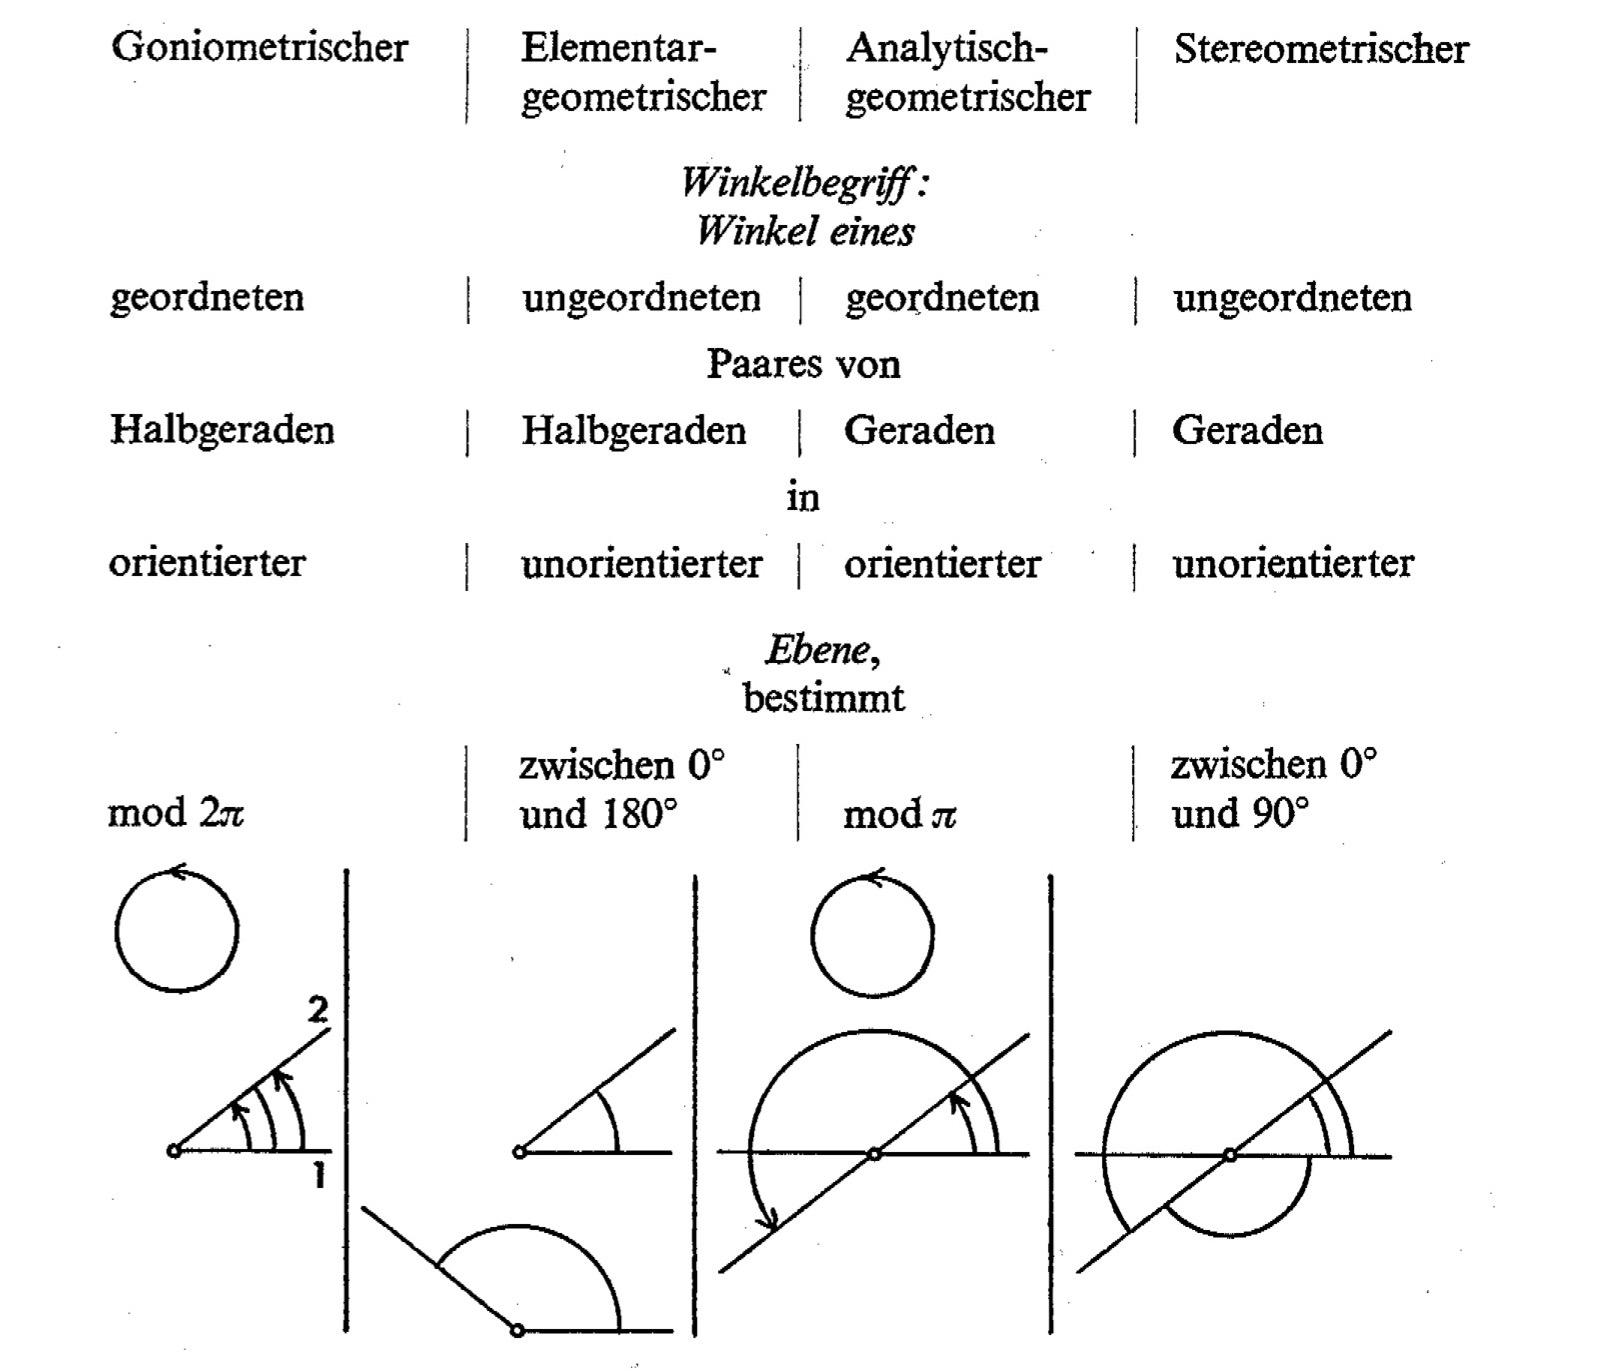
\includegraphics[width=0.75\linewidth]{pictures/1-FreudenthalWinkel} 

}

\caption{Winkelbegriffe nach Freudenthal (\protect\hyperlink{ref-Freudenthal:1973}{1973, S. 441})}\label{fig:FreudenthalWinkel}
\end{figure}

Er diskutiert, welchen Einfluss die jeweilige Sichtweise auf dem Maßbereich hat, wie Winkel überhaupt gemessen werden können und wie mit Winkeln operiert werden kann. Was passiert denn, wenn man ein geordnetes Strahlenpaar in der orientierten Ebene spiegelt (vgl. \protect\hyperlink{ref-Freudenthal:1973}{Freudenthal, 1973, S. 443~ff.})?

Wenn die Reihenfolge der Strahlen erhalten bleibt und die Winkelmessung aufgrund der Orientierung der Ebene vorgegeben ist, ändert sich damit ggf. auch das Maß des Winkels (siehe Abbildung \ref{fig:FreudenthalWinkelSpiegeln}).



\begin{figure}

{\centering 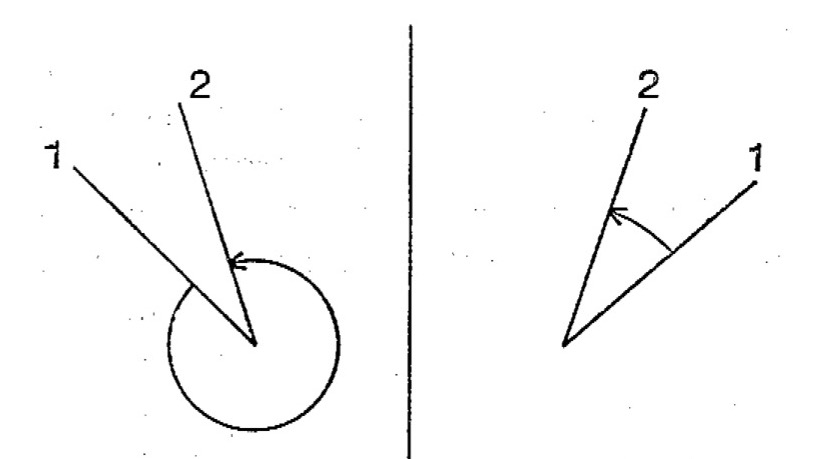
\includegraphics[width=0.5\linewidth]{pictures/1-FreudenthalWinkelSpiegeln} 

}

\caption{Spiegelung eines goniometrischen Winkels (\protect\hyperlink{ref-Freudenthal:1973}{Freudenthal, 1973, S. 443})}\label{fig:FreudenthalWinkelSpiegeln}
\end{figure}

Hierzu stellt Freudenthal (\protect\hyperlink{ref-Freudenthal:1973}{1973, S. 443~ff.}) weitere fachmathematische Ausführungen dar und schließt damit, dass der elementargeometrische, goniometrische und analytische Winkelbegriff aus fachlicher Sicht für den schulischen Lernpfad unentbehrlich sind (\protect\hyperlink{ref-Freudenthal:1973}{Freudenthal, 1973, S. 449}).

Die \emph{Spezifizierung} besteht also darin, den Begriff zu schärfen und Operationen mit ihm zu beschreiben. Die \emph{Strukturierung} besteht u.~a. in der vernetzenden Analyse der verschiedenen Winkelbegriffe und der Schlussfolgerung ihrer gleichermaßen Bedeutsamkeit für den Schulunterricht.\index{Vier-Ebenen-Ansatz!formale Ebene|)}

\hypertarget{semantische-ebene}{%
\subsection{Semantische Ebene}\label{semantische-ebene}}

Dazu,\index{Vier-Ebenen-Ansatz!semantische Ebene|(} welche Vorstellungen Schülerinnen und Schüler zum Winkelbegriff entwickeln sollen, sei u.~a. auf Krainer (\protect\hyperlink{ref-Krainer:1989}{1989}) und Mitchelmore \& White (\protect\hyperlink{ref-Mitchelmore:1998}{1998}) verwiesen. Eine grundsätzliche Schwierigkeit beim Unterrichten von Winkeln sind diverse und (scheinbar) nicht in Verbindung zu bringende Anwendungskontexte, die dennoch über denselben mathematischen Begriff beschrieben werden können. So ist das Sichtfeld eines Tieres ebenso wie die Umdrehung eines Wasserzählers über Winkel beschreibbar -- haben doch beide Situationen zunächst nichts miteinander zu tun.

Aufbauend auf den Arbeiten von Krainer (\protect\hyperlink{ref-Krainer:1989}{1989}) und Mitchelmore \& White (\protect\hyperlink{ref-Mitchelmore:1998}{1998}) können über eine Verknüpfung zur formalen Ebene mithilfe einer \emph{informationstheoretischen Winkeldefinition} (\protect\hyperlink{ref-Etzold2021}{Etzold, 2021, S. 39~f..}) vier Grundvorstellungen zum Winkelbegriff ausgearbeitet bzw. validiert werden:

\begin{itemize}
\tightlist
\item
  Winkel als Knick
\item
  Winkel als Feld
\item
  Winkel als Richtungsänderung
\item
  Winkel als Umdrehung
\end{itemize}

Dabei erhalten die \emph{Bestandteile} eines Winkels (Scheitelpunkt, Schenkel, ggf. Bereich zwischen den Schenkeln, Abweichungsmaß) eine besondere Bedeutung, über die sich auch eine sinnvolle Reihenfolge der Behandlung dieser Grundvorstellungen ableiten lässt. So »bietet es sich an, mit den Winkelfeldern zu beginnen. Bei diesen werden die meisten Bestandteile sichtbar (Scheitelpunkt, beide Schenkel als Begrenzungen sowie der zwischen den Schenkeln relevante Bereich) {[}\ldots{]}. Anschließend können Knicke oder Richtungsänderungen behandelt werden, woraufhin die Umdrehungen folgen.« (\protect\hyperlink{ref-Etzold2021}{Etzold, 2021, S. 60})

Die \emph{Spezifizierung} in diesem semantischen Teil ist demnach die Ausarbeitung der Grundvorstellungen. Die Begründung einer möglichen Reihenfolge kann der \emph{Strukturierung} des Lerngegenstands zugeordnet werden.\index{Vier-Ebenen-Ansatz!semantische Ebene|)}

\hypertarget{konkrete-ebene}{%
\subsection{Konkrete Ebene}\label{konkrete-ebene}}

Um\index{Vier-Ebenen-Ansatz!konkrete Ebene|(} die einzelnen Vorstellungen zu Winkeln aufzubauen, bedarf es charakteristischer Situationen, an denen der mathematische Kern der jeweiligen Vorstellung besonders gut sichtbar wird. Abbildung \ref{fig:Winkelsituationen} zeigt derartige \emph{Winkelsituationen} und die zugehörigen Grundvorstellungen (hier \emph{Winkelkontexte}).



\begin{figure}

{\centering 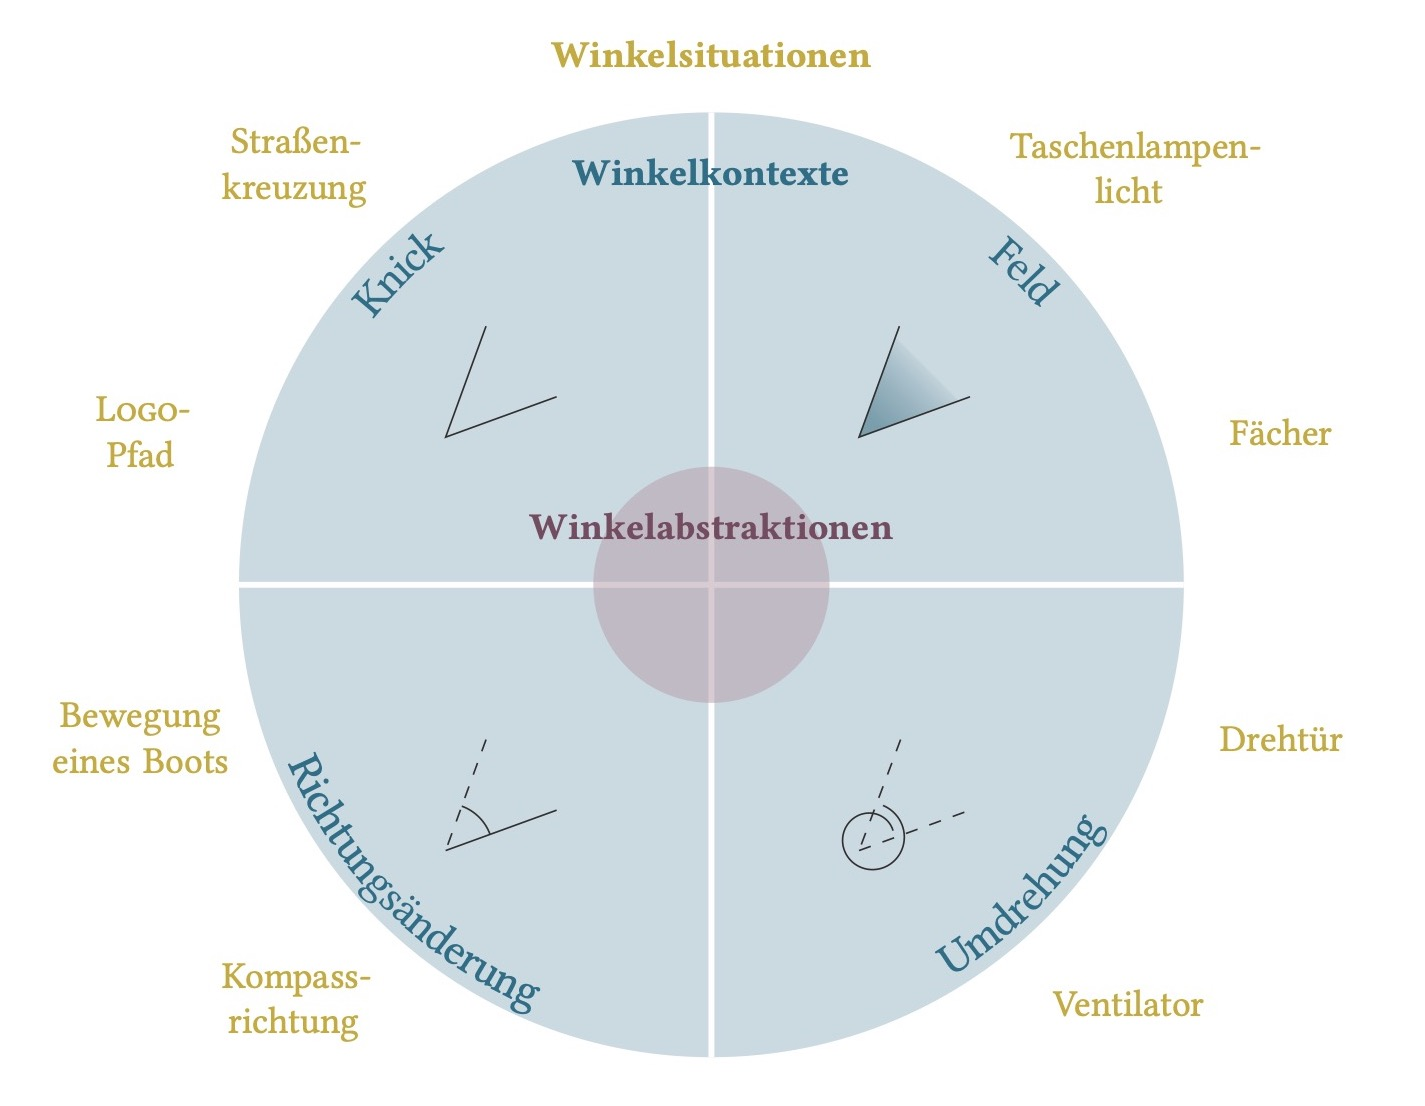
\includegraphics[width=0.75\linewidth]{pictures/1-Winkelsituationen} 

}

\caption{Winkelsituationen und -kontexte (\protect\hyperlink{ref-Etzold2021}{Etzold, 2021, S. 70})}\label{fig:Winkelsituationen}
\end{figure}

Exemplarisch für die Grundvorstellung des Winkels als Feld wird darauf aufbauend eine Lernumgebung und darin eingebettetes Unterrichtsmaterial entwickelt, mithilfe dessen die Grundvorstellung ausgebildet werden kann. An der konkreten Situation der \emph{Sichtfelder von Tieren} sollen die Schülerinnen und Schüler Handlungen ausführen, die es ihnen ermöglicht, den mathematischen Kern hinter dem konkreten Beispiel zu erkunden.

Die Schülerinnen und Schüler nutzen dazu eine App (siehe Abbildung \ref{fig:WinkelfarmApp}), in der mehrere Tiere mit ihren Sichtfeldern dargestellt werden können, und erhalten u.~a. folgende Aufgaben (vgl. \protect\hyperlink{ref-Etzold:2019Praxis4}{Etzold, 2019b, S. 8~ff.}):

\begin{enumerate}
\def\labelenumi{\arabic{enumi}.}
\tightlist
\item
  Setze das Schaf an eine Stelle, an der es von der Kuh gesehen wird, aber die Kuh selbst nicht sieht.
\item
  Setze das Schaf an eine Stelle, an der es nicht von der Kuh gesehen wird.
\item
  Das Schaf will die Kuh verwirren. Bewege es an möglichst viele Orte, an denen es von der Kuh gesehen wird.
\item
  Setze das Schaf an eine Stelle, an der es noch gerade so von der Kuh gesehen wird.
\item
  Wo muss das Schaf lang laufen, damit es die gesamte Zeit gerade so von der Kuh gesehen wird?
\end{enumerate}

An Aufgabe 5 kann z.~B. erkundet werde, dass sich das Schaf geradlinig auf der Grenze zwischen Sichtfeld und Nicht-Sichtfeld bewegen muss. In die eine Richtung ist die Bewegung beliebig fortsetzbar, in die andere durch den Kopf der Kuh begrenzt. Eine mathematische Verallgemeinerung dieser Handlung besteht dann in der Identifizierung des Schenkels (Begrenzung) als Strahl (nur in eine Richtung fortsetzbar) mit dem Scheitelpunkt (Kopf der Kuh) als \emph{Quelle} des Winkelfeldes.



\begin{figure}

{\centering 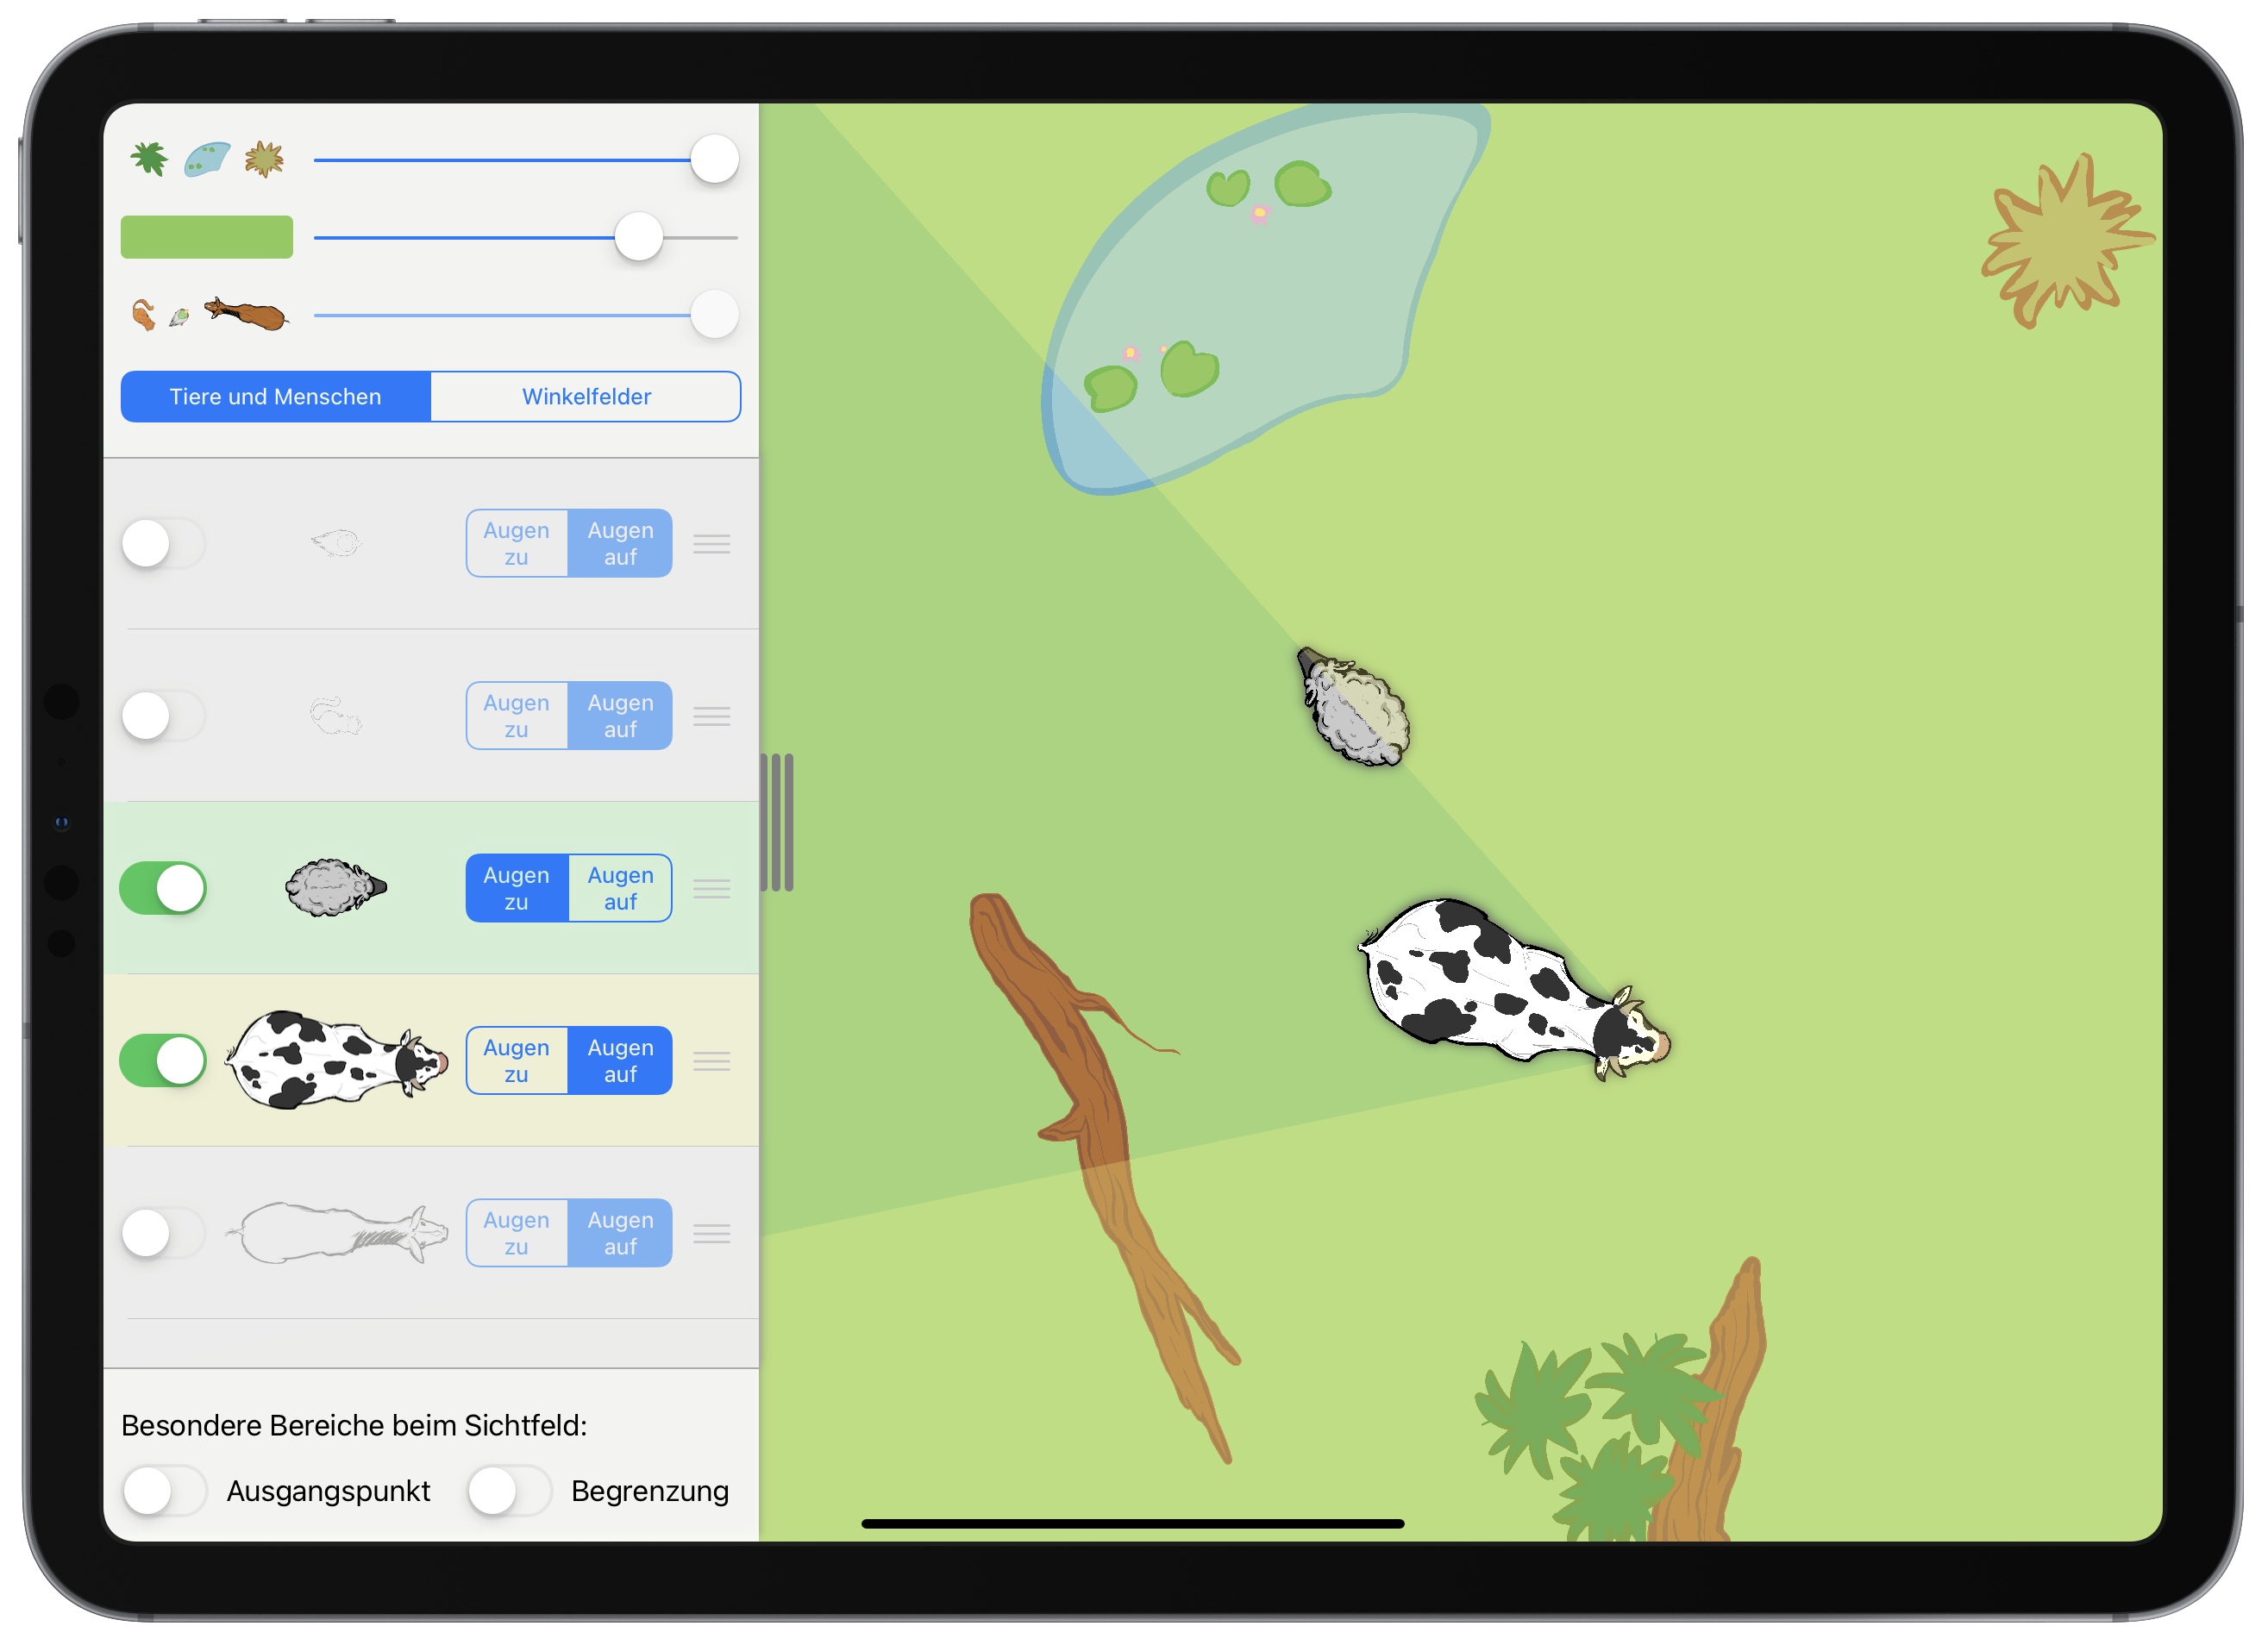
\includegraphics[width=0.75\linewidth]{pictures/1-Winkelfarm} 

}

\caption{Screenshot der App Winkel-Farm (\protect\hyperlink{ref-Etzold:2019}{Etzold, 2019a})}\label{fig:WinkelfarmApp}
\end{figure}

Als \emph{Spezifizierung} kann das Finden der Sichtfeld-Situation als charakterisches Beispiel für ein Winkelfeld angesehen werden. Die \emph{Strukturierung} führt zum dargestellten Lernpfad und den konkreten Aufgabenstellung, über die konkrete Handlungen verallgemeinert werden und damit das mathematische Verständnis aufgebaut wird.\index{Vier-Ebenen-Ansatz!konkrete Ebene|(}

\hypertarget{empirische-ebene}{%
\subsection{Empirische Ebene}\label{empirische-ebene}}

Die\index{Vier-Ebenen-Ansatz!empirische Ebene|(} zuvor beschriebene Lernumgebung wurde in mehreren Zyklen erprobt und dabei die Qualität der Handlungen der Schülerinnen und Schüler beobachtet. Ein Ziel bestand darin, dass möglichst verallgemeinerbare Handlungen (wie oben am Beispiel des Schenkels beschrieben) durchgeführt werden.

Es wird erwartet, dass die Repräsentation eines Sichtfeldes von der Draufsicht über eine semintransparent ausgemalte Teilfläche der Ebene noch nicht bekannt ist. Um diese nachzuvollziehen und mit eigenen Erfahrungen in Bezug zu bringen, wird an den Beginn der Unterrichtsstunde ein Bild des Klassenraumes in der Draufsicht präsentiert (siehe Abbildung \ref{fig:Klassenraum}). Dann soll eine Schülerin oder ein Schüler beschreiben, was sie/er alles sieht, ohne den Kopf zu drehen. Dieser Bereich wird auf dem Bild eingezeichnet, so dass die Repräsentation des Sichtfeldes im Folgenden zur Verfügung steht.

\begin{figure}

{\centering 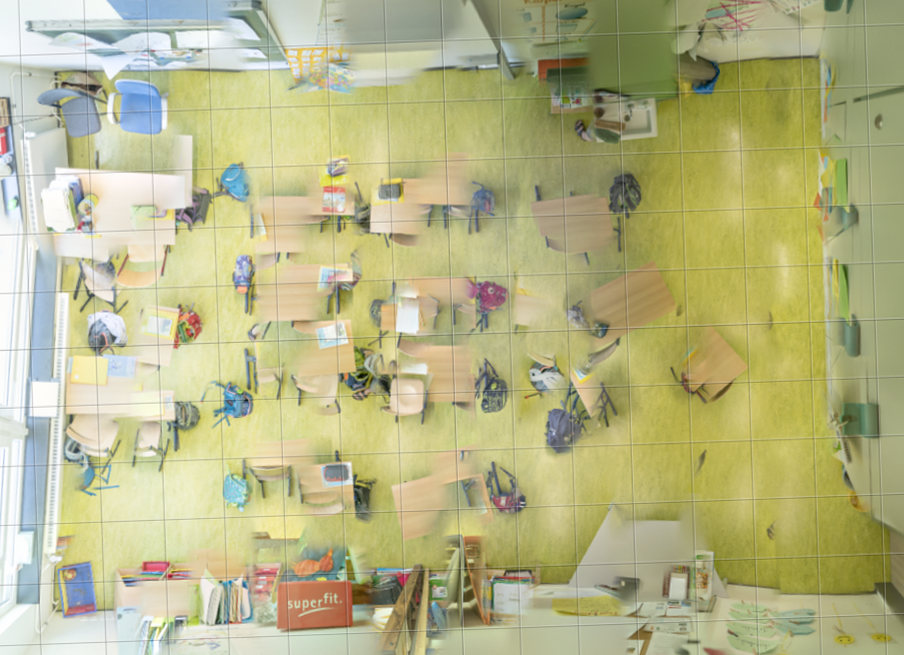
\includegraphics[width=0.75\linewidth]{pictures/1-Klassenraum} 

}

\caption{Klassenraum von oben (Foto: Christian Dohrmann)}\label{fig:Klassenraum}
\end{figure}

In der Erprobung konnte beobachtet werden, dass einige Bedienschwierigkeiten mit der Anwendung den Lernfortschritt hemmten. Dies konnte u.~a. dadurch verbessert werden, dass vor die eigentliche Erarbeitung eine freie Erkundungsphase mit der App (siehe Abbildung \ref{fig:WinkelfarmStart}) gesetzt wurde (\protect\hyperlink{ref-Etzold2021}{Etzold, 2021, S. 147, 152}). Durch spezifische Aufgabenstellungen wurden bestimmte Funktionen der App fokussiert:

\begin{figure}

{\centering 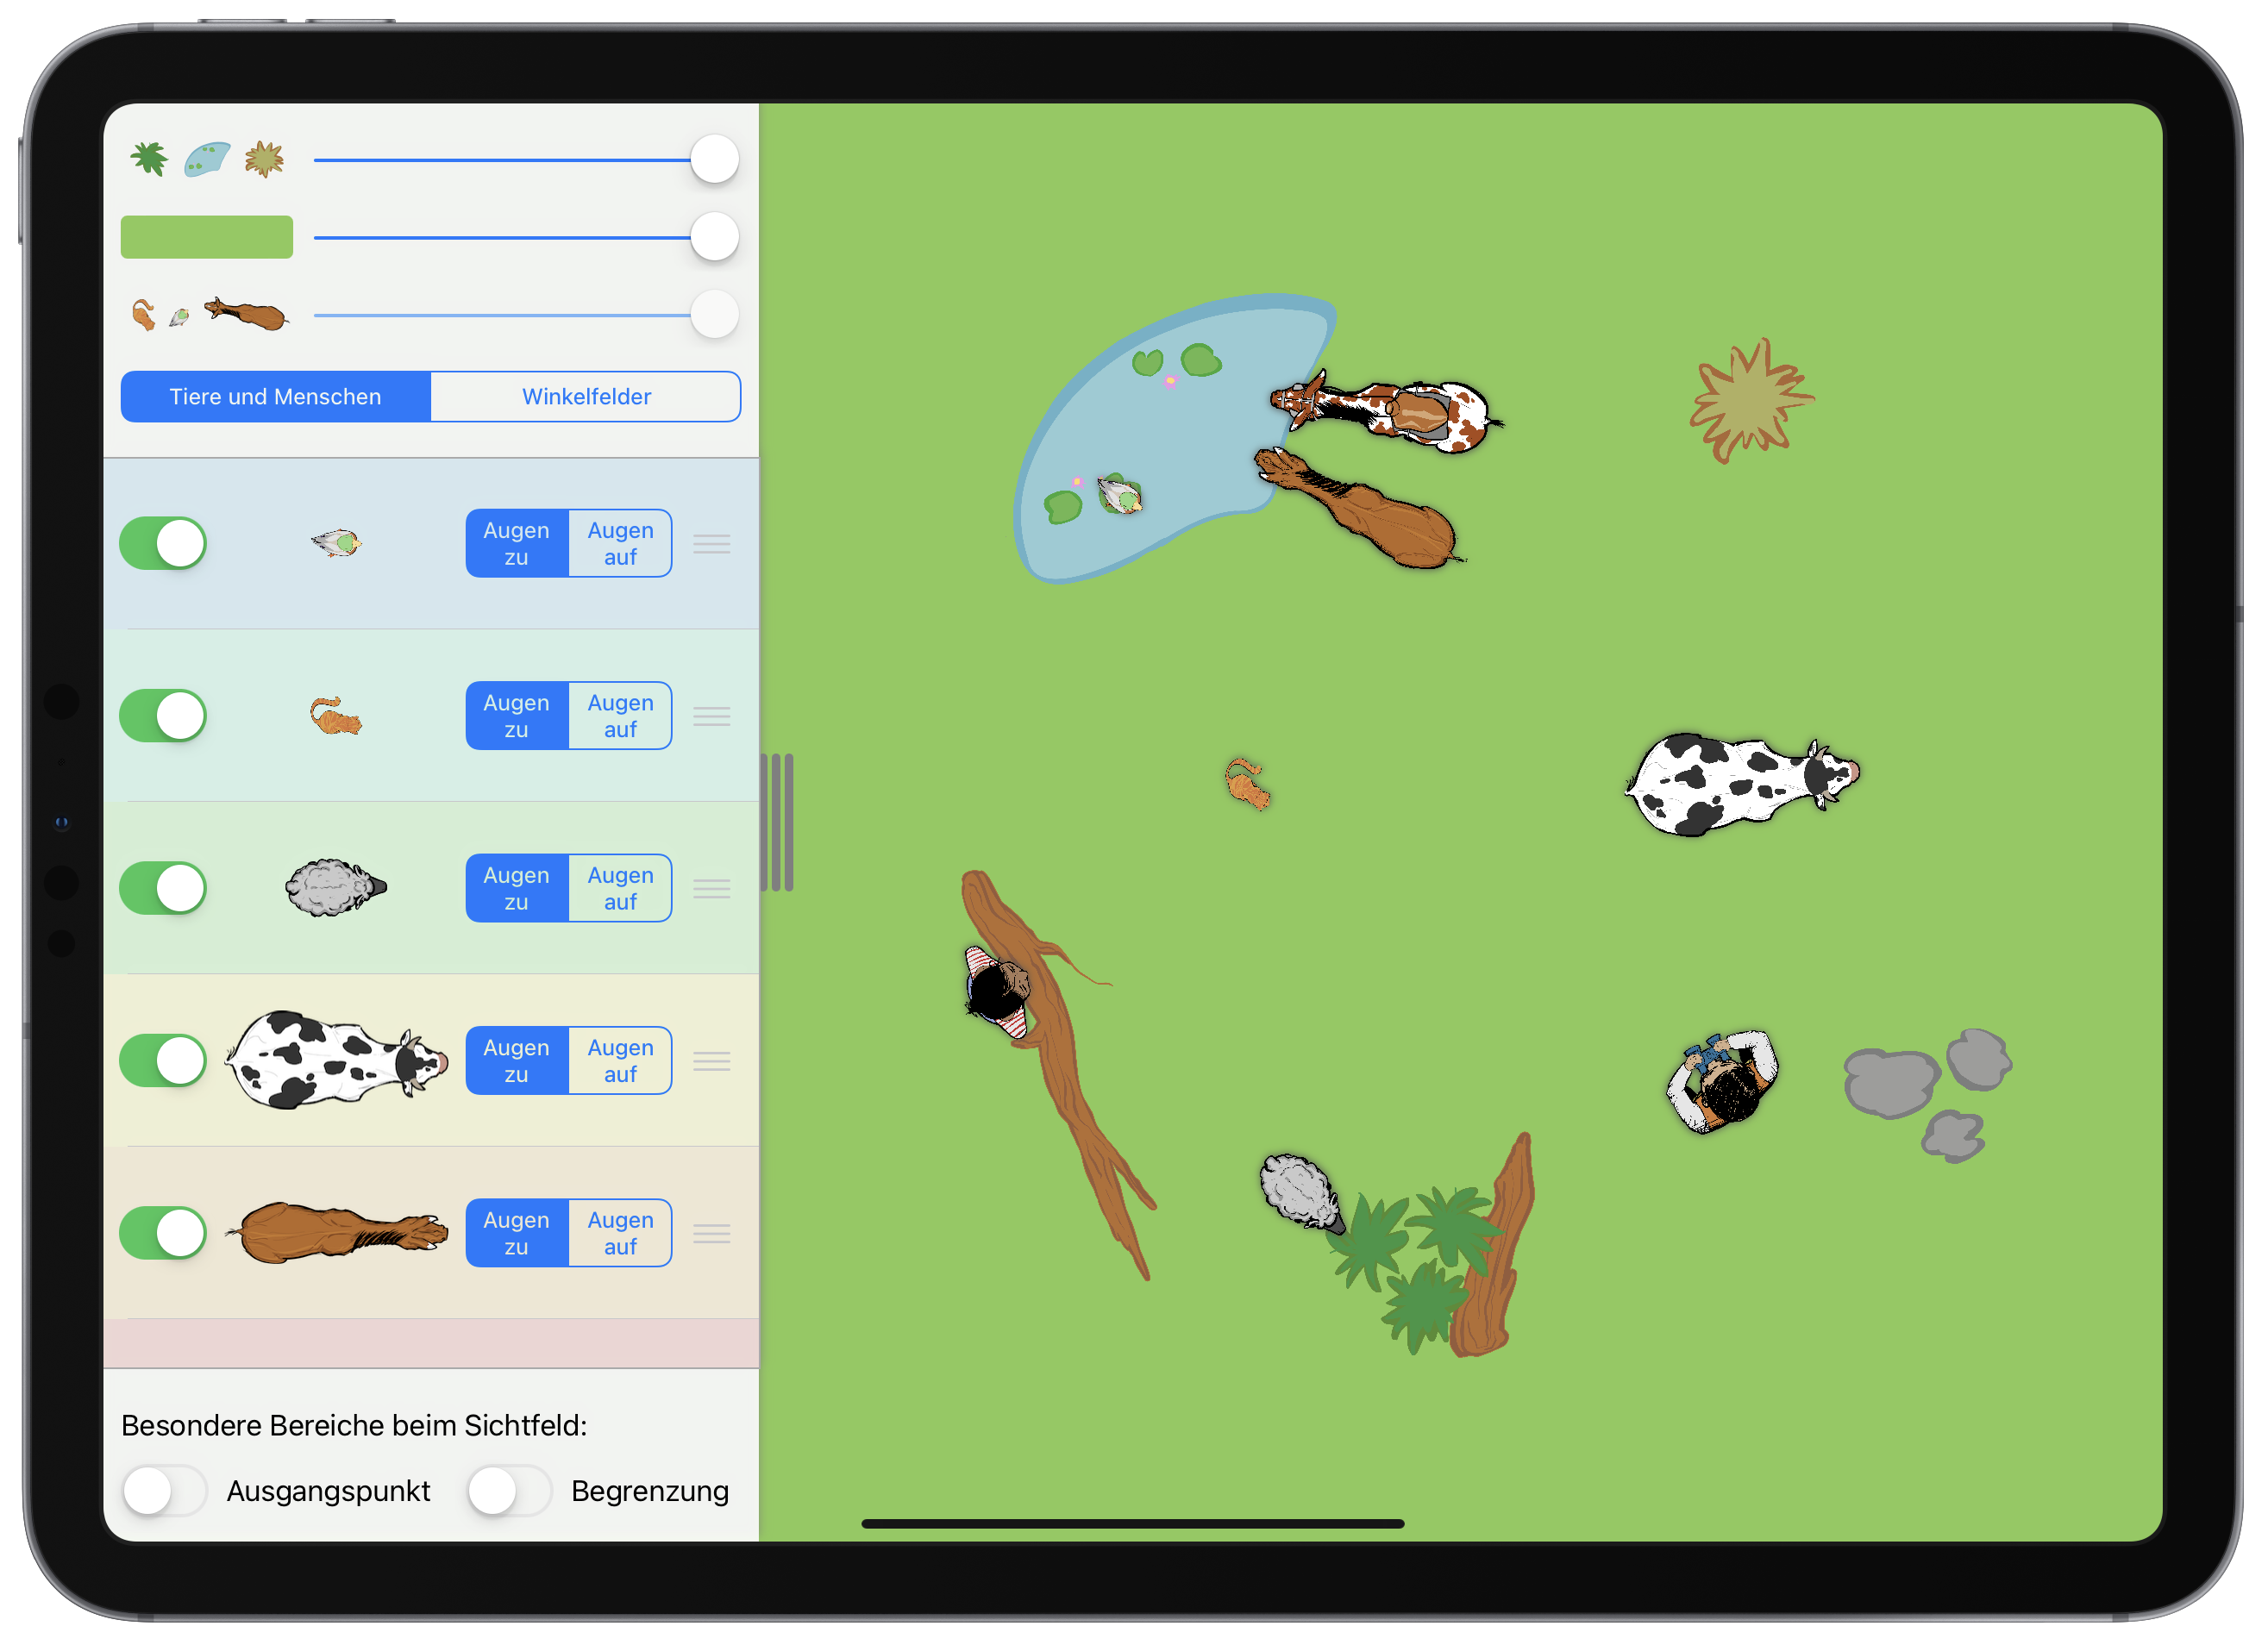
\includegraphics[width=0.75\linewidth]{pictures/1-WinkelfarmStart} 

}

\caption{Möglicher Startbildschirm für die freie Erkundungphase}\label{fig:WinkelfarmStart}
\end{figure}

\emph{»Das Pferd soll auf dem Steinpflaster stehen, die Frau soll auf dem Pferd sitzen/stehen. Das Pferd guckt in Richtung der grünen Büsche, die Frau hat die Augen zu. Gleichzeitig versteckt sich die Katze unter der Kuh.«}

Die Einführungsphase über das Klassenraumfoto folgt aus der \emph{Spezifizierung} innerhalb der empirischen Ebene. Das Hinzufügen der freien Erkundungsphase ist dagegen der \emph{Strukturierung} der Analyse zuzuordnen.\index{Winkel|)}\index{Vier-Ebenen-Ansatz!empirische Ebene|)}

\hypertarget{verknuxfcpfung-der-ebenen}{%
\subsection{Verknüpfung der Ebenen}\label{verknuxfcpfung-der-ebenen}}

An den Ausführungen ist schon sichtbar geworden, dass sich die Ebenen nicht immer trennen lassen und teilweise gegenseitig beeinflussen. Auch gehen oft Spezifizierung und Strukturierung ineinander über.

Das ist aber gar nicht schlimm, ganz im Gegenteil. Es zeigt wieder einmal, wie wichtig solch ein ganzheitlicher Ansatz ist, so dass eine stoffdidaktische Analyse aus den diversen Sichtpunkten heraus betrachtet werden sollte.

Wichtig ist v.~a., dass Sie sich als Lehrkraft stets darüber im Klaren sind, dass für eine stoffdidaktische Analyse verschiedene Perspektiven verfolgt werden müssen. Sehen Sie den Vier-Ebenen-Ansatz daher auch als Kontrollinstrument, ob Sie an alles gedacht haben, wenn Sie einen Lerngegenstand intensiv analysieren.

\hypertarget{vier-ebenen-nachbereitung}{%
\section{Zum Nachbereiten}\label{vier-ebenen-nachbereitung}}

\begin{enumerate}
\def\labelenumi{\arabic{enumi}.}
\tightlist
\item
  Lesen Sie den Artikel von Hußmann \& Prediger (\protect\hyperlink{ref-Hussmann:2016}{2016}) zum Vier-Ebenen-Ansatz.
\item
  Reflektieren Sie Ihre bisherige Fach- und Fachdidaktikausbildung in Mathematik dahingehend, welche der aufgeworfenen Fragen Sie zu konkreten Themenbereichen (nicht) beantworten könnten.
\end{enumerate}

\hypertarget{fundamentale-ideen}{%
\chapter{Fundamentale Ideen}\label{fundamentale-ideen}}

\begin{quote}
\textbf{Ziele}

\begin{itemize}
\tightlist
\item
  Sie können Fundamentale Ideen über ihre Kriterien definieren.
\item
  Sie kennen Beispiele für Fundamentale Ideen, auch über die in den Bildungsstandards beschriebenen Kompetenzen hinaus.
\item
  Sie können bei einzelnen Unterrichtsinhalten den Zusammenhang zu zugehörigen Fundamentalen Ideen herstellen.
\end{itemize}

\textbf{Material}

\begin{itemize}
\tightlist
\item
  Folien zur Vorlesung zu Fundamentalen Ideen (\href{files/Stoffdidaktik-WiSe2223-Kap2.pdf}{pdf}, \href{files/Stoffdidaktik-WiSe2223-Kap2.key}{Keynote})
\end{itemize}
\end{quote}

\hypertarget{fundamentale-ideen-begriffsklaerung}{%
\section{Begriffsklärung}\label{fundamentale-ideen-begriffsklaerung}}

Die Entwicklung Fundamentaler Ideen beruft sich auf Bruners Annahme, dass »jedes Kind {[}\ldots{]} auf jeder Entwicklungsstufe jeder Lehrgegenstand in einer intellektuell ehrlichen Form erfolgreich gelehrt werden« kann (vgl. \protect\hyperlink{ref-Bruner:1976}{Bruner, 1976, S. 77}). Voraussetzung dafür ist, dass die \emph{Struktur} eines Inhaltsbereichs in einer Art und Weise präsentiert wird, dass sie dem Kind zugänglich wird. Diese \emph{hinter den Dingen} liegende Struktur hebt sich vom konkreten Inhaltsbereich ab, ist allgemeinerer Natur und kann daher über \emph{Fundamentale Ideen} beschrieben werden.

Ziel der Orientierung des Unterrichtens an Fundamentalen Ideen besteht v.~a. darin, die (oftmals) isolierten Stoffelemente einzuordnen und in einem größeren Ganzen zu sehen. Im Umkehrschluss heißt dies aber auch, dass die Auswahl des konkreten Stoffes daran orientiert sein muss, wie dieser dazu beitragen kann, den dahinter liegenden mathematischen Kern und die zugehörigen Fundamentalen Ideen zu vertreten.

Die dazu seit den 1960er Jahren in Gang gesetzte Forschung führte zu vielfältigen Vorschlägen Fundamentaler Ideen der Mathematik -- jedoch bisher nicht zu einem allgemeingültigen Katalog. Dieser Vielfalt in den Formulierungen und Kategorisierungen kann begegnet werden, indem Fundamentale Ideen über Eigenschaften charakterisiert werden. Im Rahmen dieser Veranstaltung wird folgende Definition genutzt, zitiert aus Schwill (\protect\hyperlink{ref-Schwill:1994}{1994}).

\begin{definition}[Fundamentale Idee]
\protect\hypertarget{def:FundamentaleIdee}{}\label{def:FundamentaleIdee}

Eine \textbf{Fundamentale Idee}\index{Fundamentale Idee|textbf} bzgl. eines Gegenstandsbereichs (Wissenschaft, Teilgebiet) ist ein \textbf{Denk-, Handlungs-, Beschreibungs- oder Erklärungsschema}, das

\begin{enumerate}
\def\labelenumi{\arabic{enumi}.}
\tightlist
\item
  in verschiedenen Gebieten des Bereichs vielfältig anwendbar oder erkennbar ist (\textbf{Horizontalkriterium}),\index{Fundamentale Idee!Horizontalkriterium|textbf}
\item
  auf jedem intellektuellen Niveau aufgezeigt und vermittelt werden kann (\textbf{Vertikalkriterium}),\index{Fundamentale Idee!Vertikalkriterium|textbf}
\item
  in der historischen Entwicklung des Bereichs deutlich wahrnehmbar ist und längerfristig relevant bleibt (\textbf{Zeitkriterium}),\index{Fundamentale Idee!Zeitkriterium|textbf}
\item
  einen Bezug zu Sprache und Denken des Alltags und der Lebenswelt besitzt (\textbf{Sinnkriterium}).\index{Fundamentale Idee!Sinnkriterium|textbf}
\end{enumerate}

\end{definition}

\begin{quote}
\textbf{Überblick zur historischen Entwicklung Fundamentaler Ideen}

\begin{itemize}
\tightlist
\item
  von der Bank (\protect\hyperlink{ref-Bank:2016}{2016, S. 37~ff.}): \emph{Fundamentale Ideen der Mathematik: Weiterentwicklung einer Theorie zu deren unterrichtspraktischer Nutzung}
\end{itemize}
\end{quote}

\hypertarget{auswahl-fundamentaler-ideen}{%
\section{Auswahl fundamentaler Ideen}\label{auswahl-fundamentaler-ideen}}

\hypertarget{kategorisierung}{%
\subsection{Kategorisierung}\label{kategorisierung}}

Das Fehlen eines allgemeingültigen Katalogs sollte nicht davon abhalten, bestehende Auflistungen und Strukturierungen Fundamentaler Ideen zu betrachten. Angelehnt an von der Bank (\protect\hyperlink{ref-vonderBank:2013}{2013, S. 103}) und Lambert (\protect\hyperlink{ref-Lambert:2012}{2012}), die unterschiedliche Kategorisierungen analysiert haben, sollen an dieser Stelle drei grobe Bereiche festgehalten werden.

\hypertarget{inhaltsideen}{%
\subsubsection{Inhaltsideen}\label{inhaltsideen}}

Inhaltsideen beziehen sich auf konkrete Inhaltsbereiche der Mathematik, die die Kriterien Fundamentaler Ideen erfüllen können. Nicht ganz zufällig spiegeln diese sich in den Leitideen der Bildungsstandards wider (\protect\hyperlink{ref-KMK:2012}{Sekretariat der Ständigen Konferenz der Kultusminister der Länder in der Bundesrepublik Deutschland, 2012}, \protect\hyperlink{ref-SekretariatderStandigenKonferenzderKultusministerderLanderinderBundesrepublikDeutschland2022}{2022a}, \protect\hyperlink{ref-SekretariatderStandigenKonferenzderKultusministerderLanderinderBundesrepublikDeutschland2022a}{2022b}).

Beispiele:

\begin{itemize}
\tightlist
\item
  Zahl
\item
  Algorithmus
\item
  Maß
\item
  Raum und Form
\item
  Funktion
\item
  Zufall
\end{itemize}

\hypertarget{schnittstellenideen}{%
\subsubsection{Schnittstellenideen}\label{schnittstellenideen}}

Schnittstellenideen haben die Eigenschaft, dass durch sie die »Mathe(matik) wirkt« und »auch für andere Fächer in ihrer je spezifischen Weise relevant sind« (\protect\hyperlink{ref-Lambert:2012}{Lambert, 2012}). Damit korrelieren sie mit den prozessbezogenen Kompetenzen der Bildungsstandards.

Beispiele:

\begin{itemize}
\tightlist
\item
  Kommunizieren
\item
  Modellieren
\item
  Argumentieren
\item
  Problemlösen
\item
  Darstellen
\item
  Fragen
\end{itemize}

\hypertarget{taetigkeitsideen}{%
\subsubsection{Tätigkeitsideen}\label{taetigkeitsideen}}

Tätigkeitsideen beziehen sich insbesondere auf innermathematische Tätigkeiten, die sich über verschiedene Inhaltsbereiche hinweg zeigen. Lambert (\protect\hyperlink{ref-Lambert:2012}{2012}) betont, dass es diese (über die Bildungsstandards hinaus) ebenfalls zu beachten gilt, wenn man einen reichhaltigen Mathematikunterricht bewirken möchte.

Beispiele:

\begin{itemize}
\tightlist
\item
  Approximierung
\item
  Optimierung
\item
  Linearität/Linearisierung
\item
  Symmetrie
\item
  Invarianz
\item
  Rekursion
\item
  Vernetzung
\item
  Ordnen
\item
  Strukturierung
\item
  Formalisierung
\item
  Exaktifizierung
\item
  Verallgemeinern
\item
  Idealisieren
\end{itemize}

Im Rahmen des Projektmoduls \emph{Erweitertes Fachwissen für den schulischen Kontext in Mathematik}\footnote{siehe Modulbeschreibung bei \href{https://puls.uni-potsdam.de/qisserver/rds?state=verpublish\&status=init\&vmfile=no\&moduleCall=modulansicht\&publishConfFile=modulverwaltung\&publishSubDir=up/modulbearbeiter\&\&modul.modul_id=3156\&menuid=\&topitem=Modulbeschreibung\&subitem=}{PULS}} werden Sie insbesondere Bezüge zwischen Schul- und Hochschulmathematik auf Basis Fundamentaler Ideen herstellen, wofür die Inhalts- und Tätigkeitsideen von hoher Relevanz sind.

\begin{quote}
\textbf{Diskussion Fundamentaler Ideen in den Stoffgebieten der Sekundarstufe II}

\begin{itemize}
\tightlist
\item
  Analysis: Tietze et al. (\protect\hyperlink{ref-Tietze:2000a}{2000a})
\item
  Lineare Algebra/Analytische Geometrie: Tietze et al. (\protect\hyperlink{ref-Tietze:2000}{2000b})
\item
  Stochastik: Tietze et al. (\protect\hyperlink{ref-Tietze:2002}{2002})
\end{itemize}
\end{quote}

\hypertarget{beispiel-linearitaet}{%
\subsection{Beispiel Linearität}\label{beispiel-linearitaet}}

\hypertarget{horizontal--und-vertikalkriterium}{%
\subsubsection{Horizontal- und Vertikalkriterium}\label{horizontal--und-vertikalkriterium}}

Linearität\index{Linearität|(}\index{Fundamentale Idee!Horizontalkriterium|(}\index{Fundamentale Idee!Vertikalkriterium|(} ist ein wesentliches Konzept über die gesamte Schullaufbahn hinweg (und darüber hinaus). Dies spiegelt sich in vielfältigen Themenbereichen wider, die sowohl die Breite (\emph{Horizontalkriterium}) als auch Tiefe (\emph{Vertikalkriterium}) von Linearität und (später) auch Linearisierung zeigen. Dieser Abschnitt orientiert sich an den Darstellungen von Danckwerts (\protect\hyperlink{ref-Danckwerts:1988}{1988}).

\begin{itemize}
\tightlist
\item
  Linearität als Phänomen tritt schon im Geometrieunterricht der Grundschule mit \textbf{Geraden} als essentielle geometrische Objekte auf. In der euklidischen Geometrie sind Geraden neben Punkten die Basisobjekte eines axiomatischen Aufbaus.
\item
  Das \textbf{Distributivgesetz} \(a\cdot (b+c) = a\cdot b + a\cdot c\), das ebenfalls bereits in der Grundschule behandelt wird, beschreibt einen linearen Vorgang und bietet die Grundlage für die halbschriftliche Multiplikation. Über die Schulmathematik hinaus dient es z.~B. als eines der Vektorraumaxiome (Skalarmultiplikation).
\item
  Das Bestimmen eines \textbf{Rechteckflächeninhalts} ist ein linearer Vorgang: Ein Rechteck, das doppelt so breit ist, hat (bei gleicher Höhe) einen doppelt so großen Flächeninhalt. Betrachtet man diese Eigenschaft nicht als Phänomen, sondern als Forderung an eine Flächeninhaltsformel, so kann aus den Bedingungen \(A(a_1+a_2,b) = A(a_1,b) + A(a_2,b)\) und \(A(a,b_1+b_2) = A(a,b_1)+A(a,b_2)\) sowie der Stetigkeit in \(\mathbb{R}^+\) die Formel \(A(a,b) = a\cdot b\) abgeleitet werden.
\item
  Lineare Zuordnungen der Art \(f(x+y) = f(x)+f(y)\) werden zu Beginn der Sekundarstufe I als \textbf{proportionale Zuordnungen} behandelt. Dies wird fortgeführt bei \textbf{linearen Funktionen} der Art \(f(x) = mx+n\), in der Fachmathematik als affin-lineare Abbildungen bezeichnet.
\item
  \textbf{Lineare Gleichungen und Gleichungssysteme} sind ebenfalls bedeutsamer Bestandteil des Mathematikunterrichts. Überhaupt baut die gesamte \textbf{Lineare Algebra} auf lineare und affin-lineare Abbildungen auf.
\item
  Die \textbf{Strahlensätze} beschreiben ebenfalls ein lineares Verhalten: Geradenabschnitte in \(c\)-facher Entfernung sind \(c\) mal so lang.
\end{itemize}

\begin{figure}

{\centering 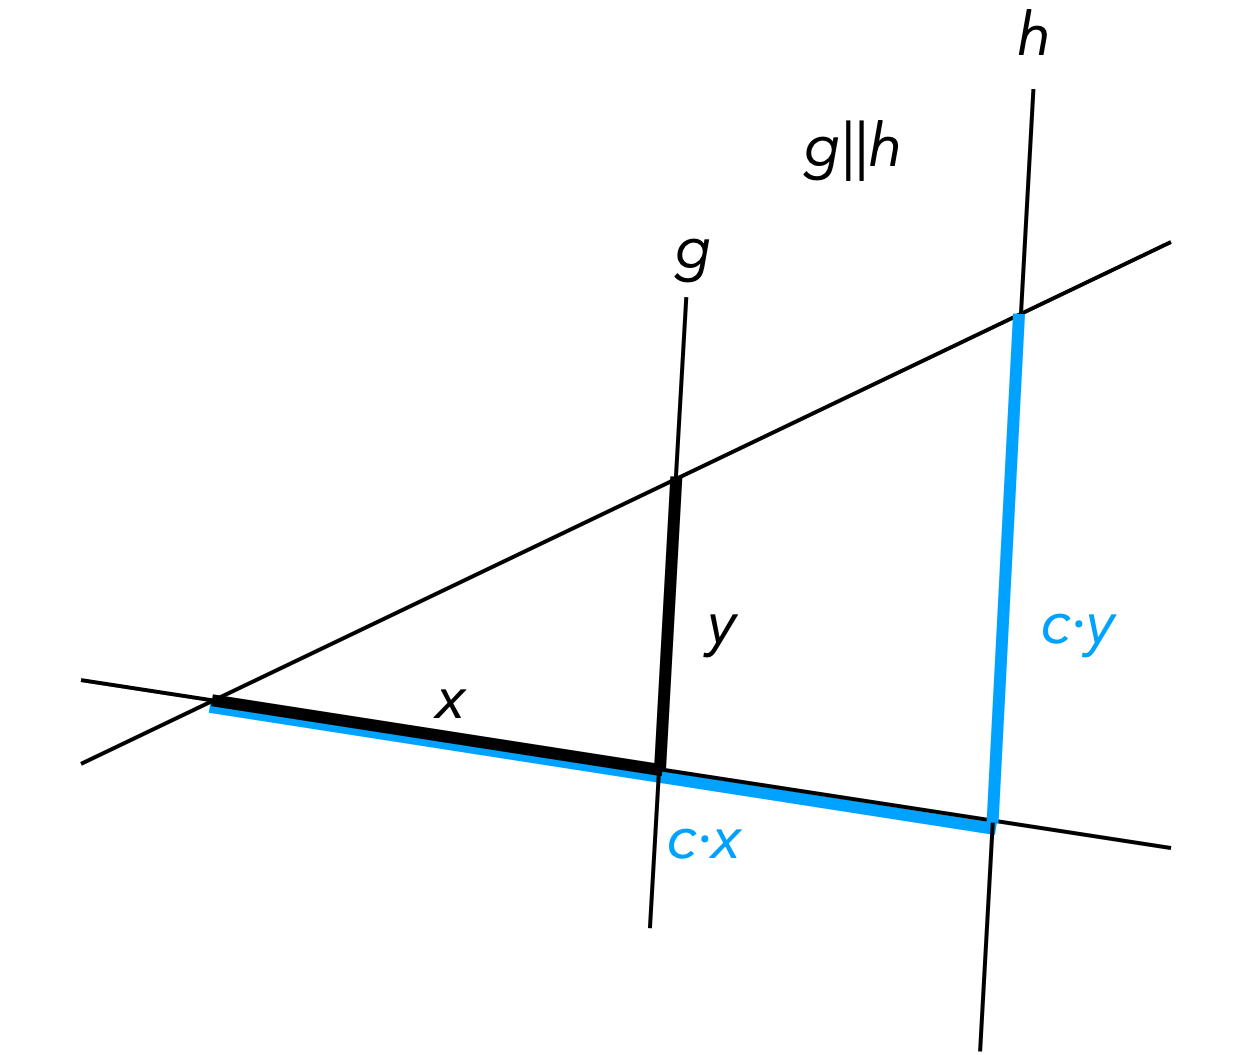
\includegraphics[width=0.5\linewidth]{pictures/2-Strahlensatz} 

}

\caption{Strahlensatzfigur}\label{fig:Strahlensatz}
\end{figure}

\begin{itemize}
\tightlist
\item
  Beim \textbf{Ableitungsbegriff} ist eine wesentliche Vorstellung, dass die Funktion in der Umgebung der zu betrachtenden Stelle linearisiert wird. Insbesondere bei höherdimensionalen Funktionen wird der Linearisierungsansatz weiterverfolgt. Die ebenfalls vorherrschende Tangentenvorstellung ist auf mehr als drei Dimensionen nicht mehr anschaulich übertragbar -- der Linearisierungsansatz weist hier aufgrund seiner algebraischen Beschreibung die bessere Verallgemeinerbarkeit auf.
\item
  Eng an den Linearisierungsansatz angelehnt ist die \textbf{lineare Approximation} von Funktionen (z.~B. \(\sin(x)\approx x\) für \(x\approx 0\)). Die führt sich in der Hochschulmathematik fort, beispielsweise bei Taylor-Reihen.
\item
  Das Bedürfnis der Linearisierung, insbesondere aus der Physik heraus, zeigt sich auch bei der Nutzung \textbf{spezifisch skalierter Diagrammachsen}, z.~B. von Logarithmuspapier. Wegen der Äquivalenz von \(y = c\cdot a^x\) und \(\ln y = (\ln a )\cdot x + \ln c\) lassen sich beliebige Exponentialfunktionen auf Logarithmuspapier als lineare Funktionen darstellen.
\item
  Verschiedene Näherungsverfahren, wie das \textbf{Newton-Verfahren}, bedienen sich ebenfalls der Linearisierung.
\end{itemize}

An dieser Stelle sei darauf hingewiesen, dass Linearität derart fundamental ist, dass selbst nicht-lineare Zusammenhänge häufig fälschlicherweise als linear angenommen werden. Dies zeigt sich zum Beispiel an den Fehlannahmen \((x+y)^2 \overset{?!}{=} x^2+y^2\), \(\sqrt{x+y} \overset{?!}{=} \sqrt{x}+\sqrt{y}\) oder \(\sin(x+y) \overset{?!}{=} \sin(x)+\sin(y)\). Derartige Fehler können Sie als Lehrkraft besser einordnen (und korrigieren), wenn Sie sich der Fundamentalen Idee \emph{Linearität} (die hier eben \emph{nicht} gilt) bewusst sind. Insbesondere spricht dies auch für ein Explizitmachen der Fundamentalen Idee Ihren Schülerinnen und Schülern gegenüber, so dass Sie derartigen Fehlern nicht nur mit Gegenbeispielen entgegen treten können, sondern auch eine strukturelle Einordnung sichtbar machen können.

Gerade wegen der genannten Fehlannahmen und der für die Schülerinnen und Schüler i.~d.~R. nicht in Zusammenhang gebrachten Dualität aus \emph{geradlinig} und \emph{additiv und homogen} sehen Tietze et al. (\protect\hyperlink{ref-Tietze:2002}{2002, S. 39}) die Linearität dagegen nicht als eine im Mathematikunterricht etablierte Fundamentale Idee, »die die Schüler erkennen und die ihr Denken ordnet und anregt«.\index{Fundamentale Idee!Horizontalkriterium|)}\index{Fundamentale Idee!Vertikalkriterium|)}

\hypertarget{zeit--und-sinnkriterium}{%
\subsubsection{Zeit- und Sinnkriterium}\label{zeit--und-sinnkriterium}}

Linearität\index{Fundamentale Idee!Zeitkriterium|(}\index{Fundamentale Idee!Sinnkriterium|(} zeigt sich auch in der historischen Entwicklung der Mathematik als eine prägende Leitlinie, womit sie das \emph{Zeitkriterium} Fundamentaler Ideen erfüllt. In der Linearen Algebra sei beispielsweise das Lösen linearer Gleichungssysteme im 18. Jahrhundert bis hin zum Gauß-Algorithmus im 19. Jahrhundert oder die Darstellung linearer Vorgänge mit Matrizen im 17./18. Jahrhundert erwähnt (vgl. \protect\hyperlink{ref-Tietze:2000}{Tietze et al., 2000b, S. 73~ff.}). In der Analysis spiegelt sich die Linearität bzw. Linearisierung in der gesamten Differenzialrechnung wider, von der Interpolation nach der Jahrtausendwende über Taylors \emph{Linear perspective} von 1715 (vgl. \protect\hyperlink{ref-Bruckler:2018}{Brückler, 2018, S. 39, 119}) bis in die Gegenwart der linearen Modellierung nichtlinearer Zusammenhänge.

\begin{quote}
\textbf{Historische Originalausgabe}

Taylor (\protect\hyperlink{ref-Taylor:1715}{1715}): \emph{Linear perspective}
\end{quote}

Auch Alltagssituationen bzw. die Alltagssprache ist von Linearität geprägt. Beispielsweise treten proportionale Zuordnungen unmittelbar beim Einkaufen auf, wenn Waren abgewogen und der Preis bestimmt wird. Auch reale Messvorgänge, wie z.~B. die Geschwindigkeitsmessung, beziehen sich in der Regel auf die Messung von (sehr kurzen) Zeitintervallen, in denen ein lineares Verhalten angenommen wird. Das \emph{Sinnkriterium} zeigt sich aber auch in Begriffen wie \emph{lineares Fernsehen} oder \emph{lineare Erzählungen}. Dies ist zwar keine mathematische Linearität im Sinne der Formel \(f(x+y) = f(x) +f(y)\), aber der Begriff findet in einer verwandten Bedeutung in der Alltagssprache Verwendung.\index{Linearität|)}\index{Fundamentale Idee!Zeitkriterium|)}\index{Fundamentale Idee!Sinnkriterium|)}

\hypertarget{gegenbeispiele}{%
\subsection{Gegenbeispiele}\label{gegenbeispiele}}

Zur Verständnisförderung sollen noch ein paar Gegenbeispiele für Fundamentale Ideen angebracht werden.

\begin{itemize}
\tightlist
\item
  Das bereits erwähnte \textbf{Distributivgesetz} an sich ist zwar elementar, aber ihm fehlt die Weite, womit es nicht das Horizontalkriterium erfüllt. Die \emph{Linearität} als dahinterliegende Idee ist dagegen weit genug (vgl. ähnliche Argumentation zum \textbf{Kommutativgesetz} und der dahinterliegenden Idee der \emph{Invarianz} bei \protect\hyperlink{ref-Schubert:2011}{Schubert \& Schwill, 2011, S. 63}).
\item
  Der \textbf{Umkehrfunktion} fehlt das Sinnkriterium, da dieser Begriff in der Lebenswelt außerhab der Mathematik kaum von Relevanz ist. Dahinter liegt vielmehr die Idee der \emph{Reversibilität} als »Umkehrbarkeit von Operationen mit Wiederherstellung des Ausgangszustandes« (\protect\hyperlink{ref-Schubert:2011}{Schubert \& Schwill, 2011, S. 63}).
\end{itemize}

\hypertarget{fund.-ideen-und-stoffdidaktik}{%
\section{Fund. Ideen und Stoffdidaktik}\label{fund.-ideen-und-stoffdidaktik}}

Fundamentale Ideen haben zwar ihren Ursprung in der Fachstruktur, aber sie »sind nicht Elemente der Wissenschaft an sich, sondern Produkte unseres Verstandes, die wir der Wissenschaft aufprägen. Folglich können sie nur relativ zum Menschen objektiviert werden« (\protect\hyperlink{ref-Schubert:2011}{Schubert \& Schwill, 2011, S. 62}). Hinsichtlich des \protect\hyperlink{tab:fragen-ebenen}{Vier-Ebenen-Ansatzes} liegen sie auf der \textcolor{semanticColor}{semantischen Ebene} mit starken Bezügen zur \textcolor{formalColor}{formalen Ebene}.

Für Ihre stoffdidaktische Analyse können Fundamentale Ideen insbesondere hilfreich für die \textbf{Dekonstruktion} des Fachwissens und anschließende \textbf{Rekonstruktion} des Schulwissens sein.

Wenn sie also beispielsweise eine stoffdidaktische Analyse zur Flächeninhaltsberechnung durchführen, setzen Sie sich mit der Fundamentalen Idee des \emph{Messens}\index{Messen} auseinander. Dabei verstehen Sie Messvorgänge als Vergleiche zu einem Standardmaß (z.~B. Kästchen auszählen), erkennen Zerlegungs- und Ergänzungsgleichheit als notwendige Prinzipien zur präziseren Beschreibung, sehen Dreiecke als bedeutsame Basisfiguren für Flächeninhaltsberechnungen an und haben den Blick für die Integralrechnung als verallgemeinerbare Methode zur Flächeninhaltsbestimmung krummliniger Figuren (vgl. \protect\hyperlink{ref-Vohns:2000}{Vohns, 2000, S. 98~ff.}). Sie \emph{dekonstruieren} (zerlegen) damit Ihr eigenes mathematisches Fachwissen.

Nun sind Sie in der Lage, das Wissen zur Flächeninhaltsberechnung für Schülerinnen und Schüler neu aufzubauen, also zu \emph{rekonstruieren} und (unter Hinzunahme der Betrachtung von Grundvorstellungen und den restlichen Ebenen des Vier-Ebenen-Ansatzes) einen Lernpfad zu entwickeln. Im Zusammenhang mit der Integralrechnung kann dies z.~B. heißen, dass Sie parallel zum Bilden von Ober- und Untersummen noch einmal eine krummlinig begrenzte Fläche durch Kästchen auszählen lassen -- ggf. mit unterschiedlicher Feinheit und einer Abschätzung nach oben und nach unten. Die Fundamentalen Ideen haben für Sie damit auch eine \emph{ordnende Funktion} des Unterrichtsstoffes.

\begin{figure}

{\centering 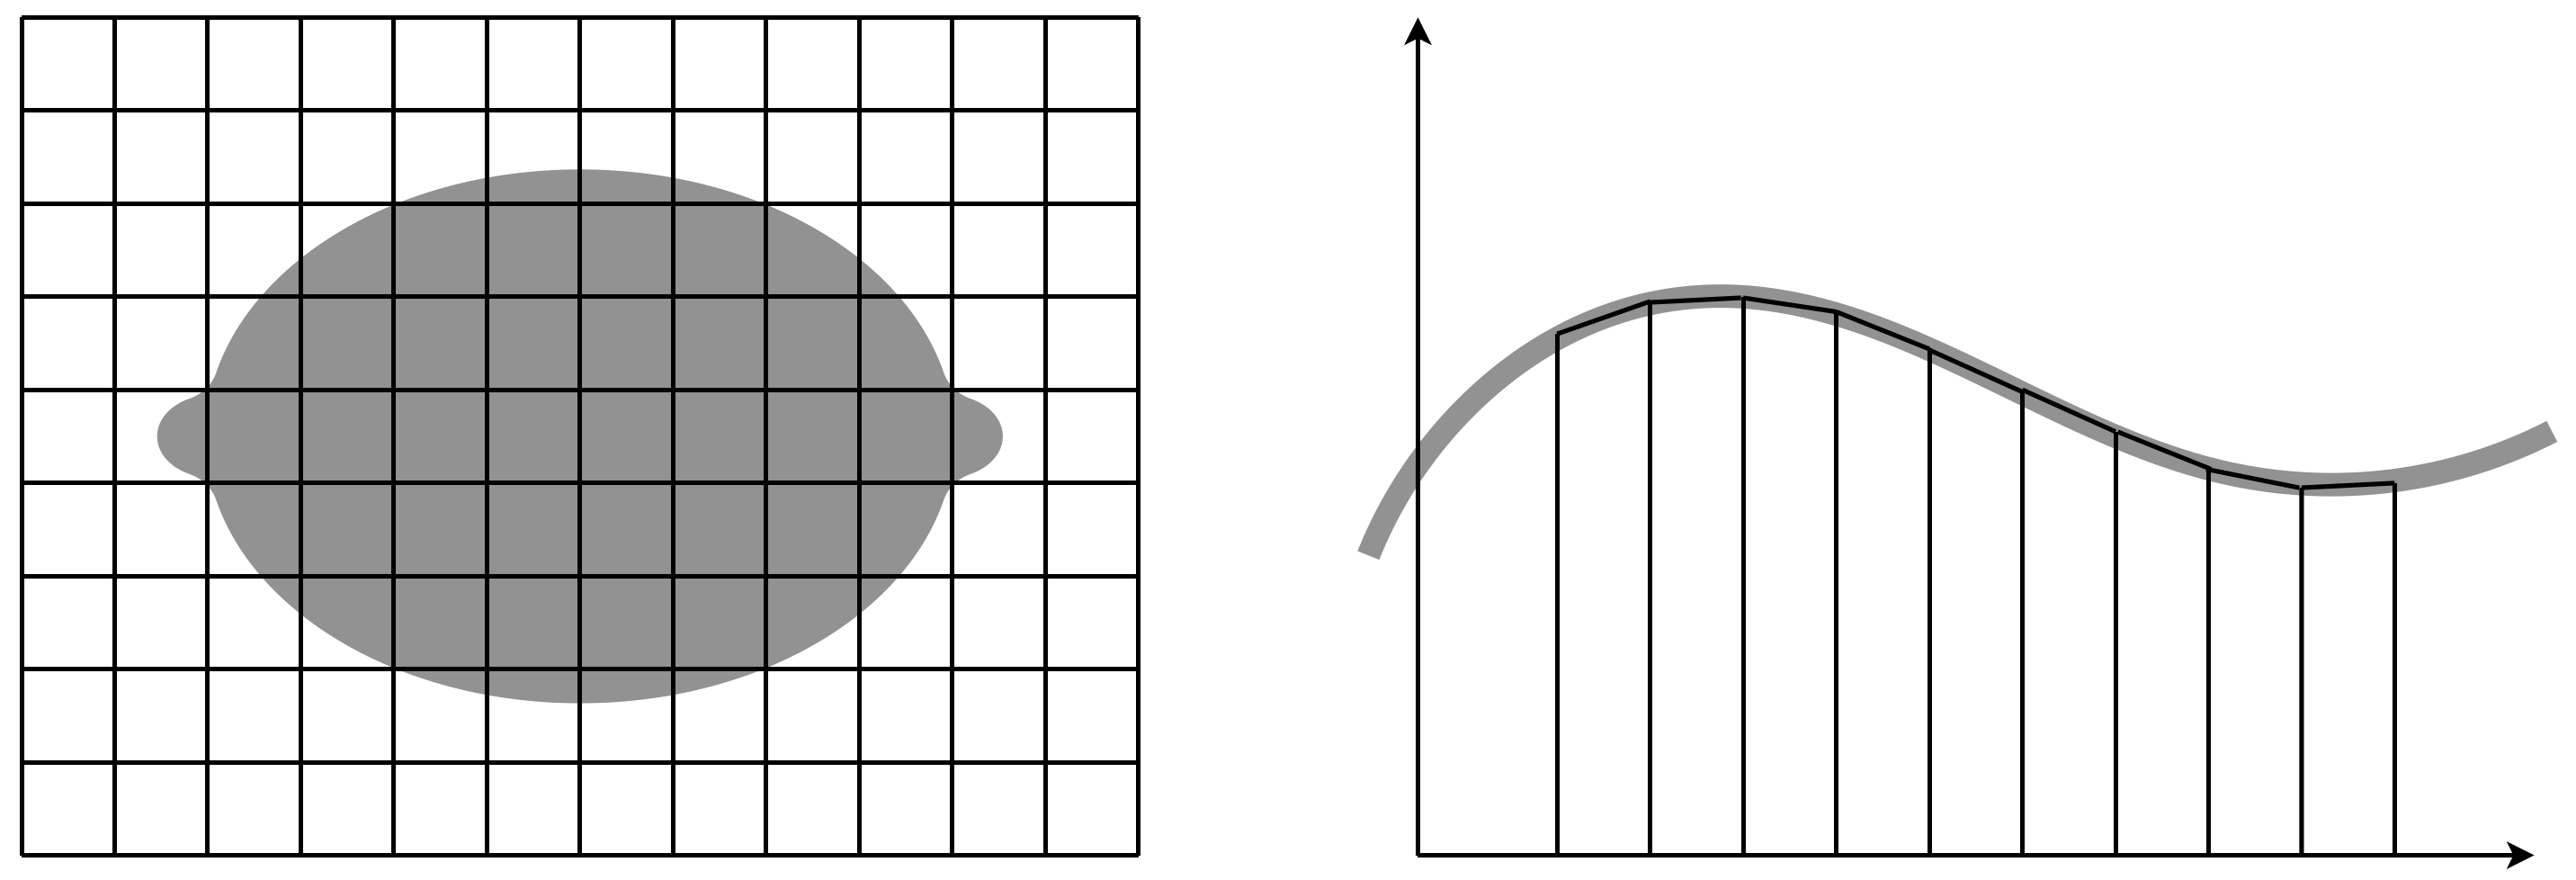
\includegraphics[width=0.75\linewidth]{pictures/2-Flaeche} 

}

\caption{Flächeninhaltsbestimmung}\label{fig:Flaeche}
\end{figure}

\hypertarget{fundamentale-ideen-nachbereitung}{%
\section{Zum Nachbereiten}\label{fundamentale-ideen-nachbereitung}}

\begin{enumerate}
\def\labelenumi{\arabic{enumi}.}
\tightlist
\item
  Lesen Sie das Kapitel 3.2.2 \emph{Der Begriff der Fundamentalen Ideen in der Pädagogik} bei Schubert \& Schwill (\protect\hyperlink{ref-Schubert:2011}{2011, S. 59--65}).
\item
  Wählen Sie ein Unterrichtsthema aus und stellen Sie den Bezug zu Fundamentalen Ideen her, indem Sie die \protect\hyperlink{tab:fragen-ebenen}{zugehörigen Fragen der semantischen Ebene} beantworten.
\end{enumerate}

\hypertarget{grundvorstellungen}{%
\chapter{Grundvorstellungen}\label{grundvorstellungen}}

\begin{quote}
\textbf{Ziele}

\begin{itemize}
\tightlist
\item
  Sie können die Grundvorstellungsidee beschreiben und wissen über deren Bedeutung für den Mathematikunterricht.
\item
  Sie kennen Grundvorstellungen zu einzelnen mathematischen Begriffen.
\end{itemize}

\textbf{Material}

\begin{itemize}
\tightlist
\item
  Folien zur Vorlesung zu Grundvorstellungen (\href{files/Stoffdidaktik-WiSe2223-Kap3.pdf}{pdf}, \href{files/Stoffdidaktik-WiSe2223-Kap3.key}{Keynote})
\end{itemize}
\end{quote}

\hypertarget{grundvorstellungen-begriffsklaerung}{%
\section{Begriffsklärung}\label{grundvorstellungen-begriffsklaerung}}

\hypertarget{grundvorstellungsidee}{%
\subsection{Grundvorstellungsidee}\label{grundvorstellungsidee}}

Als\index{Natürliche Zahlen|(} Sie zu Beginn Ihres Mathematikstudiums die Peano-Axiome zur Definition der Natürlichen Zahlen \(\mathbb{N}\) kennengelernt haben, konnten Sie dies wahrscheinlich -- trotz der Neuigkeit der formalen Beschreibung -- derart mit Ihrer Lebenswelterfahrung in Verbindung bringen, dass Natürliche Zahlen abgezählt werden können, also dass damit z.~B. die Platzierungen eines Wettrennens durchnummeriert werden können.

\begin{quote}
\textbf{Peano-Axiome} (\protect\hyperlink{ref-WikiPeano}{Wikipedia, 2021})

\begin{enumerate}
\def\labelenumi{\arabic{enumi}.}
\tightlist
\item
  \(0\) ist eine natürliche Zahl.
\item
  Jede natürliche Zahl \(n\) hat eine natürliche Zahl \(n'\) als Nachfolger.
\item
  \(0\) ist kein Nachfolger einer natürlichen Zahl.
\item
  Natürliche Zahlen mit gleichem Nachfolger sind gleich.
\item
  Enthält die Menge \(X\) die \(0\) und mit jeder natürlichen Zahl \(n\) auch deren Nachfolger \(n'\), so bilden die natürlichen Zahlen eine Teilmenge von \(X\).
\end{enumerate}
\end{quote}

Dieser \textbf{Bezug auf eine bekannte Handlung} ist wesentlich dafür, dass die Definition und damit der Begriff der Natürlichen Zahlen für Sie mit einem Sinn behaftet ist. Innerhalb dieser \emph{ordinalen Sichtweise} Natürlicher Zahlen helfen nun geeignete\footnote{\emph{Geeignet} heißt in diesem Fall, dass sich die Kernaussage des Begriffs in der Repräsentation wiederfindet. Im Ordinalzahlaspekt ist dies v.~a. die Reihung von Zahlen. Was dabei (noch) nicht relevant ist, ist zum Beispiel die exakte Messbarkeit, wie man sie etwa auf dem Zahlenstrahl repräsentiert.} \textbf{Repräsentationen} dabei, sich Rechenoperationen vorstellen und sie \textbf{operativ}\footnote{\emph{Operativ} heißt hier zum Beispiel, dass Sie zu einer Aufgabe wie \(2+7\) Nachbaraufgaben (\(2+8\)), Umkehraufgaben (\(7-2\)), Platzhalteraufgaben (\(2+\boxed{\phantom{5}}=7\)) usw. aufstellen und lösen können.} auszuführen zu können, also bspw. das Addieren als ein Weiterzählen aufzufassen (siehe Abbildung \ref{fig:Addition}).\index{Natürliche Zahlen|)}

\begin{figure}

{\centering 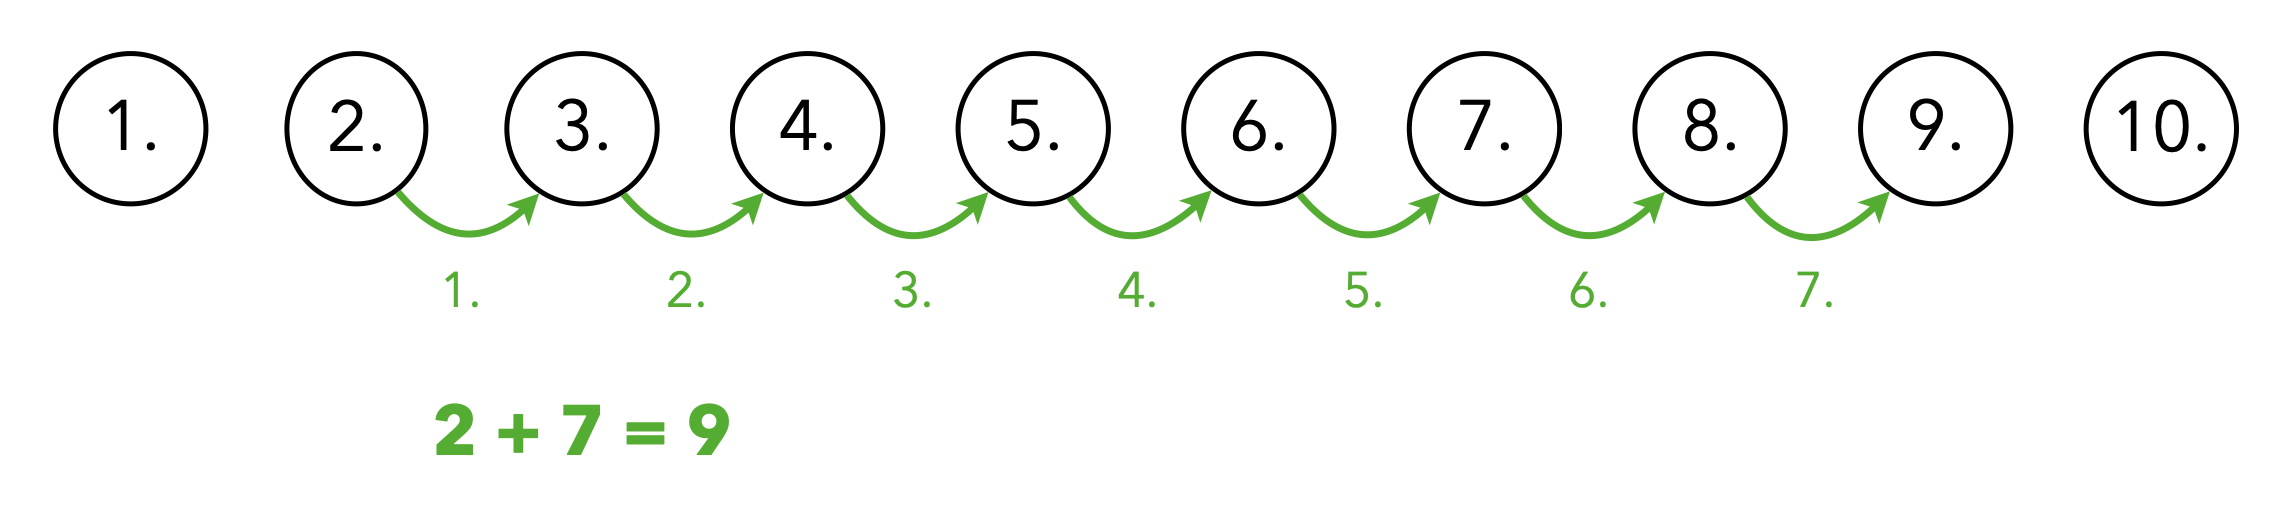
\includegraphics[width=0.75\linewidth]{pictures/3-Addition} 

}

\caption{Additionsaufgabe im ordinalen Zahlaspekt}\label{fig:Addition}
\end{figure}

Mit der Fähigkeit der Verknüpfung des mathematischen Begriffs und der Lebenswelt ist also eine \textbf{Anwendung des Begriffs auf die Wirklichkeit} möglich, insbesondere in Modellierungsprozessen. Dabei sind beide Richtungen relevant: Von der Realsituation zur Mathematik und von der Mathematik zur Realität.

Ziel des Mathematikunterrichts sollte es nun sein, für alle relevanten mathematischen Begriffe ein derartiges Verständnis aufzubauen, was auch heißt, verschiedene Vorstellungen zu einem Begriff zu vermitteln. Nach vom Hofe (\protect\hyperlink{ref-Hofe:1995}{1995, S. 97~f.}, Hervorhebung durch H.E.) ergibt sich daraus eine Orientierung an Grundvorstellungen im Mathematikunterricht:

\begin{definition}[Grundvorstellungen]
\protect\hypertarget{def:Grundvorstellungen}{}\label{def:Grundvorstellungen}

Die \textbf{Grundvorstellungsidee}\index{Grundvorstellung|textbf}\index{Grundvorstellungsidee|see{Grundvorstellung}} beschreibt \textbf{Beziehungen zwischen mathematischen Inhalten und} dem Phänomen der \textbf{individuellen Begriffsbildung}. In ihren unterschiedlichen Ausprägungen charakterisiert sie mit jeweils unterschiedlichen Schwerpunkten insbesondere drei Aspekte dieses Phänomens:

\begin{itemize}
\tightlist
\item
  Sinnkonstituierung eines Begriffs durch \textbf{Anknüpfung an} bekannte \textbf{Sach- oder Handlungszusammenhänge} bzw. \textbf{Handlungsvorstellungen},\index{Grundvorstellung!Sinnkonstituierung|textbf}
\item
  Aufbau entsprechender (visueller) \textbf{Repräsentationen bzw. »Verinnerlichungen«}, die \textbf{operatives Handeln} auf der Vorstellungsebene ermöglichen,\index{Grundvorstellung!Repräsentation|textbf}
\item
  Fähigkeit zur Anwendung eines Begriffs auf die Wirklichkeit durch \textbf{Erkennen der} entsprechenden \textbf{Struktur in Sachzusammenhängen} oder durch \textbf{Modellieren} des Sachproblems \textbf{mit Hilfe der mathematischen Struktur}.\index{Grundvorstellung!Modellierung|textbf}
\end{itemize}

\end{definition}

\hypertarget{ausdifferenzierung}{%
\subsection{Ausdifferenzierung}\label{ausdifferenzierung}}

Weiterhin unterscheidet vom Hofe (\protect\hyperlink{ref-vomHofe2014}{2014}) zwischen \textbf{primären}\index{Grundvorstellung!primäre Grundvorstellung} und \textbf{sekundären}\index{Grundvorstellung!sekundäre Grundvorstellung} Grundvorstellungen, abhängig von der Erfahrungswelt der Handlungen. Während sich primäre Grundvorstellungen auf reale Handlungserfahrungen stützen (z.~B. mit Steckwürfeln in der Arithmetik), entstammen sekundäre Grundvorstellungen aus den Handlungen mit bereits im Mathematikunterricht aufgebauten Repräsentationen (z.~B. Operationen auf dem Zahlenstrahl).

Ich als Autor dieses Dokuments vertrete die Ansicht, dass Grundvorstellungen zu \textbf{Aspekten} eines Begriffs und zu \textbf{Operationen} mit diesen Begriffsaspekten formuliert werden können. So wäre das oben angebrachte Beispiel der ordinalen Anordnung der Natürlichen Zahlen ein \emph{Begriffsaspekt} mit der damit verbunden Grundvorstellung, dass die Natürlichen Zahlen eine feste Reihenfolge darstellen, beginnend bei \(0\). Das \emph{Addieren} ist eine Operation in diesem Aspekt, verbunden mit der Grundvorstellung des Weiterzählens. Eine ähnliche Unterscheidung, jedoch mit inhaltlich anderer Ausrichtung, nehmen auch Greefrath et al. (\protect\hyperlink{ref-Greefrath2016}{2016, S. 17}) vor. Eine Diskussion dazu findet sich bei Etzold (\protect\hyperlink{ref-Etzold2021}{2021, S. 72~f.}). Die genannten Begriffs\emph{aspekte} sind jedoch nicht mit den \emph{Aspekten} der Grundvorstellungsidee in Definition \ref{def:Grundvorstellungen} zu verwechseln.
Auch wenn Sie nicht unmittelbar und sofort jeweils alle Aspekte eine Begriffs im Unterricht ansprechen werden, hilft Ihnen das Wissen über den Aspektreichtum in der Unterrichtsplanung für die Ausbildung eines umfassenden Begriffsverständnisses.

Die in Definition \ref{def:Grundvorstellungen} dargestellte Grundvorstellungsidee hat einen \textbf{normativen}\index{Grundvorstellung!normativ|textbf} Charakter, d.~h. es wird davon ausgegangen, dass (aus professioneller Sicht der Mathematikdidaktik) zu mathematischen Begriffen bestimmte Grundvorstellungen identifiziert werden können, die es im Unterricht zu vermitteln gilt. Oder anders gefragt: »Welche Grundvorstellungen sind zur Lösung des Problems aus der Sicht des Lehrenden adäquat?« (\protect\hyperlink{ref-Hofe:1995}{vom Hofe, 1995, S. 106}). Diese Sichtweise wird durch eine \textbf{deskriptive}\index{Grundvorstellung!deskriptiv|textbf} Perspektive ergänzt: »Welche individuellen Vorstellungen lassen sich im Lösungsversuch des Schülers erkennen?« (\protect\hyperlink{ref-Hofe:1995}{vom Hofe, 1995, S. 107}). Diese über empirische Untersuchungen zu ermittelnden Vorstellungen sind das, was sich Schülerinnen und Schüler \emph{tatsächlich} unter einem Begriff vorstellen, wozu ggf. auch typische \emph{Fehlvorstellungen}\footnote{Mit \emph{Fehlvorstellungen} sind hier individuelle Vorstellungen der Schülerinnen und Schüler gemeint, die mathematisch nicht tragfähig und daher aus fachlicher Perspektive fehlerhaft sind. So ist etwa die Vorstellung, dass Multiplizieren vervielfacht, in den Natürlichen Zahlen tragfähig (und damit eine Grundvorstellung), in den Bruchzahlen jedoch nicht mehr tragfähig und wird dort dann zur Fehlvorstellung. Neben \emph{Fehlvorstellungen} können weitere individuelle Vorstellungen \emph{Alltagsvorstellungen}, \emph{Präkonzepte} o.~ä. sein (siehe auch \protect\hyperlink{ref-Schecker2018}{Schecker et al., 2018, S. 11~f.}).} gehören können. Ein Wissen darüber ist für Lehrkräfte ungemein wichtig, um Ergebnisse von Schülerinnen und Schülern interpretieren und einordnen zu können und dann ggf. entsprechende Hilfsangebote zu machen. Dies entspricht dann einer \textbf{konstruktiven}\index{Grundvorstellung!konstruktiv|textbf} Perspektive auf Grundvorstellungen: »Worauf sind etwaige Divergenzen zurückzuführen, und wie lassen sich diese beheben?« (\protect\hyperlink{ref-Hofe:1995}{vom Hofe, 1995, S. 107}).

\hypertarget{gv-und-stoffdidaktik}{%
\section{GV und Stoffdidaktik}\label{gv-und-stoffdidaktik}}

Im Rahmen dieser Veranstaltung, insbesondere den von Ihnen ausgearbeiteten Seminarthemen, wird der Schwerpunkt auf \emph{normative} Grundvorstellungen gelegt, was der \textcolor{semanticColor}{semantischen Ebene} des \protect\hyperlink{tab:fragen-ebenen}{Vier-Ebenen-Ansatzes} zugeordnet werden kann, weil die mathematischen Begriffe hier mit einem Sinn versehen werden. Die \emph{deskriptive} und \emph{konstruktive} Perspektive sind dagegen der \textcolor{empiricColor}{empirischen Ebene} zuzuordnen, da hier individuelle Vorstellungen der Schülerinnen und Schüler von Relevanz sind. Dies betrifft insbesondere auch das Potenzial, (ggf. mathematisch unvollständige) individuelle Vorstellungen aufzugreifen bei der Ausbildung von (normativ erwünschten) Grundvorstellungen.

Das Identifizieren von Grundvorstellungen zu einem Begriff ist, genau wie bei den \protect\hyperlink{fundamentale-ideen}{Fundamentalen Ideen}, Aufgabe der mathematikdidaktischen Forschung (ein Modell dafür findet man bei \protect\hyperlink{ref-Salle2021}{Salle \& Clüver, 2021}). Als Lehrkraft profitieren Sie von diesen Ergebnissen und nutzen sie für Ihre stoffdidaktische Analyse.

Im Gegensatz zu den Fundamentalen Ideen, die ihren Ursprung in der Sachstruktur des mathematischen Inhalts haben, entstammen die Grundvorstellungen stärker der \emph{Bedeutung} der fachlichen Begriffe \emph{für das Individuum}. Grundvorstellungen beziehen sich auf spezifische Begriffe und Operationen mit Begriffen, während Fundamentale Ideen größere, themenübergreifende Leitlinien für die Stoffauswahl und -strukturierung bilden.

Für die Unterrichtsplanung und -durchführung ist neben der Frage, \emph{welche} Grundvorstellungen von Relevanz sind (Spezifizieren im Vier-Ebenen-Ansatz) vor allem interessant, \emph{wie} diese ausgebildet werden können (Strukturieren im Vier-Ebenen-Ansatz).

vom Hofe (\protect\hyperlink{ref-Hofe:1995}{1995, S. 123~ff.}) schlägt hierzu vor, zunächst aus Lehrkräftesicht den Lerngegenstand von der Mathematik her zu analysieren, Grundvorstellungen zu identifizieren, geeignete Sachzusammenhänge zu finden und diese mit den Erfahrungsbereichen der Schülerinnen und Schüler zu verknüpfen (linke Seite in Abbildung \ref{fig:GVausbilden}), während die Schülerinnen und Schüler dann den umgekehrten Weg zum Begriffserwerb gehen (rechte Seite in Abbildung \ref{fig:GVausbilden}).\index{Grundvorstellung!Aufbau von}



\begin{figure}

{\centering 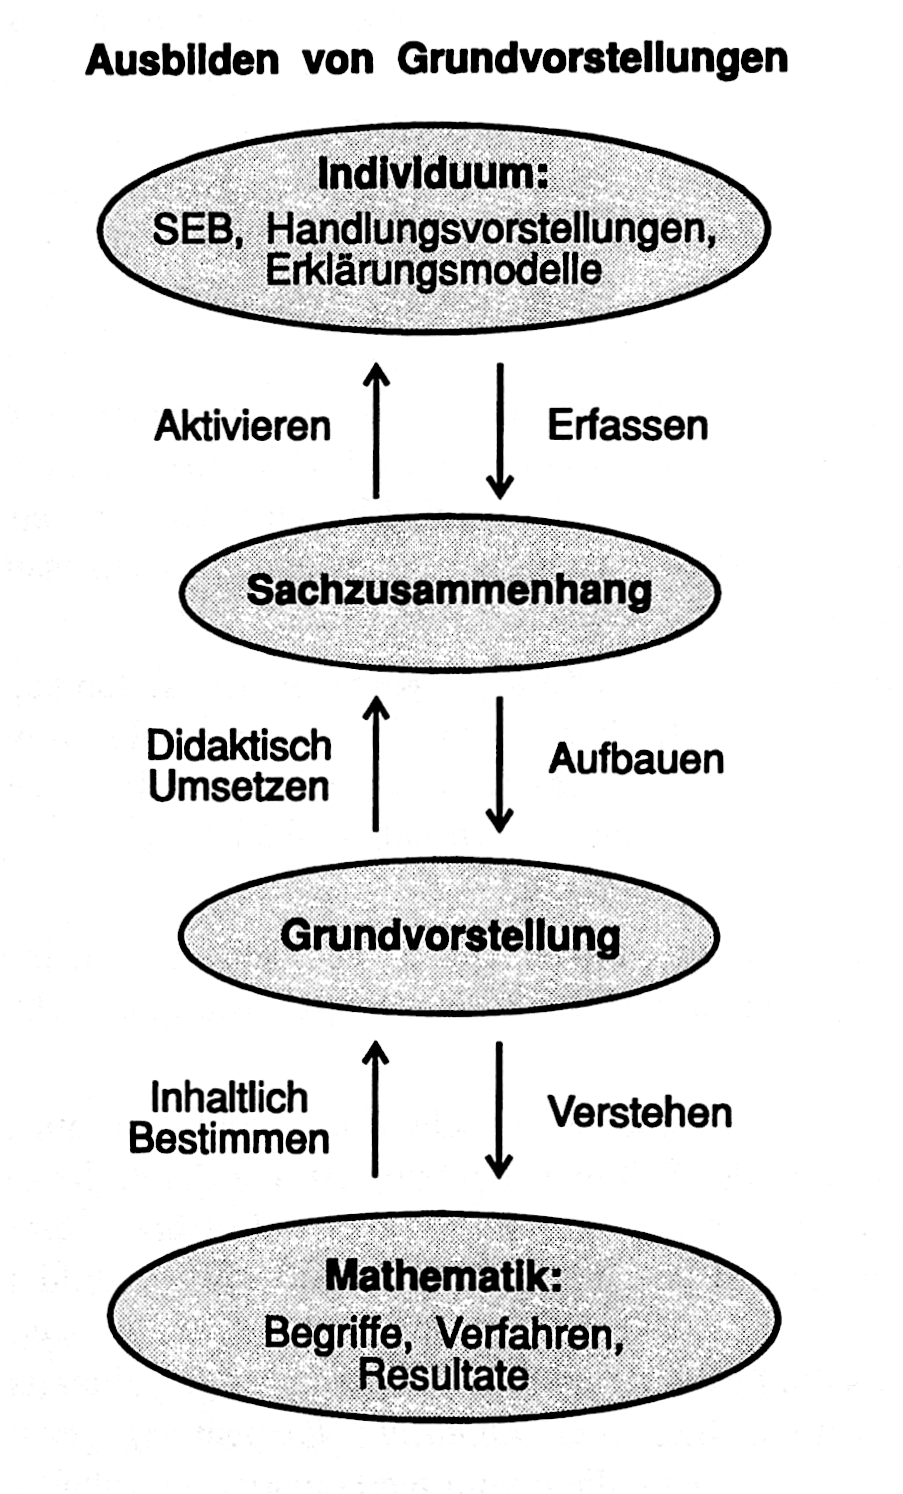
\includegraphics[width=0.5\linewidth]{pictures/3-GVausbilden} 

}

\caption{Ausbilden von Grundvorstellungen (\protect\hyperlink{ref-Hofe:1995}{vom Hofe, 1995, S. 124})}\label{fig:GVausbilden}
\end{figure}

Konkreter wird es an dieser Stelle jedoch noch nicht. Im Rahmen dieser Veranstaltung wird die Gestaltung von Lernprozessen in den Kapiteln \ref{lerntaetigkeit-und-lernhandlungen} bis \ref{aufgabengestaltung} in den Blick genommen, wo die Ausbildung von Grundvorstellungen noch einmal eine Rolle spielen wird.

\hypertarget{beispiele}{%
\section{Beispiele}\label{beispiele}}

\hypertarget{natuxfcrliche-zahlen}{%
\subsection{Natürliche Zahlen}\label{natuxfcrliche-zahlen}}

Betrachten Sie folgenden (fiktiven) Zeitungsartikel:\index{Natürliche Zahlen|(}

\begin{quote}
\textbf{\emph{Harlequin erneut auf dem 1. Platz}}

\emph{Bei dem traditionellen Pferderennen am 15. Mai hat das Pferd Harlequin erneut gewonnen. Unter den 10 Pferden, die an den Start gingen, belegte es mit 21,3 Sekunden den 1. Platz. Damit war es fast 2 mal so schnell unterwegs wie das letzte Pferd, das ins Ziel kam. Karten für das nächste Rennen können unter 030 23125143 bestellt werden.}
\end{quote}

In dem Text tauchen Zahlen unter vielen Aspekten auf: Der \textbf{1.} Platz und \textbf{15.} Mai sind \textbf{Ordinalzahlen}, also Zahlen, die eine Ordnung beschreiben. Wie oben schon beschrieben, lassen diese sich fachmathematisch über die Peano-Axiome beschreiben und wenn mit ihnen gerechnet, entspricht z.~B. das Addieren dem \textbf{Weiterzählen}.

Die \textbf{10} Pferde stellen eine \textbf{Kardinalzahl} dar, also die Anzahl der Elemente einer Menge. Addiert man Kardinalzahlen, so müssen \textbf{Mengen vereinigt} werden, z.~B. anschaulich, indem man sie zusammen legt.

Die \textbf{21,3} Sekunden entsprechen einer \textbf{Maßzahl}, da diese Zahl die Funktion hat, etwas auszumessen (hier die Zeit). Das Addieren in diesem Aspekt entspräche dem \textbf{Aneinanderlegen}, z.~B. wenn zwei Längenangaben addiert werden.

Dass es \textbf{2} mal so schnell wird, enspricht einem \textbf{Operatoraspekt}, mit dem die Vielfachheit eines Vorganges beschrieben wird. Das Addieren ist hierin eine \textbf{Hinereinanderausführung} eines Vorganges.

Die Telefonnumer \textbf{030 23125143} wiederum erfüllt einen \textbf{Codierungsaspekt}. Sie hat im mathematischen Sinne keine Bedeutung, nur die Anordnung der Ziffern ist von Relevanz. Entsprechend kann innerhalb dieses Aspektes auch nicht addiert werden. Weitere Beispiele hierfür wären Postleitzahlen oder Identifikationsnummern.

Hinzu kommt noch der Aspekt der \textbf{Rechenzahl}. Informationen dazu sowie eine genauere Erläuterung der Zahlaspekte und damit verbundenen Operationen findet man z.~B. bei Krauthausen (\protect\hyperlink{ref-Krauthausen:2018}{2018, S. 43~ff.}).\index{Natürliche Zahlen|)}

\hypertarget{bruchzahlen}{%
\subsection{Bruchzahlen}\label{bruchzahlen}}

Nachdem\index{Brüche|(} die Schülerinnen und Schüler ihr gesamte Vorschul- und Primarstufenzeit mit Natürlichen Zahlen verbracht haben, treten mit der Einführung von Bruchzahlen Umbrüche in den subjektiven Vorstellungen auf. Zum Beispiel sind folgende (vermeintlichen) Gesetzmäßigkeiten plötzlich \emph{nicht mehr} gültig:

\begin{itemize}
\tightlist
\item
  Das Produkt zweier Zahlen ist größer als die jeweiligen Faktoren.
\item
  Die Multiplikation kann als wiederholte Addition aufgefasst werden.
\item
  Jede Zahl hat genau einen Repräsentanten.
\item
  Je mehr Stellen eine Zahl hat, desto größer ist sie.
\end{itemize}

Die Bruchzahlen selbst besitzen nach Padberg \& Wartha (\protect\hyperlink{ref-Padberg:2017}{2017, S. 19~ff.}) folgende Aspekte:

\begin{itemize}
\tightlist
\item
  Bruch als \textbf{Anteil eines Ganzen} oder \textbf{mehrerer Ganzer}
  (z.~B. \(\frac{2}{3}\) als zwei Drittel einer Pizza oder je ein Drittel von zwei Pizzen),
\item
  Bruch als \textbf{Maßzahl}
  (z.~B. \(\frac{1}{4}\) Liter),
\item
  Bruch als \textbf{Operator}
  (z.~B. \(\frac{1}{5}\) von 250 €),
\item
  Bruch als \textbf{Verhältnis}
  (z.~B. \(\frac{2}{3}\) mit der Bedeutung \emph{2 von 3 Schüler/-innen tragen eine Brille}),
\item
  Bruch als \textbf{Quotient}
  (z.~B. \(\frac{3}{5}\) als Ergebnis bzw. andere Schreibweise von \(3:5\)),
\item
  Bruch als \textbf{Lösung einer linearen Gleichung}
  (z.~B. \(\frac{3}{5}\) als Lösung von \(5x = 3\)),
\item
  Bruch als \textbf{Skalenwert}
  (z.~B. \(\frac{3}{2}\) als Mitte zwischen \(1\) und \(2\) auf dem Zahlenstrahl),
\item
  \textbf{Quasikardinale Auffassung} von Brüchen
  (z.~B. \(\frac{3}{5}\) als 3 mal \(\frac{1}{5}\)).
\end{itemize}

Neben den Grundrechenoperationen führt auch das Vergleichen von Brüchen zu Grundvorstellungsumbrüchen. Hinzu kommen noch besondere Operationen mit Bruchzahlen wie das Erweitern und Kürzen.

Das Multiplizieren von Brüchen kann bspw. als Anteilsbildung (\(\frac{1}{5}\) mal \ldots{} heißt \(\frac{1}{5}\) \emph{von} \ldots) oder als Rechteckfläche aufgefasst werden (\protect\hyperlink{ref-Padberg:2017}{Padberg \& Wartha, 2017, S. 108~ff}), siehe Abbildung \ref{fig:Bruchmultiplikation}.

\begin{figure}

{\centering 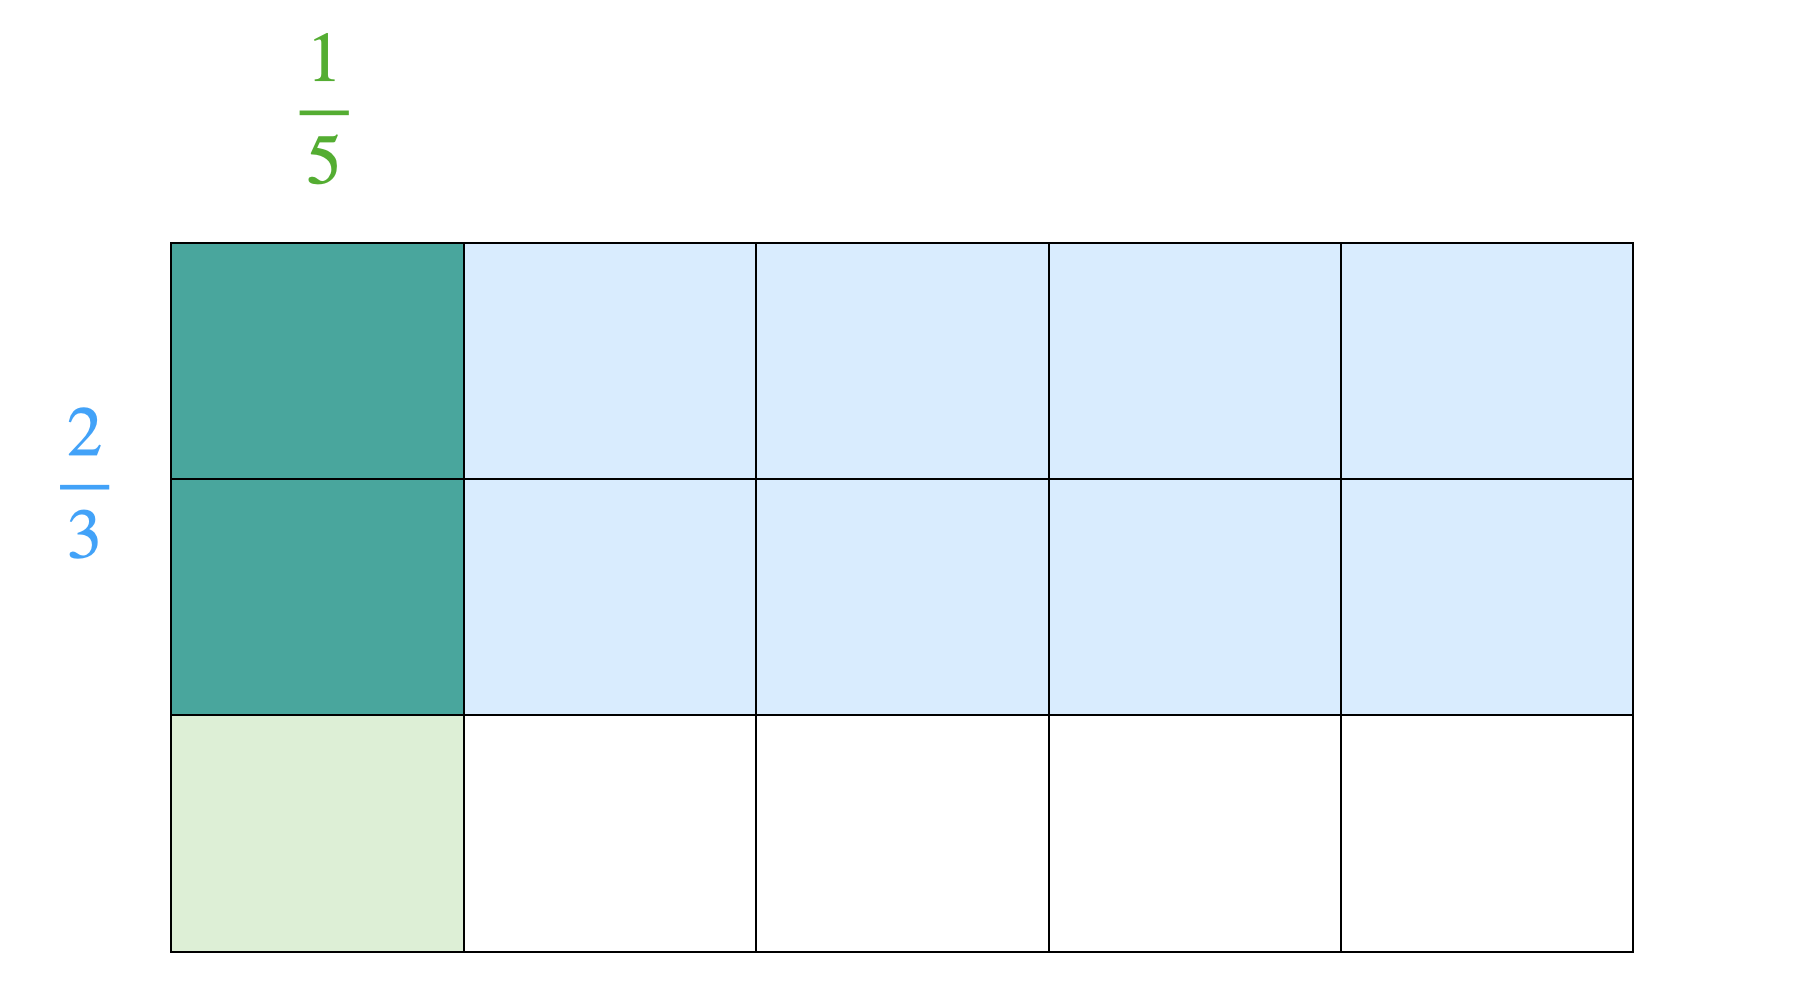
\includegraphics[width=0.5\linewidth]{pictures/3-Bruchmulti} 

}

\caption{Vorstellung von $\frac{1}{5} \cdot \frac{2}{3}$ als Rechteckfläche}\label{fig:Bruchmultiplikation}
\end{figure}

All dies zeigt, dass Brüche behutsam unterrichtet werden sollten und von einer rein kalkülorientierten Behandlung unbedingt abgesehen werden muss, da diese den nachhaltigen Lernerfolg deutlich mindert.\index{Brüche|)}

\hypertarget{grundvorstellungen-nachbereitung}{%
\section{Zum Nachbereiten}\label{grundvorstellungen-nachbereitung}}

\begin{enumerate}
\def\labelenumi{\arabic{enumi}.}
\tightlist
\item
  Lesen Sie (mindestens) die Kapitel 1.11.2, 1.11.4., 2.1, 2.2 und 2.4 des Buches \emph{Grundvorstellungen mathematischer Inhalte} (\protect\hyperlink{ref-Hofe:1995}{vom Hofe, 1995}).
\item
  Wählen Sie eine Grundvorstellung zu einem mathematischen Begriff aus und arbeiten Sie an dieser die Grundvorstellungsidee nach Definition \ref{def:Grundvorstellungen} durch, d.~h.

  \begin{itemize}
  \tightlist
  \item
    stellen Sie die Sinnhaftigkeit des Begriffs durch mögliche Handlungserfahrungen dar,
  \item
    finden Sie geeignete Repräsentationen, anhand derer operatives Handeln ermöglicht wird und
  \item
    beschreiben Sie mögliche Modellierungsprozesse des Begriffs mithilfe der gewählten Grundvorstellung.
  \end{itemize}
\item
  Wiederholen Sie Aufgabe 2 an weiteren Begriffen.
\end{enumerate}

\hypertarget{kernideen-kernfragen-kontexte}{%
\chapter{Kernideen, Kernfragen, Kontexte}\label{kernideen-kernfragen-kontexte}}

\begin{quote}
\textbf{Ziele}

\begin{itemize}
\tightlist
\item
  Sie können zu ausgewählten Lerngegenständen Kernideen und Kernfragen formulieren.
\item
  Sie können gegebene Kontexte zu Lerngegenständen hinsichtlich ihrer Sinnstiftung beurteilen.
\item
  Sie sind sich der Möglichkeiten und Bedeutung horizontaler und vertikaler Mathematisierung bewusst.
\end{itemize}

\textbf{Material}

\begin{itemize}
\tightlist
\item
  Folien zur Vorlesung zu Kernideen, Kernfragen und Kontexten (\href{files/Stoffdidaktik-WiSe2223-Kap4.pdf}{pdf}, \href{files/Stoffdidaktik-WiSe2223-Kap4.key}{Keynote})
\end{itemize}
\end{quote}

\hypertarget{kernidee-begriffsklaerung}{%
\section{Begriffsklärung Kernidee/-frage}\label{kernidee-begriffsklaerung}}

\textbf{Kernideen} haben die Aufgabe, den Lernpfad zu leiten und dabei \emph{sinnstiftend} das \emph{Wesen} des neuen Lerngegenstands sichtbar zu machen. Sie müssen dabei sowohl aus objektiver (also mathematischer) Perspektive tragfähig sein, als auch aus subjektiver Perspektive für die Schülerinnen und Schüler greifbar werden können. Kernideen bieten damit im \emph{Vorfeld} des Lernpfades eine Orientierung und im \emph{Nachgang} des Lernpfades eine Reflexionsmöglichkeit über den Lerngegenstand.\footnote{Der Begriff der Kernidee ist geprägt worden über das Dialogische Lernen nach Gallin und Ruf, spricht dort jedoch vorwiegend die Vorschauperspektive an (vgl. \protect\hyperlink{ref-Leuders2011}{Leuders et al., 2011, S. 7}).} Um bei den Schülerinnen und Schülern Lernprozesse zu einem Lerngegenstand zu initiieren, werden die Kernideen ansprechend in Form von \textbf{Kernfragen} formuliert. Kernfragen sollten daher prinzipiell aus subjektiver Sicht formuliert sein und insbesondere adressieren, wie man selbst mit dem Lerngegenstand umgehen kann.

Am Beispiel des \emph{Funktionsbegriffs}\index{Funktionsbegriff} etwa besteht eine Kernidee darin, dass Funktionen den Zusammenhang zwischen zwei Größen beschreiben und damit auch vorhersagen können (vgl. auch Aspekte des Funktionsbegriffs in Kapitel \ref{leitidee-strukturen-und-funktionaler-zusammenhang}). Als Kernfrage formuliert: »Wie kann man die Beziehung zwischen zwei sich verändernden Größen beschreiben und wie kann man damit weitere Werte bestimmen?« (\protect\hyperlink{ref-Thiel-Schneider2018}{Thiel-Schneider, 2018, S. 49}).

In der \emph{Vorschauperspektive} heißt das, die »Kernidee in Frageform schließt an individuelle Vorerfahrungen, Zielperspektiven, Denk- und Handlungsmuster der Lernenden an und initiiert die Auseinandersetzung mit dem mathematischen Gegenstand in den Worten von Schülerinnen und Schülern« (\protect\hyperlink{ref-Leuders2011}{Leuders et al., 2011, S. 8}). In der \emph{Rückschauperspektive} dagegen können über die Kernidee (dann quasi als Antwort auf die Kernfrage) »eine allgemeine Problemstellung und die zu ihrer Bewältigung notwendigen mathematischen Konzepte benannt« werden (\protect\hyperlink{ref-Leuders2011}{Leuders et al., 2011, S. 8}).

\begin{definition}[Kernidee und Kernfrage]
\protect\hypertarget{def:Kernidee}{}\label{def:Kernidee}Eine \textbf{Kernidee}\index{Kernidee|textbf} beschreibt unter sinnstiftender Perspektive das mathematische Wesen eines Lerngegenstands.

Eine \textbf{Kernfrage}\index{Kernfrage|textbf} stellt die Kernidee in Frageform aus der Perspektive der Schülerinnen und Schüler dar.

Kernideen und Kernfragen verfolgen eine \textbf{\emph{Vorschauperspektive}}\index{Kernidee!Vorschauperspektive|textbf}, die der Orientierung und Initiierung der Auseinandersetzung mit dem neuen Lerngegenstand dient, sowie eine \textbf{\emph{Rückschauperspektive}}\index{Kernidee!Rückschauperspektive|textbf}, die es den Schülerinnen und Schülern ermöglicht, den Lerngegenstand einzuordnen.
\end{definition}

Bestandteil Ihrer stoffdidaktischen Analyse auf der \textcolor{concreteColor}{konkreten Ebene} wird es also sein, zum Lerngegenstand passende Kernideen zu identifizieren und in Form von Kernfragen zu formulieren. Hierzu kann Ihnen die Sinnkonstituierung der jeweiligen Grundvorstellungen dienlich sein (siehe Definition \ref{def:Grundvorstellungen}).

\hypertarget{kontexte-begriffsklaerung}{%
\section{Begriffsklärung Kontext}\label{kontexte-begriffsklaerung}}

\textbf{Kontexte} sollen geeignet sein, sich dem Lerngegenstand exemplarisch zu nähern. Sie weisen damit immer eine Spezialisierung bzw. Konkretisierung des zu betrachtenden Lerngegenstands auf (denn nur so können die Schülerinnen und Schüler einen Zugang dazu finden) -- sollen aber so gestaltet sein, dass an Ihnen das Allgemeine erfahrbar ist (denn nur so kann es zu einer Beschäftigung mit der dahinterliegenden Mathematik kommen). Angelehnt an die Sinnstiftung der obigen Kernideen und Kernfragen, kann auch von einem \emph{sinnstiftenden Kontext} gesprochen werden.

Leuders et al. (\protect\hyperlink{ref-Leuders2011}{2011, S. 4}, Hervorhebungen im Original) formulieren hierzu:

\begin{definition}[Sinnstiftender Kontext]
\protect\hypertarget{def:Kontext}{}\label{def:Kontext}

Ein \textbf{sinnstiftender Kontext}\index{Kontext|textbf} ist ein Ausschnitt einer inner- oder außermathematischen Welt, der folgende Anforderungen möglichst gut erfüllt:

\begin{itemize}
\tightlist
\item
  Er ist anschlussfähig an die Erfahrungen, Interessen und die Denk- und Handlungsmuster der Lernenden \textbf{(Lebensweltbezug)}.\index{Kontext!Lebensweltbezug|textbf}
\item
  Er ermöglicht es, authentische Fragen zu bearbeiten und dabei auch etwas über den Kontext zu lernen \textbf{(Kontextauthentizität)}.\index{Kontext!Kontextauthentizität|textbf}
\item
  Er ist problemhaltig und offen genug, um Lernende zum reichhaltigen Fragen und Erkunden anzuregen \textbf{(Reichhaltigkeit)}.\index{Kontext!Reichhaltigkeit|textbf}
\end{itemize}

\end{definition}

Um einer eingeschränkten Sichtweise vorzubeugen, sei gesagt: Der \emph{Lebensweltbezug} heißt nicht zwingend, dass es sich um einen \emph{Realitätsbezug} (im Sinne einer Modellierung) handeln muss. Dies ist zwar in vielen Fällen angebracht, aber auch eine innermathematische Anschlussfähigkeit kann für die Schülerinnen und Schüler ansprechend sein (und damit Bezug zu deren -- schulischen -- Leben herstellen).

Ein möglicher Kontext, über den die oben formulierte Kernfrage bei \emph{linearen Funktionen}\index{Lineare Funktion}\index{Funktionsbegriff!Lineare Funktion|see{Lineare Funktion}} erarbeitet werden kann, wäre die Beschreibung des Abbrennverhaltens einer Kerze (vgl. \protect\hyperlink{ref-Boeer2014}{Böer et al., 2014, S. 108~f}). Dieser ist für die Schülerinnen und Schüler aus dem Alltag bekannt (wenn auch nicht alltäglich). Authentisch und reichhaltig ist der Kontext dahingehend, dass die meisten Kerzen zylinderförmig sind und daher tatsächlich ein lineares Abbrennverhalten haben. Auch ist es durchaus von Interesse, die Zeit bis zum vollständigen Abbrennen einer Kerze abschätzen zu können (z.~B. bei einer \emph{Kerzenuhr}, vgl. \protect\hyperlink{ref-WikiKerze}{Wikipedia, 2022}). Weiterhin können (später) die Eigenschaften des Funktionsgraphen kontextgebunden interpretiert werden (\(y\)-Achsenabschnitt als Ursprungslänge der Kerze, Nullstelle als die Zeit bis zum vollständigen Abbrennen, Anstieg des Graphen als Abbrennverhalten, das direkt mit der Dicke der Kerze in Verbindung gebracht werden kann).

Das Finden derartiger stinnstiftender Kontexte ist enorm anspruchsvoll! Sie sollten hier auf (gute) Lehrwerke zurückgreifen und immer wieder mögliche Kontexte kritisch (mithilfe der Definition \ref{def:Kontext}) hinterfragen.

Kernideen/Kernfragen und der sinnstiftende Kontext bilden damit eine Einheit in der Zielbildung und Motivation zu Beginn der Auseinandersetzung mit einem Lerngegenstand -- beides muss gemeinsam gedacht werden.

\hypertarget{mathematisierungstypen}{%
\section{Mathematisierungstypen}\label{mathematisierungstypen}}

Während Kernideen, Kernfragen und Kontexte in erster Linie der \emph{Spezifizierung} des Lerngegenstandes in Hinblick auf den Lernpfad dienen, kann zur \emph{Strukturierung} der Prozess der Mathematisierung stärker in den Blick genommen werden. Angelehnt an Treffers und Freudenthal stellt van den Heuvel-Panhuizen (\protect\hyperlink{ref-vandenHeuvel-Panhuizen2003}{2003, S. 12}) hierzu dar, dass prinzipiell zwei Wege der Mathematisierung möglich sind:

\begin{itemize}
\item
  Bei der \textbf{horizontalen Mathematisierung}\index{Horizontale Mathematisierung} werden mithilfe mathematischer Objekte und Operationen reale Situationen und alltägliche Probleme beschrieben, geordnet und gelöst. Es wird also aus der Welt des Lebens in die Welt der Symbole übergegangen.\footnote{im Original: »In the case of horizontal mathematizing, mathematical tools are brought forward and used to organize and solve a problem situated in daily life. {[}\ldots{]} to mathematize horizontally means to go from the world of life to the world of symbols« (\protect\hyperlink{ref-vandenHeuvel-Panhuizen2003}{van den Heuvel-Panhuizen, 2003, S. 12})}
\item
  Bei der \textbf{vertikalen Mathematisierung}\index{Vertikale Mathematisierung} wird innerhalb des mathematischen Systems reorganisiert und operiert, es wird sich also in der Welt der Symbole bewegt.\footnote{im Original: »Vertical mathematizing, on the contrary, stands for all kinds of re-organizations and operations done by the students within the mathematical system itself. {[}\ldots{]} to mathematize vertically means to move within the world of symbols« (\protect\hyperlink{ref-vandenHeuvel-Panhuizen2003}{van den Heuvel-Panhuizen, 2003, S. 12})}
\end{itemize}

Beide Arten sind nicht als Konkurrenten aufzufassen, sondern haben ihre gleiche Berechtigung im Mathematikunterricht. Dies ist v.~a. vor dem Hintergrund zu verstehen, dass Mathematik \emph{vom Menschen betrieben} wird. Erst durch das Zusammenwirken von horizontaler und vertikaler Mathematisierung kann Mathematik unter dieser Annahme auf ehrliche Weise durchgeführt und damit auch verstanden werden. Dies heißt insbesondere, dass in jeder Klassenstufe beide Arten der Mathematisierung ihre Berechtigung haben und entsprechend realisiert werden müssen.\footnote{im Original: »Freudenthal emphasized, however, that the differences between these two worlds are far from clear cut, and that, in his view, the worlds are not, in fact, separate. Moreover, he found the two forms of mathematizing to be of equal value, and stressed the fact that both activities could take place on all levels of mathematical activity.« (\protect\hyperlink{ref-vandenHeuvel-Panhuizen2003}{van den Heuvel-Panhuizen, 2003, S. 12})}

Das oben dargestellte Kerzenbeispiel entstammt der horizontalen Mathematisierung. Eine vertikale Mathematisierung könnte bspw. im weiteren Lernverlauf -- etwa nachdem die Funktionsgleichung \(y = m\cdot x + n\) eingeführt wurde -- die Untersuchung des Einflusses der Parameter \(m\) und \(n\) auf den Funktionsgraphen sein. Daran zeigt sich schon, wie hilfreich eine gleichermaßen Betrachtung horizontaler und vertikaler Prozesse ist, nämlich wenn etwa nach einer Veränderung von \(m\) und \(n\) rückgefragt wird, inwieweit dies noch mit den Abbrennen einer Kerze in Zusammenhang steht (was spätestens bei einem positiven \(m\) an seine Grenzen stößt). Derartige \emph{Grenzbetrachtungen} (die mathematisch greifbar sind, aber in der Realität eben an ihre Grenzen stoßen) bieten ein enormes Potenzial, sich dem abstrakten Wesen von Mathematik zu nähern.

\hypertarget{kernideen-kernfragen-kontexte-nachbereitung}{%
\section{Zum Nachbereiten}\label{kernideen-kernfragen-kontexte-nachbereitung}}

\begin{enumerate}
\def\labelenumi{\arabic{enumi}.}
\tightlist
\item
  Entwickeln Sie für den Begriff der \emph{Exponentialfunktion} eine Kernfrage.
\item
  Untersuchen Sie, inwieweit folgende Kontexte für Exponentialfunktionen sinnstiftend sind:

  \begin{itemize}
  \tightlist
  \item
    Bakterienwachstum
  \item
    Bierschaumzerfall
  \end{itemize}
\item
  Beschreiben und erklären Sie je eine geeignete Variante der horizontalen und vertikalen Mathematisierung am Lerngegenstand der Exponentialfunktion.
\end{enumerate}

\hypertarget{erstes-intermezzo-flaecheninhalt}{%
\chapter{Erstes Intermezzo: Flächeninhalt}\label{erstes-intermezzo-flaecheninhalt}}

\begin{quote}
\textbf{Ziele}

\begin{itemize}
\tightlist
\item
  Sie vertiefen Ihr Verständnis über den Vier-Ebenen-Ansatz, insbesondere auf der formalen, semantischen und konkreten Ebene.
\item
  Sie verknüpfen Ihr Wissen über Fundamentale Ideen, Grundvorstellungen, Kontexte und Kernideen/Kernfragen am Beispiel des Flächeninhaltsbegriffs.
\end{itemize}

\textbf{Material}

\begin{itemize}
\tightlist
\item
  Folien zur Vorlesung zum Ersten Intermezzo (\href{files/Stoffdidaktik-WiSe2223-Kap5.pdf}{pdf}, \href{files/Stoffdidaktik-WiSe2223-Kap5.key}{Keynote})
\end{itemize}
\end{quote}

In diesem Kapitel werden Fundamentale Ideen, Grundvorstellungen, Kernideen/Kernfragen und Kontexte im Zusammenhang mit dem Flächeninhaltsbegriff diskutiert. Ein Schulbuchkapitel zum Flächeninhaltsbegriff bietet die Motivation, die \textcolor{formalColor}{formale}, \textcolor{semanticColor}{semantische} und \textcolor{concreteColor}{konkrete} Ebene des \protect\hyperlink{tab:fragen-ebenen}{Vier-Ebenen-Ansatzes} zu diskutieren und einen ersten Ausblick auf die \textcolor{empiricColor}{empirische} Ebene zu geben.

In dem Sinne wird also existierendes Material analysiert und hinsichtlich der mathematikdidaktischen Theorie reflektiert. Ein solches Vorgehen wäre auch für Ihren Seminarvortrag bzw. die Hausarbeit im Rahmen dieser Veranstaltung möglich -- dann natürlich etwas ausführlicher, als hier dargestellt.

\hypertarget{darstellung-im-schulbuch}{%
\section{Darstellung im Schulbuch}\label{darstellung-im-schulbuch}}

In dem Schulbuch \emph{Mathewerkstatt} (\protect\hyperlink{ref-Barzel2012}{Barzel et al., 2012c}) wird der Flächeninhalt über den Kontext von Tiergehen eingeführt (siehe Abbildung \ref{fig:Tiergehege}). So haben in einem Zoo verschiedene Tiere unterschiedlich große Gehe zur Verfügung. Die Form der Gehege variiert dabei ebenfalls.



\begin{figure}

{\centering 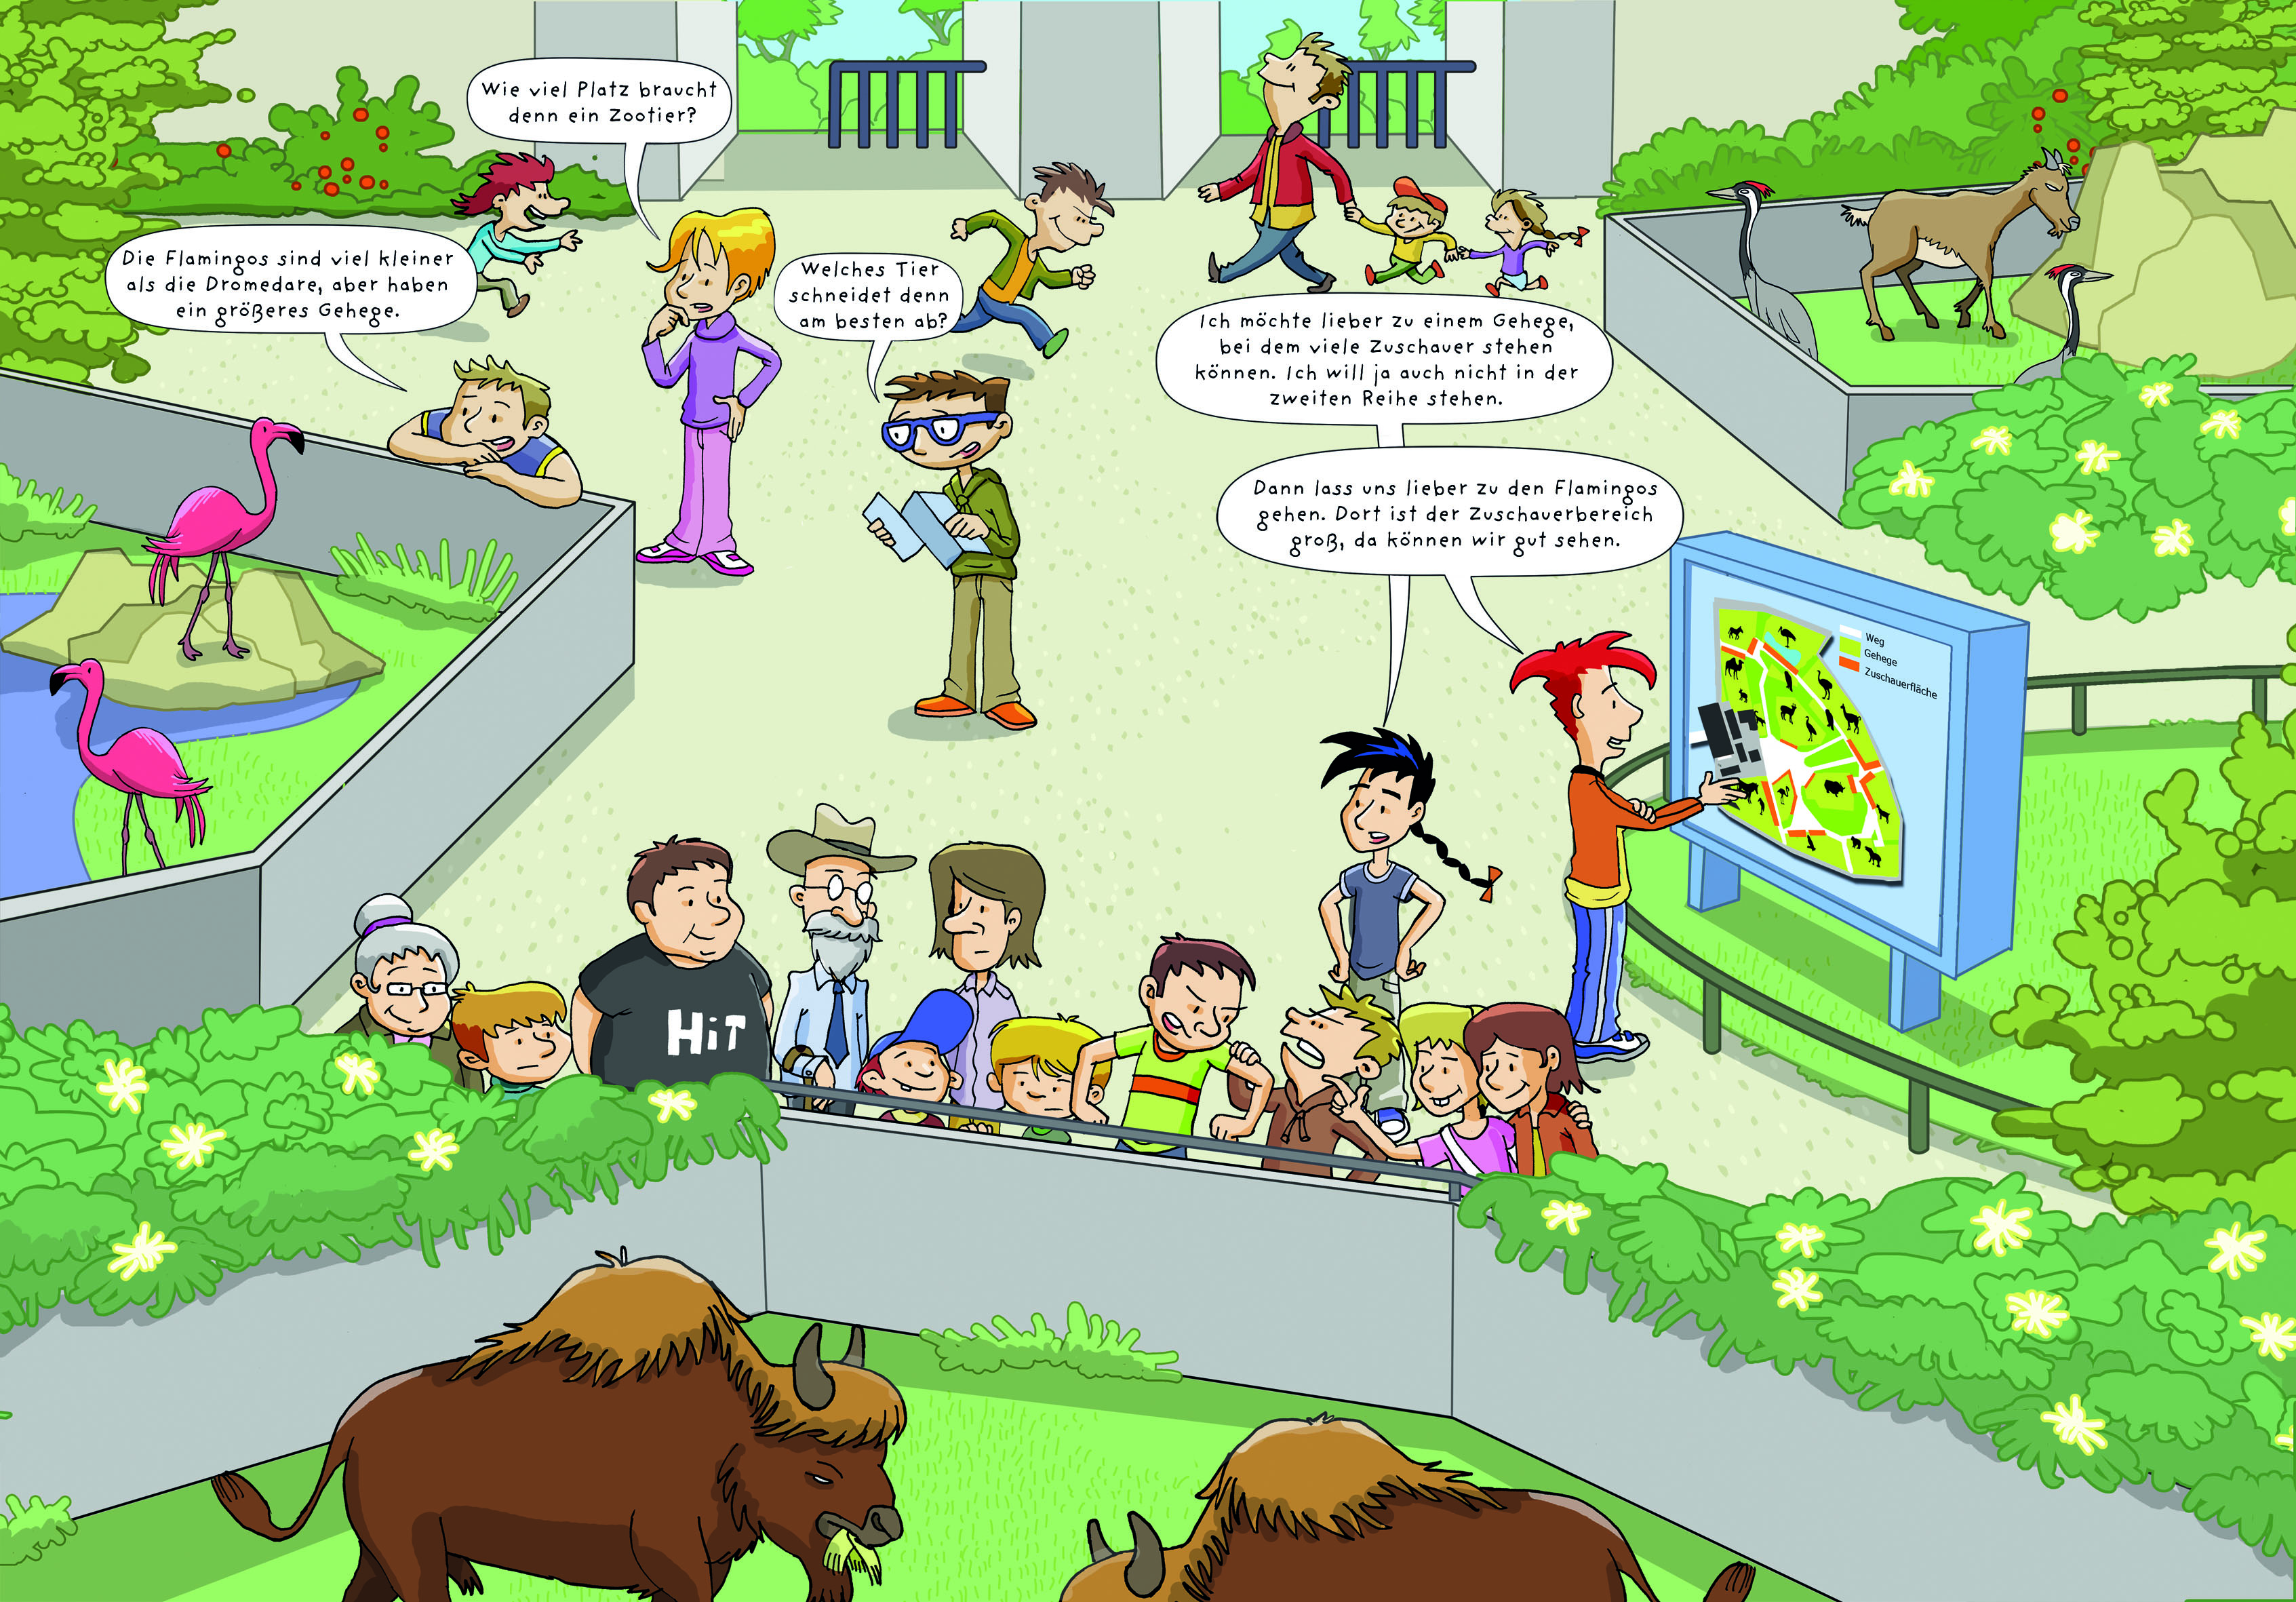
\includegraphics[width=1\linewidth]{pictures/5-Tiergehege} 

}

\caption{Einstiegsbild zum Thema Flächeninhalt (\protect\hyperlink{ref-Barzel2012}{Barzel et al., 2012c, S. 168~f.})}\label{fig:Tiergehege}
\end{figure}

Die Schülerinnen und Schüler werden nun in einer Erkundungsphase vor die Aufgabe gestellt, die Gehegegrößen miteinander zu vergleichen sowie möglichst geschickt die Größe eines Geheges messen zu können.

Anschließend erfolgen Ordnungs- und Vertiefungsphasen, in denen das Wissen struktruiert und geübt wird. Das Schulbuch wird durch einen Materialblock begleitet (\protect\hyperlink{ref-Barzel2012b}{Barzel et al., 2012b}), was in diesem Fall insbesondere dem Auseinanderschneiden und Zusammenlegen bzw. dem Auslegen von Flächen dienen soll. Weiterhin gibt es für Lehrerinnen und Lehrer ein ausführliches Begleitmaterial (\protect\hyperlink{ref-Barzel2012a}{Barzel et al., 2012a}), in dem alle Seiten des Schulbuches sowie fachdidaktische Hintergründe zur Thematik erläutert sind.

\hypertarget{formale-ebene-1}{%
\section{Formale Ebene}\label{formale-ebene-1}}

\begin{quote}
Welche Begriffe und Sätze sollen erarbeitet werden?
Welche Verfahren sollen erarbeitet werden und wie werden sie formal begründet?
Wie lassen sich die Begriffe, Sätze, Begründungen und Verfahren logisch strukturieren?
Welche Verbindungen zwischen den Fachinhalten sind entscheidend, welche weniger bedeutsam?
Wie kann das Netzwerk aus Begriffen, Sätzen, Begründungen und Verfahren entwickelt werden?
\end{quote}

Fachmathematisch kann der Flächeninhalt einer Figur als ein \textbf{nichtnegatives Maß} aufgefasst werden, wobei zwei \textbf{zueinander kongruenten Figuren dasselbe Maß} zugeordnet wird und der Flächeninhalt einer Figur gleich der \textbf{Summe der Flächeninhalte ihrer Teilfiguren} ist, sofern zerlegbar. Hinzu wird das Flächeninhaltsmaß eines Quadrates der Seitenlänge 1~LE auf 1~LE2 festgelegt (vgl. \protect\hyperlink{ref-Kuntze2018}{Kuntze, 2018, S. 161}).

Dies ist eine \textbf{axiomatische Herangehensweise}, die sich für Schülerinnen und Schüler in der Regel als herausfordernd darstellt (\protect\hyperlink{ref-Kuntze2018}{Kuntze, 2018, S. 162}). Häufig wird eine umschreibende Definition genutzt, wie: \emph{Der Flächeninhalt einer Fläche gibt an, wie groß diese ist.} Dabei ist jedoch die mögliche Mehrdeutigkeit dieser Formulierung zu beachten -- so könnte auch der Umfang einer Figur als Maß für ihre \emph{Größe} aufgefasst werden, da der Größenbegriff in dem Fall unspezifisch ist.

Ob nun eine explizite Definition gewählt wird oder nicht -- dies ist auch abhängig von der persönlichen Einstellung der Lehrkraft und den Voraussetzungen der Lerngruppe -- in jedem Fall ist ein tragfähiges mathematisches Verständnis aufzubauen. Hierzu können die in den Axiomen enthaltenen Eigenschaften über sinnvolle \textbf{Lernhandlungen} aufgebaut werden (siehe auch \protect\hyperlink{ref-Worner2014}{Wörner, 2014, S. 1328~f.}):

\begin{itemize}
\tightlist
\item
  Vergleichen verschiedener Flächen durch Zerlegen, Ergänzen und Übereinanderlegen
\item
  Bestimmen des Maßes einer Fläche über Auszählen mittels eines Vergleichsmaßes
\item
  Nutzen eines quadratischen Vergleichsmaßes, in der Regel 1~cm2
\end{itemize}

All diese Überlegungen kommen zunächst \textbf{ohne Formeln} aus, weshalb diese im Unterricht auch erst im Anschluss an eine inhaltliche Erarbeitung des Flächeninhaltsbegriffs eingeführt und genutzt werden sollten.

Fachsystematisch entscheidend ist, dass ein \textbf{Flächenvergleich zunächst ohne ein explizites Maß} möglich ist -- hierfür reichen die Kongruenzeigenschaft und das Zerlegen/Ergänzen von Flächen aus. Das Vergleichsmaß ist dann relevant, wenn man den \textbf{Flächeninhalt mithilfe einer Zahl objektivieren} bzw. ohne eine explizite Vergleichsfigur auskommen möchte.

Interessant ist hier auch die \textbf{\emph{Willkürlichkeit} des Vergleichsmaßes}. Kulturell geprägt ist hier (in Kontinentaleuropa) zwar beispielsweise 1~cm2, aber auch andere Einheiten sind gleichberechtigt möglich. Auch muss das Vergleichsmaß nicht zwingend ein Quadrat sein. Nicht selten wird z.~B. von großen Flächen angegeben, wie viele Fußballfelder in sie hineinpassen würden. Für den Unterricht bedeutet das, dass im Sinne einer auf den mathematischen Kern orientierten Sichtweise zunächst möglichst allgemeine und vielfältige (auch \emph{unförmige}) Vergleichsflächen herangezogen werden können. Später ist dann natürlich ein Bezug zu den Standardeinheiten herzustellen (siehe Abbildung \ref{fig:FlaecheEinheiten}).



\begin{figure}

{\centering 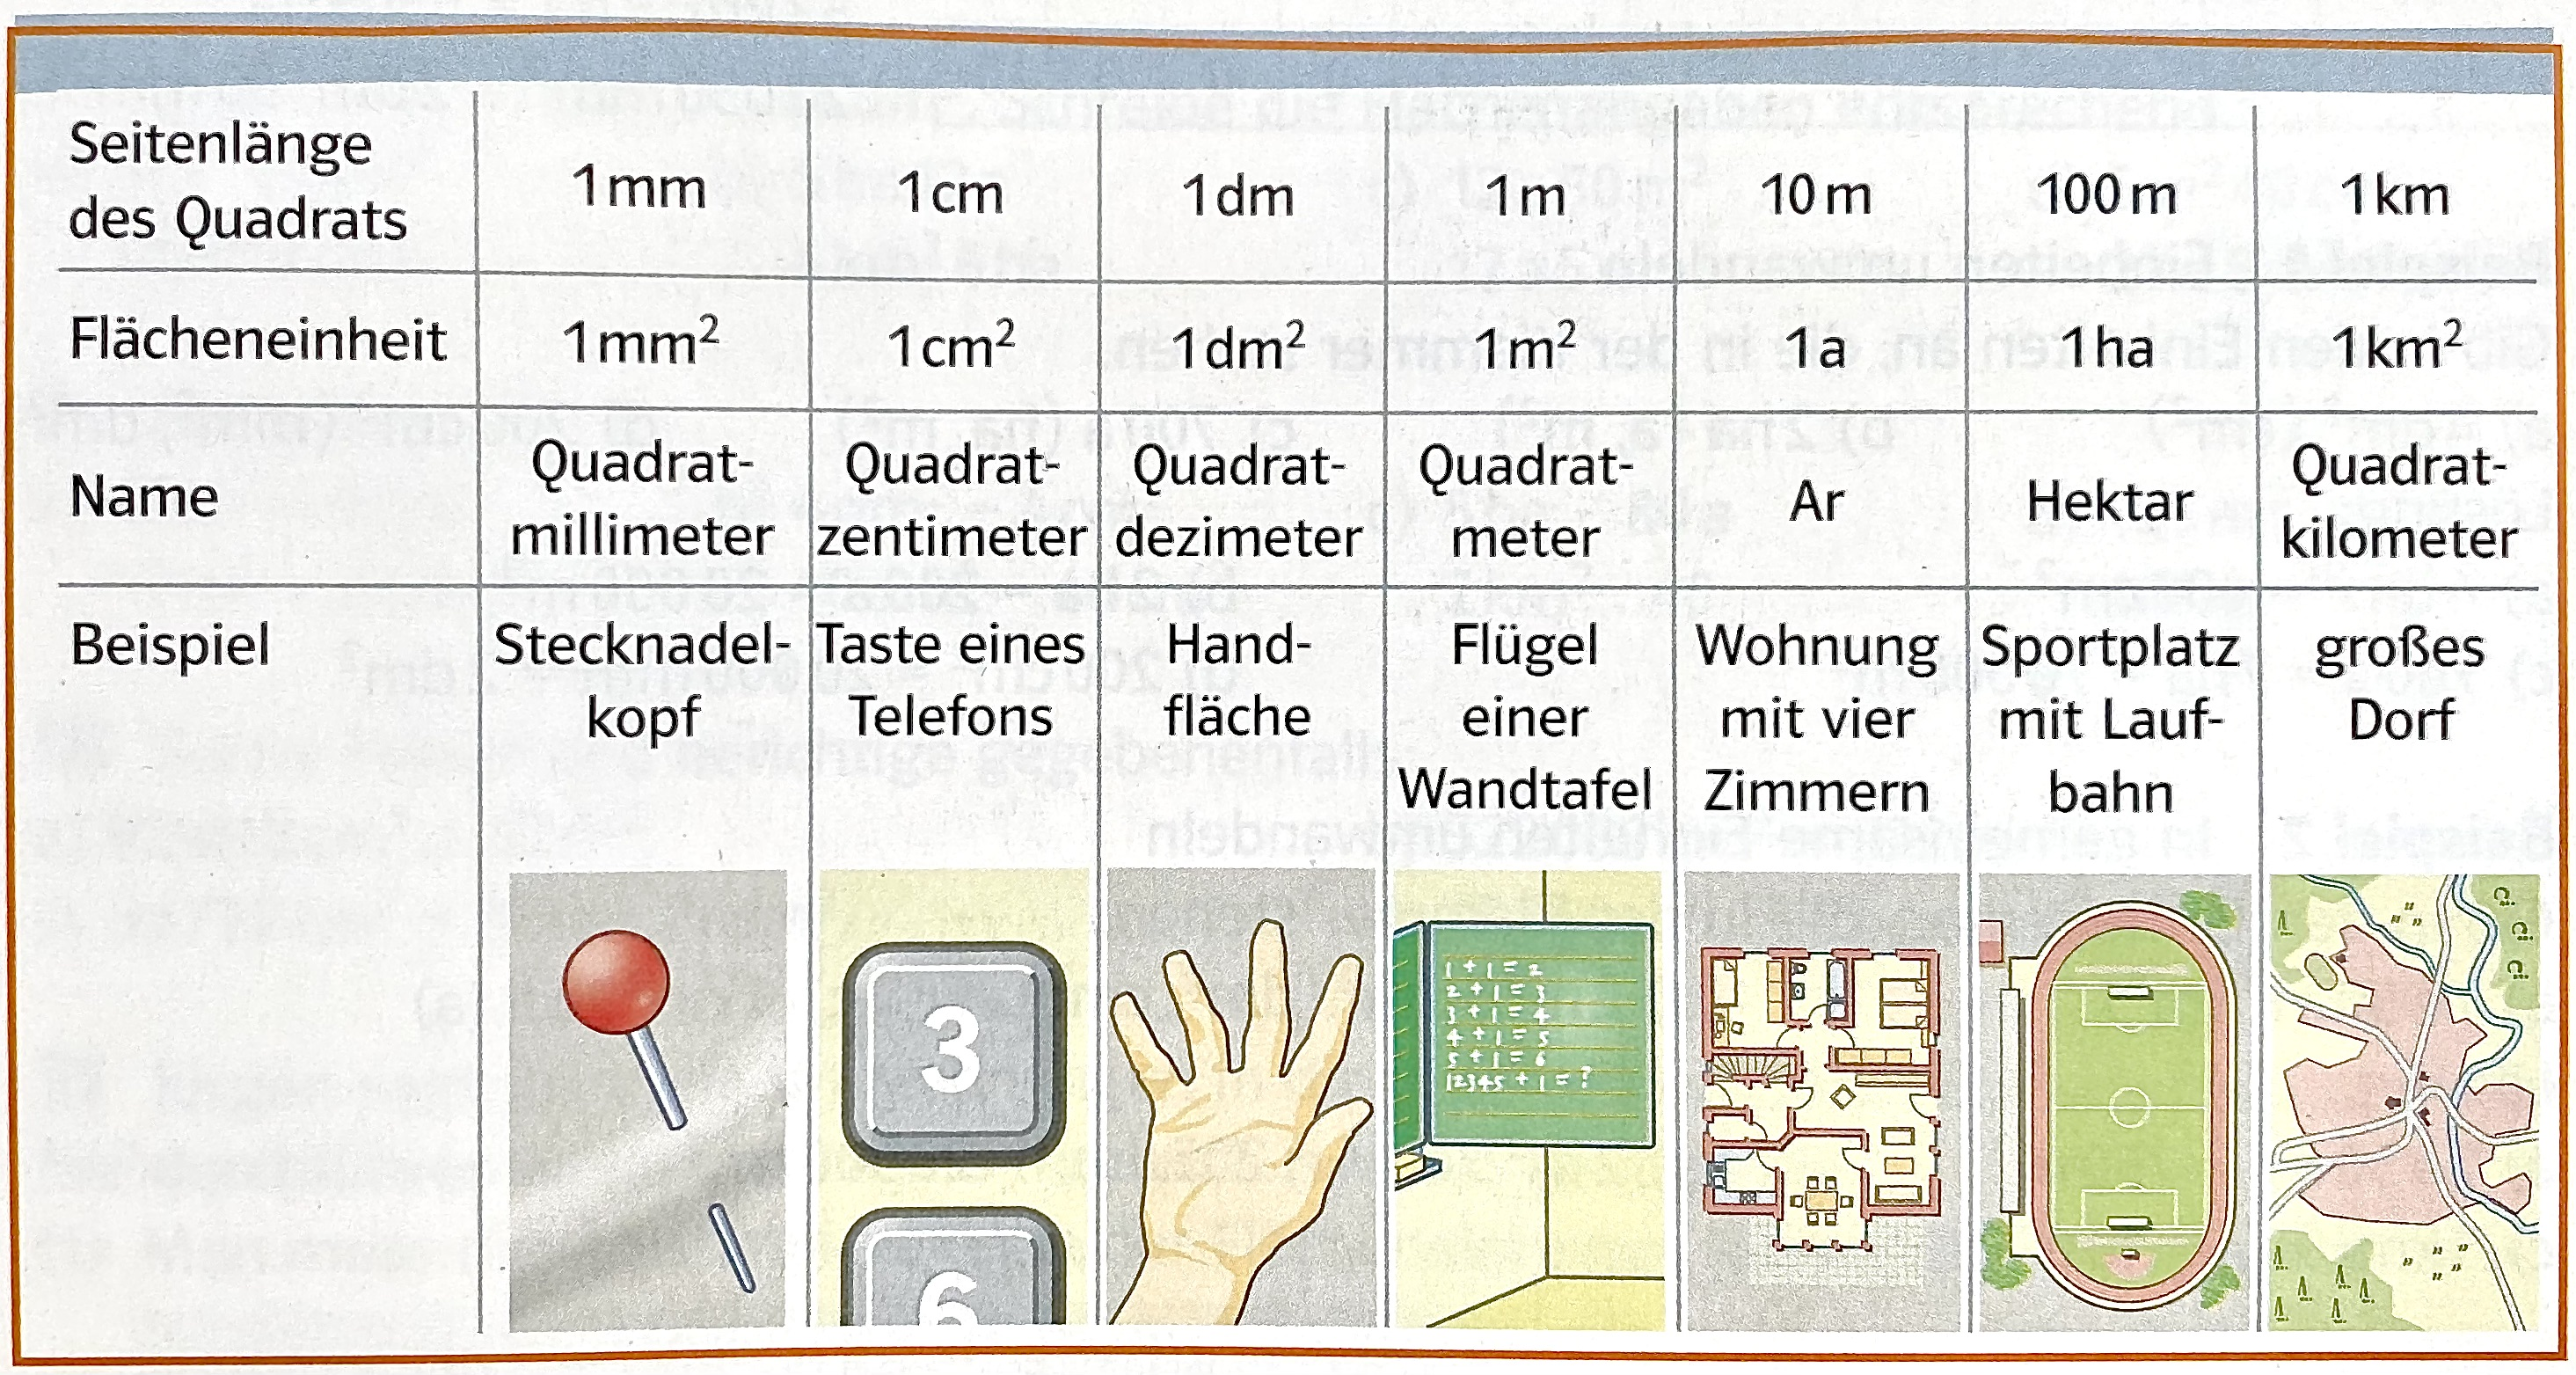
\includegraphics[width=0.75\linewidth]{pictures/5-Einheiten} 

}

\caption{Standardeinheiten typischer Vergleichsflächen (\protect\hyperlink{ref-Lambacher2010}{\emph{Lambacher {Schweizer} {Mathematik} für {Gymnasien}. 5, {Schülerbuch}}, 2010, S. 193})}\label{fig:FlaecheEinheiten}
\end{figure}

\hypertarget{semantische-ebene-1}{%
\section{Semantische Ebene}\label{semantische-ebene-1}}

\begin{quote}
Welche Fundamentalen Ideen liegen hinter den Begriffen, Sätzen und Verfahren?
Welche Grundvorstellungen und Repräsentationen (graphisch, verbal, numerisch und algebraisch) sind für den Verständnisaufbau entscheidend?
Wie verhalten sich Ideen und Vorstellungen zueinander und zu früheren und späteren Lerninhalten?
Wie kann ein Lernpfad angeordnet werden, in dem das Verständnis, zusammen mit den Erkenntnissen der formalen Ebene, aufgebaut wird?
\end{quote}

\hypertarget{fundamentale-idee-messen}{%
\subsection{Fundamentale Idee Messen}\label{fundamentale-idee-messen}}

Dem Flächeninhaltsbegriff liegt zweifelsohne die Fundamentale Idee des \emph{Messens} zugrunde. Vohns (\protect\hyperlink{ref-Vohns:2000}{2000, S. 52~ff.}) stellt ausführlich dar, warum das Messen als Fundamentale Idee aufgefasst werden kann, worauf in diesem Abschnitt Bezug genommen wird. Besondere Betonung legt Vohns (\protect\hyperlink{ref-Vohns:2000}{2000, S. 49}) darauf, dass Messen »der indirekte Vergleich von Objekten in bezug {[}sic{]} auf eine bestimmte Eigenschaft« ist.

\emph{Horizontal} zieht sich dies über viele Gebiete der Mathematik hinweg (z.~B. Messprozesse in der Geometrie, Maßzahlaspekt von Brüchen in der Arithmetik, Erwartungswert als Lagemaß in der Stochastik, Integral in der Analysis), aber auch darüber hinaus ist das Messen von hoher Relevanz (z.~B. Messprozesse in der Physik, quantitative Studien in den Sozialwissenschaften, Pulsmessung in der Medizin). Damit wird auch das \emph{Sinnkriterium} der Fundamentalen Idee offensichtlich.

Das \emph{Vertikalkriterium} zeigt sich beispielsweise in der Längenbestimmung in der Grundschule, Flächeninhaltsbestimmung in der Orientierungsstufe, bei Verwandlungen von Flächen (z.~B. beim Beweis des Satzes des Pythagoras) bzw. der Approximation von Flächen (z.~B. Bestimmen des Kreisflächeninhalts) bis hin zum Integralbegriff als verallgemeinerter Flächeninhalt.

\emph{Historisch} ist das Messen ebenfalls in vielen Epochen der Mathematik bedeutsam, worauf typische Wortwendungen wie \emph{Alles ist Zahl!} (bei den Pythagoräern), \emph{Die Vermessung der Welt} (mit der Methode der Triangulation) oder die \emph{Quadratur des Kreises} (als klassisches Problem der Geometrie) hindeuten. Auch die Vereinheitlichung von Maßeinheiten (z.~B. SI-Einheiten) zeigt die Bedeutsamkeit des Messens für die wissenschaftliche Entwicklung.

\hypertarget{gv-zum-fluxe4cheninhalt}{%
\subsection{GV zum Flächeninhalt}\label{gv-zum-fluxe4cheninhalt}}

Die folgenden Überlegungen sind empirisch nicht abgesichert, sondern vorwiegend theoretischer Natur. Ansatzpunkt ist ein Beitrag von Wörner (\protect\hyperlink{ref-Worner2014}{2014}). Setzt man die dortigen Darstellungen genauer mit der Definition \ref{def:Grundvorstellungen} von Grundvorstellungen in Bezug, lassen sich (meiner Meinung nach) Grundvorstellungen zu drei Aspekten des Flächeninhaltsbegriffs formulieren:

\begin{itemize}
\tightlist
\item
  \textbf{Maßzahlaspekt}: Flächeninhalt einer Figur als nichtnegative Maßzahl, die mittels normierter Flächeninhaltsmaße bestimmt wird
\item
  \textbf{Vereinigungsaspekt}: Flächeninhalt einer Figur als Summe der Flächeninhalte der Teilfiguren, aus denen sich die Figur zusammensetzen lässt
\item
  \textbf{Kongruenzaspekt}: Flächeninhalt einer Figur als invariante Eigenschaft gegenüber Kongruenzabbildungen
\end{itemize}

Für jeden dieser Aspekte sollen nun Handlungserfahrungen, Repräsentationen und mögliche Anwendungen auf die Realität diskutiert werden. Weiterhin werden einige Operationen mit Flächeninhalten besprochen.

\hypertarget{mauxdfzahlaspekt}{%
\subsubsection{Maßzahlaspekt}\label{mauxdfzahlaspekt}}

Eine Erfahrung, die die Grundvorstellung zu diesem Aspekt stützt, ist das Auslegen von Flächen mittels normierter Flächenstücke, wie z.~B. Quadrate. Hieraus kann die Erfahrung gewonnen werden, dass die Anzahl der Quadrate direkt den Flächeninhalt (mit der entsprechenden Einheit) angibt.

Als Repräsentation kann hierfür einfaches Kästchenpapier dienen, auf das die auszumessende Fläche gemalt wird (siehe Abbildung \ref{fig:FlaecheMasszahl}). Daran kann man das Abzählen der normierten Flächenstücke durchführen bzw. sich vorstellen. Insbesondere können daran auch Verfeinerungen (und damit genaueres Messen) nachvollzogen werden.

\begin{figure}

{\centering 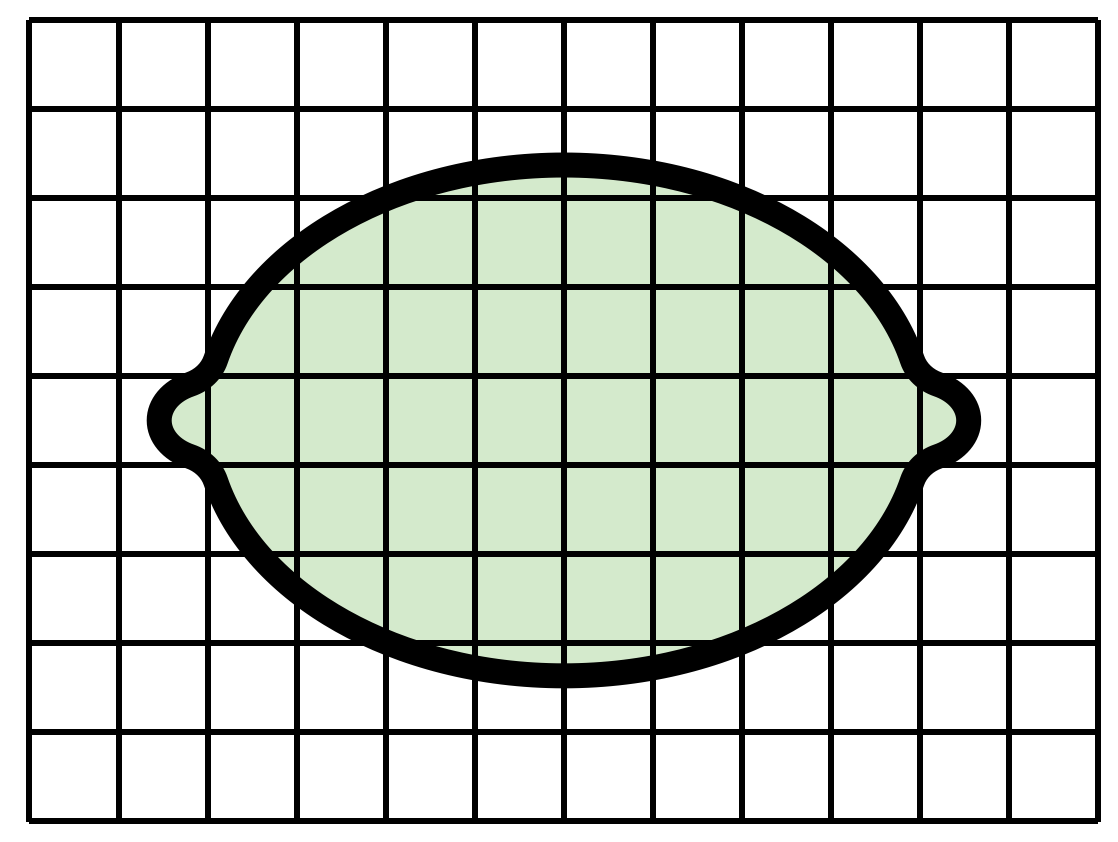
\includegraphics[width=0.25\linewidth]{pictures/5-Masszahl} 

}

\caption{Repräsentation des Maßzahlaspektes}\label{fig:FlaecheMasszahl}
\end{figure}

Eine mögliche Anwendung in der Realität ist das Bestimmen der Größe eines Fußballfeldes. Hier kann man die Länge und Breite in Metern messen, um zu bestimmen, wie viele Quadratmeter in das Feld passen. Dies wird dann zwar nicht über tatsächliches Auslegen realisiert, aber es wird (bei Verwendung der Rechteckinhaltsformel) auf die entsprechende Vorstellung Bezug genommen.

\hypertarget{vereinigungsaspekt}{%
\subsubsection{Vereinigungsaspekt}\label{vereinigungsaspekt}}

Zur Grundvorstellung des Vereinigungsaspektes gehört die Erfahrung, Flächen auseinanderzuschneiden und neu zusammenzulegen, um ihren Flächeninhalt bestimmen bzw. die Größe zweier Flächen miteinander vergleichen zu können.

Die Schnittlinien können bspw. durch gestrichelte Linien repräsentiert werden, so dass die Handlungserfahrung hier in der Vorstellung nachvollzogen werden kann (siehe Abbildung \ref{fig:FlaecheVereinigung}).

\begin{figure}

{\centering 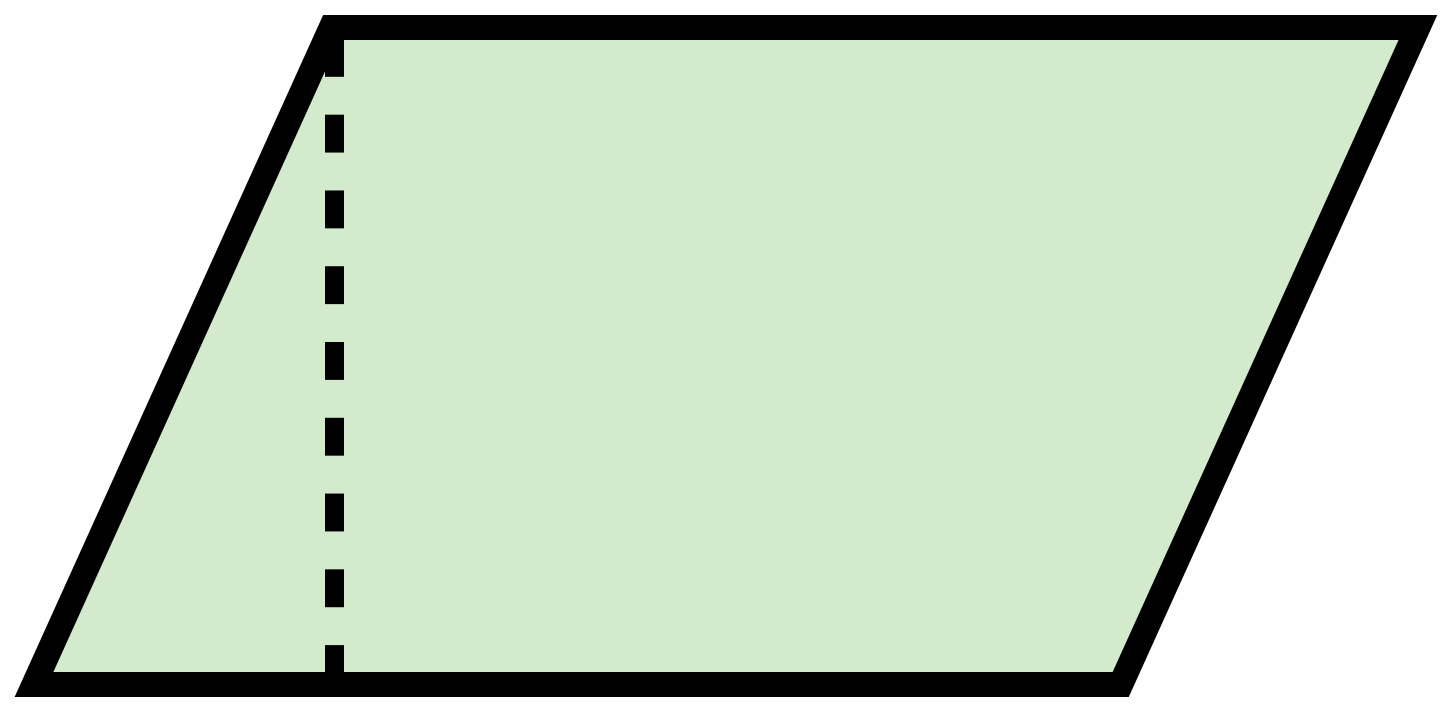
\includegraphics[width=0.25\linewidth]{pictures/5-abb-Vereinigung} 

}

\caption{Repräsentation des Vereinigungsaspektes}\label{fig:FlaecheVereinigung}
\end{figure}

Möchte man die Größe eines Landes bestimmen, so ist es in der Regel notwendig, dieses in geeignete Flächenstücke zu zerlegen, deren Flächeninhalte einfacher berechnet werden können. Dies ist also eine mögliche Anwendung in der Realität. Je nach Komplexität der Figur (und ggf. zusätzlichen geometrischen Überlegungen) können so auch Flächeninhaltsformeln gefunden werden (was schon eine innermathematische Anwendung ist).

\hypertarget{kongruenzaspekt}{%
\subsubsection{Kongruenzaspekt}\label{kongruenzaspekt}}

Wer hat größere Hände? Um diese Frage zu beantworten, ist eine typische Erfahrung, die Hände aneinanderzulegen und ihre Größen zu vergleichen. Dabei wird die Vorstellung genutzt, dass zueinander kongruente Figuren den gleichen Flächeninhalt haben.

Eine Repräsentation, die dabei unterstützt, im Kongruenzaspekt zu operieren, kann in der Teilung oder \emph{Ummantelung} von Figuren mittels zueinander kongruenter Figuren liegen (siehe Abbildung \ref{fig:FlaecheKongruenz}). Dies ist z.~B. bei der Herleitung der Flächeninhaltsformel für ein Dreieck sinnvoll, um zu erkennen, dass dieser der Hälfte des Flächeninhalts des umschriebenen Rechtecks entspricht\footnote{Um diesen Zusammenhang vollumfänglich zu verstehen, sind weiterhin der Vereinigungsapekt (Aufteilen in Teildreiecke) und der Maßzahlaspekt (um die Flächeninhaltsformel fürs Rechteck zu verstehen) nötig.}.

\begin{figure}

{\centering 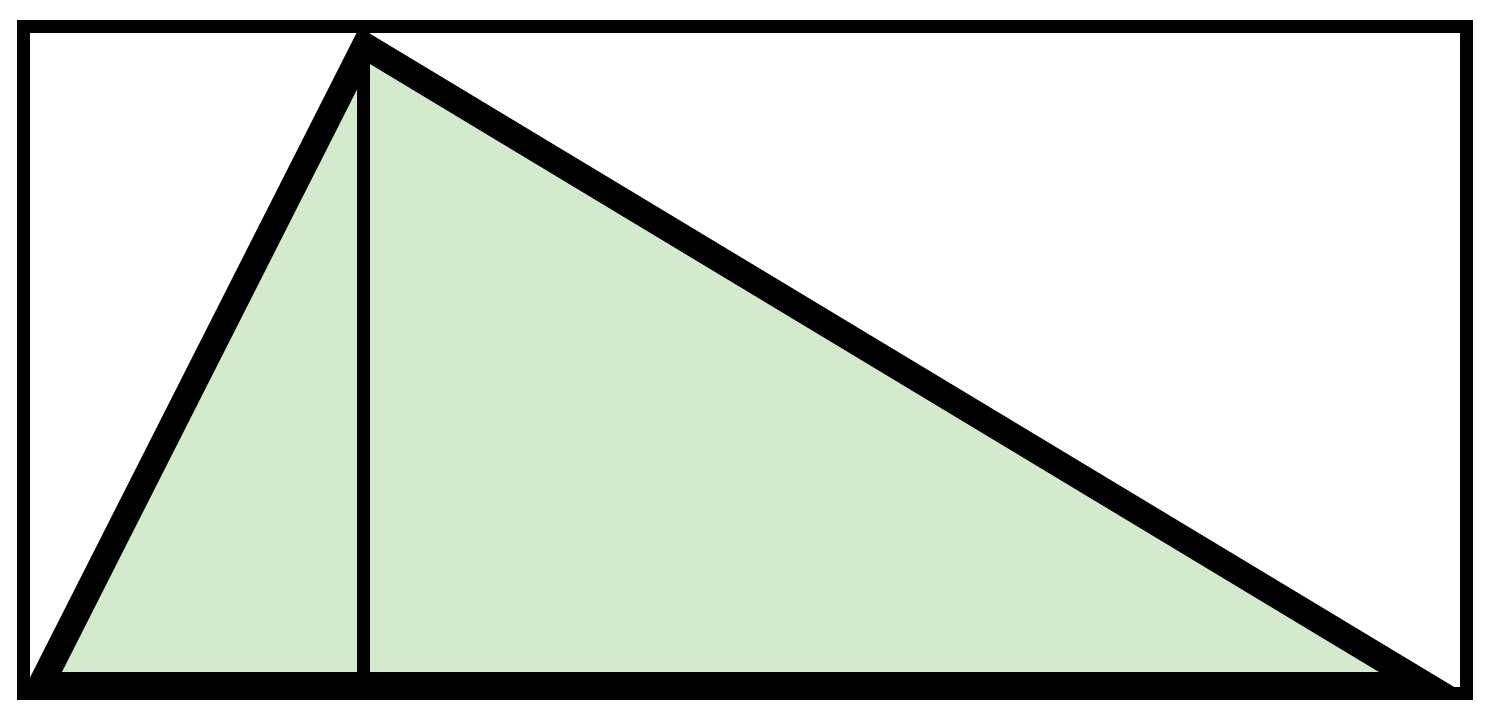
\includegraphics[width=0.25\linewidth]{pictures/5-Kongruenz} 

}

\caption{Repräsentation des Kongruenzaspektes}\label{fig:FlaecheKongruenz}
\end{figure}

Eine (innermathematische) Anwendung dieser Vorstellung könnte zum Beispiel bei der Berechnung des Oberflächeninhalts eines Primas liegen, wo die Flächeninhalte von Grund- und Deckfläche i.~d.~R. nicht einzeln berechnet werden, sondern einer der Flächeninhalte wegen der Kongruenz einfach verdoppelt wird.

\hypertarget{operieren-mit-fluxe4cheninhalten}{%
\subsubsection{Operieren mit Flächeninhalten}\label{operieren-mit-fluxe4cheninhalten}}

Für unterschiedliche Operationen, die mit Flächeninhalten durchgeführt werden, können nun in unterschiedlicher Weise die Grundvorstellungen zu den Aspekten aufgegriffen und genutzt werden:

\begin{itemize}
\tightlist
\item
  Um Flächeninhalte direkt miteinander zu \textbf{vergleichen}, sind der Vereinigungs- und Kongruenzaspekt relevant, da die Flächen ggf. neu aufgeteilt werden müssen und dann mittels Übereinanderlegen gegeneinander abgeschätzt werden können.
\item
  Um die \textbf{Flächeninhaltsformel eines Rechtecks} zu begründen, benötigt es den Maßzahlaspekt, da das Abzählen einbeschriebener Vergleichsquadrate wesentlich ist. Dies hängt auch eng mit der Grundvorstellung der Multiplikation als Rechteckflächeninhalt zusammen (siehe Abbildung \ref{fig:Bruchmultiplikation}).
\item
  Für die \textbf{Flächeninhaltsformel des Dreiecks} sind wieder Kongruenz- und Vereinigungsaspekt relevant, da das Dreieck geeignet zerlegt und mit dem umschriebenen Rechteck verglichen werden muss (siehe Abbildung \ref{fig:FlaecheKongruenz}). Da Bezug zur Rechteckformel genommen wird, ist natürlich auch der Maßzahlaspekt relevant.
\item
  Um \textbf{Flächeninhalte zu approximieren}, wie z.~B. den eines Kreises (siehe Abbildung \ref{fig:FlaecheKreis}), benötigt es wieder alle drei Vorstellungen. So kann der Kreis in zueinander kongruente Teilflächen zerlegt werden (Kongruenz- und Vereinigungsaspekt), deren Gesamtflächeninhalt dann über die Rechteckformel näherungsweise bestimmt wird (Maßzahlaspekt).
\end{itemize}

\begin{figure}

{\centering 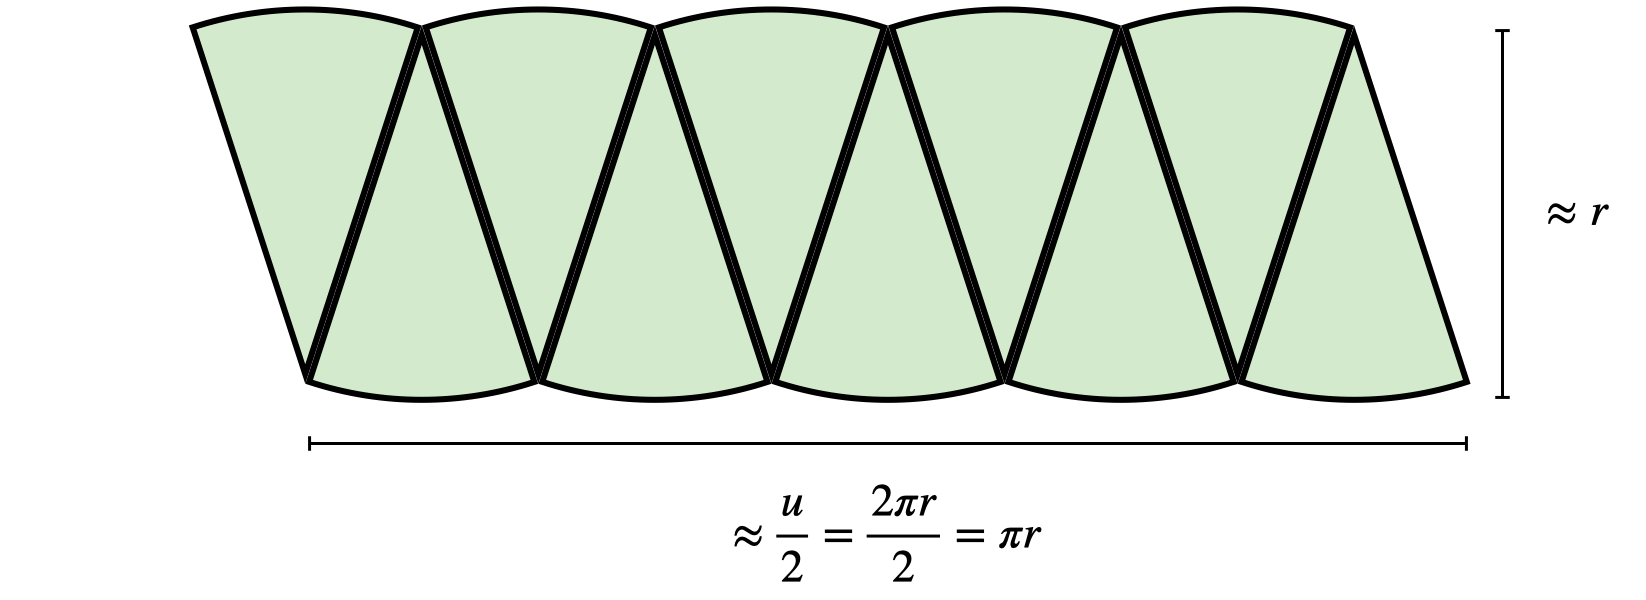
\includegraphics[width=0.75\linewidth]{pictures/5-abb-Kreis} 

}

\caption{Approximation des Kreisflächeninhalts}\label{fig:FlaecheKreis}
\end{figure}

\begin{itemize}
\tightlist
\item
  Bei der \textbf{Bestimmung von Oberflächeninhalten} von Körpern, werden der Vereinigungsaspekt für die einzelnen Seitenflächen und ggf. der Kongruenzaspekt angesprochen, wenn es zueinander kongruente Seitenflächen gibt (wie z.~B. bei Prismen), deren Flächeninhalte dann mit der entsprechenden Anzahl multipliziert und nicht einzeln ausgerechnet werden.
\end{itemize}

\hypertarget{auswirkungen-auf-lernpfad}{%
\subsection{Auswirkungen auf Lernpfad}\label{auswirkungen-auf-lernpfad}}

Der Lernpfad des Schulbuches greift diese Fundamentale Idee und die Grundvorstellungen auf, indem zunächst Flächeninhalte (durch Ausseinanderschneiden und Zusammenfügen) miteinander verglichen werden, anschließend das Auslegen mit normierten Flächenstücken erfolgt und daraufhin geeignete Maßeinheiten eingeführt werden und die Flächeninhaltsberechnung eines Rechtecks behandelt wird.

Die formale und empirische Ebenen wurden hier getrennt dargestellt, was jedoch für eine stoffdidaktische Analyse gar nicht zwingend nötig ist. Entscheidend ist, dass Sie den ganzheitlichen Blick auf die aufgeworfenen Fragen haben und diese (zumindest in Teilen) beantworten können. Die getrennte Darstellung dient hier noch der Übersicht für Sie als \emph{Anfängerinnen und Anfänger} im Umgang mit stoffdidaktischen Analysen -- auch wenn darauf verzichtet wurde, die einzelnen Fragen schrittweise explizit zu beantworten.

\hypertarget{konkrete-ebene-1}{%
\section{Konkrete Ebene}\label{konkrete-ebene-1}}

\begin{quote}
Welche Kernfragen und Kernideen können die Entwicklung der Begriffe, Sätze und Verfahren leiten?
Welche Kontexte und Probleme sind geeignet, um an ihnen die Kernfragen und -ideen exemplarisch zu behandeln und die Inhalte zu rekonstruieren?
Wie kann das Verständnis sukzessive über konkrete Situationen in den beabsichtigten Lernpfaden konstruiert werden (horizontale Mathematisierung)?
Wie können die Lernpfade in Bezug auf die Problemstruktur angeordnet werden (vertikale Mathematisierung)?
\end{quote}

Als \textbf{Kontext} wählt das Schulbuch den Platzbedarf bei \textbf{Tiergehegen im Zoo.} Dieser Kontext ist aus mehreren Gründen besonders gut geeignet:

\begin{itemize}
\tightlist
\item
  In der Regel interessiert tatsächlich nur der Flächeninhalt des Geheges. Inhaltliche Verwechslungen mit dem Umfang oder dem Volumen können damit reduziert werden.
\item
  Es ist aus dem Kontext heraus sinnstiftend, die Größe der Gehege miteinander zu vergleichen, da verschiedene Tiere einen unterschiedlichen Platzbedarf haben.\footnote{Verwiesen wird auch auf ein \emph{Gutachten über Mindestanforderungen an die Haltung von Säugetieren} vom Bundesministerium für Ernährung und Landwirtschaft (\protect\hyperlink{ref-BundesministeriumfurErnahrungundLandwirtschaft2014}{2014}).}
\item
  Verschiedene Formen der Tiergehege lassen sich nutzen, um verschiedene Vergleichsstrategien zu motivieren. So können z.~B. Flächen zerlegt und neu zusammengesetzt werden, runde Formen angenähert werden und durch das Ausschneiden der Figuren ist ein Übereinanderlegen möglich.
\end{itemize}

Dabei werden zwei \textbf{Kernideen} aufgegriffen (\protect\hyperlink{ref-Barzel2012a}{Barzel et al., 2012a, S. 359~f.}):

\begin{itemize}
\tightlist
\item
  Eine besteht im \textbf{Vergleich der Flächeninhalte} der verschiedenen Gehege. Dieses aus dem Kontext heraus begründbare Vorgehen führt im mathematischen Sinne zum Bedürfnis, Flächen zu vermessen, um sie miteiander vergleichen zu können. Als subjektive Kernfrage wird formuliert: »Wie kann ich die Größe von Flächen vergleichen?« (\protect\hyperlink{ref-Barzel2012}{Barzel et al., 2012c, S. 170})
\item
  Die zweite Kernidee ist das \textbf{geschickte Bestimmen eines Flächeninhalts}, wofür zunächst mittels Kästchenpapier das Auszählen von Flächen mit unterschiedlicher Genauigkeit diskutiert wird, anschließend geeignete Maßeinheiten eingeführt werden und die Flächeninhaltsformel des Rechtsecks behandelt wird. Die Formulierung der zugehörigen Kernfrage lautet: »Wie kann ich die Größe von Flächen geschickt bestimmen?« (\protect\hyperlink{ref-Barzel2012}{Barzel et al., 2012c, S. 171})
\end{itemize}

Diese Ideen werden jeweils über die Prozesse des Erkunden, Ordnens und Vertiefens realisiert. Durch dieses Vorgehen\footnote{Prediger et al. (\protect\hyperlink{ref-Prediger2014}{2014}) bezeichnen diese Prozesse auch als \emph{Kernprozesse} des Unterrichtens.} wird das Verständnis sukzessive aufgebaut. Im Erkundungsprozess dient die Kernidee der Vorschauperspektive, während sie beim Ordnen und Vertiefen eher eine rückschauende Perspektive hat. Diese \emph{Objektivierung} wird auch dahingehend sichtbar, dass die Kernfragen im Ordnen-Kapitel nun nicht mehr aus der Ich-Perspektive formuliert werden: »Wie kann man die Größe von Flächen vergleichen?«, »Wie kann man die Größe von Flächen bestimmen?« (\protect\hyperlink{ref-Barzel2012}{Barzel et al., 2012c, S. 176~f.})

\hypertarget{ausblick-auf-empirische-ebene}{%
\section{Ausblick auf empirische Ebene}\label{ausblick-auf-empirische-ebene}}

\begin{quote}
Welche typischen individuellen Voraussetzungen (Vorstellungen, Kenntnisse, Kompetenzen, \ldots) sind zu erwarten und wie passen diese zum angestrebten Verständnis (Ressourcen vs.~Hindernisse)?
Woher kommen typische Hindernisse oder unerwünschte Vorstellungen?
Wie können typische Vorkenntnisse und Vorstellungen als fruchtbare Anknüpfungspunkte dienen?
Welche Schlüsselstellen (Hindernisse, Wendepunkte, \ldots) gibt es im Lernweg der Schülerinnen und Schüler?
Wie kann der angestrebte Lernpfad bezüglich der Anknüpfungspunkte und Schlüsselstellen neu angeordnet werden?
\end{quote}

Kuntze (\protect\hyperlink{ref-Kuntze2018}{2018, S. 159~f.}) verweist auf typische Schwierigkeiten von Schülerinnen und Schülern im Umgang mit dem Flächeninhaltsbegriff.

So kommt es häufig zu einer Verwechslung zwischen Längenmaßen, Flächeninahlten und Volumina. Eine Ursache wird v.~a. in der frühzeitigen kalkülhaften Herangehensweise gesehen, Flächeninhalte über Formeln berechnen zu müssen. So fehlt ein tiefergehendes Begriffsverständnis und die Formeln können nicht sinnstiftend genutzt werden. Dem kann u.~a. dadurch begegnet werden, indem bewusst die Zusammenhänge hergestellt werden, z.~B. zwischen Umfang und Flächeninhalt.
Letztlich zeigen empirische Erhebungen, dass Kinder mit einem vertieften Verständnis über Flächeninhalte auch besser in der Lage sind, entsprechende Formeln anzuwenden (\protect\hyperlink{ref-Worner2014}{Wörner, 2014, S. 1330}).

Weiterhin besteht wegen der Wortverwandtschaft von \emph{Fläche} und \emph{Flächeninhalt} die Gefahr, dass entsprechende Vorstellungen nicht aufgebaut werden, insbesondere dann, wenn die Begriffe (zumindest von der Lehrkraft) nicht sauber getrennt verwendet werden. Die Fläche ist die Figur an sich und wird über ihre \emph{Form} bestimmt. Der Flächeninhalt ist ein \emph{Maß} für die Größe der Figur (vgl. \protect\hyperlink{ref-Barzel2012a}{Barzel et al., 2012a, S. 362}). Insbesondere für Schülerinnen und Schüler, deren Muttersprache nicht Deutsch ist, kann die fehlerhafte Verwendung dieser feinen Unterschiede hinderlich dabei sein, dem Unterricht zu folgen.

Derartige Schwierigkeiten werden im Schulbuch implizit aufgegriffen (z.~B. strikte sprachliche Trennung) oder explizit thematisiert (z.~B. verbindende und vergleichende Behandlung mit dem Umfang von Figuren), so dass auch dies wieder die Gestaltung des Lernpfades beeinflusst.

\hypertarget{erstesintermezzo-nachbereitung}{%
\section{Zum Nachbereiten}\label{erstesintermezzo-nachbereitung}}

\begin{enumerate}
\def\labelenumi{\arabic{enumi}.}
\tightlist
\item
  Diskutieren Sie zu weiteren typischen Operationen mit Flächeninhalten, welche Grundvorstellungen dafür aufgegriffen und genutzt werden.
\item
  Finden Sie einen alternativen Kontext (statt den Zoogehegen), der geeignet ist, die Kernideen so aspektreich durchzuarbeiten.
\end{enumerate}

\hypertarget{part-lernprozesse-gestalten}{%
\part*{Lernprozesse gestalten}\label{part-lernprozesse-gestalten}}
\addcontentsline{toc}{part}{Lernprozesse gestalten}

\hypertarget{lerntaetigkeit-und-lernhandlungen}{%
\chapter{Lerntätigkeit und Lernhandlungen}\label{lerntaetigkeit-und-lernhandlungen}}

\begin{quote}
\textbf{Ziele}

\begin{itemize}
\tightlist
\item
  Sie kennen Grundideen der Tätigkeitstheorie, insbesondere bezüglich Lehr-Lern-Prozesse.
\item
  Sie können geeignete Lernhandlungen für Lerngegenstände formulieren.
\item
  Sie kennen Möglichkeiten, wie Lernhandlungen in verschiedenen Unterrichtsphasen ausgebildet werden können.
\end{itemize}

\textbf{Material}

\begin{itemize}
\tightlist
\item
  Folien zur Vorlesung zu Lerntätigkeit und Lernhandlungen (\href{files/Stoffdidaktik-WiSe2223-Kap6.pdf}{pdf}, \href{files/Stoffdidaktik-WiSe2223-Kap6.key}{Keynote})
\end{itemize}
\end{quote}

Mit den Kapiteln \ref{fundamentale-ideen} bis \ref{erstes-intermezzo-flaecheninhalt} haben Sie Ansätze kennengelernt, die Fragen der \textcolor{formalColor}{formalen}, \textcolor{semanticColor}{semantischen} und \textcolor{concreteColor}{konkreten} Ebene des \protect\hyperlink{tab:fragen-ebenen}{Vier-Ebenen-Ansatzes} nach Hußmann \& Prediger (\protect\hyperlink{ref-Hussmann:2016}{2016}) zu beantworten. Mit der deskriptiven Perspektive auf Grundvorstellungen kennen Sie auch schon erste Grundlagen, Fragen der \textcolor{empiricColor}{empirischen} Ebene zu untersuchen. Ziel bei all den Fragen war immer, \textbf{Lernpfade} für Lerngegenstände zu generieren, also den Stoff derart auszuwählen (\emph{spezifizieren}) und anzuordnen (\emph{strukturieren}), dass er sinnstiftend gelehrt und gelernt werden kann.

Nach einer solchen stoffdidaktischen Analyse ist nun der nächste Schritt die Planung der Unterrichtsgestaltung an sich. In der fachdidaktischen und bildungswissenschaftlichen Literatur hat sich hierfür der Begriff der \textbf{Lernumgebung} durchgesetzt -- dabei aber auch mit verschiedenen Sichtweisen wie eine »pädagogische« (z.~B. angenehme Lernatmosphäre, respektvolles Miteinander), als ein »methodisch-organisatorisches Arrangement« (z.~B. Gestaltung des Klassenraums) oder eben auch als »inhaltliches Verständnis«, das hier weiter verfolgt werden soll (vgl. \protect\hyperlink{ref-Krauthausen:2018}{Krauthausen, 2018, S. 255}).

Nach Leuders (\protect\hyperlink{ref-Leuders2015}{2015, S. 448}) beinhalten Lernumgebungen für den Mathematikunterricht \textbf{»i) ein nach bestimmten Prinzipien geordnetes System von Aufgaben, ii) methodische Organisationsformen und iii) Stützsysteme, wie z.~B. Medien, Lehrerinterventionen und Kommunikationsformen«}. Die Grundlagen für die entsprechenden Bestandteile lernten und lernen Sie v.~a. in den weiteren Veranstaltungen der Fachdidaktiken und Bildungswissenschaften sowie in Ihrer schulpraktischen Ausbildung (und auch noch während Ihrer Tätigkeit als voll ausgebildete Lehrkraft). Bezogen auf stoffdidaktische Überlegungen dienen die folgenden drei Kapitel dabei noch einmal einer Schwerpunktbildung:

\begin{itemize}
\item
  In diesem Kapitel werden zunächst allgemein Erkenntnisse über \emph{Lehr-Lern-Prozesse} diskutiert. Dabei wird auf \textbf{tätigkeitstheoretische Grundlagen} Bezug genommen. Diese theoretische Grundlage ist dabei \emph{eine} von vielen Möglichkeiten, Lehren und Lernen zu beschreiben und zu erklären, und wird hier aufgrund ihrer Betonung stofflicher Inhalte sowie als Forschungsschwerpunkt und in der Tradition der Potsdamer Mathematiklehrkräftebildung verwendet (siehe z.~B. \protect\hyperlink{ref-Etzold2021}{Etzold, 2021, S. 13}). Sie sollten natürlich offen und neugierig genug sein, sich auch anderen Theorien zu widmen und diese für Ihre Unterrichtsplanung heranzuziehen.
\item
  Von den \emph{Medien} (zu denen ja beispielsweise auch die Tafel, Computer oder Zettel und Stift gehören -- der entsprechende Medienbegriff sollte Ihnen aus den Bildungswissenschaften bekannt sein) werden im nächsten Kapitel v.~a. \textbf{Arbeitsmittel}\footnote{In der englischsprachigen Literatur werden \emph{Arbeitsmittel} oft als \emph{manipulatives} bezeichnet. Dies soll nicht ausdrücken, dass diese Arbeitsmittel in irgendeiner Weise manipulierend auf die Schülerin oder den Schüler wirken, sondern dass die Schülerinnen und Schüler selbst das Arbeitsmittel verändern bzw. mit dessen Hilfe auf den Lerngegenstand einwirken (siehe auch \protect\hyperlink{ref-enwiki:1023437370}{Wikipedia contributors, 2021}).} herausgegriffen. Diese »repräsentieren mathematische Objekte und erlauben zudem Handlungen oder Operationen mit diesen Objekten« (\protect\hyperlink{ref-Schmidt-Thieme2015}{Schmidt-Thieme \& Weigand, 2015, S. 461~f.}) Im Sinne der Tätigkeitstheorie dienen sie damit als Mittler zwischen Lerngegenstand und Schülerin bzw. Schüler. Im Schulalltag wird es in der Regel Ihre Aufgabe sein, derartige Arbeitsmittel zu \textbf{analysieren}, um sie zielgerichtet auszuwählen und im Unterricht einzusetzen.
\item
  Eng verbunden mit dem Einsatz von Arbeitsmitteln sind \textbf{Aufgaben}, die Sie den Schülerinnen und Schülern stellen. Aufgaben können dabei »als Aufforderung an Lernende zum mathematischen Handeln aufgefasst« werden (\protect\hyperlink{ref-Leuders2015}{Leuders, 2015, S. 435}). Neben der Auswahl von Aufgaben werden Sie als Lehrkraft aber insbesondere Aufgaben \textbf{gestalten}, also selbst welche entwickeln und vorhandene Aufgaben variieren und an Ihre Lerngruppe anpassen. Maßnahmen hierzu finden sich im übernächsten Kapitel.
\end{itemize}

\hypertarget{taetigkeitstheorie-und-lernen}{%
\section{Tätigkeitstheorie und Lernen}\label{taetigkeitstheorie-und-lernen}}

Eine Grundannahme der Tätigkeitstheorie, die auf Vygotskijs psychologische Arbeiten aus den 1920er Jahren in der Sowjetunion zurück geht, ist das Verständnis, dass sich \textbf{Individuen aktiv-handelnd mit ihrer Umwelt auseinandersetzen}, \textbf{die Umwelt} dabei in der Interaktion mit der Gesellschaft \textbf{verändern}, und beide Prozesse wiederum psychisch im Individuum abgebildet werden. Dies widerspricht bspw. der \emph{behavioristischen} Annahme, dass man sich seiner Umwelt einfach nur anpasst, aber es ist auch nicht mit einer streng \emph{konstruktivistischen} Annahme zu verwechseln, nach der Individuen ein Abbild der Umwelt kognitiv rekonstruieren. Die Tätigkeitstheorie kann eher als »(moderat) konstruktivistische{[}r{]}{[}..{]} Ansatz« bezeichnet werden (\protect\hyperlink{ref-Giest2016a}{Giest, 2016, S. 47}).

Zu betonen ist dabei die \textbf{beiderseitige Wirkrichtung}: Sowohl das Individuum wirkt auf die Umwelt ein (und verändert sie, es kommt zur \emph{gesellschaftlichen Weiterentwicklung}), als auch die Umwelt auf das Individuum (was zur \emph{Persönlichkeitsentwicklung} führt). Beide Prozesse sind dabei nicht voneinander zu trennen. Eine solche Interaktion ist von (gesellschaftlich entwickelten) Motiven geprägt und wird als \textbf{\emph{Tätigkeit}} bezeichnet. Giest \& Lompscher (\protect\hyperlink{ref-Giest2006}{2006, S. 27}) formulieren: »Er {[}der Mensch{]} erschafft damit seine Kultur und zugleich die psychischen Funktionen, die ihn dazu in die Lage versetzen.« Dieses Paradoxon, dass die Tätigkeit ihre eigene Voraussetzung ist, kann aufgelöst werden, indem man zunächst kultur-historisch die gemeinschaftliche und erst dann die individuelle Tätigkeit betrachtet: »Durch (gemeinsame) Tätigkeit erfolgte die (kulturelle) Meschwerdung und über ihre individuelle Aneignung verläuft die Persönlichkeitsentwicklung« (\protect\hyperlink{ref-Giest2006}{Giest \& Lompscher, 2006, S. 27}).

Für schulische Prozesse von besonderem Interesse ist die \textbf{\emph{Lerntätigkeit}}, in der Definition nach Giest \& Lompscher (\protect\hyperlink{ref-Giest2006}{2006, S. 67}):

\begin{definition}[Lerntätigkeit]
\protect\hypertarget{def:Lerntaetigkeit}{}\label{def:Lerntaetigkeit}Lerntätigkeit kann man definieren als die speziell auf die Aneignung gesellschaftlichen Wissens und Könnens (Lerngegenstände) gerichtete Tätigkeit, wozu spezifische Mittel (Lernmittel) unter speziell gestalteten Bedingungen eingesetzt werden müssen.
\end{definition}

Giest \& Lompscher (\protect\hyperlink{ref-Giest2006}{2006, S. 67}) führen fort: »Da die Lerngegenstände und Lernmittel kultureller Natur sind, kann Lerntätigkeit auch nur im Rahmen der Kultur, der Kooperation und Kommunikation mit denen, die über diese Kultur verfügen, angeeignet werden.« Dies betont in der Unterrichtsrealität u.~a. die besondere Bedeutung und Verantwortung der Lehrkraft als wissende Person, die den Lernprozess der Schülerinnen und Schüler steuert. Dies heißt nicht, dass Unterricht lehrerzentriert gestaltet werden soll, ganz im Gegenteil: Entscheidend ist, dass die Lehrperson die Schülerinnen und Schüler dazu befähigt, sich den Lerngegenstand anzueignen, etwa indem sie geeignete Lernmittel zur Verfügung stellt und den Umgang mit ihnen schult.

Auch unabhänging vom Lernen sind Tätigkeiten stets auf einen \textbf{Gegenstand} bezogen, können also niemals inhaltsleer erfolgen. Tätigkeiten basieren dabei auf \textbf{Motiven}, d.~h. »innere Antriebe« (\protect\hyperlink{ref-Giest2006}{Giest \& Lompscher, 2006, S. 39}). Im Kontext des Lernens sind dies insbesondere die Motive \emph{Interesse}, \emph{Leistung}, \emph{Affiliation} (soziale Nähe) und \emph{Neugierde} (\protect\hyperlink{ref-Mienert2011}{Mienert \& Pitcher, 2011, S. 57}). In der Konfrontation mit einem Gegenstand bildet das Individuum, basierend auf die Motive, \textbf{Ziele} als »ideell vorweggenommene Resultate der Tätigkeit« aus (\protect\hyperlink{ref-Giest2006}{Giest \& Lompscher, 2006, S. 39}), was zu \textbf{Handlungen} im Zusammenhang mit dem Gegenstand führt. Handlungen dienen also der (zielgerichteten) Realisierung der Tätigkeit.
Im Rahmen der \emph{Lerntätigkeit} führt dies dann zu \textbf{\emph{Lernhandlungen}}. Lompscher (\protect\hyperlink{ref-Lompscher1983}{1983b, S. 46}) definiert:

\begin{definition}[Lernhandlung]
\protect\hypertarget{def:Lernhandlung}{}\label{def:Lernhandlung}Lernhandlungen sind relativ geschlossene und abgrenzbare, zeitlich und logisch strukturierte Abschnitte im Verlauf der Lerntätigkeit, die ein konkretes Lernziel realisieren, durch bestimmte Lernmotive angetrieben werden und entsprechend den konkreten Lernbedingungen durch den Einsatz äußerer und verinnerlichter Lernmittel in einer jeweils spezifischen Folge von Teilhandlungen vollzogen werden.
\end{definition}

\hypertarget{typische-lernhandlungen}{%
\section{Typische Lernhandlungen}\label{typische-lernhandlungen}}

Unabhängig von konkreten Lerngegenständen haben Bruder \& Brückner (\protect\hyperlink{ref-Bruder1989}{1989}) typische Lernhandlungen für den Mathematikunterricht strukturiert beschrieben (Hervorhebungen im Original, auch dargestellt bei \protect\hyperlink{ref-Feldt-Caesar2017}{Feldt-Caesar, 2017, S. 87~ff.}):

\hypertarget{elementare-aneignungshandlungen}{%
\subsection{Elementare Aneignungshandlungen}\label{elementare-aneignungshandlungen}}

\begin{itemize}
\tightlist
\item
  \textbf{Identifizieren:} »Vergleichen der aufgenommenen Informationen zu Teilen oder Eigenschaften eines Objektes mit den Merkmalen bestimmter aktualisierter Abbilder (Stoffelemente, Handlungsvorschriften \ldots) und Feststellung von Übereinstimmung oder Nichtübereinstimmung auf der Grundlage eines den jeweiligen Abbildungsmerkmalen entsprechenden \emph{Idealisierens} der gegebenen Objektsituation«
\item
  \textbf{Realisieren:} »\emph{Transferieren}, Konkretisieren oder Spezialisieren eines vorgegebenen (bzw. identifizierten) Handlungsgegenstandes (Stoffelemente, Vorgehensstrategien \ldots) auf eine gegebene Objektsituation und \emph{Zusammenfügen} der so erzeugten Teile zu einem neuen Ganzen«
\end{itemize}

\hypertarget{grundhandlungen}{%
\subsection{Grundhandlungen}\label{grundhandlungen}}

\begin{itemize}
\tightlist
\item
  \textbf{Erkennen:} »Ausgliedern wahrgenommener Informationen aus der Aufgabenstellung und Inbeziehungsetzen mit ausgegliederten bekannten (gespeicherten) Abbildern bzw. der neu zusammengefügten Abbilder, bis eine Übereinstimmung festgestellt wird«
\item
  \textbf{Beschreiben:} »Identifizieren und Realisieren einer dem gespeicherten (oder erzeugten) Abbild adäquaten umgangssprachlichen Formulierung oder Darstellung in mathematischer Terminologie und Symbolik und Entäußerung der Informationen auf sprachlicher oder materialisierter Ebene«
\item
  \textbf{Verknüpfen:} »\emph{Transferieren} und \emph{Zusammensetzen} von Zusammenhängen (Sätzen, Verfahren) oder Vorgehensstrategien zu einem neuen Ganzen durch Ersetzungen in der Ausgangskonstellation von Zusammenhängen«
\item
  \textbf{Anwenden:} »Feststellen der Übereinstimmung von den Bedingungen der Aufgabenstellung mit der Ausgangskonstellation der zu realisierenden gegebenen (oder erzeugten) Handlungsvorschrift (Identifizieren) und ggf. Herstellen einer solchen Übereinstimmung (Transferieren)«
\item
  \textbf{Begründen:} »a) Vergleichen eines vorgegebenen Sachverhalts mit gegebenen bzw. bekannten Normativen; b) Realisieren gegebener bzw. identifizierter elementarer Beweisverfahren«
\end{itemize}

\hypertarget{komplexe-handlungen}{%
\subsection{Komplexe Handlungen}\label{komplexe-handlungen}}

\begin{itemize}
\tightlist
\item
  \textbf{Suchen:} »Ergebnis von Suchhandlungen sind zieltaugliche Mittel (Stoffelemente, Zuordnungen, Vorgehensstrategien) zur Lösung der gestellten Aufgabe -- gewonnen durch mehr oder weniger bewußte Anwendung von Suchstrategien«
\item
  \textbf{Planen:} »Durch Anwenden von Vorgehensstrategien wird ein Arbeitsplan mit den erforderlichen Teilschritten zur Zielrealisierung entwickelt«
\item
  \textbf{Ausführen:} »Abarbeiten eines Arbeitsplanes -- Handlungsvollzug auf der Grundalge der ausgebildeten Orientierungsgrundlage u.a. als Berechnen, geometrisches Darstellen, Definieren, Darstellen eines Beweises«
\item
  \textbf{Kontrollieren:} »Feststellen der Zweckmäßigkeit und Exaktheit von Teilschritten des Aufgabenlösens und des Resultats (Handlungsprodukt!)«
\end{itemize}

Diese Handlungen müssen nun je nach Lerngegenstand noch konkretisiert werden. Am Beispiel des Winkelfeldes in Abschnitt \ref{konkrete-ebene} lautete eine Aufgabe für die Schülerinnen und Schüler: »Wo muss das Schaf lang laufen, damit es die gesamte Zeit gerade so von der Kuh gesehen wird?« Hierfür bewegen die Schülerinnen und Schüler in der App das Schaf entlang der Sichtfeldgrenze der Kuh, geradlinig und in Richtung der Augen der Kuh begrenzt und in die andere Richtung unbegrenzt. Sie \emph{identifizieren und realisieren} damit das mathematische Objekt \emph{Strahl}, gebunden am Kontext der Sichtfelder. Im Anschluss wird diese Handlung (kontextunabhängig) verallgemeinert und die Strahl-Eigenschaft des Schenkels charakterisiert. Die App als Lernmittel unterstütz diesen Prozess, indem sich die Bestandteile des Winkelfeldes ein- und ausblenden lassen sowie vom \emph{Tiermodus} in den \emph{Winkelfeldmodus} gewechselt werden kann.



\begin{figure}

{\centering 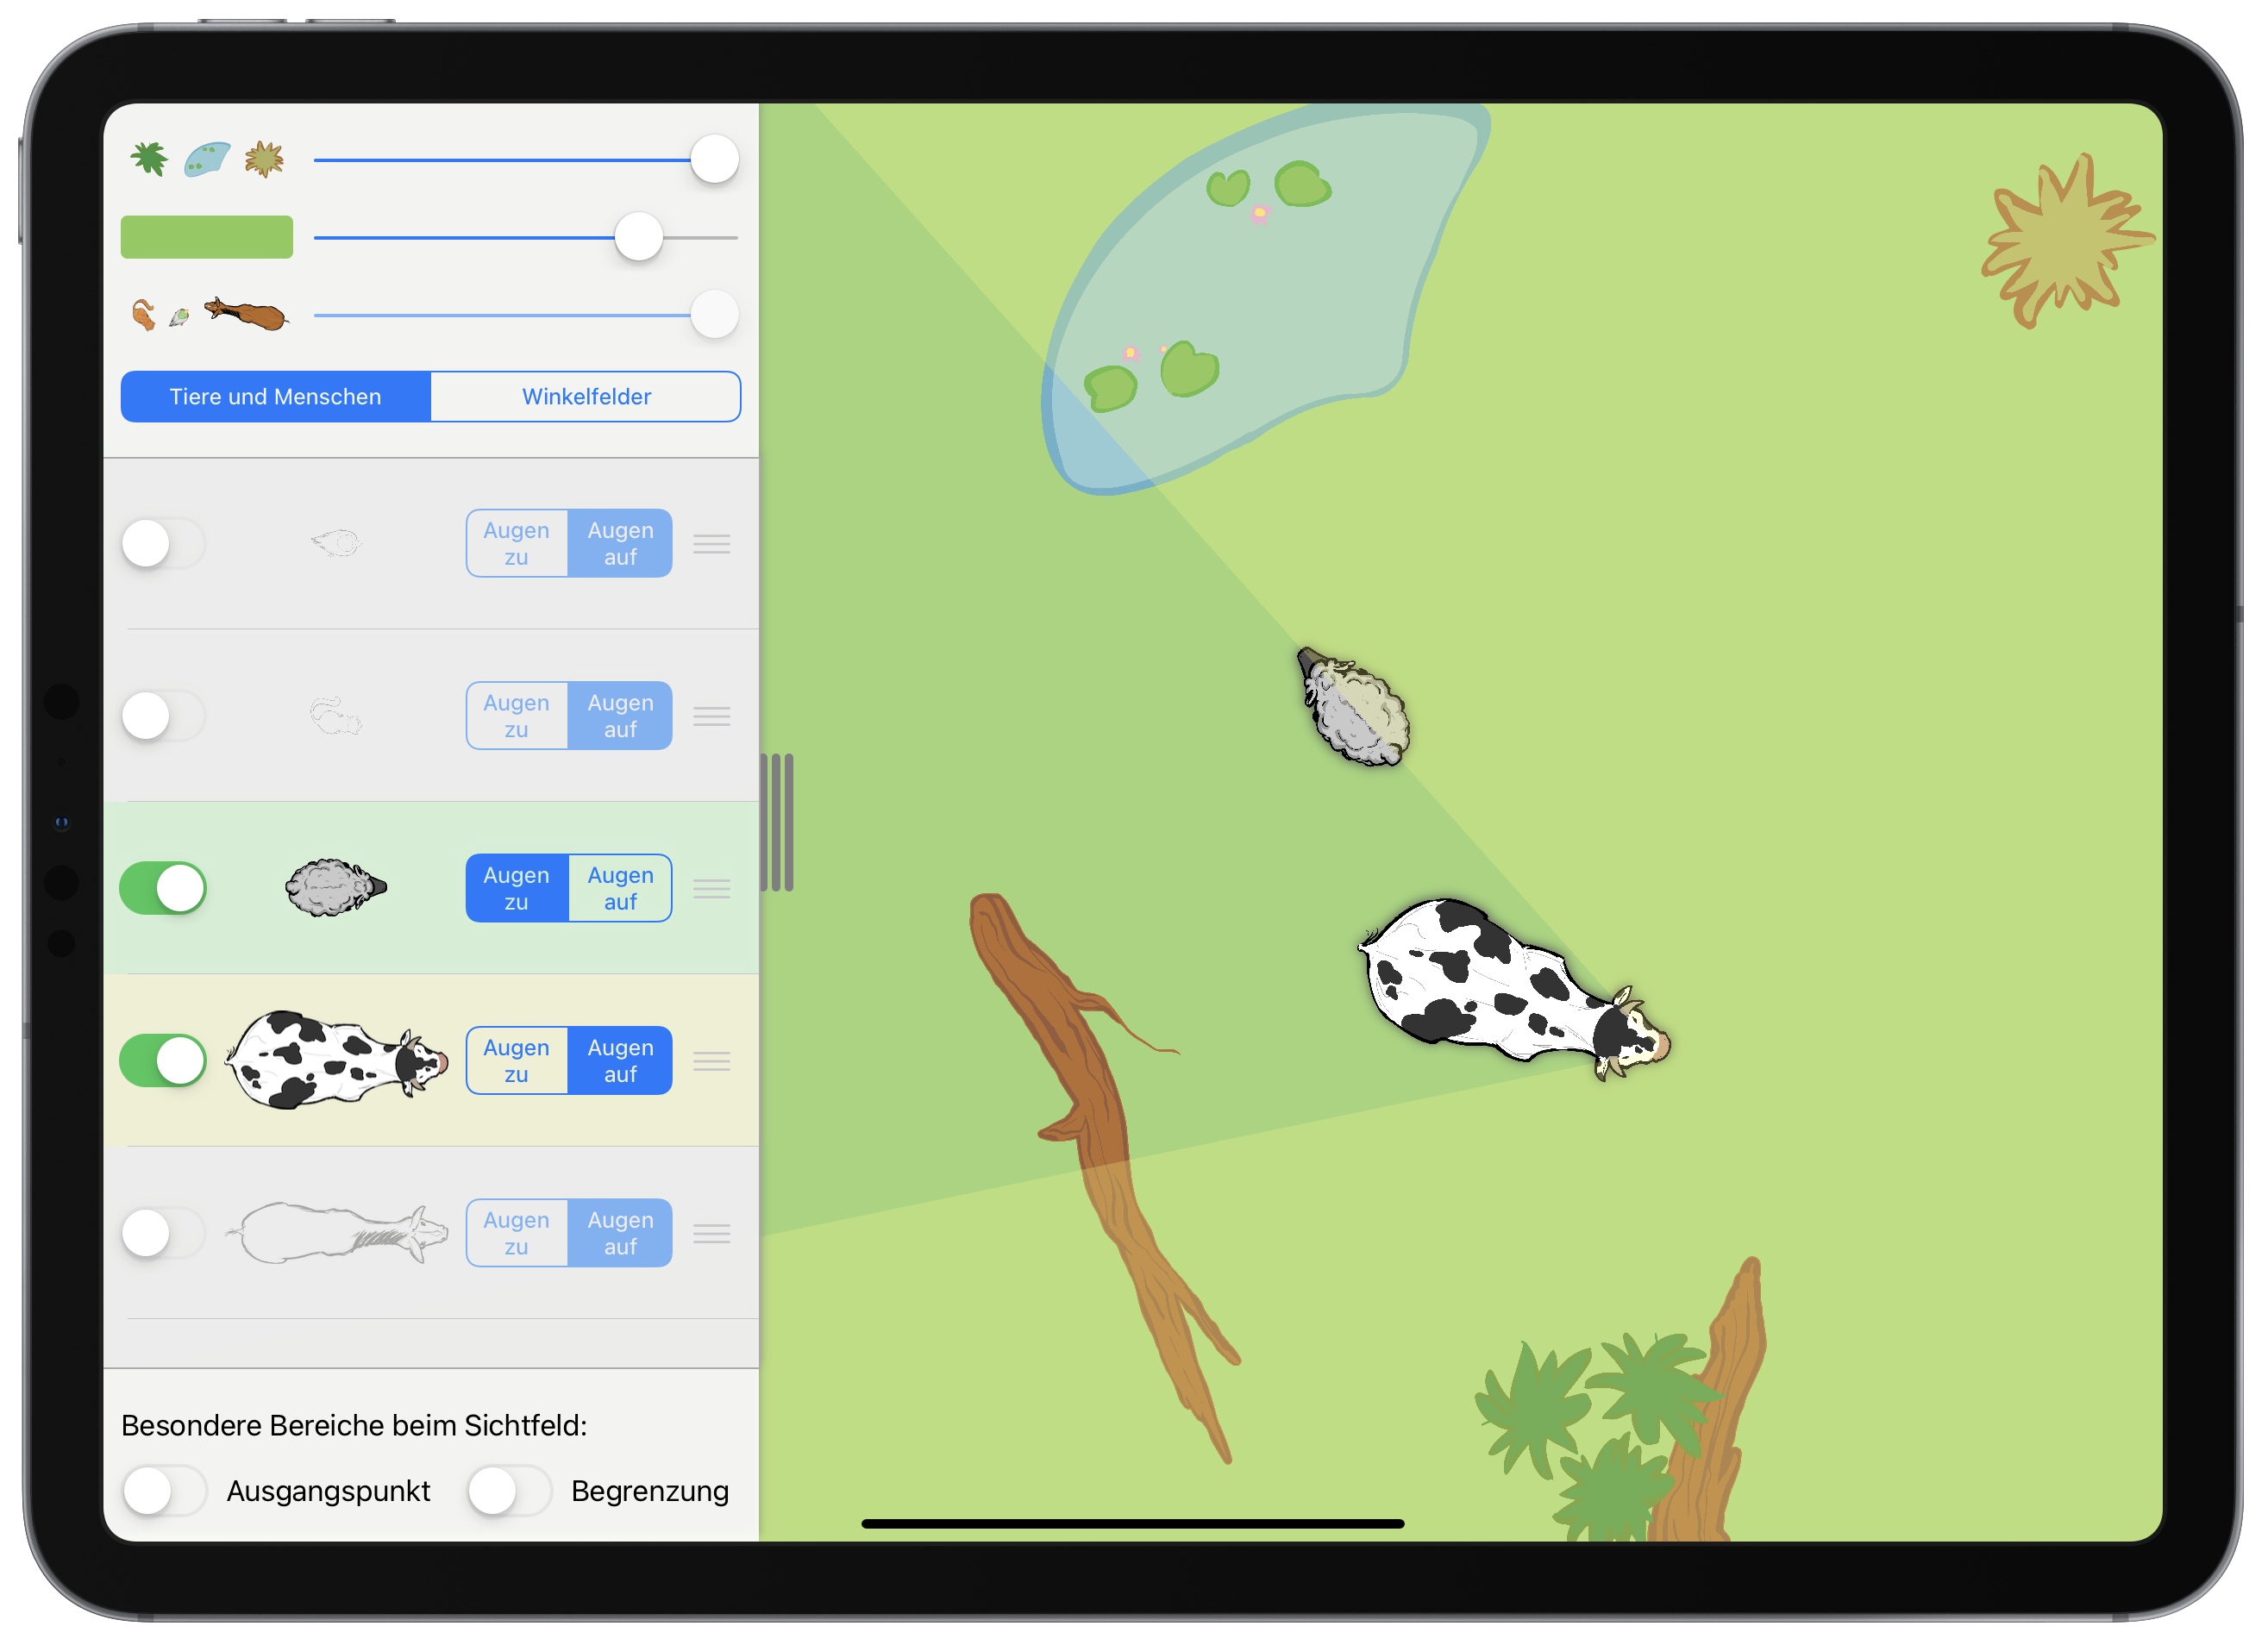
\includegraphics[width=0.5\linewidth]{pictures/1-Winkelfarm} 

}

\caption{Lernhandlung in der App \emph{Winkel-Farm} (\protect\hyperlink{ref-Etzold:2019}{Etzold, 2019a})}\label{fig:HandlungSchaf}
\end{figure}

\hypertarget{lernhandlungen-ausbilden}{%
\section{Lernhandlungen ausbilden}\label{lernhandlungen-ausbilden}}

Lernhandlungen sind zwar notwendig, um sich einem Lerngegenstand zu nähern, müssen selbst jedoch auch erst einmal (am Lerngegenstand) ausgebildet werden. Weiterhin sollen die Lernhandlungen verinnerlicht werden, um sie in Transfersituationen anwenden und komplexere Handlungen darauf aufbauen zu können. Die Qualität der Lernhandlungen verändert sich also im Lernprozess, was sich in verschiedenen Phasen des Unterrichtsgeschehens widerspiegelt.

An dieser Stelle soll auf die von Prediger et al. (\protect\hyperlink{ref-Prediger2013}{2013, S. 770}) fomulierten (und nicht originär auf die Tätigkeitstheorie basierenden\footnote{Prediger et al. (\protect\hyperlink{ref-Prediger2014}{2014, S. 83}) erwähnen hier einen Zusammenhang zu \emph{typischen Unterrichtssituationen}, die Bruder (\protect\hyperlink{ref-Bruder1991}{1991}), basierend auf tätigkeitstheoretischen Grundlagen, formuliert.}) vier \textbf{\emph{Kernprozesse}} einer Unterrichtssequenz zurückgegriffen werden, die auch den Aufbau der \emph{Mathewerkstatt} (\protect\hyperlink{ref-Barzel2012}{Barzel et al., 2012c}) leiten:

\begin{itemize}
\tightlist
\item
  Kernprozess des \textbf{Anknüpfens} an Vorerfahrungen und Interessen
\item
  Kernprozess des \textbf{Erkundens} neuer Zusammenhänge
\item
  Kernprozess des \textbf{Ordnens} als Systematisieren und Sichern
\item
  Kernprozess des \textbf{Vertiefens} durch Üben und Wiederholen.
\end{itemize}

Im Folgenden wird dargestellt, wie einzelne aus der Tätigkeitstheorie stammenden Aspekte zur Ausbildung von Lernhandlungen helfen können, die Kernprozesse, auch unter der stoffdidaktischen Perspektive des Vier-Ebenen-Ansatzes, zu unterstützen. Während die Kernprozesse im Unterricht relativ klar voneinander getrennt werden sollten (weil sie unterschiedliche Funktionen verfolgen), wirken die Theorieelemente teils prozessübergreifend, was sich in den folgenden Überschriften widerspiegelt.

\hypertarget{anknuepfen}{%
\subsection{Anknüpfen}\label{anknuepfen}}

Die Schülerinnen und Schüler müssen zunächst in die Lage versetzt werden, sich mit dem Lerngegenstand auseinandersetzen zu \emph{wollen}. Hierzu ist es hilfreich, die Anforderungssituation in der \textbf{Zone der nächsten Entwicklung} der Schülerinnen und Schüler zu präsentieren. Dabei handelt es sich um eine Problemsituation, Aufgabe oder Fragestellung, die die Schülerinnen und Schüler zwar mithilfe ihrer bisherigen Kenntnisse, Fähigkeiten und Fertigkeiten verstehen und nachvollziehen können, zu ihrer Lösung sie jedoch noch nicht selbstständig in der Lage sind. Somit wird eine Motivation geschaffen, sich mit der Thematik tiefer auseinanderzusetzen. Es ist durchaus möglich, an dieser Stelle auch schon erste Lösungsversuche zu unternehmen. Daran ist besonders gut zu erkennen, »was wir nicht wissen bzw. können, um die Anforderung zu bewältigen« (\protect\hyperlink{ref-Lompscher1996}{Lompscher, 1996, S. 4}).

Anschließend werden gemeinsam mit der Lehrkraft die \textbf{Lernziele} herausgearbeitet, die den weiteren Verlauf des Lernens strukturieren sollen. Wichtig ist hier eine Unterscheidung zu \emph{Lehrzielen}, die die Sicht der Lehrkraft widerspiegeln. \emph{Lernziele} dagegen sind die Ziele aus Sicht der Schülerinnen und Schüler, auf die sich im individuellen Lernprozess auch bezogen werden können muss. Es bietet sich daher auch eine explizite Formulierung der Lernziele an.

In dieser ersten Phase der Ausbildung von Lernhandlungen sollte gemäß Kapitel \ref{kernideen-kernfragen-kontexte} auf einen geeigneten \textbf{Kontext} zurückgegriffen werden, um den Lerngegenstand zu motivieren, und die \textbf{Kernideen bzw. Kernfragen} sollten leitend für die Fomulierung der Lernziele sein.

Sowohl in der Anforderungssituation als auch in der Formulierung der Lernziele zeigt sich erneut die \textbf{Bedeutung der Lehrkaft}: Sie ist diejenige, die die Schülerinnen und Schüler in die Lage versetzen kann, sich dem Lerngegenstand zu nähern. Das heißt insbesondere auch, dass ein \emph{Ostereiersuchen} vermieden werden muss (bei dem die Schülerinnen und Schüler z.~B. so lange raten, um was es denn heute gehen könnte, bis sie die richtige Antwort gefunden haben), sondern die Lehrkraft \emph{instruiert} (persönlich oder durch geeignete Aufgabenstellungen) unter Berücksichtigung der individuellen Voraussetzungen der Schülerinnen und Schüler einen ersten Zugang zum Lerngegenstand. Im Sinne der tätigkeitstheoretischen Grundlagen ist die Lehrkraft damit ein Vertreter des gesellschaftlichen Wissens und Könnens, das sich die Schülerinnen und Schüler als Kenntnisse, Fähigkeiten und Fertigkeiten aneignen werden.

\hypertarget{anknuepfen-erkunden}{%
\subsection{Anknüpfen/Erkunden}\label{anknuepfen-erkunden}}

Mit der Anforderungssituation geht ad hoc eine Orientierung der Schülerinnen und Schüler bezüglich der Einwirkung auf den Lerngegenstand einher. Dies erfolgt noch, bevor überhaupt Lernhandlungen ausgeführt werden (also noch vor dem \emph{Erkunden}), es handelt sich also um eine rein kognitive Dimension. Dabei wird in drei Qualitäten von Orientierungsgrundlagen unterschieden (als Zitate gekennzeichnete Formulierungen sind entnommen aus \protect\hyperlink{ref-Feldt-Caesar2017}{Feldt-Caesar, 2017, S. 83~ff.}):

\begin{itemize}
\item
  \textbf{Probierorientierung:} Die Schülerinnen und Schüler verfügen noch nicht über für die Anforderung nötigen Kenntnisse, Fähigkeiten oder Fertigkeiten. Stattdessen gehen sie nach Versuch und Irrtum vor. Dabei fehlt ihnen »häufig die Einsicht, warum eine bestimmte Handlung zum Erfolg geführt hat, eine andere jedoch nicht. {[}\ldots{]} Aufgrund der mangelnden Einsicht in die wirklichen Bedingungen der Handlungen ist eine erfolgreiche Handlung nicht notwendigerweise reproduzierbar.« Dies führt dazu, dass erfolgreiche Handlungen kaum auf veränderte Situationen übertragen werden können. Eine derartige Orientierung ist also höchstens »in Aneignungsprozessen zu einem Explorieren des neuen Inhaltsbereichs« wünschenswert, darüber hinaus jedoch sollten höhere Orientierungsgrundlagen angestrebt werden.
\item
  \textbf{Musterorientierung:} Die Schülerinnen und Schüler gehen nun nicht mehr nach Versuch und Irrtum vor, sondern orientieren sich an bereits erfolgreich durchgeführten Handlungen in ähnlichen Anforderungssituationen -- die sozusagen als Muster dienen.
  »Dieser Orientierungstyp ist nur dann erfolgreich, wenn die gegebene Anforderungssituation dem erlernten Muster ähnlich genug ist, um eine Passung zu ermöglichen. Tragfähig ist ein Muster nur dann, wenn seine Handlungsbedingungen genau gekannt und stets geprüft werden.«
  Es handelt sich also zwar um eine vollständige Orientierungsgrundlage, jedoch ist eine Transferierbarkeit nicht immer gegeben. Auch kann die »fälschliche Erkennung eines Musters in einer gegebenen Anforderungssituation« zu einer fehlerhaften Übertragung führen.
\item
  \textbf{Feldorientierung:} Die Schülerinnen und Schüler sind nun »nicht an eine konkrete Anforderungssituation gebunden, sondern beziehen sich vielmehr auf ganze Anforderungsklassen. Durch das Erkennen der Passung einer solchen Anforderungsklasse kann sich der Lernende für konkrete Situationen selbst eine Orientierung schaffen. Er verfügt über einen gewissen Überblick über die Situation und ist in der Lage zu differenzieren, welche Stoffelemente und welche seiner Kenntnisse, Fähigkeiten und Fertigkeiten ihm bei der Bewältigung der Anforderung weiterhelfen können und welche nicht.«
\end{itemize}

Insbesondere für bedeutsame Lerngegenstände im Mindeststandardbereich ist eine Feldorientierung wünschenswert. Unterstützt werden kann dies etwa durch \textbf{reichhaltige Kontexte} und die \textbf{Vorschauperspektive der Kernideen/Kernfrage}, so dass sich die Schülerinnen und Schüler darauf einlassen können, nun ein gesamtes Feld zu erschließen. Auch das \textbf{Explizitmachen fundamentaler Ideen}\footnote{Dies ist eine Adaption eines bei Reitz-Koncebovski et al. (\protect\hyperlink{ref-Reitz-Koncebovski2018}{2018, S. 182}) dargestellten Gestaltprinzips fachwissenschaftlicher Lehrveranstaltungen in der Lehramtsausbildung.} hilft für eine derartige Einordnung. Die Orientierungsgrundlage bietet damit eine wichtige Basis für die auszubildenden Handlungen und die Organisation der Handlungsausführung.

Vor allem bei der Gestaltung von Aufgabenstellungen ist es relevant, welche Orientierungsgrundlagen mit diesen angesprochen werden können, siehe dazu auch Kapitel \ref{aufgabengestaltung}.

\hypertarget{erkunden-ordnen-vertiefen}{%
\subsection{Erkunden/Ordnen/Vertiefen}\label{erkunden-ordnen-vertiefen}}

Nach dem Orientierungsteil kommt es zum Ausführungsteil der Lernhandlungen. Hierfür schlägt Gal'perin eine »etappenweise Interiorisierung« von Lernhandlungen vor (vgl. \protect\hyperlink{ref-Lompscher1983a}{Lompscher, 1983a, S. 66~f.}):

\begin{itemize}
\item
  \textbf{Etappe der materiellen bzw. materialisierten Handlung}: Die Handlungen werden mit konkretem Material bzw. (z.~B. auch digitalen) Repräsentationen des Lerngegenstands durchgeführt. Hierfür sind geeignete Materialien notwendig, in Definition \ref{def:Lernhandlung} als \emph{Lernmittel} und in der Mathematikdidaktik i.~d.~R. als \emph{Arbeitsmittel} bezeichnet (siehe Kapitel \ref{arbeitsmittel}).
\item
  \textbf{Etappe der sprachlichen Handlung}: Die Handlungen werden nicht mehr direkt durchgeführt, aber durch äußeres (oder inneres) Sprechen beschrieben. Dabei wird i.~d.~R. Bezug auf die vorherigen Handlungen genommen.
\item
  \textbf{Etappe der geistigen Handlung}: Die Handlungen werden nun rein kognitiv durchgeführt und bedürfen weder des Materials noch der Sprache.
\end{itemize}

Letztlich dienen diese Etappen dazu, die Lernhandlungen (und damit auch den Lerngegenstand, an dem diese Handlungen durchgeführt werden) psychisch abbilden zu können, was zu »Verallgemeinerung, Verkürzung und Beherrschung« der Handlungen führt (\protect\hyperlink{ref-Steinhofel1988}{Steinhöfel et al., 1988, S. 19}). Dieses Vorgehen unterstützt übrigens auch dabei, \textbf{Grundvorstellungen aufzubauen}. So stellen bspw. Wartha \& Schulz (\protect\hyperlink{ref-Wartha2011}{2011, S. 11}) ein Vier-Phasen-Modell vor, dass stark an die etappenweise Verinnerlichung von Lernhandlungen nach Gal'perin erinnert, siehe Abbildung \ref{fig:GVVerinnerlichen}.



\begin{figure}

{\centering 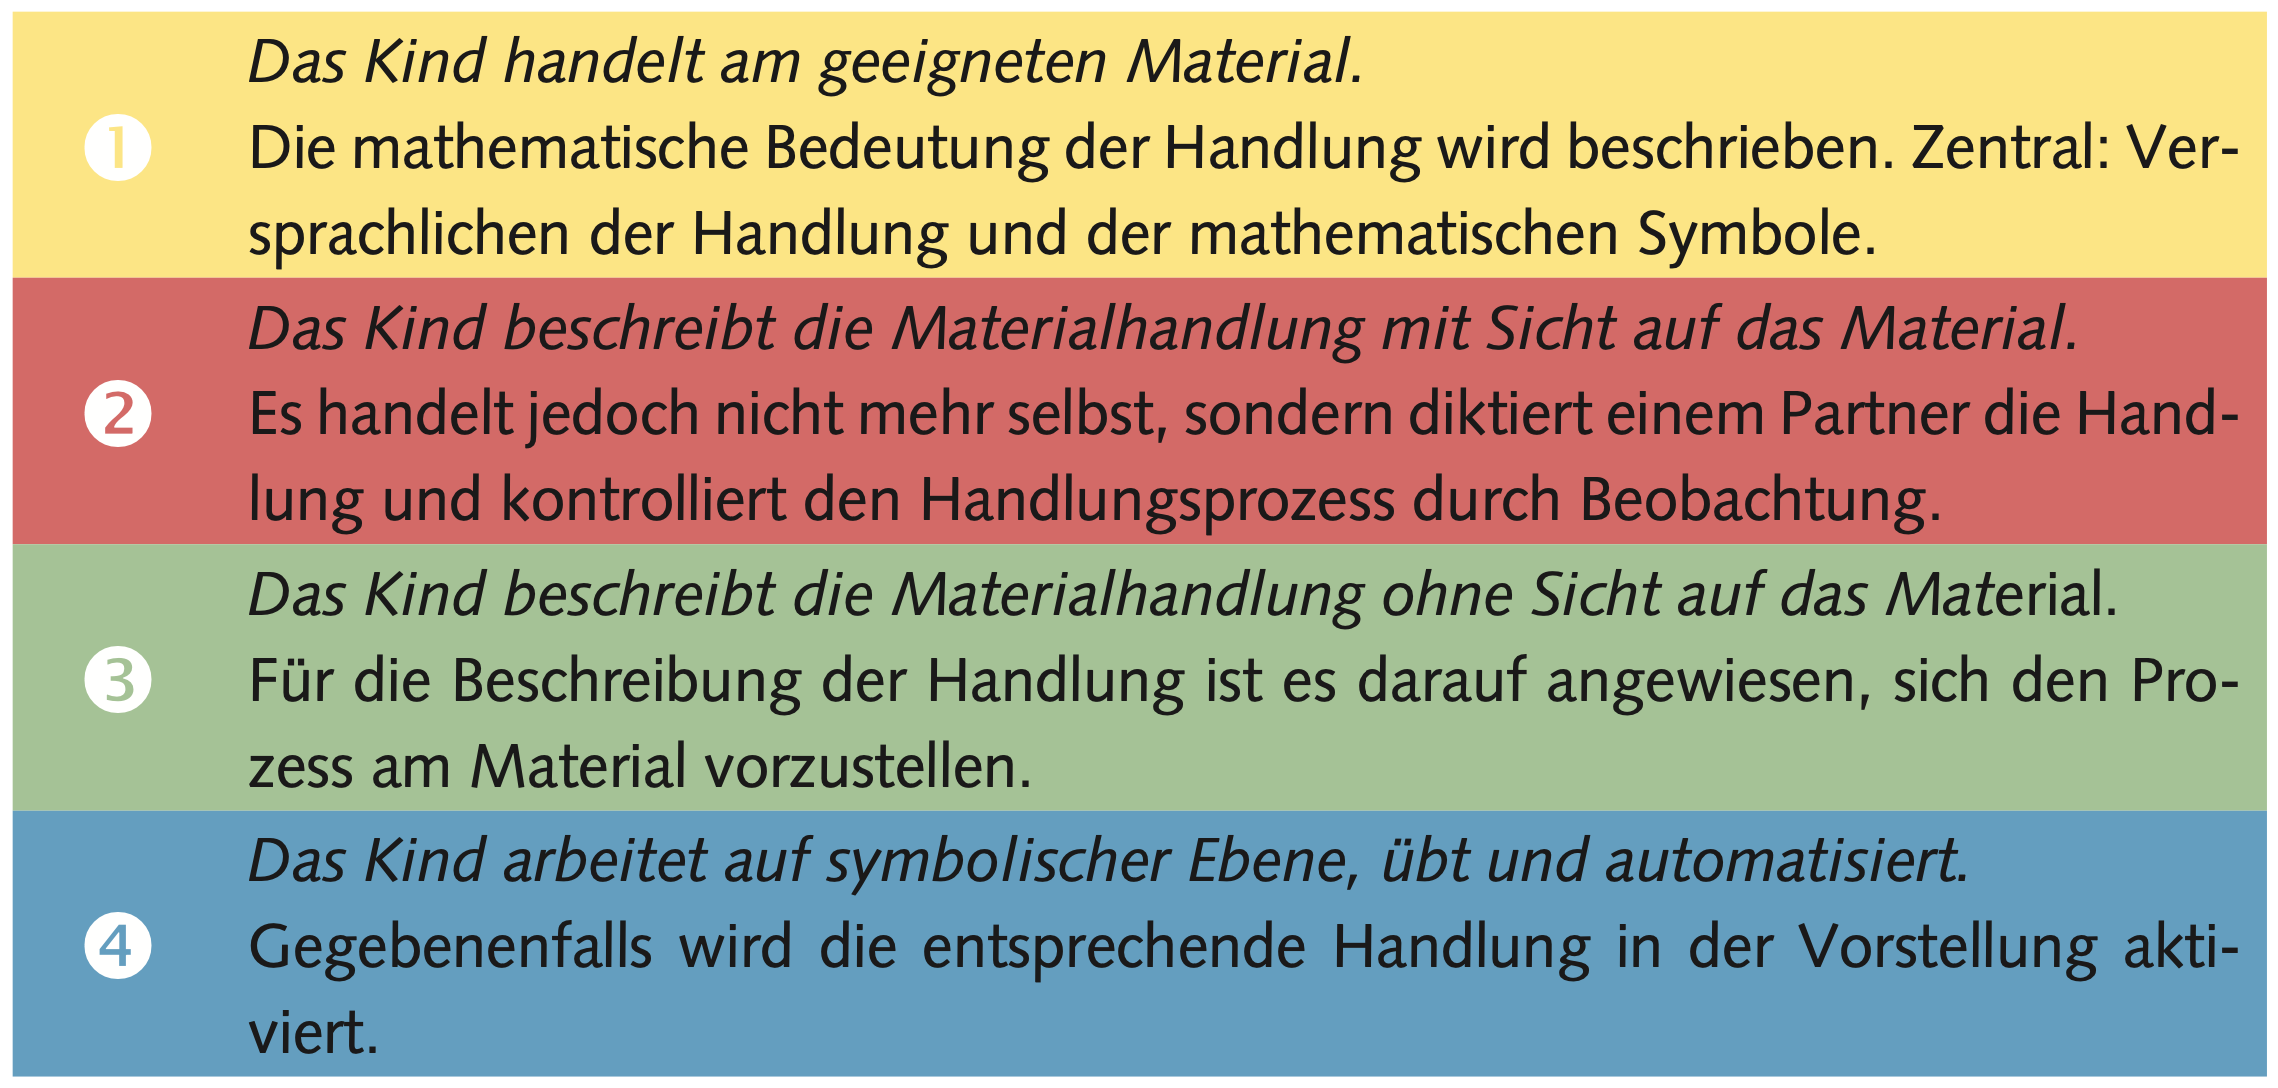
\includegraphics[width=0.9\linewidth]{pictures/6-GVverinnerlichen} 

}

\caption{Aufbau von Grundvorstellungen nach Wartha \& Schulz (\protect\hyperlink{ref-Wartha2011}{2011, S. 11})}\label{fig:GVVerinnerlichen}
\end{figure}

Steinhöfel et al. (\protect\hyperlink{ref-Steinhofel1988}{1988}) stellen (für die zur Zeit der Publikation) typische Unterrichtssituationen dar und nennen hierzu einige Möglichkeiten zur etappenweise Verinnerlichungen von Lernhandlungen im Mathematikunterricht, siehe Abbildung \ref{fig:Etappen}.



\begin{figure}

{\centering 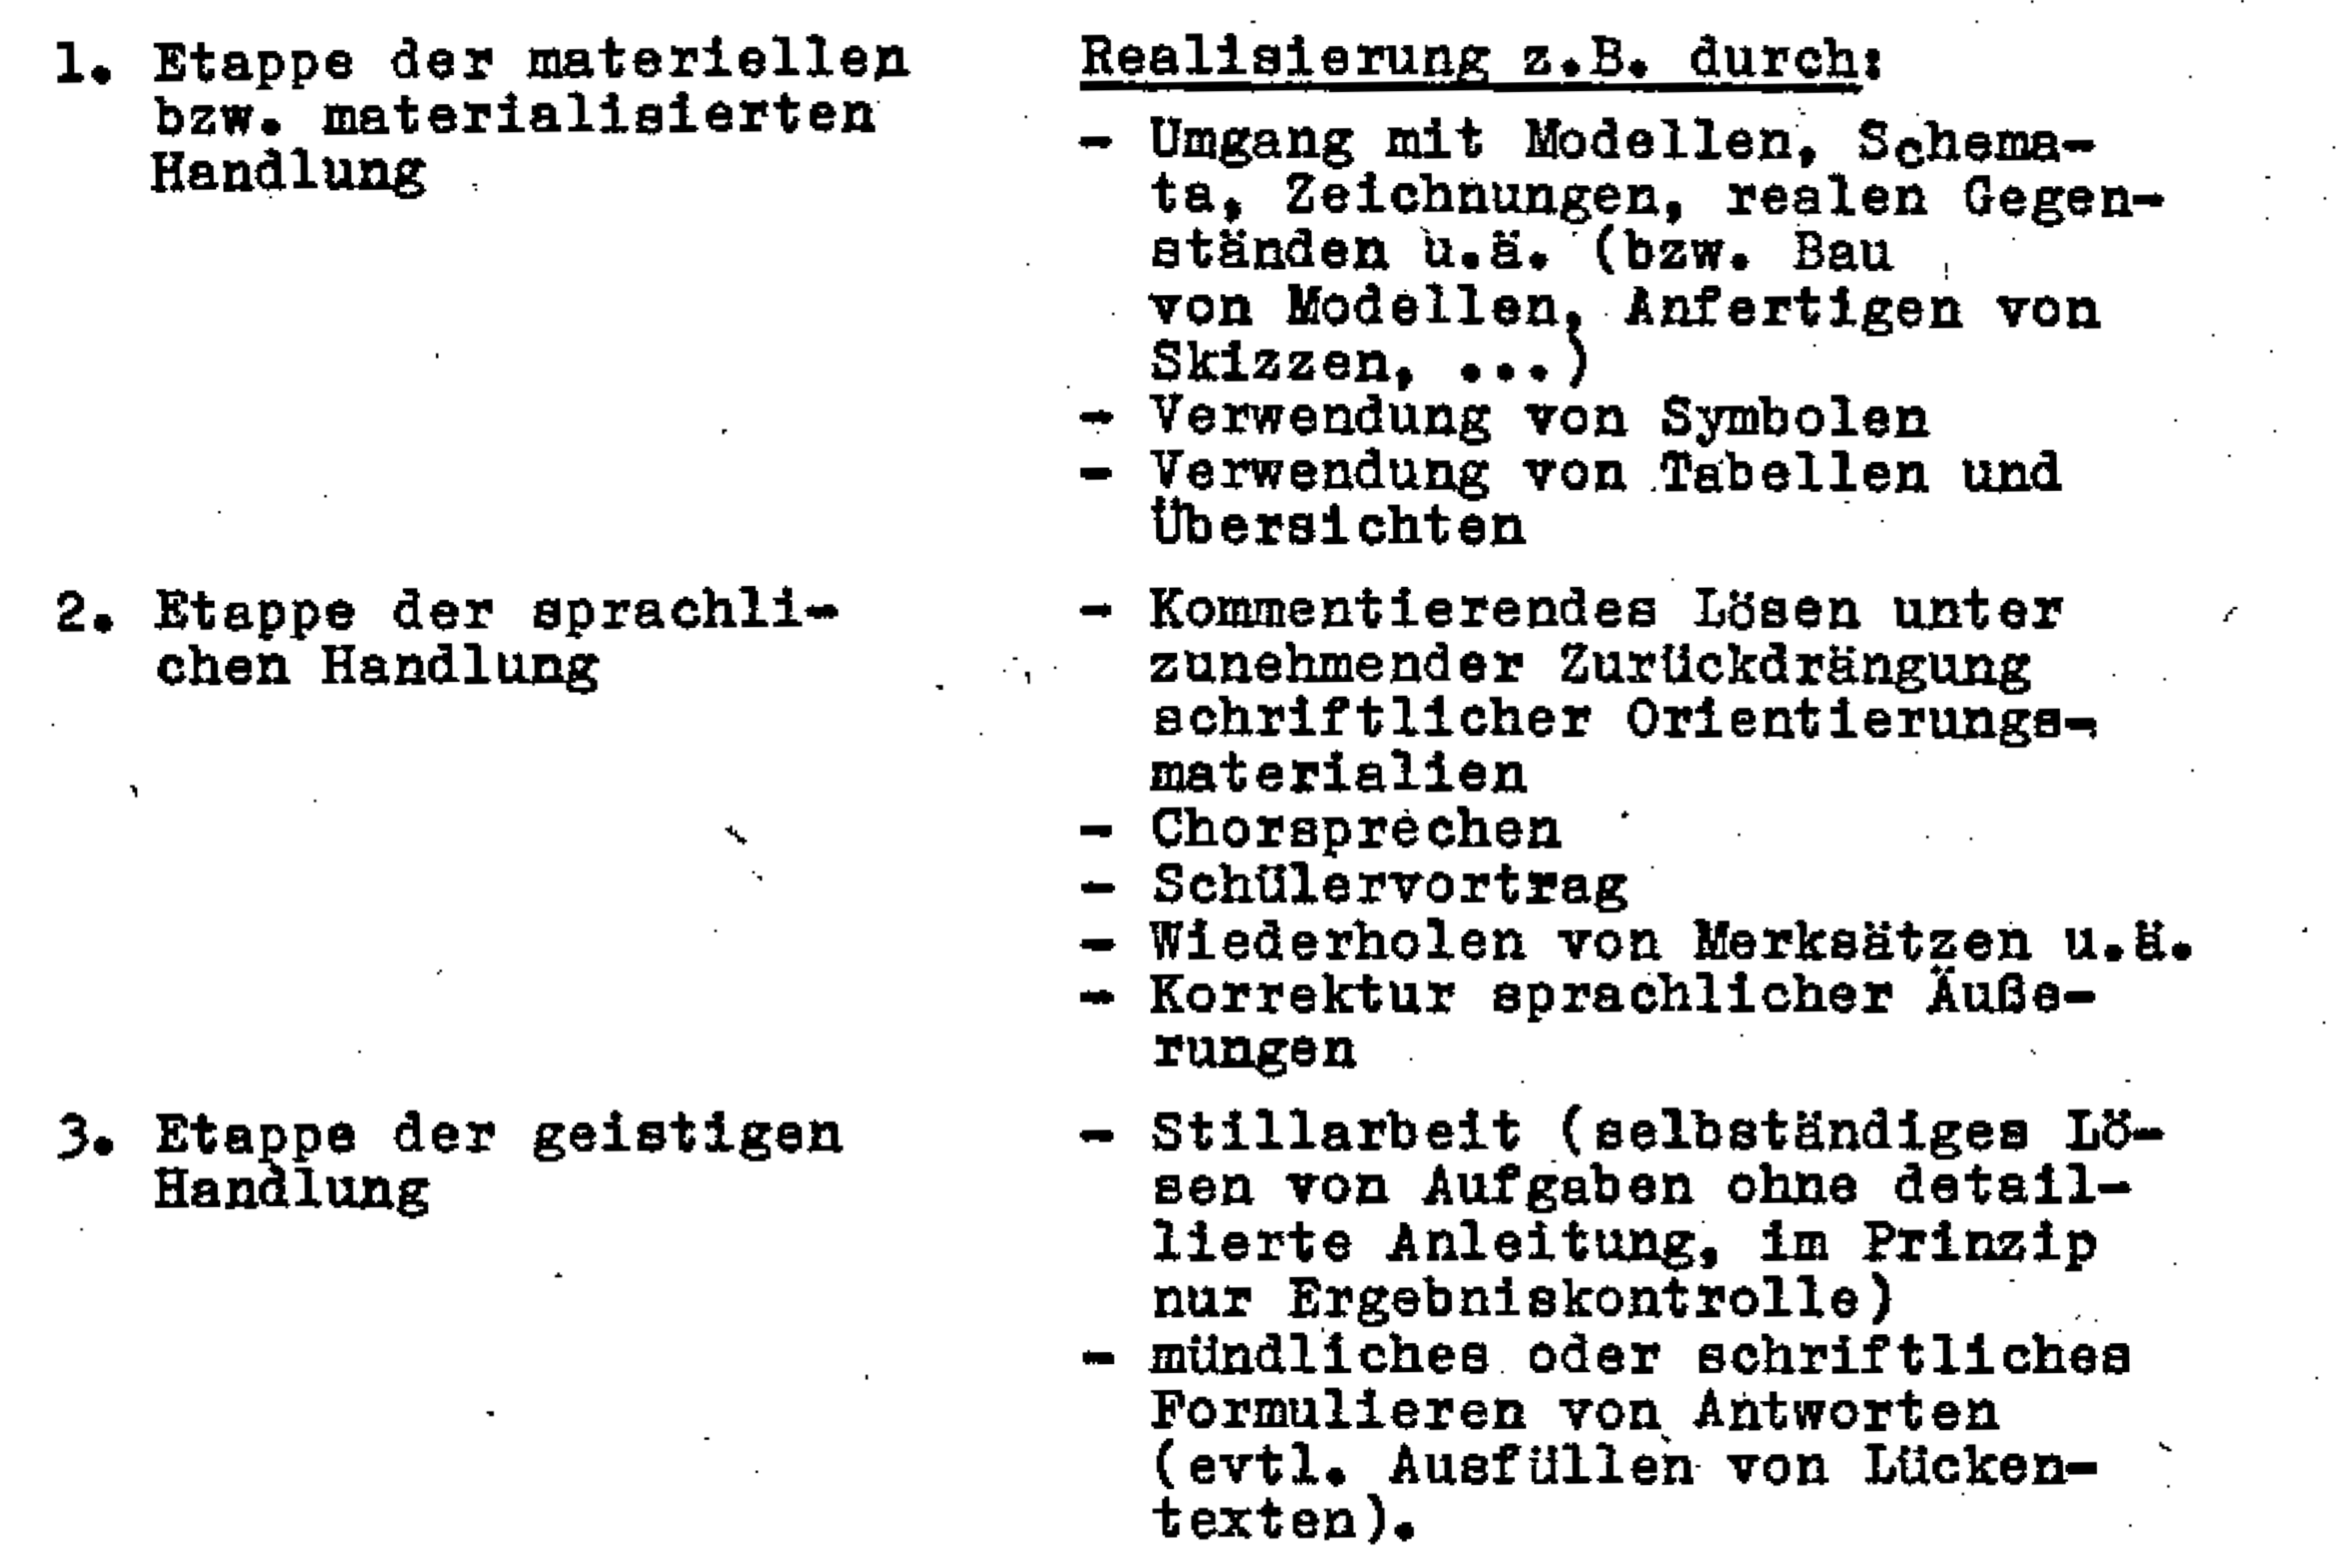
\includegraphics[width=0.9\linewidth]{pictures/6-Etappen} 

}

\caption{Beispiele zur etappenweisen Verinnerlichung von Handlungen im Mathematikunterricht nach Steinhöfel et al. (\protect\hyperlink{ref-Steinhofel1988}{1988, S. 19})}\label{fig:Etappen}
\end{figure}

\hypertarget{ordnenvertiefen}{%
\subsection{Ordnen/Vertiefen}\label{ordnenvertiefen}}

Die Handlungsausführung sollte stets von einer \textbf{Handlungskontrolle} begleitet werden. Das bedeutet, dass die Schülerinnnen und Schüler eine bewusste Beziehung herstellen zwischen ihren (erreichten oder zu erreichenden) Handlungsergebnissen, den eingesetzten Lernmitteln sowie deren Bedingungen und der eigenen Handlungsausführung.
Die Handlungskontrolle ist dabei eine \emph{Selbstkontrolle} und muss dementsprechend auch erst einmal ausgebildet werden. Folgende methodischen Maßnahmen scheinen hierfür hilfreich zu sein:

\begin{itemize}
\item
  Ein Abgleich mit den zu erreichenden Handlungsergebnissen ist nur möglich, wenn im Vorfeld eine Zielklarheit besteht. Es ist daher zu empfehlen, die \textbf{Lernziele} (siehe \ref{anknuepfen}) \textbf{explizit zu formulieren und auch festzuhalten}.
\item
  Durch das \textbf{Anfertigen eines Lernprotokolls} (vgl. \protect\hyperlink{ref-Bruder2011}{Bruder, 2001}) erhalten die Schülerinnen und Schüler eine Möglichkeit, ihre eigenen Lernhandlungen zu dokumentieren und nachzuvollziehen. Insbesondere kann in diesem auch ohne jeglichen Bewertungsdruck dargestellt werden, wo man selbst als Schülerin oder Schüler noch Lücken sieht bzw. was man noch nicht verstanden hat.
\item
  Als weitere effektive Maßnahme in der Ausbildung der Handlungskontrolle hat sich die \textbf{gegenseitige Kontrolle der Schülerinnen und Schüler} als hilfreich herausgestellt. »Es läßt sich zunächst beim Partner leichter feststellen als bei sich selbst, inwieweit ein Handlungsergebnis bestimmten Zielkriterien entspricht, die Handlungsausführung anforderungs- und regelgerecht erfolgt, wo Abweichungen und Fehler liegen und worin die Ursachen dafür bestehen können« {[}Lompscher1983a 72{]}. Durch Verinnerlichung dieses Vorgehens kann dann schrittweise auch eine Selbstkontrolle erfolgen.
\end{itemize}

Die dargestellten Beispiele greifen mit dem Abgleich zwischen Handlungsergebnissen und -zielen auch die \textbf{Rückschauperspektive der Kernideen/Kernfragen} auf. Die Handlungskontrolle befähigt damit die Schülerinnen und Schüler langfristig dazu, eine Feldorientierung über den Lerngegenstand zu erlangen.

\hypertarget{lerntaetigkeit-nachbereitung}{%
\section{Zum Nachbereiten}\label{lerntaetigkeit-nachbereitung}}

\begin{enumerate}
\def\labelenumi{\arabic{enumi}.}
\item
  Formulieren Sie eine Anforderungssituation in der Zone der nächsten Entwicklung am Beispiel der Vierecksarten und stellen Sie dar, inwieweit diese zwar verstanden und nachvollzogen, aber noch nicht selbstständig gelöst werden kann.
\item
  Konkretisieren Sie einige der für den Mathematikunterricht typischen Lernhandlungen (siehe Abschnitt \ref{typische-lernhandlungen}) am Lerngegenstand \emph{Vierecksarten}.
\item
  Beschreiben Sie Möglichkeiten zur etappenweisen Verinnerlichung der bei 2. dargestellten Lernhandlungen.
\end{enumerate}

\hypertarget{arbeitsmittel}{%
\chapter{Arbeitsmittel}\label{arbeitsmittel}}

\begin{quote}
\textbf{Ziele}

\begin{itemize}
\tightlist
\item
  Sie können den Begriff des Arbeitsmittels in den Vier-Ebenen-Ansatz sowie tätigkeitstheoretisch einordnen.
\item
  Sie kennen ein Instrument zur Analyse von Arbeitsmitteln.
\item
  Sie sind, ggf. mit Unterstützung, in der Lage, Arbeitsmittel strukturiert zu analysieren.
\end{itemize}

\textbf{Material}

\begin{itemize}
\tightlist
\item
  Folien zur Vorlesung zu Arbeitsmitteln (\href{files/Stoffdidaktik-WiSe2223-Kap7.pdf}{pdf}, \href{files/Stoffdidaktik-WiSe2223-Kap7.key}{Keynote})
\end{itemize}
\end{quote}

\hypertarget{begriffskluxe4rung-und-einordnung}{%
\section{Begriffsklärung und Einordnung}\label{begriffskluxe4rung-und-einordnung}}

Ausgehend von den im letzten Kapitel dargestellten theoretischen Betrachtungen, kommt \emph{Lernmitteln} (siehe Abschnitt \ref{taetigkeitstheorie-und-lernen}) bzw. \emph{Material} (siehe Abbildung \ref{fig:GVVerinnerlichen}) eine bedeutsame Rolle in der Ausbildung und Verinnerlichung von Lernhandlungen zu. Die Begrifflichkeiten sind jedoch nicht gleichzusetzen, was in diesem Abschnitt genauer herausgearbeitet werden soll.

\emph{Lernmittel} haben eine allgemeineren Charakter und entstammen einer weiteren tätigkeitstheoretischen Annahme: Tätigkeiten erfolgen nach Wygotski (\protect\hyperlink{ref-Wygotski1985a}{1985}) niemals direkt zwischen einem Individuum (dem \textbf{Subjekt}) und dem zu betrachtenden Gegenstand (dem \textbf{Objekt}), sondern geschehen stets über ein \textbf{vermittelndes Werkzeug}. Ein solches Werkzeug kann eine Geste sein, die Sprache (als Beispiel für ein sogenanntes \emph{psychisches Werkzeug}), Abbildungen und Skizzen, aber eben auch \emph{echte} Werkzeuge wie Maschinen, Geräte und andere Hilfsmittel.

\begin{figure}

{\centering 
\includegraphics[width=0.75\linewidth]{pictures/7-SubjektObjekt} 

}

\caption{Werkzeuge als Vermittler in der Tätigkeitstheorie}\label{fig:SubjektObjekt}
\end{figure}

Durch die Nutzung eines geeigneten Werkzeugs ist das Subjekt damit einerseits in der Lage, sein eigenes Wissen zu \textbf{\emph{externalisieren}}, d.~h. das Werkzeug zielgerichtet so einzusetzen, dass auf das Objekt eingewirkt werden kann. Andererseits kann das Werkzeug auch dabei helfen, Eigenschaften des Objekts zu \textbf{\emph{internalisieren}}, indem die Werkzeugnutzung dazu führt, dass das Subjekt Kenntnisse über das Objekt gewinnt.

Im Rahmen der Lerntätigkeit sind solche (ggf. psychischen) Werkzeuge dann \emph{Lernmittel} und können vielfältigster Natur sein:

\begin{itemize}
\tightlist
\item
  Mithilfe eines \emph{Zirkels} können Kreise erzeugt werden, indem der Zirkel seiner Funktion entsprechend verwendet wird (Externalisierung der Kenntnisse über den Kreis). Die Gestaltung und Handhabe des Zirkels selbst vermittelt jedoch auch Wissen über den Kreisbegriff, so dass dieses in der Verwendung des Werkzeugs aufgebaut werden kann (Internalisierung des Wissens über den Kreis).
\item
  Die \emph{digitale Stellenwerttafel} ermöglicht es, das Stellenwertverständnis zu Zahlen aufzubauen und Zahlen entsprechend darzustellen. Durch das Verhalten der Anwendung (dass z.~B. ein Plättchen beim Verschieben von der Zehner- in die Einer-Spalte automatisch entbündelt wird) unterstützt diesen Aneignungsprozess (siehe \protect\hyperlink{ref-Kortenkamp2018a}{Kortenkamp et al., 2018}).
\item
  Auch \emph{Aufgaben} haben die Funktion eines (bedeutsamen!) Lernmittels, wenn sie als Aufforderung zum Lernhandeln aufgefasst werden (siehe Abschnitt \ref{funktionen-von-aufgaben}). An ihnen erarbeiten sich die Schülerinnen und Schüler bestimmte Elemente des Lerngegenstands und die Gestaltung der Aufgabe sowie die vorhandenen Kenntnisse der Schülerinnen und Schüler bestimmen den Verlauf und Erfolg der Lernhandlung.
\end{itemize}

Der \emph{Material}-Begriff dagegen ist enger als der Begriff des \emph{Lernmittels} und stammt nicht aus der Tätigkeitstheorie. Verbreiteter und konkreter fassbar in der Mathematikdidaktik ist hierfür auch der Begriff des \textbf{Arbeitsmittels}. Nach Krauthausen (\protect\hyperlink{ref-Krauthausen:2018}{2018, S. 310}) sind Arbeitsmittel im Mathematikunterricht Veranschaulichungsmittel (zum Illustrieren oder Visualisieren mathematischer Konzepte) oder Anschauungsmittel (d.~h. »Darstellungen mathematischer Ideen in der Hand der Lernenden {[}\ldots{]} zur (Re-)Konstruktion mathematischen Verstehens«). Entscheidend ist hierbei eine »aktivistische« Sichtweise, also dass die Schülerinnen und Schüler die Arbeitsmittel aktiv als »Denkwerkzeug« verwenden. Die Aufgabe der Lehrkraft ist es dabei, »in den sachgerechten Gebrauch ein{[}zu{]}führen und Hilfen (zur Selbsthilfe) im Umgang mit Anschauungsmitteln {[}zu{]} gewähren« (\protect\hyperlink{ref-Krauthausen:2018}{Krauthausen, 2018, S. 310}). Schmidt-Thieme \& Weigand (\protect\hyperlink{ref-Schmidt-Thieme2015}{2015, S. 461~f.}) formulieren in inhaltlich ähnlicher Weise: »Arbeitsmittel repräsentieren mathematische Objekte und erlauben zudem Handlungen oder Operationen mit diesen Objekten«.\footnote{Den Arbeitsmitteln werden hier \emph{Anschauungsmittel} entgegengestellt, jedoch in einer eher demonstrierenden Bedeutung (\protect\hyperlink{ref-Schmidt-Thieme2015}{Schmidt-Thieme \& Weigand, 2015, S. 466~f.}), was eher dem Begriff der \emph{Veranschaulichungsmittel} bei Krauthausen (\protect\hyperlink{ref-Krauthausen:2018}{2018, S. 310}) entspricht.}

In dieser Einordnung übernehmen Arbeitsmittel demnach die Aufgabe eines Lernmittels (auch wenn es weitere Lernmittel gibt, die keine Arbeitsmittel sind). In der obigen Aufzählung der Beispiele kann die \emph{digitale Stellenwerttafel} als Arbeitsmittel aufgefasst werden.

Um den Begriff des Arbeitsmittels anzureichern, soll ein weiteres aus der Tätigkeitstheorie stammendes Konzept aufgegriffen werden, nämlich das des \textbf{\emph{Lernmodells}}. Lernmodelle sind »sinnliche Stützen geistigen Handelns« (\protect\hyperlink{ref-Giest2006}{Giest \& Lompscher, 2006, S. 225}) und können bspw. Zeichnungen, strukturierte Darstellungen, digitale Anwendungen usw. sein. Sie haben als Modelle dabei den Vorteil, dass sie »nicht die konkreten Merkmale der einzelnen Erscheinungen oder Situationen, sondern nur konstitutive, im gegebenen Kontext wesentliche Merkmale und Relationen enthalten, also \emph{abstrakt} sind« (\protect\hyperlink{ref-Lompscher1983a}{Lompscher, 1983a, S. 64}, Hervorhebung im Original). Gleichzeitig sind sie aber auch »\emph{anschauliche} Abbildungen und machen damit die grundlegenden Zusammenhänge und Wesensmerkmale der Wahrnehmung und Vorstellung zugänglich« (\protect\hyperlink{ref-Lompscher1983a}{Lompscher, 1983a, S. 64}, Hervorhebung im Original). Lernmodelle können daher insbesondere für mathematische Lerngegenstände dienlich sein, da sie die »abstrakte Struktur des Gegenstands zusammen mit dem prinzipiellen Weg {[}..{]}, der zur Aufdeckung der Struktur geführt hat«, beinhalten (\protect\hyperlink{ref-Lompscher1996}{Lompscher, 1996, S. 6}). Dass es sich dabei nicht ausschließlich um Abbildungen, sondern eben auch haptische Materialien oder digitale Anwendungen handeln kann, machen die obigen und noch folgenden Beispiele deutlich.

Bei der Entwicklung oder Auswahl eines Lernmodells ist es für Sie als Lehrkraft daher von besonderer Bedeutung, was der \emph{Kern} des entsprechenden mathematischen Gegenstands ist. Im Sinne der \textcolor{concreteColor}{konkreten Ebene} des Vier-Ebene-Ansatzes muss also das \textbf{Lernmodell mit der Kernidee in Einklang} stehen. Bezugnehmend auf die Grundvorstellungsidee (siehe Definition \ref{def:Grundvorstellungen}) auf der \textcolor{semanticColor}{semantischen Ebene} dienen damit \textbf{Lernmodelle als operationsfähige Repräsentationen} und erfüllen somit auch die Bedingungen an ein Arbeitsmittel.

Als Definition für Arbeitsmittel, die sowohl mathematikdidaktische als auch tätigkeitstheoretische Bezüge aufgreift, wird im Folgenden gewählt:

\begin{definition}[Arbeitsmittel]
\protect\hypertarget{def:Arbeitsmittel}{}\label{def:Arbeitsmittel}

Ein Arbeitsmittel ist eine \textbf{materielle oder materialisierte\footnote{Damit sind auch Abbildungen, Strukturdiagramme oder Apps eingeschlossen.} sowie operierbare Repräsentation} eines Lerngegenstands für die Hand der Schülerinnen und Schüler. Damit muss ein Arbeitsmittel folgende Bedingungen erfüllen:

\begin{itemize}
\tightlist
\item
  Es enthält kontextübergreifend die dem Wesen des Lerngegenstands entsprechenden Merkmale und Relationen \textbf{(Abstraktheit)}.
\item
  Es macht die dem Lerngegenstand zugrundeliegende Struktur der Wahrnehmung und Vorstellung zugänglich \textbf{(Anschaulichkeit)}.
\item
  Es ermöglicht, Lernhandlungen durchzuführen, die der Aneignung des Wesens des Lerngegenstands dienlich sind \textbf{(Operierbarkeit)}.
\end{itemize}

\end{definition}

\hypertarget{arbeitsmittel-analysieren}{%
\section{Arbeitsmittel analysieren}\label{arbeitsmittel-analysieren}}

\hypertarget{acat-modell}{%
\subsection{ACAT-Modell}\label{acat-modell}}

Als Lehrkraft werden Sie (wahrscheinlich) selten in der Situation sein, selbst Arbeitsmittel erstellen zu müssen. Bedeutsamer ist es, existierende Arbeitsmittel einschätzen und analysieren zu können --
gerade bei einer immer größer werdenden Fülle als digitalen Apps, die durchaus den Charakter eines Arbeitsmittels einnehmen können. Um Arbeitsmittel fundiert und strukturiert zu analysieren, bietet sich als Stütze das auf die Tätigkeitstheorie aufbauende Modell \textbf{Artifact-Centric Activity Theory (ACAT)}\footnote{übersetzt: Artefakt-zentrierte Tätigkeitstheorie} von Ladel \& Kortenkamp (\protect\hyperlink{ref-Ladel2013}{2013}) an, siehe Abbildung \ref{fig:ACAT}.



\begin{figure}

{\centering 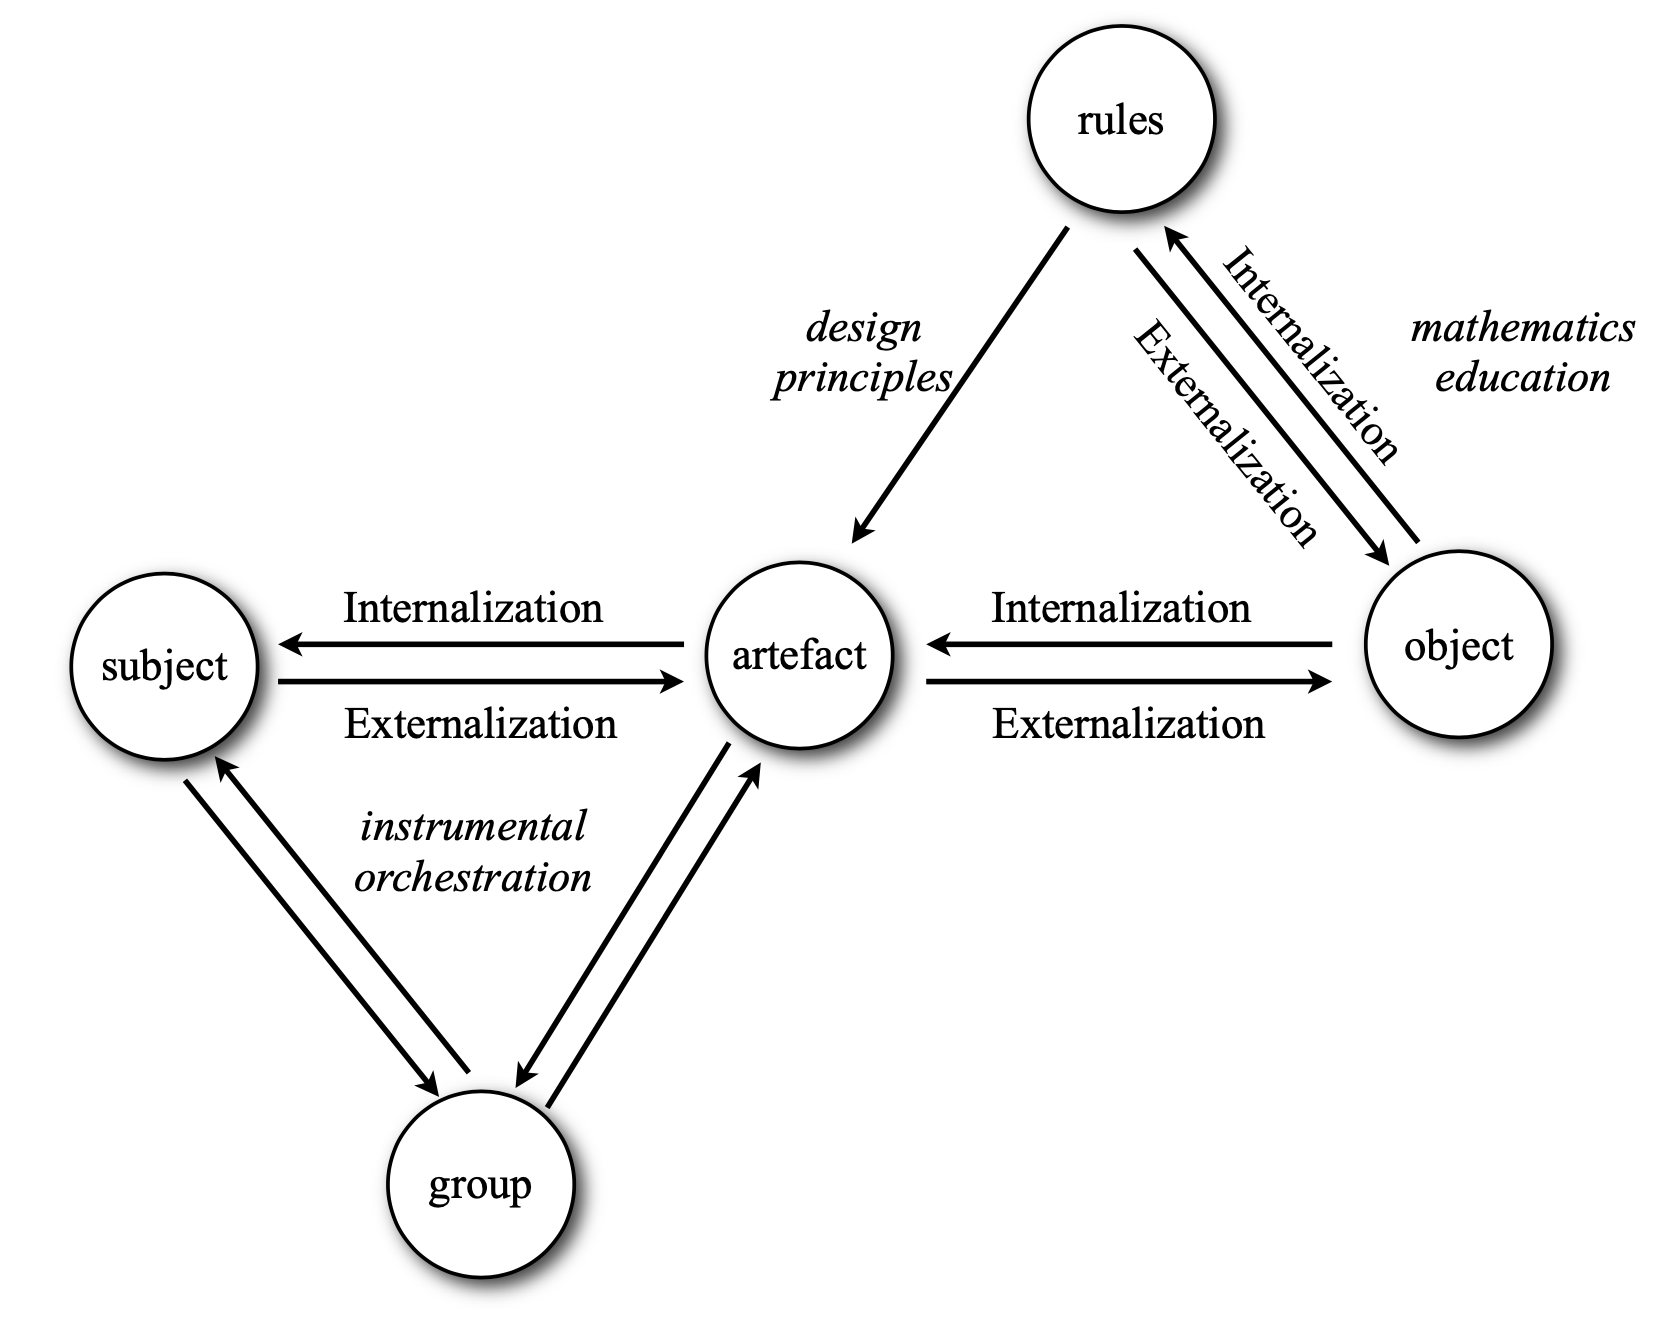
\includegraphics[width=0.75\linewidth]{pictures/7-ACAT} 

}

\caption{ACAT-Modell nach Ladel \& Kortenkamp (\protect\hyperlink{ref-Ladel2013}{2013, S. 4})}\label{fig:ACAT}
\end{figure}

Zunächst einmal ist auf der Hauptachse das Beziehungsgefüge aus Subjekt (Schüler/-in), Objekt (Lerngegenstand) und Artefakt (Arbeitsmittel) dargestellt, das der oben dargestellten Grundannahme der Tätigkeitstheorie entspricht.
Statt von einem Werkzeug ist hier von einem \emph{Artefakt} die Rede. Damit soll ausgedrückt werden, dass es sich um ein künstlich geschaffenes Medium handelt, das zum Zwecke des Wissenserwerbs von einer mit dem Lerngegenstand vertrauten Person (z.~B. Lehrkraft oder Forscherin bzw. Forscher) entwickelt worden ist. Erst mit dem tatsächlichen und zielgerichteten Einsatz durch die Schülerinnen und Schüler wird es zum \emph{Werkzeug}, weil erst dann Internalisierungs- und Externalisierungsprozesse stattfinden.\footnote{Die Entwicklung vom Artefakt zum Werkzeug wird auch als \emph{Instrumentelle Genese} bezeichnet (vgl. \protect\hyperlink{ref-Etzold2021}{Etzold, 2021, S. 101~f.}).} Diese \emph{Internalisierung- und Externalisierungsprozesse} werden hier im Modell auf der Hauptachse dargestellt.

Das obere rechte Dreieck beschreibt die spezifische Gestaltung des Artefakts über sogenannte \emph{Regeln}. Die Regeln ergeben sich einerseits aus dem mathematischen Gegenstand selbst. Andererseits stammen sie aus weiteren Wissenschaftsbereichen wie der Psychologie, allgemeinen Didaktik, Multimedia-Design usw. und wirken wieder zurück auf das mathematische Objekt, indem die Regeln einen Einfluss darauf haben, welche Eigenschaften des Objektes repräsentiert werden. Wenn beispielsweise ein Spielwürfel aus Design-Gründen abgerundete Ecken und Kanten hat (damit sich die spielenden Kinder nicht verletzen), kann sich dies auf ein (falsches) mathematisches Verständnis des Würfel-Begriffs auswirken. Daher ist ein solcher Spielwürfel ungeeignet als Arbeitsmittel für den Erstkontakt mit dem entsprechenden Begriff. Aus den Regeln heraus wird das Artefakt gestaltet.

Im unteren linken Dreieck wird nun der Einsatz des Artefakts in der \emph{Klassensituation} dargestellt. Hierbei spielen z.~B. konkrete Aufgabenstellungen eine Rolle, die die Schülerinnen und Schüler zur zielgereichteten Arbeit mit dem Artefakt anregen. Auch ist die Rolle der Lehrkraft im Lehr-Lern-Prozess von Bedeutung, ebenso wie die methodische Ausgestaltung der Artefakt-Nutzung, ggf. auch im Zusammenspiel mit weiteren Artefakten. Dieses komplexe Beziehungsgefüge wird auch als \emph{instrumental orchestration} bezeichnet (siehe z.~B. \protect\hyperlink{ref-Drijvers2010}{Drijvers et al., 2010, S. 214~f.}).

\hypertarget{analyseschritte}{%
\subsection{Analyseschritte}\label{analyseschritte}}

Larkin et al. (\protect\hyperlink{ref-Larkin2019}{2019}) stellen dar, wie sich das ACAT-Modell als Analyseinstrument für Unterrichtsapps einsetzen lässt, eine Übersetzung des Beurteilungsleitfadens findet sich bei Etzold et al. (\protect\hyperlink{ref-Etzold2018}{2018}) und eine für Lehrkräfte angepasste Variante bieten Kortenkamp et al. (\protect\hyperlink{ref-Kortenkamp2019}{2019}). Daran angelehnt bieten sich folgende Prozessschritte für die Analyse eines Arbeitsmittels an:

\begin{enumerate}
\def\labelenumi{\arabic{enumi}.}
\item
  \textbf{Identifizieren des mathematischen Objekts}

  Zunächst muss klar sein, für welches mathematische Objekt -- also für welchen Begriff, welchen Inhalt, welches Thema -- das Arbeitsmittel eingesetzt werden soll. Sind mehrere mathematische Objekte möglich, muss die Analyse auch für jedes getrennt erfolgen, da das Arbeitsmittel ggf. unterschiedlich gut geeignet sein kann. Theoretischer Hintergrund ist, dass \textbf{ohne Objekt keine zielgerichtete Handlung eines Subjekts möglich} ist. Daher können Handlungen von Schülerinnen und Schülern mit einem Arbeitsmittel nur dann bewertet werden, wenn Klarheit bezüglich des (mathematischen) Objekts besteht.

  \textbf{\emph{Mögliche Quellen}} hierfür sind die Bezeichnung des Arbeitsmittels bzw. eine offizielle Beschreibung, Zusatzmaterialien zum Arbeitsmittel (wie Arbeitsblätter, Handreichungen, \ldots), externe Referenzen (z.~B. Empfehlungen durch Dritte) oder auch das selbstständige Ausprobieren des Arbeitsmittels.
\item
  \textbf{Herausstellen der Interaktionsmöglichkeiten mit dem mathematischen Objekt über das Arbeitsmittel}

  Anschließend kann man sich Gedanken darüber machen, welche Interaktionsmöglichkeiten das Arbeitsmittel den Schülerinnen und Schülern mit dem mathematischen Objekt anbietet. Theoretischer Hintergrund hierfür ist, dass externe Handlungen des Subjekts (zum Beispiel eine \emph{pinch-to-zoom}-Geste zum Vergrößern oder Verkleinern einer Landkarte auf einem Tablet-Bildschirm) interne Handlungen wiederspiegeln (hier: zentrische Streckungen), die das Verständnis repräsentieren -- man spricht von \textbf{Externalisierung}. Ebenso führen externe Handlungen aber auch zum Aufbau interner Repräsentationen (hier z.~B.: Veränderung der Fingerposition zu Beginn der Handlung ändert das Streckungszentrum) -- man spricht von \textbf{Internalisierung}. Um diese Nutzerinteraktion besser zu verstehen und in Bezug auf das mathematische Objekt zu sehen, ist es hilfreich, den Prozess zwischen Subjekt und Objekt am Artefakt (dem Arbeitsmittel) aufzutrennen und in Teilfragen zu beantworten:

  \textbf{S → A:} Welche Handlungen sind mit dem Arbeitsmittel möglich?\\
  \textbf{A → O:} Wie repräsentiert das Arbeitsmittel das mathematische Objekt?\\
  \textbf{O → A:} Wie beeinflusst das Objekt das Verhalten des Arbeitsmittels?\\
  \textbf{A → S:} Welche Erfahrungen können Schülerinnen und Schüler dadurch machen?

  Eine \textbf{\emph{mögliche Quelle}} ist die eigene, systematische Nutzung des Arbeitsmittels.
\item
  \textbf{Analyse der Entwicklung der Interaktion}

  Nun werden die möglichen Interaktionen qualitativ strukturiert, um die mögliche Entwicklung des Lernens der Schülerinnen und Schüler besser zu beschreiben. Die Strukturierung bezieht sich auf die in der Tätigkeitstheorie übliche Unterscheidung in Tätigkeiten, Handlungen und Operationen:

  \begin{itemize}
  \tightlist
  \item
    \textbf{Tätigkeiten} sind übergeordnete, an \emph{Motiven} orientierte Interaktionen (z.~B. das Lesen einer Landkarte).
  \item
    \textbf{Handlungen} sind \emph{zielgerichtete}, individuelle Interaktionen, die die Tätigkeit realisieren (z.~B. das Vergrößern eines Kartenausschnittes, um diesen detaillierter betrachten zu können).
  \item
    \textbf{Operationen} sind zur Handlungsausführung notwendige Interaktionen, die jedoch kein weiteres Nachdenken erfordern und ggf. \emph{instrumentellen Zwängen} unterworfen sind (z.~B. das Ausführen der \emph{pinch-to-zoom}-Geste oder das Verschieben der Karte mit dem Finger).
  \end{itemize}

  In einem erfolgreichen Lernprozess verschieben sich (durch Verinnerlichungsprozesse) insbesondere Handlungen zu Operationen, um darauf neue, komplexere Handlungen aufbauen zu können. Es ist also darzustellen, wie eine dartige Entwicklung mithilfe des Arbeitsmittels unterstützt werden kann.

  \textbf{\emph{Mögliche Quellen}} sind hypothetische Diskussionen potenzieller Entwicklungen, aber auch empirische Untersuchungen.
\item
  \textbf{Überprüfung der Eignung des Arbeitsmittels für die Vermittlung des mathematischen Objekts}

  In diesem Schritt wird die Realisierung des Arbeitsmittels für das spezielle mathematische Objekt mit den Erkenntnissen aus Fachdidaktik, Fachwissenschaft und Psychologie verglichen. Dabei wird geprüft, ob die in den Schritten 2 und 3 analysierten Interaktionen tatsächlich die aus Sicht der Mathematik(-didaktik) erwünschten oder benötigten Vorstellungen, Erfahrungen und Kompetenzen unterstützen. Im ACAT-Modell entspricht dies der regelgeleiteten Gestaltung des Artefakts, wobei diese Regeln wiederum aus mathematikdidaktischen Überlegungen, allgemeinem Multimediadesign, usw. stammen.

  \textbf{\emph{Mögliche Quellen}} für diesen Schritt sind neben der Synthese der vorherigen Diskussionen v.~a. auch wissenschaftliche Referenzen und Veröffentlichungen.
\item
  \textbf{Möglichkeiten zur Verwendung des Arbeitsmittels in der Klassensituation }

  In einem letzten Schritt werden Möglichkeiten dargestellt, wie der Einsatz des Arbeitsmittels im Unterricht konkret aussehen kann. Folgende Fragen bieten eine Orientierung:

  \begin{itemize}
  \tightlist
  \item
    Ist das Arbeitsmittel für individuelle Arbeit, Partnerarbeit oder Kleingruppenarbeit geeignet?
  \item
    Was sind mögliche Impulse und Aufgabenstellungen, die Sie als Lehrerin oder Lehrer geben können?
  \item
    Welche Differenzierungsmaßnahmen und verschiedenen Schwierigkeitsgrade sind möglich?
  \item
    Handelt es sich um Übungsmaterial oder dient es zur Einführung neuer Lerninhalte und dem Aufbau von Grundvorstellungen?
  \item
    Welche Voraussetzungen/Kompetenzen werden an die Schülerinnen und Schüler für die Nutzung des Arbeitsmittels gestellt?
  \item
    Wie können Diskussionen bzw. Interaktionen innerhalb der Klasse mithilfe des Arbeitsmittels direkt oder indirekt gefördert werden?
  \end{itemize}

  Tätigkeitstheoretischer Hintergrund ist hierbei, dass Lernen niemals als eine rein individuelle Tätigkeit eines Schülers oder einer Schülerin angenommen wird, sondern immer im gesellschaftlichen und sozialen Kontext geschieht. Oder mit anderen Worten: »Im Unterricht agiert immer ein pädagogisches Gesamtsubjekt« (\protect\hyperlink{ref-Giest2004a}{Giest \& Lompscher, 2004, S. 112}).

  \textbf{\emph{Mögliche Quellen}} für derarbeite Überlegungen sind Materialien für Lehrerinnen und Lehrer, wissenschaftliche Ergebnisse, bspw. aus experimentellen Studien bzw. Versuchsdurchführungen im Unterricht.
\end{enumerate}

Diese fünf Schritte sprechen damit jeweils verschiedene Elemente des ACAT-Modells an. Abbildung \ref{fig:ACATAnalyse} fasst dies noch einmal zusammen.

\begin{figure}

{\centering 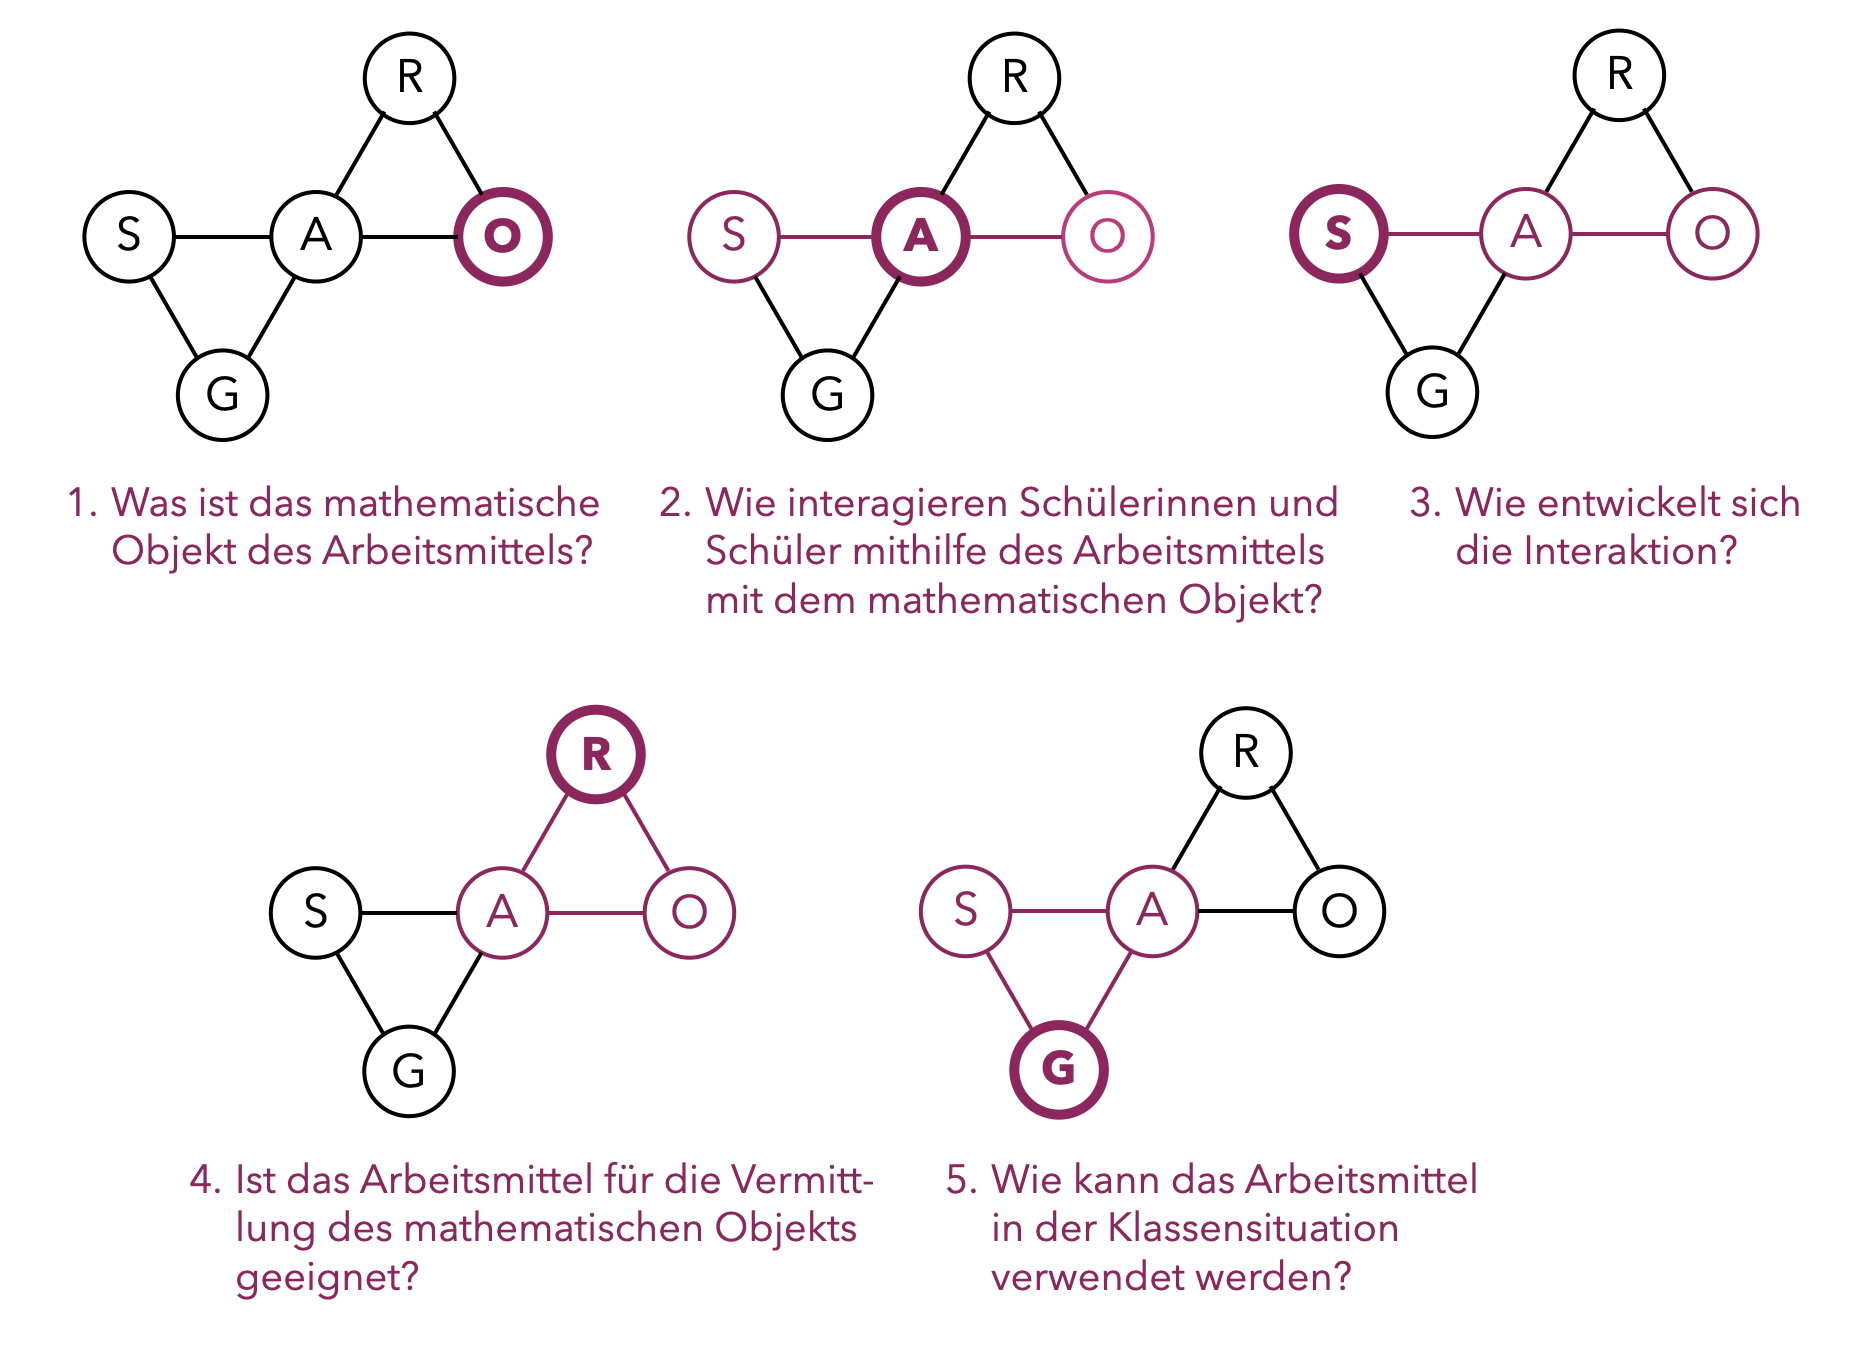
\includegraphics[width=0.9\linewidth]{pictures/7-ACATAnalyse} 

}

\caption{ACAT-Analysemodell für Arbeitsmittel}\label{fig:ACATAnalyse}
\end{figure}

Am Beispiel der App \emph{Klipp Klapp} (\protect\hyperlink{ref-Etzold2020a}{Etzold, 2020}) stellt Stein (\protect\hyperlink{ref-Stein2018}{2018}) eine entsprechende Analyse dar, die englischsprachige Übersetzung ist bei Larkin et al. (\protect\hyperlink{ref-Larkin2019}{2019, S. 85~ff.}) zu finden.

\hypertarget{arbeitsmittel-nachbereitung}{%
\section{Zum Nachbereiten}\label{arbeitsmittel-nachbereitung}}

\begin{enumerate}
\def\labelenumi{\arabic{enumi}.}
\item
  Lesen Sie als Hintergrundtheorie zur Analyse von Unterrichtsapps den Artikel von Larkin et al. (\protect\hyperlink{ref-Larkin2019}{2019}).
\item
  Führen Sie nach der hier vorgestellten Schrittfolge eine Analyse des Arbeitsmittels \emph{Zahlenstrahl} durch (siehe z.~B. auch \protect\hyperlink{ref-Schulz2018}{Schulz, 2018}).
\item
  Wählen Sie einen mathematischen Begriff und überlegen Sie sich, wie ein geeignetes Arbeitsmittel für diesen Begriff aussehen kann. Sie können dabei auch spekulieren, was dieses Arbeitsmittel können müsste (z.~B. wenn es digital umgesetzt werden könnte).
\end{enumerate}

\hypertarget{aufgabengestaltung}{%
\chapter{Aufgabengestaltung}\label{aufgabengestaltung}}

\begin{quote}
\textbf{Ziele}

\begin{itemize}
\tightlist
\item
  Sie kennen Möglichkeiten, Aufgaben je nach ihrer Funktion und den auszubildenden Fähigkeitsaspekten auszuwählen bzw. zu erstellen.
\item
  Sie können Aufgaben aus Schulbüchern für enstpechende Funktionen und Fähigkeitsaspekte anpassen.
\item
  Sie kennen Differenzierungsmöglichkeiten mithilfe von Aufgaben, insbesondere durch geeignete Hilfestellungen.
\end{itemize}

\textbf{Material}

\begin{itemize}
\tightlist
\item
  Folien zur Vorlesung zur Aufgabengestaltung (\href{files/Stoffdidaktik-WiSe2223-Kap8.pdf}{pdf}, \href{files/Stoffdidaktik-WiSe2223-Kap8.key}{Keynote})
\end{itemize}
\end{quote}

In der Veranstaltung \emph{Einführung in die Mathematikdidaktik} lern(t)en Sie zentrale Aufgabentypen kennen, die Ihnen Aussage über die \emph{Offenheit} von Aufgaben liefern (siehe auch \protect\hyperlink{ref-Bruder}{Bruder, o.~J., S. 2}). Weiterhin wird an dieser Stelle davon ausgegangen, dass Sie \emph{Operatoren} kennen, die für eine präzise Formulierung von Aufgabenstellungen genutzt werden können (siehe auch \protect\hyperlink{ref-InstitutfurQualitatsentwicklungimBildungswesen2019}{Institut für Qualitätsentwicklung im Bildungswesen, 2019}; \protect\hyperlink{ref-MinisteriumfurBildungJugendundSportdesLandesBrandenburg}{Ministerium für Bildung, Jugend und Sport des Landes Brandenburg, 2015, S. 11}). Dieses Kapitel soll Ihnen darauf aufbauend eine Sammlung unterrichtspraktischer Maßnahmen anbieten, Aufgaben zu gestalten. Explizite Bezüge zu tätigkeitstheoretischen Grundlagen finden Sie am Ende des Kapitels in Abschnitt \ref{theoretischer-rueckblick}.

\hypertarget{funktionen-von-aufgaben}{%
\section{Funktionen von Aufgaben}\label{funktionen-von-aufgaben}}

»Eine Aufforderung zum Lern-Handeln im Mathematikunterricht wird als \textbf{Aufgabe} bezeichnet« (\protect\hyperlink{ref-Bruder2012}{Bruder, 2012, S. 19}, Hervorhebung im Original). Mit diesem Aufgabenbegriff sind Sie nun als Lehrkraft gefordert, Ihre Schülerinnen und Schüler anzuregen, sich aktiv mit mathematischen Lerngegenständen auseinanderzusetzen. Dabei sollten Sie sich der verschiedenen möglichen \textbf{Funktionen von Aufgaben} bewusst sein, da dies jeweils die Art und Weise, wie Sie Aufgaben formulieren und sie im Unterricht einsetzen, beeinflussen (vgl. \protect\hyperlink{ref-Leuders2015}{Leuders, 2015, S. 439}; \protect\hyperlink{ref-SINUSBayern}{SINUS Bayern, o.~J.}). Die hier angebrachten Beispiele beziehen sich auf den Lerngegenstand \emph{Prozentrechnung}.











\begin{itemize}
\item
  Aufgaben können dem \textbf{Erkunden}, \textbf{Entdecken} und \textbf{Erfinden} dienen. Diese in der Regel am Anfang eines Themengebiets stehenden Aufgaben sollten möglich offen formuliert sein und in besonderer Weise Motivation schaffen, sich mit dem Lerngegenstand erstmals auseinanderzusetzen (siehe Abbildung \ref{fig:ProzentErkunden}). An dieser Stelle können auch typische W-Fragen gestellt werden -- es ist im Sinne der Offenheit nicht zwingend notwendig, sich an den Operatoren zu orientieren.

  \begin{figure}

    {\centering 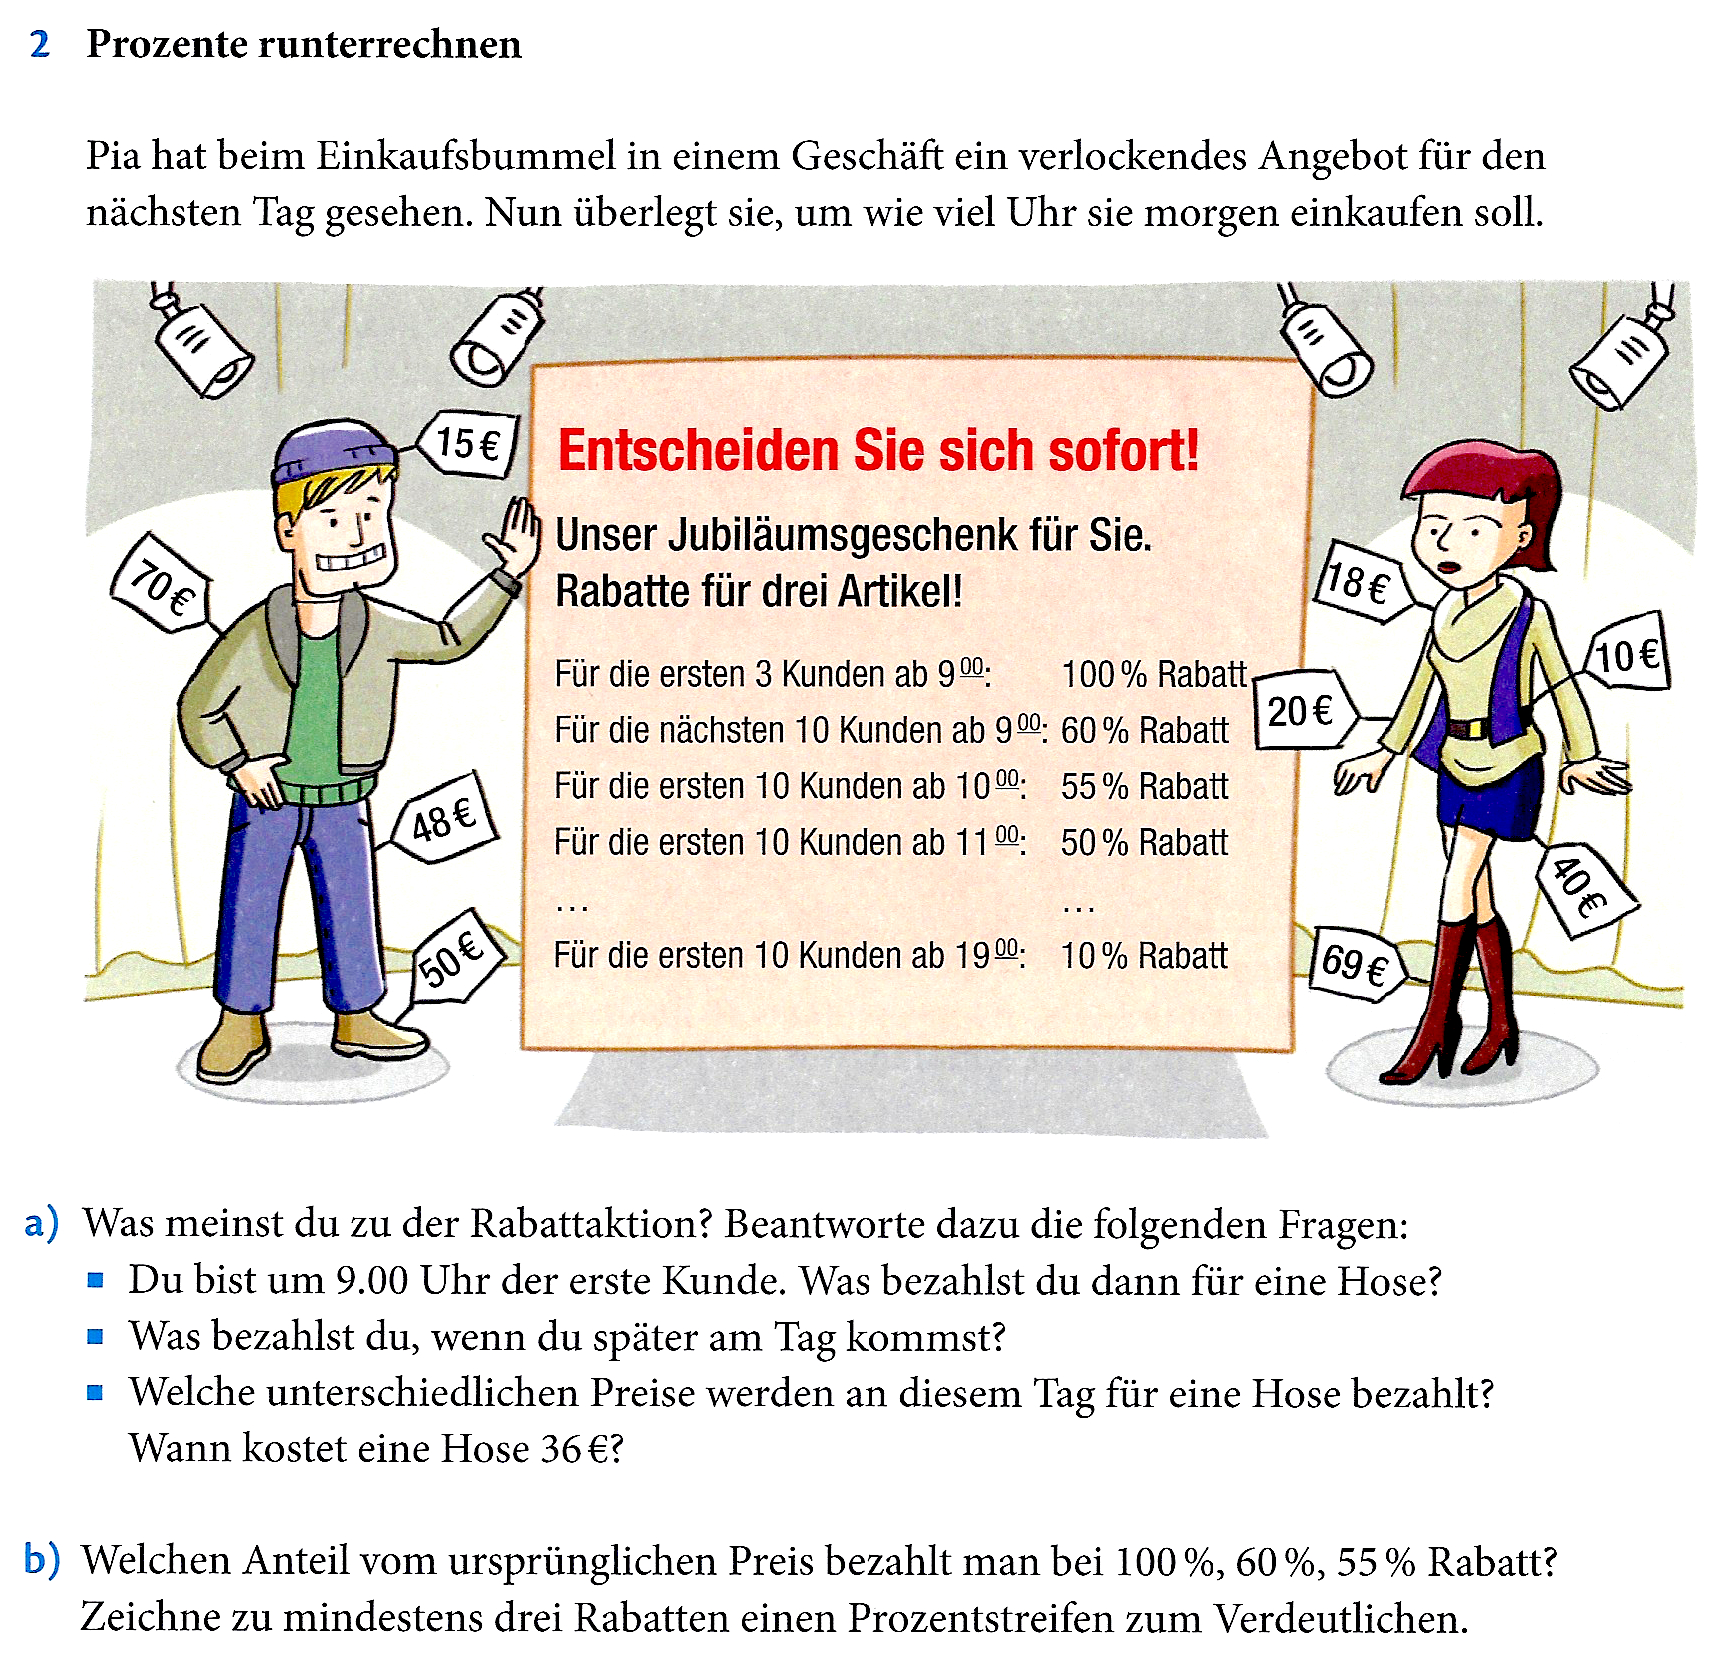
\includegraphics[width=0.75\linewidth]{pictures/8-ProzentErkunden} 

    }

    \caption{Erkundungsaufgabe zur Prozentrechnung (\protect\hyperlink{ref-Barzel2015a}{Leuders et al., 2015, S. 223})}\label{fig:ProzentErkunden}
    \end{figure}
\item
  Aufgaben zum \textbf{Sammeln}, \textbf{Sichern} und \textbf{Systematisieren} greifen vorherige Ideen auf, mit denen dann eine gewünschte mathematische Struktur herausgearbeitet werden soll (siehe Abbildung \ref{fig:ProzentSammeln}). In derartigen Aufgaben können Schülerinnen und Schüler auch angeleitet werden, sinnvolle Repräsentationen zu nutzen, um Grundvorstellungen auszubilden.

  \begin{figure}

    {\centering 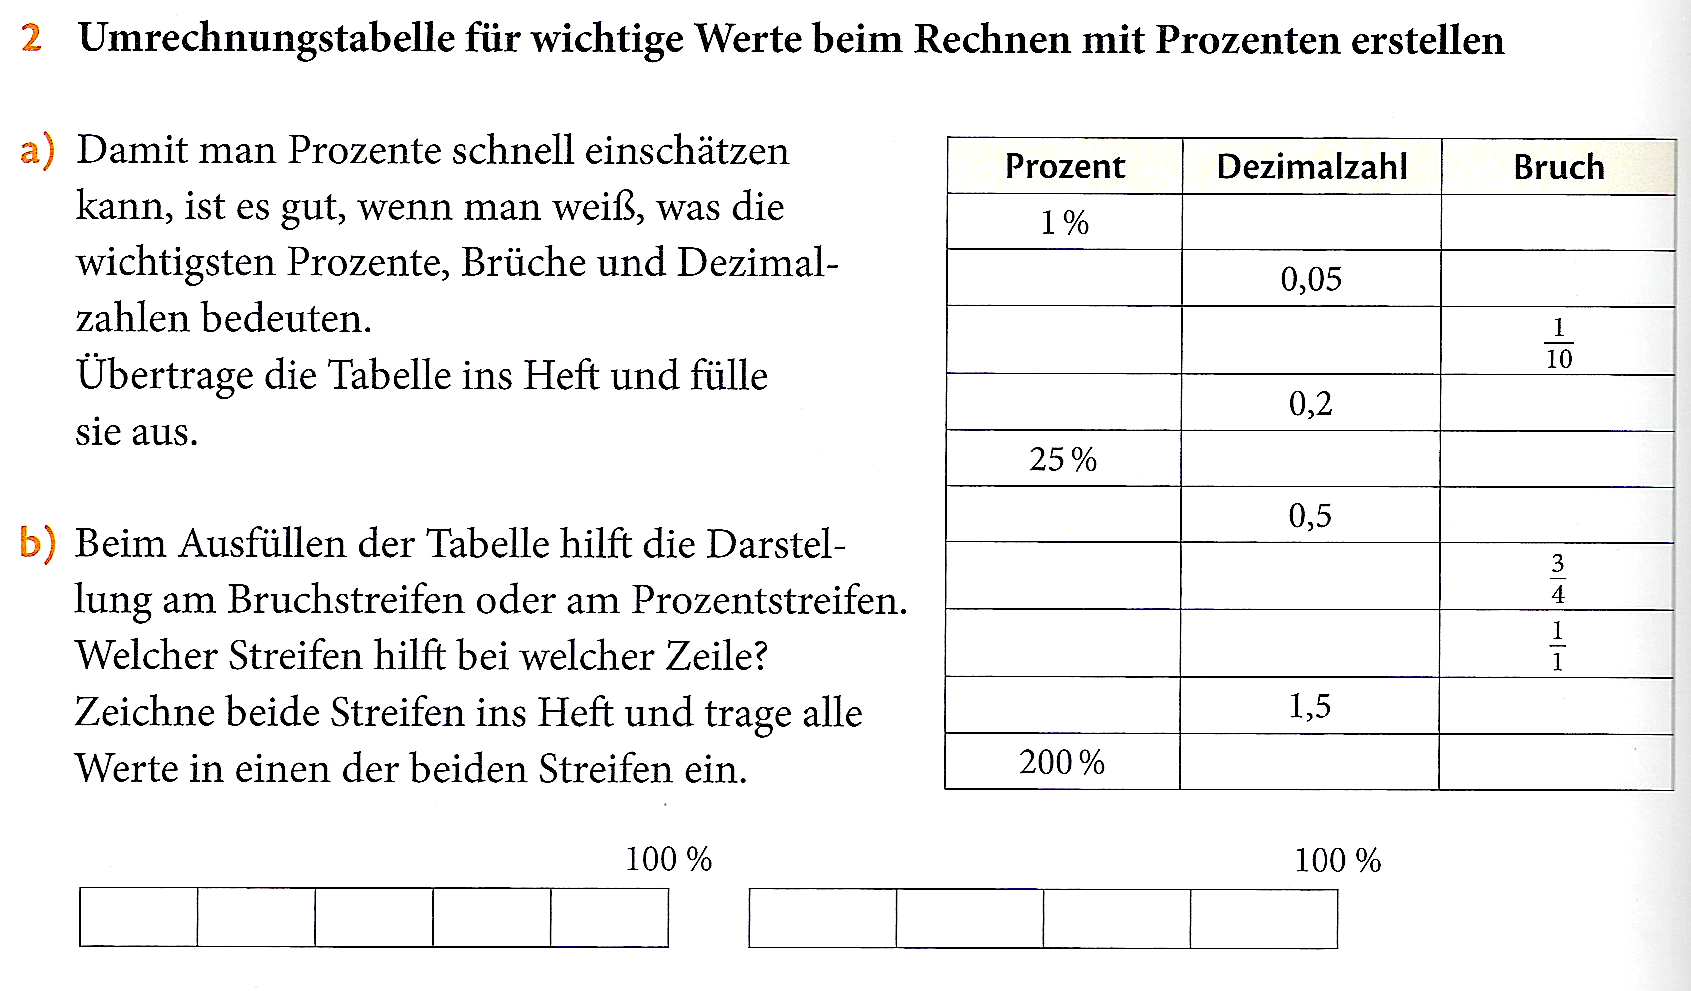
\includegraphics[width=0.75\linewidth]{pictures/8-ProzentSammeln} 

    }

    \caption{Systematisierungsaufgabe zur Prozentrechnung (\protect\hyperlink{ref-Barzel2015a}{Leuders et al., 2015, S. 226})}\label{fig:ProzentSammeln}
    \end{figure}
\item
  \textbf{Üben}, \textbf{Festigen} und \textbf{Wiederholen} sind weitere wesentliche Funktionen von Aufgaben im Mathematikunterricht. Hier sollten Sie eine möglichst große Vielfalt an Fähigkeitsaspekten ansprechen (siehe Abschnitt \ref{Faehigkeitsaspekte}), um sowohl Automatisierungsprozesse als auch den Transfer anzuregen. Sowohl geschlossene als auf teilweise geöffnete Aufgaben bieten sich hier an -- auch sind die verschiedenen Anforderungsbereiche anzusprechen, was sich in einer gezielten Auswahl an Operatoren widerspiegeln sollte (siehe Abbildung \ref{fig:ProzentUeben}).

  \begin{figure}

    {\centering 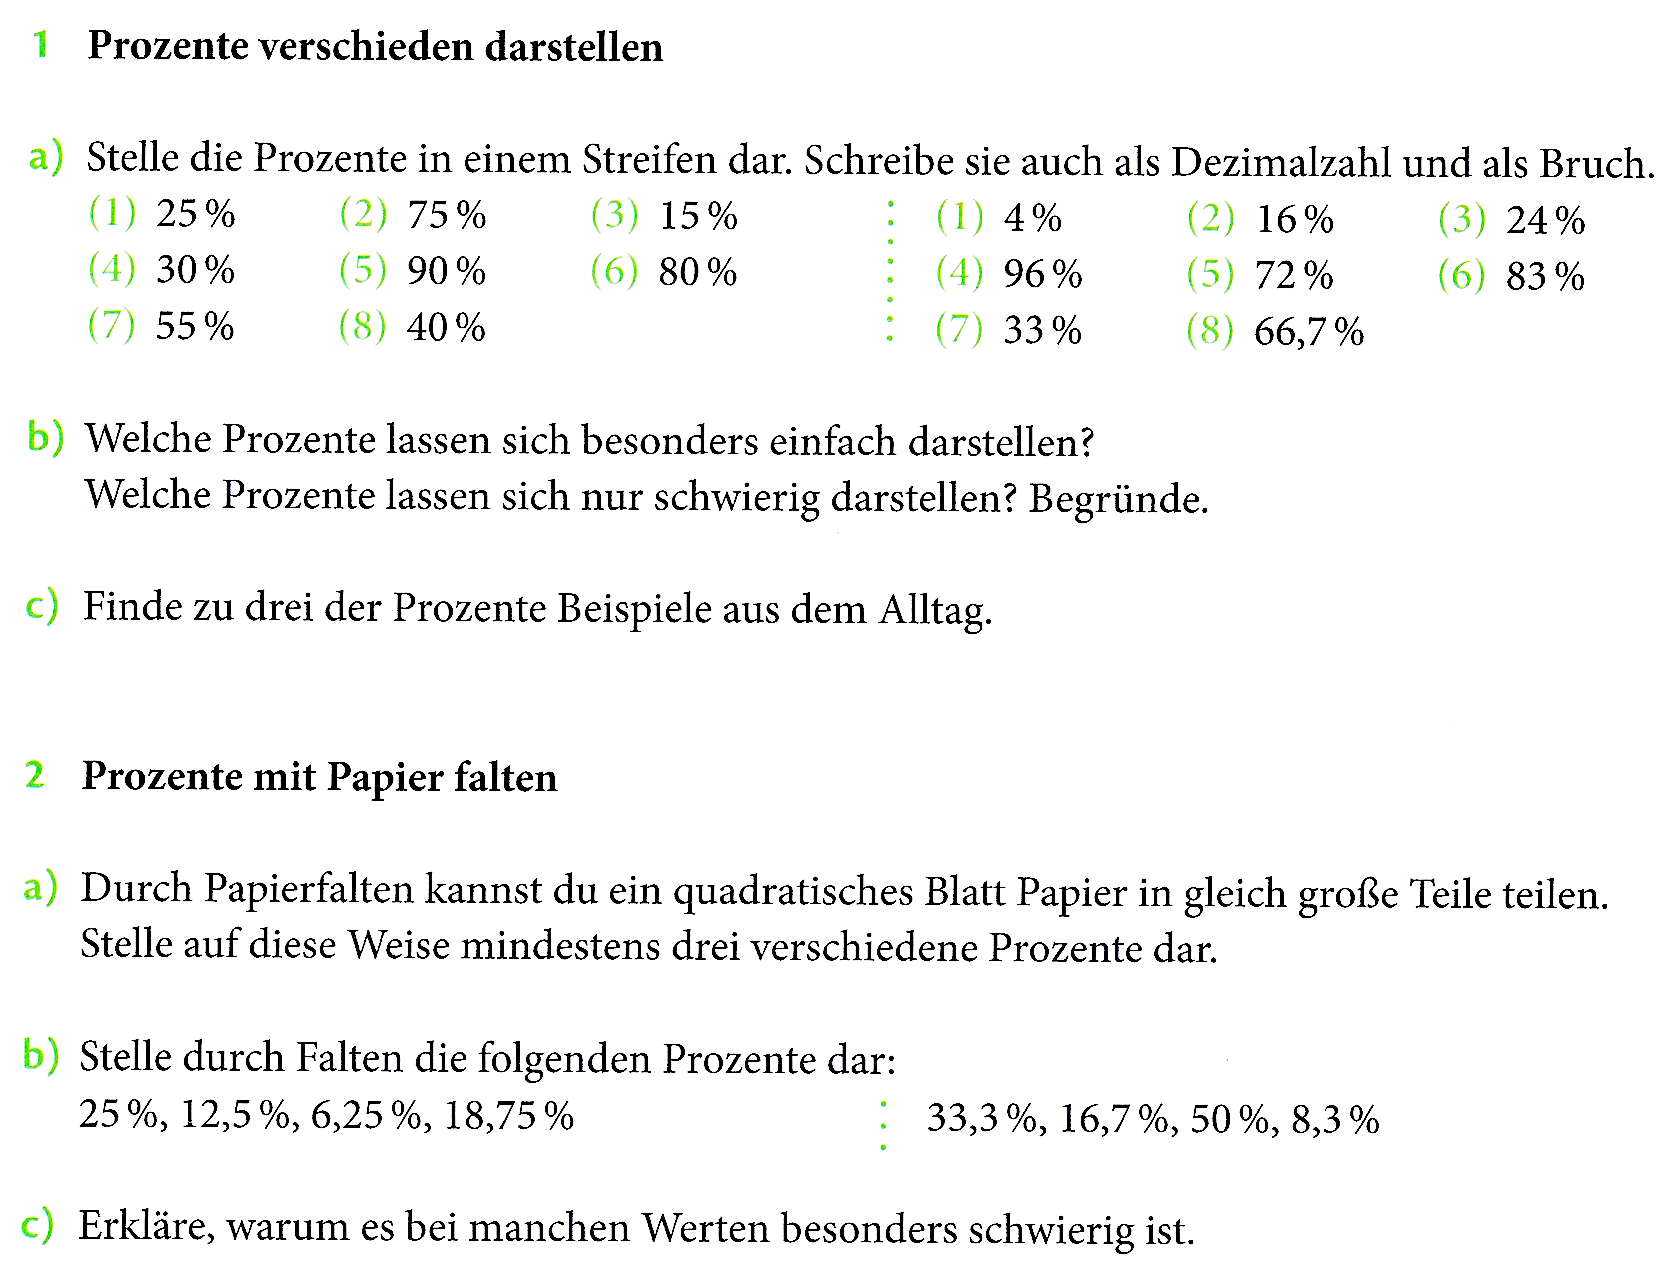
\includegraphics[width=0.75\linewidth]{pictures/8-ProzentUeben} 

    }

    \caption{Übungsaufgaben zur Prozentrechnung (\protect\hyperlink{ref-Barzel2015a}{Leuders et al., 2015, S. 232})}\label{fig:ProzentUeben}
    \end{figure}
\item
  Das \textbf{Vertiefen}, \textbf{Strukturieren} und \textbf{Vernetzen} stärkt das Kompetenzerleben der Schülerinnen und Schüler. Die Aufgaben werden wieder offener und können mit anderen Lerngegenständen in Bezug gebracht werden. Auch können Sonder- oder Grenzfälle der bisher betrachteten Aufgaben nun verstärkt eine Rolle spielen (siehe Abbildung \ref{fig:ProzentVertiefen}).

  \begin{figure}

    {\centering 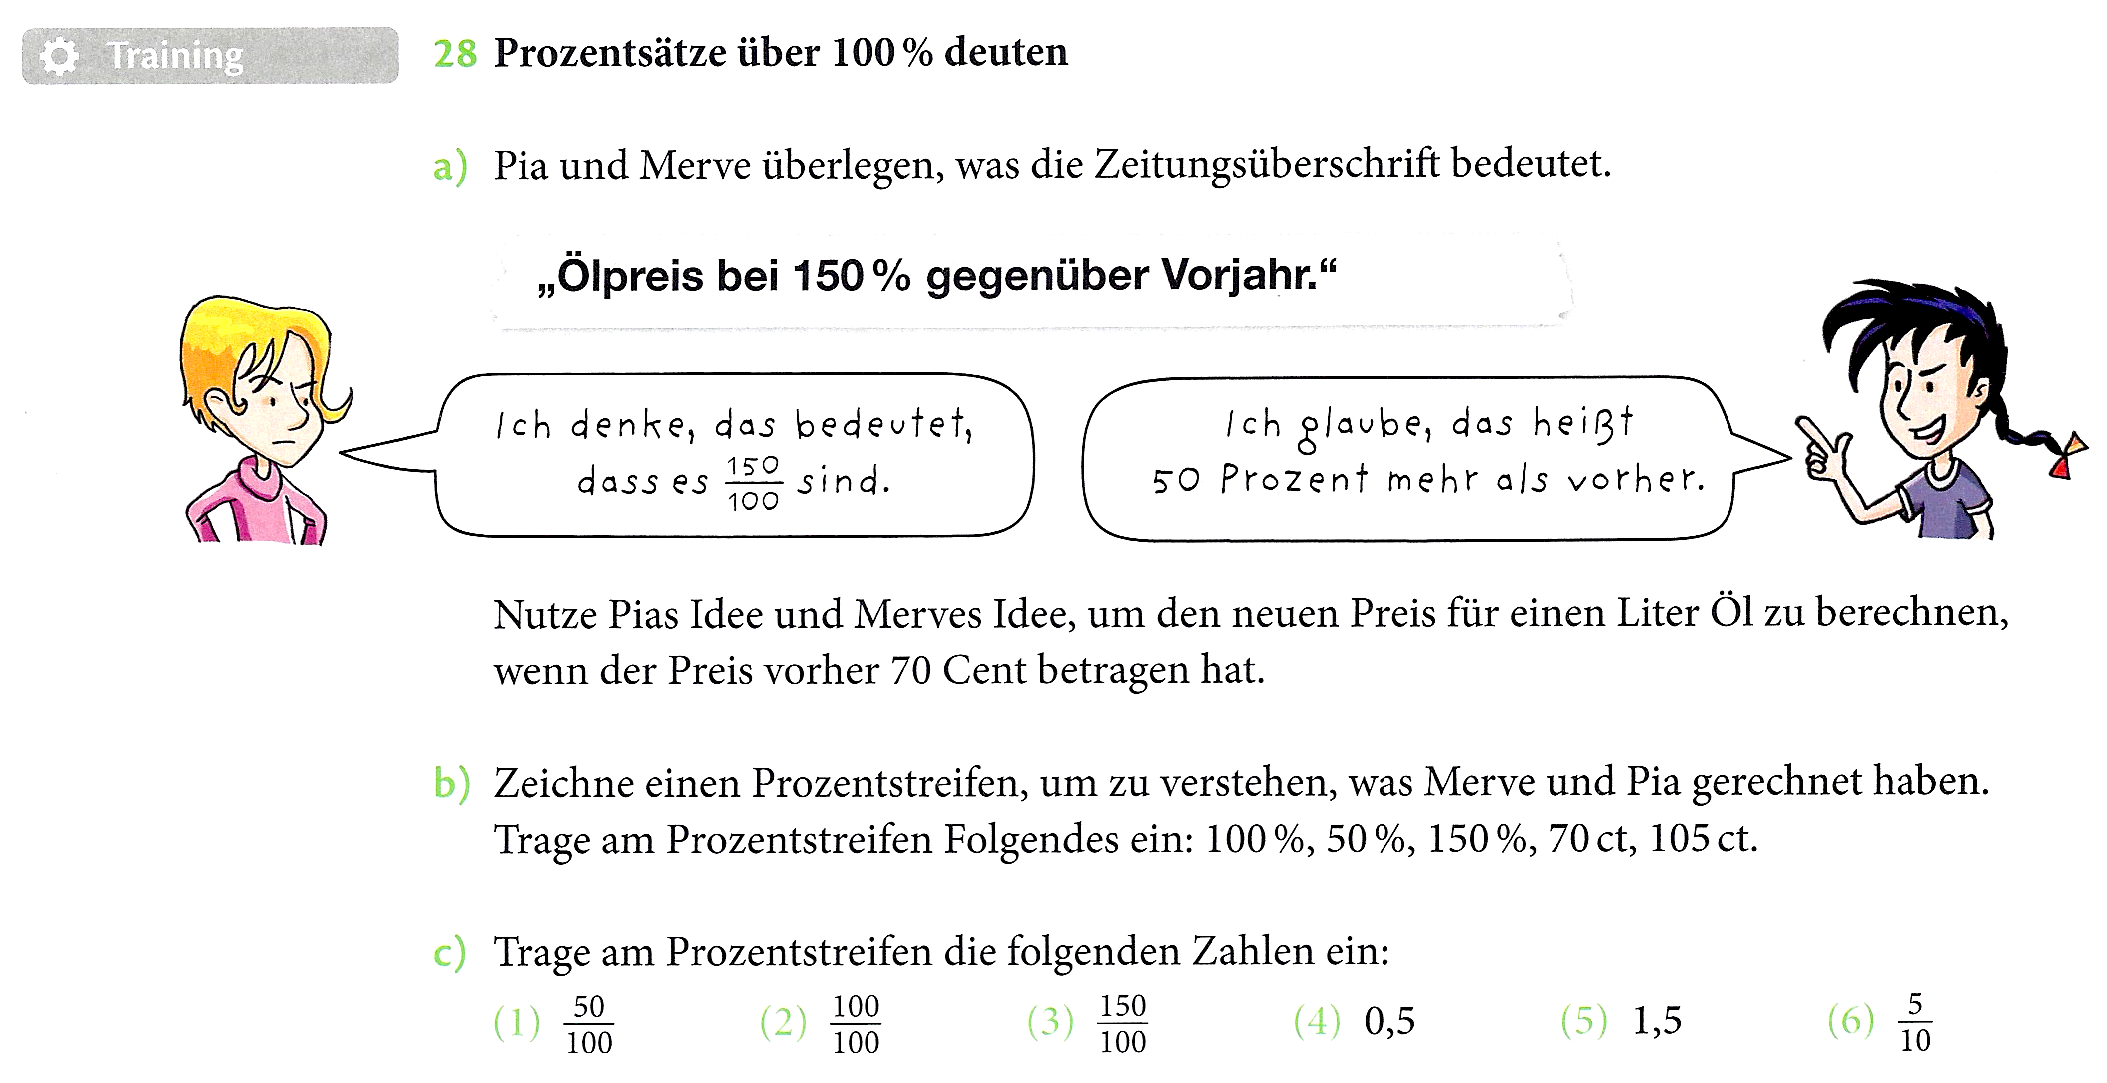
\includegraphics[width=0.75\linewidth]{pictures/8-ProzentVertiefen} 

    }

    \caption{Vertiefungsaufgabe zur Prozentrechnung (\protect\hyperlink{ref-Barzel2015a}{Leuders et al., 2015, S. 241})}\label{fig:ProzentVertiefen}
    \end{figure}
\item
  Die bisher genannten Funktionen hängen oftmals eng mit entsprechenden Unterrichtsphasen zusammen. Davon unabhängig können Aufgaben auch die Funktion des \textbf{Differenzierens} haben. Maßnahmen dafür werden in Abschnitt \ref{differenzieren} näher erläutert.
\item
  Weiterhin ist zwischen \textbf{Lernaufgaben} und \textbf{Leistungsaufgaben} zu unterscheiden. Letztere spielen bei der \textbf{Selbsteinschätzung}, \textbf{Diagnose} und \textbf{Leistungsmessung} eine besondere Rolle (siehe Abbildung \ref{fig:ProzentLeisten}). Insbesondere für solche Aufgaben sollten Operatoren genutzt werden, um die gewünschten Komptenzen gezielt überprüfen zu können, Erwartungen an die Schülerinnen und Schüler transparent zu machen und eine Vergleichbarkeit zu sichern.

  \begin{figure}

    {\centering 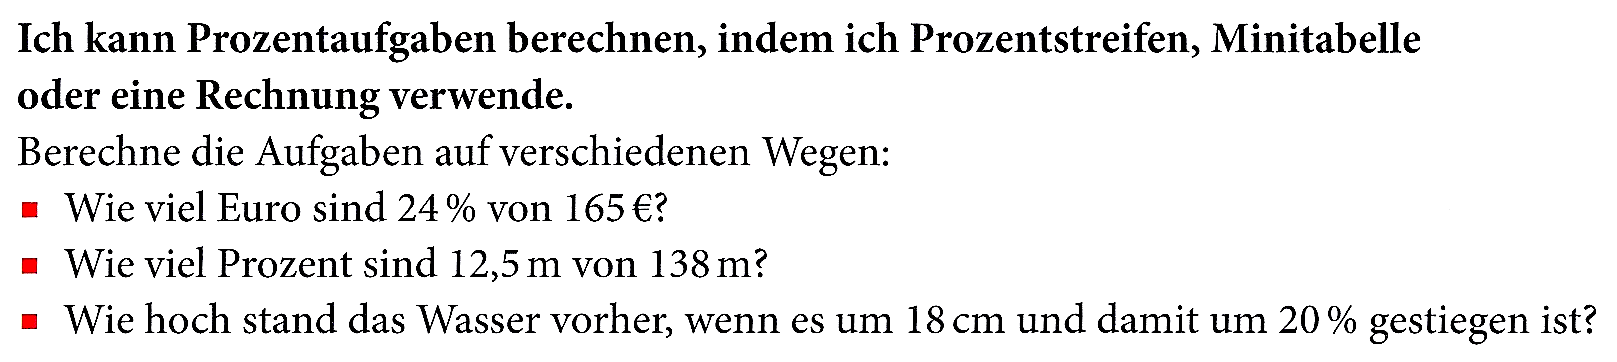
\includegraphics[width=0.75\linewidth]{pictures/8-ProzentLeisten} 

    }

    \caption{Selbsteinschätzungsaufgabe zur Prozentrechnung (\protect\hyperlink{ref-Barzel2015a}{Leuders et al., 2015, S. 244})}\label{fig:ProzentLeisten}
    \end{figure}
\end{itemize}

\hypertarget{produktives-uxfcben}{%
\section{Produktives Üben}\label{produktives-uxfcben}}

\hypertarget{Faehigkeitsaspekte}{%
\subsection{Fähigkeitsaspekte}\label{Faehigkeitsaspekte}}

Nicht selten wird man in Schulbüchern mit sogenannten \emph{Aufgabenplantagen} konfrontiert, also einer Vielzahl an Aufgaben immer derselben Art. Diese haben in der Regel das (berechtigte) Ziel, dass bestimmte Rechenoperation durch wiederholtes Üben automatisiert durchgeführt werden können. Im Schulalltag besteht jedoch die Gefahr, dass das Üben im Mathematikunterricht dann zum alleinigen \emph{Päckchenrechnen} verkommt, was der Vielzahl an \textbf{Fähigkeitsaspekten}, die ausgeprägt werden sollen, nicht gerecht wird.

Diese Fähigkeitsaspekte sind nach Leuders (\protect\hyperlink{ref-Leuders2009}{2009, S. 133}):

\begin{itemize}
\tightlist
\item
  \textbf{Kenntnisse}, es kann z.~B. die Definition eines math. Inhalts mit eigenen Worten wiedergegeben werden.
\item
  \textbf{Fertigkeiten}, es können z.~B. bestimmte Rechenoperationen durchgeführt werden.
\item
  \textbf{Verstehen/Vorstellungen}, es kann z.~B. an einem Bild der entsprechende math. Inhalt erklärt werden.
\item
  \textbf{Anwendungsfähigkeit}, es können z.~B. unbekannte Situationen mithilfe des math. Inhalts gelöst werden.
\item
  \textbf{(übergreifende) Strategien}, es können z.~B. Heurismen (vgl. \protect\hyperlink{ref-Kuzle}{Kuzle, o.~J.}) mithilfe des math. Inhalts angewandt werden.
\item
  \textbf{Reflexionsfähigkeit}, es kann z.~B. beurteilt werden, inwieweit der math. Inhalt in einer Situation relevant ist.
\item
  \textbf{Einstellungen}, es besteht z.~B. die Bereitschaft, sich mit dem math. Inhalt auseinanderzusetzen.
\end{itemize}

Diese Fähigkeitsaspekte sind nicht als Stufen aufzufassen, sondern gleichermaßen und unabhängig voneinander bedeutsam (\protect\hyperlink{ref-Leuders2009}{Leuders, 2009, S. 133}).

\hypertarget{aufgaben-veruxe4ndern}{%
\subsection{Aufgaben verändern}\label{aufgaben-veruxe4ndern}}

Einerseits sollten Sie als Lehrkraft in der Lage sein, zielgerichtet je nach Fähigkeitsaspekt Aufgaben auszuwählen. Andererseits, und das ist dann notwendig, wenn Sie keine guten Aufgaben finden, müssten Sie auch selbst welche entwickeln können -- was jedoch sehr zeitaufwendig ist. Ein in der Unterrichtspraxis effektiver Umgang ist das Verändern von existierenden Aufgaben, um diese \emph{produktiver} zu machen, d.~h. vielfältige Fähigkeitsaspekte anzusprechen.

Leuders (\protect\hyperlink{ref-Leuders2009}{2009, S. 137~ff.}) stellt in einer ausführlichen Tabelle (am Beispiel des arithmetischen Mittels) dar, wie man sich ausgehend vom gewünschten Fähigkeitsaspekt (z.~B. »Strukturen reflektieren«) und damit zusammenhängenden Aufgabentypen (z.~B. »Muster erkennen und erzeugen«) an geeigneten Fragetypen (z.~B.»Muster fortsetzen«) orientieren kann, um einen produktiven Umgang mit Aufgaben zu ermöglichen. Mit diesem Hintergrundwissen können Sie Ihren Blick auf existierende Schulbuchaufgaben richten und diese dann zielgerichtet anpassen.

Die soll am Beispiel einer Schulbuchseite zur Prozentrechnung dargestellt werden, siehe Abbildung \ref{fig:ProzentSchulbuch}.



\begin{figure}

{\centering 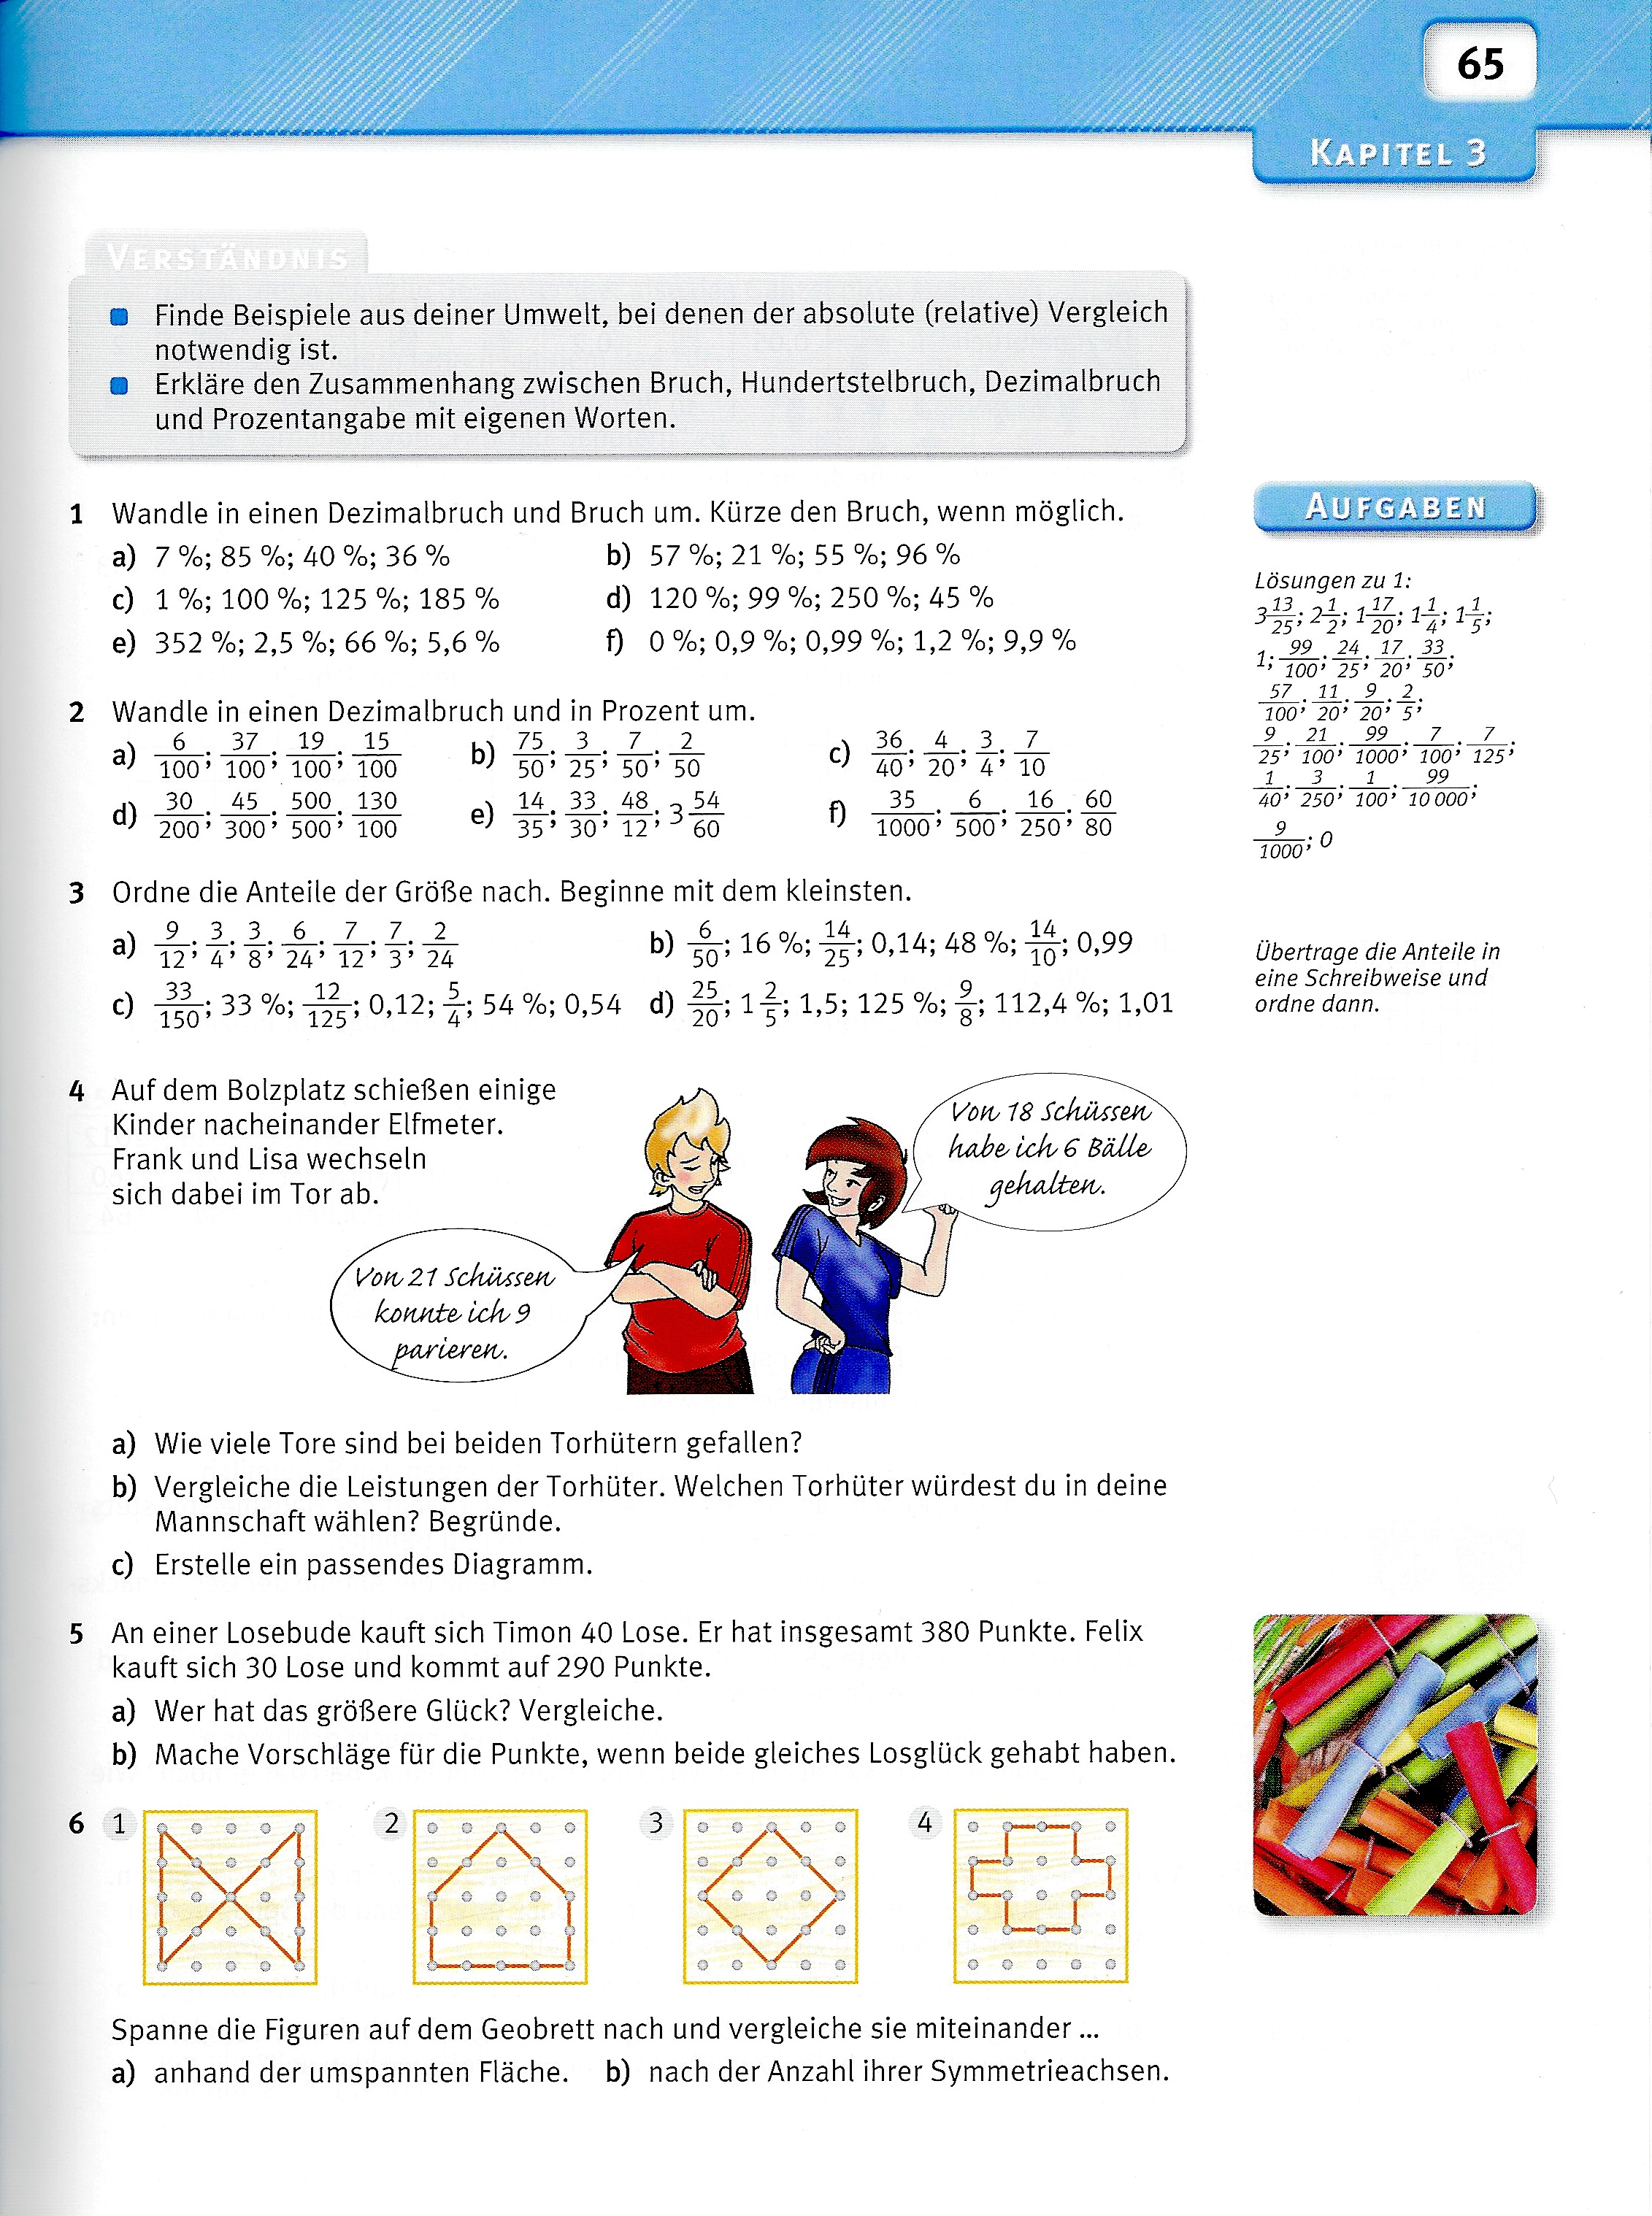
\includegraphics[width=0.75\linewidth]{pictures/8-ProzentSchulbuch} 

}

\caption{Schulbuchseite zur Prozentrechnung (\protect\hyperlink{ref-Kleine2011a}{Kleine \& Ludwig, 2011, S. 65})}\label{fig:ProzentSchulbuch}
\end{figure}

\begin{itemize}
\item
  Bei Aufgabe 2 könnte ergänzt werden:

  \emph{Welche Brüche lassen sich besonders leicht, welche schwerer in Dezimalbrüche und Prozent umrechnen? Woran liegt das?}

  Damit soll die Reflexion darüber angeregt werden, dass das Erweitern und Kürzen, sodass der Nenner 100 ergibt, je nach gegebenem Nenner unterschiedlich schwer sein kann. Hinsichtlich der Tabelle von Leuders (\protect\hyperlink{ref-Leuders2009}{2009, S. 138}) kann diese Aufgabe der Situation »Strukturen reflektieren« → »Strukturieren« → »Bewerten« zugeordnet werden. Statt alle Päckchen rechnen zu müssen, könnte nach der obigen Reflexion auch aufgefodert werden:

  \emph{Wähle eine leichte und eine schwere Teilaufgabe aus und löse sie.}
\item
  Aufgabe 3 ließe sich ergänzen durch:

  \emph{Wie ändert sich Lisas Leistung, wenn du weitere Schüsse aufs Tor zielst, die sie alle hält?}

  Diese Aufgabe betont den Zusammenhang zwischen Grundwert, Prozentwert und Protenzsatz, da jeder weitere Schuss sowohl den Grundwert als auch Prozentwert um 1 erhöht, womit zwar der Prozentsatz zunimmt, aber nicht linear steigt. Damit kann gleichzeitig eine tiefere Beschäftigung mit der dahinterliegenden arithmetischen Struktur angeregt werden. Nach Leuders (\protect\hyperlink{ref-Leuders2009}{2009, S. 137}) gehört diese Aufgabe zum Bereich »Probleme lösen« → »Operatives Durcharbeiten« → »Funktionale Abhängigkeit«.
\item
  Aufgabe 5 könnte ergänzt werden:

  \emph{Erfinde eine andere Situation, in der auf dieselbe Art und Weise gerechnet werden kann. Welche deiner Größen entsprechen den »Punkten« und der »Anzahl der Lose« und welche Rolle spielen diese Größen bei der Berechnung?}

  Hierüber wird eine strukturgleiche Übertragung der gegebenen Situation auf eine neue Situation gefordert. Dies führt dazu, sich tiefer mit dem Zusammenhang aus Rechenoperation und Anwendungskontext auseinanderzusetzen und entspricht bei Leuders (\protect\hyperlink{ref-Leuders2009}{2009, S. 139}) der Kategorie »Anwendungen erkunden« → »Anwenden« → »Anwendungen erfinden«.
\end{itemize}

\hypertarget{differenzieren}{%
\section{Differenzieren}\label{differenzieren}}

Um differenzierenden Unterricht zu ermöglichen, können Aufgaben entsprechend gestaltet werden. Dies kann mit \emph{leichten} und \emph{schweren} Aufgaben erfolgen -- es gibt aber noch weitaus mehr Möglichkeiten. Davon sollen hier einige exemplarisch vorgestellt werden, genauere Maßnahmen finden sich in den jeweils zitierten Quellen.

\hypertarget{gestufte-hilfen}{%
\subsection{Gestufte Hilfen}\label{gestufte-hilfen}}

Bei komplexen Aufgaben bietet es sich an, den Schülerinnen und Schülern gestufte Hilfen bereitzustellen, damit diese im Lösungsweg individuell unterstützt werden können (siehe auch \protect\hyperlink{ref-Zech1998}{Zech, 1998, S. 315~ff.}). Auch wenn Motivationshilfen (\emph{Die Aufgabe ist nicht so schwer.}), Rückmeldungshilfen (\emph{Du bist auf einem guten Weg.}) oder allgemeine strategische Hilfen (\emph{Lies die Aufgabe noch mal durch.}) deratige Unterstützungen sind, sollte bei der stoffdidaktisch-orientierten Unterrichtsplanung der Schwerpunkt auf \textbf{inhaltsorientierten strategischen Hilfen} sowie auf \textbf{inhaltlichen Hilfen} im Zusammenhang mit dem Lerngegenstand liegen.

\begin{itemize}
\item
  Inhaltsorientierte strategische Hilfen beziehen sich auf typische am Lerngegenstand orientierte Herangehensweisen zur Lösung einer Aufgabe. Mögliche Beispiele sind:

  \emph{Veranschauliche dir die Situation mit einer Skizze.}
  \emph{Stelle eine Gleichung auf.}
  \emph{Orientiere dich beim Vorgehen an dem Beispiel, das du bereits gerechnet hast.}
\item
  Inhaltliche Hilfen beziehen sich direkt auf die mit der Aufgabe verbundenen Begriffe, Regeln und Zusammenhänge. Dies können z.~B. sein:

  \emph{Überlege, was mit dem Flächeninhalt passiert, wenn du die Seitenlängen verdoppelst.}
  \emph{Du kannst hier das Kommutativgesetz anwenden.}
\end{itemize}

Zech (\protect\hyperlink{ref-Zech1998}{1998, S. 315}) betont, »nie mehr {[}zu{]} helfen als erforderlich«, um eine Aufgabe erfolgreich lösen zu können. Gestufte Hilfen haben demnach die Funktion, trotz ggf. vorhandener Schwierigkeiten Erfolgserlebnisse bei den Schülerinnen und Schülern zu ermöglichen.

\hypertarget{differenzierende-aufgaben}{%
\subsection{Differenzierende Aufgaben}\label{differenzierende-aufgaben}}

\hypertarget{schwierigkeitsbestimmende-merkmale}{%
\subsubsection{Schwierigkeitsbestimmende Merkmale}\label{schwierigkeitsbestimmende-merkmale}}

Ob eine Aufgabe leicht oder schwer ist, wird natürlich stets subjektiv beeinflusst. Dennoch können schwierigkeitsbestimmende Merkmale von Aufgaben identifiziert werden, die bspw. bei der Konstruktion differenzierender Aufgaben hilfreich sind. Nach Drüke-Noe (\protect\hyperlink{ref-Druke-Noe2018}{2018, S. 11}) sind diese Merkmale:

\begin{itemize}
\tightlist
\item
  Zugehörigkeit zu einer curricularen Wissensstufe,
\item
  Komplexität und Qualität einer erforderlichen Modellierung,
\item
  Offenheit des Modellierungsprozesses,
\item
  Art des Kontextes,
\item
  Erfordernis, mathematische Argumente zu formulieren,
\item
  Anzahl zu steuernder Denkprozesse,
\item
  Technische Komplexität,
\item
  „Umfang`` eines Verarbeitungsprozesses (u.~a. Anzahl der Rechenschritte, Art des Zahlenmaterials),
\item
  Sprachlogische Komplexität.
\end{itemize}

Abbildung \ref{fig:Schwierig} zeigt eine mögliche Realisierung zur Generierung unterschiedlich schwerer Aufgaben.



\begin{figure}

{\centering \includegraphics[width=0.75\linewidth]{pictures/8-Schwierig} 

}

\caption{Unterschiedlich schwere Aufgaben zum Prismenvolument (aus \protect\hyperlink{ref-Druke-Noe2018}{Drüke-Noe, 2018, S. 10})}\label{fig:Schwierig}
\end{figure}

In der Unterrichtspraxis kann dies nun bedeuten, dass Sie auswählen, welche Schülerinnen und Schüler welche Aufgaben lösen (sogenannte \textbf{paralleldifferenzierende Aufgaben}, vgl. \protect\hyperlink{ref-Leuders2015}{Leuders, 2015, S. 441}), Sie können die Auswahl den Lernenden selbst überlassen oder auch eine Stufung im Schwierigkeitsgrad vornehmen, die dann durchlaufen werden soll (\textbf{gestuft differenzierende Aufgaben}).

\hypertarget{bluxfctenaufgaben}{%
\subsubsection{Blütenaufgaben}\label{bluxfctenaufgaben}}

Eine besondere Form gestufter Aufgaben sind \textbf{Blütenaufgaben}. Diese sind dadurch gekennzeichnet, dass der \textbf{Offenheitscharakter der Teilaufgaben steigt}, wobei alle Teilaufgaben einem \textbf{gemeinsamen Kontext} zuzuordnen sind. Die Schülerinnen und Schüler entscheiden dabei selbst, wie weit sie in der Bearbeitung der Aufgabe vordringen, womit Blütenaufgaben \emph{anforderungsgestuft} und \emph{selbstdifferenzierend} sind (vgl. \protect\hyperlink{ref-Bruder2015a}{Bruder et al., 2015, S. 528~f.}).

Einen etwas ausführlicheren Hintergrund und einige Beispiele zeigt ein Video von Quarder (\protect\hyperlink{ref-Quarder2020}{2020}).

\hypertarget{natuxfcrliche-differenzierung}{%
\subsection{Natürliche Differenzierung}\label{natuxfcrliche-differenzierung}}

Eine noch offenere und für die Unterrichtsplanung durchaus anspruchsvollere Form ist die \textbf{natürliche Differenzierung}. Nach Krauthausen \& Scherer (\protect\hyperlink{ref-Krauthausen2010}{2010, S. 5~f.}) weist eine natürlich differenzierte Lernumgebung folgende Merkmale auf:

\begin{itemize}
\item
  Alle Schülerinnen und Schüler arbeiten an einem gemeinsamen Lerngegenstand mit \textbf{demselben Lernangebot}, d.~h. allen wird dasselbe Material zur Verfügung gestellt.
\item
  Das Material weist eine \textbf{inhaltliche Ganzheitlichkeit} auf, d.~h. es ist komplex genug, um sich tiefgründig mit dem Lerngegenstand auseinandersetzen zu können.
\item
  Es erfolgt (durch die Lehrkraft) eine \textbf{fachliche Rahmung}, die naturgemäß zu \textbf{Fragestellungen unterschiedlichen Schwierigkeitsgrades} führt. Daraufhin haben die Schülerinnen und Schüler die \textbf{Wahl, auf welchem Nivau} die Problemstellung betrachtet wird -- das Material muss hier also verschiedene Niveaus gleichermaßen ermöglichen.
\item
  Den Schülerinnen und Schülern ist es \textbf{freigestellt, welche Wege, Hilfsmittel und Darstellungsweisen} genutzt werden, um die Problemstellung zu bearbeiten. Die Lehrkraft hat hier die Veranwortung, die Schülerinnen und Schüler zu \emph{befähigen}, eine sinnvolle Auswahl zu treffen. Dies kann bspw. durch geeignete Impulse erfolgen, auch ist ggf. eine explizite Heurismenschulung notwendig.
\item
  Letztlich ist natürliche Differenzierung durch ein intensives \textbf{soziales Mit- und Voneinanderlernen} geprägt, wofür eine kommunikationsfreundliche Umgebung geschaffen werden muss. Dies betrifft z.~B. die Diskussion unterschiedlicher Lösungswege, \emph{natürlich} entstandene (ggf. abweichende) Fragestellungen oder auch unterschiedliche Auffassungen.
\end{itemize}

Bisher existieren wenige Aufgaben zur natürlichen Differenzierung für die Sekundarstufe. Ein Beispiel zur Bruchrechnung zeigen Föckler et al. (\protect\hyperlink{ref-Fockler2018}{2018, S. 2}).

\hypertarget{theoretischer-rueckblick}{%
\section{Theoretischer Rückblick}\label{theoretischer-rueckblick}}

Wirft man einen tätigkeitstheoretischen Blick auf Aufgaben im Mathematikunterricht, kann man diese als Aufforderung verstehen, Lernhandlungen durchzuführen (siehe Beginn des Abschnitts \ref{funktionen-von-aufgaben}). Entsprechend der im Kapitel \ref{lerntaetigkeit-und-lernhandlungen} dargestellten Überlegungen, bedarf es vor einer Ausführung des Aufgabenlösen einer \emph{Zielbildung} sowie einer \emph{Orientierungsgrundlage}.

Die Zielbildung erfolgt in diesem Fall über die \emph{selbst gestellte Lernaufgabe} (vgl. \protect\hyperlink{ref-Bruderb}{Bruder, im {d}ruck}), die man auch als \textbf{\emph{interne Aufgabe}}\footnote{Bruder verwendete diese Bezeichnung am 2. September 2022 im Rahmen eines Konferenzvortrags auf der Jahrestagung der Gesellschaft für Didaktik der Mathematik in Frankfurt am Main.} bezeichnen kann. Damit soll ausgedrückt werden, dass die (von außen) gestellte Aufgabe zunächst von den Schülerinnen und Schülern verarbeitet und mit einer individuellen Zielbildung (als ideell vorweggenommenes Ergebnis der noch durchzuführenden Handlung) in Bezug gebracht wird. Zu beachten ist hierbei, dass die interne Aufgabe »nicht notwendigerweise bezüglich Umfang und Inhalt mit den Erwartungen der Lehrkraft übereinstimmen muss«. Ursachen können hier in fehlenden Kenntnissen, Fähigkeiten und Fertigkeiten liegen, aber auch affektive, motivationale und volitive Gründe können dies beeinflussen (\protect\hyperlink{ref-Bruderb}{Bruder, im {d}ruck}).

Hat sich die Schülerin oder Schüler eine interne Aufgabe gestellt, bildet sich (ebenfalls noch vor dem Bearbeiten der Aufgabe) eine Orientierungsgrundlage heraus (vgl. Abschnitt \ref{anknuepfen-erkunden}), je nach Qualität als \emph{Probierorientierung}, \emph{Musterorientierung} oder \emph{Feldorientierung}. Diese »ist Voraussetzung für die Bewältigung von aufgabenbasierten Anforderungen, aber zugleich auch ein Ziel individueller Aneignungsprozesse« (\protect\hyperlink{ref-Bruderb}{Bruder, im {d}ruck}). Um hochwertige Orientierungsgrundlagen zu ermöglichen und auszubilden, bedarf es also entsprechender Aufgabenstellungen, die nicht ausschließlich eine Probier- oder Musterorientierung forcieren. Eine Maßnahme hierzu ist die Variation der Aufgabentypen und das Öffnen von Aufgaben.

\begin{itemize}
\tightlist
\item
  Wird etwa zur Abbildung \ref{fig:Aufgabenorientierung} die Aufgabe \emph{»Bestimme den Flächeninhalt des Dreiecks«} formuliert, spricht dies v.~a. eine Musterorientierung an, da der Aufgabentyp in dieser Form bereits mehrfach geübt wurde.
\item
  Die Aufgabe \emph{»Zeichne ein Dreieck mit einem Flächeninhalt von 13~cm².«} ermöglicht dagegen alle Orientierungstypen. Die Aufgabe ist sowohl über Versuch und Irrtum lösbar (z.~B. mit einem Dynamischen Geometriesystem, das den Flächeninhalt eine Dreicks unmittelbar darstellen kann, nachdem es gezeichnet wurde), als auch mit einer Musterorientierung (wenn man sich an ähnlich durchgeführten Beispielen orientiert) sowie einer Feldorientierung (wenn man sich über den Bezug zur Flächeninhaltsformel darüber im Klaren wird, dass ausschließlich die Grundseite und Höhe des Dreiecks relevant sind -- also bspw. auch eine ganze Klasse von Lösungen erzeugt werden kann).
\end{itemize}

\begin{figure}

{\centering 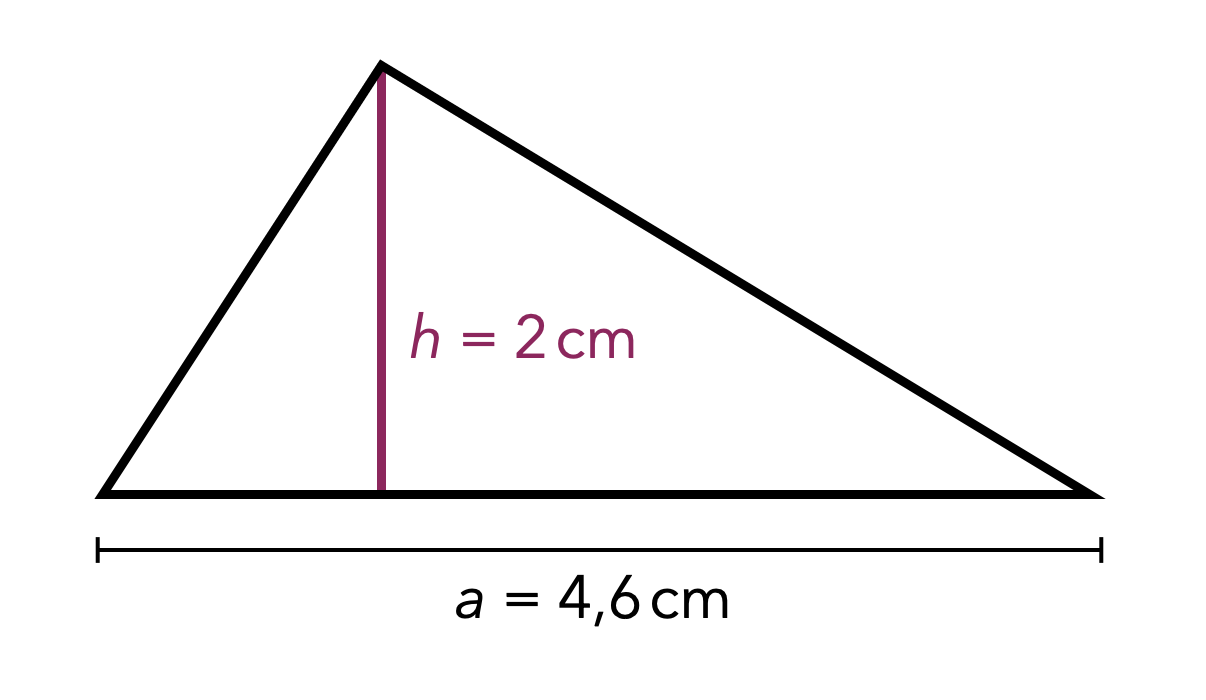
\includegraphics[width=0.5\linewidth]{pictures/8-Aufgabenorientierung} 

}

\caption{Flächeninhaltsbestimmung mit Musterorientierung}\label{fig:Aufgabenorientierung}
\end{figure}

Die Ermöglichung vielfältiger Orientierungsgrundlagen trägt damit auch zur Differenzierung des Unterrichts bei.

\hypertarget{aufgaben-gestalten-nachbereitung}{%
\section{Zum Nachbereiten}\label{aufgaben-gestalten-nachbereitung}}

Erstellen Sie zum Lerngegenstand \emph{Rechnen mit negativen Zahlen}

\begin{enumerate}
\def\labelenumi{\alph{enumi})}
\item
  jeweils eine Aufgabe zum Erkunden, Sichern, Üben und Vertiefen,
\item
  für die Vertiefungsaufgabe zwei bis drei gestufte Hilfen, sowie
\item
  eine Blütenaufgabe.
\end{enumerate}

\hypertarget{zweites-intermezzo}{%
\chapter{Zweites Intermezzo}\label{zweites-intermezzo}}

\hypertarget{part-inhaltsbezogene-kompetenzen}{%
\part*{Inhaltsbezogene Kompetenzen}\label{part-inhaltsbezogene-kompetenzen}}
\addcontentsline{toc}{part}{Inhaltsbezogene Kompetenzen}

\hypertarget{leitidee-zahl-und-operation}{%
\chapter{Leitidee Zahl und Operation}\label{leitidee-zahl-und-operation}}

\hypertarget{leitidee-messen-und-gruxf6uxdfen}{%
\chapter{Leitidee Messen und Größen}\label{leitidee-messen-und-gruxf6uxdfen}}

\hypertarget{leitidee-raum-und-form}{%
\chapter{Leitidee Raum und Form}\label{leitidee-raum-und-form}}

\hypertarget{leitidee-strukturen-und-funktionaler-zusammenhang}{%
\chapter{Leitidee Strukturen und funktionaler Zusammenhang}\label{leitidee-strukturen-und-funktionaler-zusammenhang}}

\hypertarget{leitidee-daten-und-zufall}{%
\chapter{Leitidee Daten und Zufall}\label{leitidee-daten-und-zufall}}

\hypertarget{appendix-anhang}{%
\appendix}


\hypertarget{seminar-und-hausarbeit}{%
\chapter{Seminar und Hausarbeit}\label{seminar-und-hausarbeit}}

\hypertarget{vollstuxe4ndiges-literaturverzeichnis}{%
\chapter{Vollständiges Literaturverzeichnis}\label{vollstuxe4ndiges-literaturverzeichnis}}

\hypertarget{refs}{}
\begin{CSLReferences}{1}{0}
\leavevmode\vadjust pre{\hypertarget{ref-Barzel2012a}{}}%
Barzel, B., Hußmann, S., Leuders, T., \& Prediger, S. (Hrsg.). (2012a). \emph{Mathewerkstatt. 5, {Handreichungen}} {[}DVD{]}. Cornelsen.

\leavevmode\vadjust pre{\hypertarget{ref-Barzel2012b}{}}%
Barzel, B., Hußmann, S., Leuders, T., \& Prediger, S. (Hrsg.). (2012b). \emph{Mathewerkstatt. 5, {Materialblock}} (Mittlerer Schulabschluss, allgemeine Ausg., 1. Aufl). Cornelsen.

\leavevmode\vadjust pre{\hypertarget{ref-Barzel2012}{}}%
Barzel, B., Hußmann, S., Leuders, T., \& Prediger, S. (Hrsg.). (2012c). \emph{Mathewerkstatt. 5, {Schulbuch}} (Mittlerer Schulabschluss, allgemeine Ausg., 1. Aufl.). Cornelsen.

\leavevmode\vadjust pre{\hypertarget{ref-Boeer2014}{}}%
Böer, H., Göckel, D., Kliemann, S., Koepsell, A., Puscher, R., Schmidt, W., \& Vernay, R. (2014). \emph{Mathe live. 8, {Schülerbuch}} (1. Aufl). Klett.

\leavevmode\vadjust pre{\hypertarget{ref-Bruckler:2018}{}}%
Brückler, F. M. (2018). \emph{Geschichte der {Mathematik} kompakt: {Das} {Wichtigste} aus {Analysis}, {Wahrscheinlichkeitstheorie}, angewandter {Mathematik}, {Topologie} und {Mengenlehre}}. Springer Spektrum. \url{https://doi.org/10.1007/978-3-662-55574-3}

\leavevmode\vadjust pre{\hypertarget{ref-Bruder}{}}%
Bruder, R. (o.~J.). \emph{Eine akzentuierte {Aufgabenauswahl} und {Vermitteln} heuristischer {Erfahrung} -- {Wege} zu einem anspruchsvollen {Mathematikunterricht} für alle}. Abgerufen 2. Januar 2022, von \url{http://www.math-learning.com/files/extremal.pdf}

\leavevmode\vadjust pre{\hypertarget{ref-Bruder1991}{}}%
Bruder, R. (1991). Unterrichtssituationen -- ein {Modell} für die {Aus}- und {Weiterbildung} zur {Gestaltung} von {Mathematikunterricht}. \emph{Wissenschaftliche Zeitschrift der Universität Potsdam}, \emph{35}(2), 129--134.

\leavevmode\vadjust pre{\hypertarget{ref-Bruder2011}{}}%
Bruder, R. (2001). Mathematik lernen und behalten. \emph{Pädagogik (Weinheim)}, \emph{53}(10), 15--18.

\leavevmode\vadjust pre{\hypertarget{ref-Bruder2012}{}}%
Bruder, R. (2012). Vielseitig mit {Aufgaben} arbeiten -- {Mathematische} {Kompetenzen} nachhaltig entwickeln und sichern. In R. Bruder, T. Leuders, \& A. Büchter (Hrsg.), \emph{Mathematikunterricht entwickeln} (S. 18--52). Cornelsen Scriptor.

\leavevmode\vadjust pre{\hypertarget{ref-Bruderb}{}}%
Bruder, R. (im {d}ruck). Orientierungsgrundlagen der {Lerntätigkeit} nach {Lompscher} -- {Potenziale} und {Einordnung} eines theoretischen {Konzepts}. In \emph{Beiträge zum {Mathematikunterricht} 2022}.

\leavevmode\vadjust pre{\hypertarget{ref-Bruder1989}{}}%
Bruder, R., \& Brückner, A. (1989). Zur {Beschreibung} von {Schülertätigkeiten} im {Mathematikunterricht} -- ein allgemeiner {Ansatz}. \emph{Pädagogische Forschung. Wissenschaftliche Nachrichten}, \emph{30}(6), 72--82.

\leavevmode\vadjust pre{\hypertarget{ref-Bruder2015a}{}}%
Bruder, R., Linneweber-Lammerskitten, H., \& Reibold, J. (2015). Individualisieren und differenzieren. In R. Bruder, L. Hefendehl-Hebeker, B. Schmidt-Thieme, \& H.-G. Weigand (Hrsg.), \emph{Handbuch der {Mathematikdidaktik}} (S. 513--534). Springer Berlin Heidelberg. \url{https://doi.org/10.1007/978-3-642-35119-8_19}

\leavevmode\vadjust pre{\hypertarget{ref-Bruner:1976}{}}%
Bruner, J. S. (1976). Die {Bedeutung} der {Struktur} im {Lernprozeß}. In A. Holtmann (Hrsg.), \emph{Das sozialwissenschaftliche {Curriculum} in der {Schule}: {Neue} {Formen} und {Inhalte}} (S. 77--90). VS Verlag für Sozialwissenschaften. \url{https://doi.org/10.1007/978-3-322-85275-5}

\leavevmode\vadjust pre{\hypertarget{ref-BundesministeriumfurErnahrungundLandwirtschaft2014}{}}%
Bundesministerium für Ernährung und Landwirtschaft. (2014). \emph{Gutachten über {Mindestanforderungen} an die {Haltung} von {Säugetieren}}. \url{https://www.bmel.de/SharedDocs/Downloads/DE/_Tiere/Tierschutz/HaltungSaeugetiere.pdf;jsessionid=6B0914AB410E7E118E6CC87C65735734.live832?__blob=publicationFile\&v=7}

\leavevmode\vadjust pre{\hypertarget{ref-Danckwerts:1988}{}}%
Danckwerts, R. (1988). Linearität als organisierendes Element zentraler Inhalte der Schulmathematik. \emph{Didaktik der Mathematik}, \emph{16}(2), 149--160.

\leavevmode\vadjust pre{\hypertarget{ref-Drijvers2010}{}}%
Drijvers, P., Doorman, M., Boon, P., Reed, H., \& Gravemeijer, K. (2010). The teacher and the tool: instrumental orchestrations in the technology-rich mathematics classroom. \emph{Educational Studies in Mathematics}, \emph{75}(2), 213--234. \url{https://doi.org/10.1007/s10649-010-9254-5}

\leavevmode\vadjust pre{\hypertarget{ref-Druke-Noe2018}{}}%
Drüke-Noe, C. (2018). Einfach -- mittel -- schwierig \ldots{} {Wenn} das so einfach wäre: {Aufgaben} unterschiedlichen {Schwierigkeitsgrades} entwickeln. \emph{mathematik lehren}, \emph{209}, 9--12.

\leavevmode\vadjust pre{\hypertarget{ref-Etzold:2019}{}}%
Etzold, H. (2019a). \emph{Winkel-{Farm}} (Version 2) {[}App{]}. \url{https://apps.apple.com/de/app/winkel-farm/id1369585218}

\leavevmode\vadjust pre{\hypertarget{ref-Etzold:2019Praxis4}{}}%
Etzold, H. (2019b). \emph{Winkel-{Farm} -- {Leitfaden} für {Lehrerinnen} und {Lehrer}} (Version 2). Zenodo. \url{https://doi.org/10.5281/zenodo.4747700}

\leavevmode\vadjust pre{\hypertarget{ref-Etzold2020a}{}}%
Etzold, H. (2020). \emph{Klipp {Klapp}} {[}App{]}. \url{https://apps.apple.com/de/app/klipp-klapp/id1157365733}

\leavevmode\vadjust pre{\hypertarget{ref-Etzold2021}{}}%
Etzold, H. (2021). \emph{Neue Zugänge zum Winkelbegriff} {[}Dissertation, Universität Potsdam{]}. \url{https://doi.org/10.25932/publishup-50418}

\leavevmode\vadjust pre{\hypertarget{ref-Etzold2018}{}}%
Etzold, H., Kortenkamp, U., \& Ladel, S. (2018). {ACAT}-{Review}-{Guide} -- {Ein} tätigkeitstheoretischer {Blick} auf die {Beurteilung} von {Mathematik}-{Apps}. In S. Ladel, U. Kortenkamp, \& H. Etzold (Hrsg.), \emph{Mathematik mit digitalen {Medien} -- konkret} (S. 91--98). WTM-Verlag. \url{https://doi.org/10.37626/GA9783959870788.0.07}

\leavevmode\vadjust pre{\hypertarget{ref-Feldt-Caesar2017}{}}%
Feldt-Caesar, N. (2017). \emph{Konzeptualisierung und {Diagnose} von mathematischem {Grundwissen} und {Grundkönnen}}. Springer Fachmedien Wiesbaden. \url{https://doi.org/10.1007/978-3-658-17373-9}

\leavevmode\vadjust pre{\hypertarget{ref-Fockler2018}{}}%
Föckler, F., Leuders, T., \& Holzäpfel, L. (2018). Die selbstdifferenzierende {Aufgabe} als {Form} der {Differenzierung} im {Mathematikunterricht}. In Fachgruppe Didaktik der Mathematik der Universität Paderborn (Hrsg.), \emph{Beiträge zum {Mathematikunterricht} 2018} (S. 541--544). WTM. \url{https://doi.org/10.17877/DE290R-19327}

\leavevmode\vadjust pre{\hypertarget{ref-Freudenthal:1973}{}}%
Freudenthal, H. (1973). \emph{Mathematik als pädagogische {Aufgabe}} (Bd. 2). Klett.

\leavevmode\vadjust pre{\hypertarget{ref-Giest2016a}{}}%
Giest, H. (2016). Kulturhistorische {Didaktik} und {Bildungstheorie}. \emph{Tätigkeitstheorie. Journal für tätigkeitstheoretische Forschung in Deutschland}, \emph{14}, 24--48. \url{http://www.ich-sciences.de/media/journal/Ausgabe_14/heft_14.pdf}

\leavevmode\vadjust pre{\hypertarget{ref-Giest2004a}{}}%
Giest, H., \& Lompscher, J. (2004). Tätigkeitstheoretische Überlegungen zu einer neuen {Lernkultur}. \emph{Sitzungsberichte der Leibniz-Sozietät}, \emph{72}, 101--123. \url{https://leibnizsozietaet.de/wp-content/uploads/2012/11/07_giest.pdf}

\leavevmode\vadjust pre{\hypertarget{ref-Giest2006}{}}%
Giest, H., \& Lompscher, J. (2006). \emph{Lerntätigkeit -- {Lernen} aus kultur-historischer {Perspektive}. {Ein} {Beitrag} zur {Entwicklung} einer neuen {Lernkultur} im {Unterricht}}. Lehmanns Media.

\leavevmode\vadjust pre{\hypertarget{ref-Greefrath2016}{}}%
Greefrath, G., Oldenburg, R., Siller, H.-S., Ulm, V., \& Weigand, H.-G. (2016). \emph{Didaktik der {Analysis}. {Aspekte} und {Grundvorstellungen} zentraler {Begriffe}} (F. Padberg \& A. Büchter, Hrsg.; 4. Aufl.). Springer Spektrum. \url{https://doi.org/10.1007/978-3-662-48877-5}

\leavevmode\vadjust pre{\hypertarget{ref-Hefendehl-Hebeker:2016}{}}%
Hefendehl-Hebeker, L. (2016). Subject-matter didactics in {German} traditions: {Early} historical developments. \emph{Journal für Mathematik-Didaktik}, \emph{37}(S1), 11--31. \url{https://doi.org/10.1007/s13138-016-0103-7}

\leavevmode\vadjust pre{\hypertarget{ref-Hussmann:2016}{}}%
Hußmann, S., \& Prediger, S. (2016). Specifying and Structuring Mathematical Topics: A Four-Level Approach for Combining Formal, Semantic, Concrete, and Empirical Levels Exemplified for Exponential Growth. \emph{Journal für Mathematik-Didaktik}, \emph{37}(S1), 33--67. \url{https://doi.org/10.1007/s13138-016-0102-8}

\leavevmode\vadjust pre{\hypertarget{ref-Hussmann:2016a}{}}%
Hußmann, S., Rezat, S., \& Sträßer, R. (2016). Subject {Matter} {Didactics} in {Mathematics} {Education}. \emph{Journal für Mathematik-Didaktik}, \emph{37}(S1), 1--9. \url{https://doi.org/10.1007/s13138-016-0105-5}

\leavevmode\vadjust pre{\hypertarget{ref-InstitutfurQualitatsentwicklungimBildungswesen2019}{}}%
Institut für Qualitätsentwicklung im Bildungswesen. (2019). \emph{Gemeinsame {Aufgabenpools} der {Länder}. {Aufgaben} für das {Fach} {Mathematik}. {Grundstock} von {Operatoren}}. \url{https://www.iqb.hu-berlin.de/abitur/abitur/dokumente/mathematik/M_Grundstock_von.pdf}

\leavevmode\vadjust pre{\hypertarget{ref-Jahnke:2010}{}}%
Jahnke, T. (2010). Vom mählichen {Verschwinden} des {Fachs} aus der {Mathematikdidaktik}. \emph{GDM-Mitteilungen 89}, 21--24. \url{https://ojs.didaktik-der-mathematik.de/index.php/mgdm/article/view/559/550}

\leavevmode\vadjust pre{\hypertarget{ref-Kleine2011a}{}}%
Kleine, M., \& Ludwig, M. (Hrsg.). (2011). \emph{Mathe.{Logo}. 7, {Gymnasium} {Thüringen}, {Schülerband}} (1. Auflage). C.C.Buchner.

\leavevmode\vadjust pre{\hypertarget{ref-Kortenkamp2018a}{}}%
Kortenkamp, U., Etzold, H., Goral, J., Schmidt, A., \& Börrnert, M. (2018). \emph{Digitale {Stellenwerttafel} -- {Leitfaden} für {Lehrerinnen} und {Lehrer} ({Version} 5)}. Zenodo. \url{https://doi.org/10.5281/zenodo.4761419}

\leavevmode\vadjust pre{\hypertarget{ref-Kortenkamp2019}{}}%
Kortenkamp, U., Etzold, H., \& Ladel, S. (2019). \emph{Leitfaden zur {Beurteilung} von {Apps}}. Zenodo. \url{https://doi.org/10.5281/zenodo.5091906}

\leavevmode\vadjust pre{\hypertarget{ref-Krainer:1989}{}}%
Krainer, K. (1989). \emph{Lebendige {Geometrie}. Überlegungen zu einem integrativen {Verständnis} von {Geometrieunterricht} anhand des {Winkelbegriffs}} {[}Dissertation{]}. Alpen-Adria-Universität Klagenfurt.

\leavevmode\vadjust pre{\hypertarget{ref-Krauthausen:2018}{}}%
Krauthausen, G. (2018). \emph{Einführung in die {Mathematikdidaktik}} (F. Padberg \& A. Büchter, Hrsg.; Mathematik Primarstufe und Sekundarstufe I + II). Springer Spektrum. \url{https://doi.org/10.1007/978-3-662-54692-5}

\leavevmode\vadjust pre{\hypertarget{ref-Krauthausen2010}{}}%
Krauthausen, G., \& Scherer, P. (2010). \emph{Umgang mit {Heterogenität}. {Natürliche} {Differenzierung} im {Mathematikunterricht} der {Grundschule}}. IPN. \url{http://www.sinus-an-grundschulen.de/fileadmin/uploads/Material_aus_SGS/Handreichung_Krauthausen-Scherer.pdf}

\leavevmode\vadjust pre{\hypertarget{ref-Kuntze2018}{}}%
Kuntze, S. (2018). Flächeninhalt und {Volumen}. In \emph{Didaktik der {Geometrie} für die {Sekundarstufe} {I}} (S. 149--177). Springer Berlin Heidelberg. \url{https://doi.org/10.1007/978-3-662-56217-8_7}

\leavevmode\vadjust pre{\hypertarget{ref-Kuzle}{}}%
Kuzle, A. (o.~J.). \emph{Theoretischer {Hintergrund} zum {Problemlösen}}. Abgerufen 9. Januar 2022, von \url{https://proffi-m.de/theorie}

\leavevmode\vadjust pre{\hypertarget{ref-Ladel2013}{}}%
Ladel, S., \& Kortenkamp, U. (2013). An {Activity}-{Theoretic} {Approach} to {Multi}-{Touch} {Tools} in {Early} {Mathematics} {Learning}. \emph{The International Journal for Technology in Mathematics Education}, \emph{1}(20), 3--8. \url{https://www.researchgate.net/publication/261823263_An_activity-theoretic_approach_to_multi-touch_tools_in_early_maths_learning}

\leavevmode\vadjust pre{\hypertarget{ref-Lambacher2010}{}}%
\emph{Lambacher {Schweizer} {Mathematik} für {Gymnasien}. 5, {Schülerbuch}} (Sachsen, 1. Aufl). (2010). {[}Computer software{]}. Klett.

\leavevmode\vadjust pre{\hypertarget{ref-Lambert:2012}{}}%
Lambert, A. (2012). \emph{Gedanken zum aktuellen {Kompetenzbegriff} für den ({Mathematik}-)unterricht} {[}Vortrag{]}. Eingangsstatement zur Podiumsdiskussion im Rahmen des 3. Fachdidaktischen Kolloquiums an der Universität des Saarlandes, Saarbrücken. \url{https://www.uni-saarland.de/fileadmin/upload/einrichtung/zfl/PDF_Fachdidaktik/PDF_Kolloquium_FD/Kompetenzbegriff_für_den_Mathematikunterricht_Statement_mit_Folien.pdf}

\leavevmode\vadjust pre{\hypertarget{ref-Larkin2019}{}}%
Larkin, K., Kortenkamp, U., Ladel, S., \& Etzold, H. (2019). Using the {ACAT} {Framework} to {Evaluate} the {Design} of {Two} {Geometry} {Apps}: an {Exploratory} {Study}. \emph{Digital Experiences in Mathematics Education}, \emph{5}(1), 59--92. \url{https://doi.org/10.1007/s40751-018-0045-4}

\leavevmode\vadjust pre{\hypertarget{ref-Leuders2009}{}}%
Leuders, T. (2009). Intelligent üben und {Mathematik} erleben. In T. Leuders, L. Hefendehl-Hebeker, \& H.-G. Weigand (Hrsg.), \emph{Mathemagische {Momente}} (S. 130--143). Cornelsen. \url{https://home.ph-freiburg.de/leudersfr/preprint/2009_leuders_intelligent_ueben_mathemagische_momente.pdf}

\leavevmode\vadjust pre{\hypertarget{ref-Leuders2015}{}}%
Leuders, T. (2015). Aufgaben in {Forschung} und {Praxis}. In R. Bruder, L. Hefendehl-Hebeker, B. Schmidt-Thieme, \& H.-G. Weigand (Hrsg.), \emph{Handbuch der {Mathematikdidaktik}} (S. 435--460). Springer Berlin Heidelberg. \url{https://doi.org/10.1007/978-3-642-35119-8}

\leavevmode\vadjust pre{\hypertarget{ref-Leuders2011}{}}%
Leuders, T., Hußmann, S., Barzel, B., \& Prediger, S. (2011). Das macht {Sinn}! {Sinnstiftung} mit {Kontexten} und {Kernideen}. \emph{Praxis der Mathematik in der Schule}, \emph{53}(37), 2--9. \url{https://www.researchgate.net/publication/233978329}

\leavevmode\vadjust pre{\hypertarget{ref-Barzel2015a}{}}%
Leuders, T., Prediger, S., Barzel, B., \& Hußmann, S. (Hrsg.). (2015). \emph{Mathewerkstatt. 7, {Schulbuch}} (Mittlerer Schulabschluss, allgemeine Ausg., 1. Aufl.). Cornelsen.

\leavevmode\vadjust pre{\hypertarget{ref-Lompscher1983a}{}}%
Lompscher, J. (1983a). Die {Ausbildung} von {Lernhandlungen}. In J. Lompscher (Hrsg.), \emph{Persönlichkeitsentwicklung in der {Lerntätigkeit}} (S. 53--78). Volk und Wissen.

\leavevmode\vadjust pre{\hypertarget{ref-Lompscher1983}{}}%
Lompscher, J. (1983b). Die {Lerntätigkeit} als dominierende {Tätigkeit} des jüngeren {Schülers}. In J. Lompscher (Hrsg.), \emph{Persönlichkeitsentwicklung in der {Lerntätigkeit}} (S. 23--52). Volk und Wissen.

\leavevmode\vadjust pre{\hypertarget{ref-Lompscher1996}{}}%
Lompscher, J. (1996). \emph{Aufsteigen vom {Abstrakten} zum {Konkreten} - {Lernen} und {Lehren} in {Zonen} der nächsten {Entwicklung}}. \url{https://publishup.uni-potsdam.de/opus4-ubp/frontdoor/deliver/index/docId/444/file/AUFSTEIG.pdf}

\leavevmode\vadjust pre{\hypertarget{ref-Mienert2011}{}}%
Mienert, M., \& Pitcher, S. (2011). \emph{Pädagogische {Psychologie}}. VS Verlag für Sozialwissenschaften. \url{https://doi.org/10.1007/978-3-531-92095-5}

\leavevmode\vadjust pre{\hypertarget{ref-MinisteriumfurBildungJugendundSportdesLandesBrandenburg}{}}%
Ministerium für Bildung, Jugend und Sport des Landes Brandenburg. (2015). \emph{Rahmenlehrplan {Brandenburg} {Sek}. {I}. {Teil} {B} - {Fachübergreifende} {Kompetenzentwicklung}}. \url{https://bildungsserver.berlin-brandenburg.de/fileadmin/bbb/unterricht/rahmenlehrplaene/Rahmenlehrplanprojekt/amtliche_Fassung/Teil_B_2015_11_10_WEB.pdf}

\leavevmode\vadjust pre{\hypertarget{ref-Mitchelmore:1990}{}}%
Mitchelmore, M. (1990). Psychologische und mathematische Schwierigkeiten beim Lernen des Winkelbegriffs. \emph{mathematica didactica}, \emph{13}, 19--37.

\leavevmode\vadjust pre{\hypertarget{ref-Mitchelmore:1998}{}}%
Mitchelmore, M., \& White, P. (1998). Development of {Angle} {Concepts}: {A} {Framework} for {Research}. \emph{Mathematics Education Research Journal}, \emph{10}(3), 4--27.

\leavevmode\vadjust pre{\hypertarget{ref-Padberg:2017}{}}%
Padberg, F., \& Wartha, S. (2017). \emph{Didaktik der {Bruchrechnung}} (5. Aufl.). Springer Spektrum. \url{https://doi.org/10.1007/978-3-662-52969-0}

\leavevmode\vadjust pre{\hypertarget{ref-Prediger2014}{}}%
Prediger, S., Hußmann, S., Leuders, T., \& Barzel, B. (2014). Kernprozesse -- {Ein} {Modell} zur {Strukturierung} von {Unterrichtsdesign} und {Unterrichtshandeln}. In I. Bausch, G. Pinkernell, \& O. Schmitt (Hrsg.), \emph{Unterrichtsentwicklung und {Kompetenzorientierung}. {Festschrift} für {Regina} {Bruder}} (S. 81--92). WTM. \url{https://www.researchgate.net/publication/261402528_Fachspezifische_Differenzierungsansatze_fur_unterschiedliche_Unterrichtsphasen}

\leavevmode\vadjust pre{\hypertarget{ref-Prediger2013}{}}%
Prediger, S., Leuders, T., Barzel, B., \& Hussmann, S. (2013). Anknüpfen, {Erkunden}, {Ordnen}, {Vertiefen}. In G. Greefrath, F. Käpnick, \& M. Stein (Hrsg.), \emph{Beiträge zum {Mathematikunterricht} 2013, 47. {Jahrestagung} der {Gesellschaft} für {Didaktik} der {Mathematik} vom 4.3.2013 bis 8.3.2013 in {Münster}} (S. 769--772). Gesellschaft für Didaktik der Mathematik. \url{https://doi.org/10.17877/DE290R-1474}

\leavevmode\vadjust pre{\hypertarget{ref-Quarder2020}{}}%
Quarder, J. (2020). \emph{Blütenaufgaben im {Mathematikunterricht}}. \url{https://www.youtube.com/watch?v=zrEimaARq7w}

\leavevmode\vadjust pre{\hypertarget{ref-Reitz-Koncebovski2018}{}}%
Reitz-Koncebovski, K., Kortenkamp, U., \& Goral, J. (2018). Gestaltungsprinzipien für fachwissenschaftliche {Einführungsveranstaltungen}. In A. Borowski, A. Ehlert, \& H. Prechtl (Hrsg.), \emph{{PSI}-{Potsdam}. {Ergebnisbericht} zu den {Aktivitäten} im {Rahmen} der {Qualitätsoffensive} {Lehrerbildung} (2015-2018)} (S. 175--188). Universitätsverlag Potsdam. \url{https://nbn-resolving.org/urn:nbn:de:kobv:517-opus4-420301}

\leavevmode\vadjust pre{\hypertarget{ref-Salle2021}{}}%
Salle, A., \& Clüver, T. (2021). Herleitung von {Grundvorstellungen} als normative {Leitlinien} -- {Beschreibung} eines theoriebasierten {Verfahrensrahmens}. \emph{Journal für Mathematik-Didaktik}. \url{https://doi.org/10.1007/s13138-021-00184-5}

\leavevmode\vadjust pre{\hypertarget{ref-Schecker2018}{}}%
Schecker, H., Wilhelm, T., Hopf, M., \& Duit, R. (Hrsg.). (2018). \emph{Schülervorstellungen und {Physikunterricht}: {Ein} {Lehrbuch} für {Studium}, {Referendariat} und {Unterrichtspraxis}}. Springer Berlin Heidelberg. \url{https://doi.org/10.1007/978-3-662-57270-2}

\leavevmode\vadjust pre{\hypertarget{ref-Schmidt-Thieme2015}{}}%
Schmidt-Thieme, B., \& Weigand, H.-G. (2015). Medien. In R. Bruder, L. Hefendehl-Hebeker, B. Schmidt-Thieme, \& H.-G. Weigand (Hrsg.), \emph{Handbuch der {Mathematikdidaktik}} (S. 461--490). Springer Berlin Heidelberg. \url{https://doi.org/10.1007/978-3-642-35119-8_17}

\leavevmode\vadjust pre{\hypertarget{ref-Schubert:2011}{}}%
Schubert, S., \& Schwill, A. (2011). \emph{Didaktik der {Informatik}} (2. Aufl). Spektrum, Akad. Verl. \url{https://doi.org/10.1007/978-3-8274-2653-6}

\leavevmode\vadjust pre{\hypertarget{ref-Schulz2018}{}}%
Schulz, A. (2018). Orientierung am {Zahlenstrahl} -- {Funktionen} und {Deutung}. In Fachgruppe Didaktik der Mathematik der Universität Paderborn (Hrsg.), \emph{Vorträge auf der 52. Tagung für Didaktik der Mathematik - Jahrestagung der Gesellschaft für Didaktik der Mathematik vom 05.03. bis 09.03.2018 in Paderborn} (S. 1663--1666). WTM-Verlag. \url{https://doi.org/10.17877/DE290R-19688}

\leavevmode\vadjust pre{\hypertarget{ref-Schupp:2016}{}}%
Schupp, H. (2016). Gedanken zum „{Stoff}`` und zur „{Stoffdidaktik}`` sowie zu ihrer {Bedeutung} für die {Qualität} des {Mathematikunterrichts}. \emph{Mathematische Semesterberichte}, \emph{63}(1), 69--92. \url{https://doi.org/10.1007/s00591-016-0159-y}

\leavevmode\vadjust pre{\hypertarget{ref-Schwill:1994}{}}%
Schwill, A. (1994). \emph{Fundamentale {Ideen} in {Mathematik} und {Informatik}}. Herbsttagung des Arbeitskreises Mathematikunterricht und Informatik, Wolfenbüttel. \url{http://www.informatikdidaktik.de/didaktik/Forschung/Wolfenbuettel94.pdf}

\leavevmode\vadjust pre{\hypertarget{ref-KMK:2012}{}}%
Sekretariat der Ständigen Konferenz der Kultusminister der Länder in der Bundesrepublik Deutschland. (2012). \emph{Bildungsstandards im {Fach} {Mathematik} für die {Allgemeine} {Hochschulreife}. (Beschluss der Kultusministerkonferenz vom 18.10.2012)}. \url{https://www.kmk.org/fileadmin/Dateien/veroeffentlichungen_beschluesse/2012/2012_10_18-Bildungsstandards-Mathe-Abi.pdf}

\leavevmode\vadjust pre{\hypertarget{ref-SekretariatderStandigenKonferenzderKultusministerderLanderinderBundesrepublikDeutschland2022}{}}%
Sekretariat der Ständigen Konferenz der Kultusminister der Länder in der Bundesrepublik Deutschland. (2022a). \emph{Bildungsstandards für das {Fach} {Mathematik} {Erster} {Schulabschluss} ({ESA}) und {Mittlerer} {Schulabschluss} ({MSA}). ({Beschluss} der {Kultusministerkonferenz} vom 15.10.2004 und vom 04.12.2003, i.d.{F}. vom 23.06.2022)}. \url{https://www.kmk.org/fileadmin/Dateien/veroeffentlichungen_beschluesse/2022/2022_06_23-Bista-ESA-MSA-Mathe.pdf}

\leavevmode\vadjust pre{\hypertarget{ref-SekretariatderStandigenKonferenzderKultusministerderLanderinderBundesrepublikDeutschland2022a}{}}%
Sekretariat der Ständigen Konferenz der Kultusminister der Länder in der Bundesrepublik Deutschland. (2022b). \emph{Bildungsstandards für das {Fach} {Mathematik} {Primarbereich}. ({Beschluss} der {Kultusministerkonferenz} vom 15.10.2004, i.d.{F}. vom 23.06.2022)}. \url{https://www.kmk.org/fileadmin/Dateien/veroeffentlichungen_beschluesse/2022/2022_06_23-Bista-Primarbereich-Mathe.pdf}

\leavevmode\vadjust pre{\hypertarget{ref-SINUSBayern}{}}%
SINUS Bayern. (o.~J.). \emph{Aufgabenkultur}. Abgerufen 2. Januar 2022, von \url{https://www.deltaplus.bayern.de/fileadmin/user_upload/DELTAplus/1_Aufgabenkultur/Aufgabenkultur.pdf}

\leavevmode\vadjust pre{\hypertarget{ref-Stein2018}{}}%
Stein, S. (2018). {ACAT}-{Review} zur {App} „{Klipp} {Klapp}``. In S. Ladel, U. Kortenkamp, \& H. Etzold (Hrsg.), \emph{Mathematik mit digitalen {Medien} -- konkret} (S. 121--128). WTM-Verlag. \url{https://doi.org/10.37626/GA9783959870788.0.10}

\leavevmode\vadjust pre{\hypertarget{ref-Steinhofel1988}{}}%
Steinhöfel, W., Reichold, K., \& Frenzel, L. (1988). \emph{Zur {Gestaltung} typischer {Unterrichtssituationen} im {Mathematikunterricht}}. Ministerium für Volksbildung.

\leavevmode\vadjust pre{\hypertarget{ref-Strehl:1983}{}}%
Strehl, R. (1983). Anschauliche {Vorstellung} und mathematische {Theorie} beim {Winkelbegriff}. \emph{mathematica didactica}, \emph{6}, 129--146.

\leavevmode\vadjust pre{\hypertarget{ref-Taylor:1715}{}}%
Taylor, B. (1715). \emph{Linear perspective}. printed for R. Knaplock at the Bishop's-Head in St. Paul's Church-Yard. \url{https://nl.sub.uni-goettingen.de/id/0590700700}

\leavevmode\vadjust pre{\hypertarget{ref-Thiel-Schneider2018}{}}%
Thiel-Schneider, A. (2018). \emph{Zum {Begriff} des exponentiellen {Wachstums}}. Springer Fachmedien Wiesbaden. \url{https://doi.org/10.1007/978-3-658-21895-9}

\leavevmode\vadjust pre{\hypertarget{ref-Tietze:2000a}{}}%
Tietze, U.-P., Klika, M., \& Wolpers, H. (Hrsg.). (2000a). \emph{Mathematikunterricht in der {Sekundarstufe} {II}. {Band} 1: {Fachdidaktische} {Grundfragen}, {Didaktik} der {Analysis}} (2. Aufl.). Vieweg+Teubner Verlag. \url{https://doi.org/10.1007/978-3-322-90568-0}

\leavevmode\vadjust pre{\hypertarget{ref-Tietze:2000}{}}%
Tietze, U.-P., Klika, M., \& Wolpers, H. (Hrsg.). (2000b). \emph{Mathematikunterricht in der {Sekundarstufe} {II}. {Band} 2: {Didaktik} der {Analytischen} {Geometrie} und {Linearen} {Algebra}}. Vieweg+Teubner Verlag. \url{https://doi.org/10.1007/978-3-322-86479-6}

\leavevmode\vadjust pre{\hypertarget{ref-Tietze:2002}{}}%
Tietze, U.-P., Klika, M., \& Wolpers, H. (Hrsg.). (2002). \emph{Mathematikunterricht in der {Sekundarstufe} {II}. {Band} 3: {Didaktik} der {Stochastik}}. Vieweg+Teubner Verlag. \url{https://doi.org/10.1007/978-3-322-83144-6}

\leavevmode\vadjust pre{\hypertarget{ref-vandenHeuvel-Panhuizen2003}{}}%
van den Heuvel-Panhuizen, M. (2003). The didactical use of models in realistic mathematics education: {An} example from a longitudinal trajectory on percentage. \emph{Educational Studies in Mathematics}, \emph{54}, 9--35. \url{https://doi.org/10.1023/B:EDUC.0000005212.03219.dc}

\leavevmode\vadjust pre{\hypertarget{ref-Vohns:2000}{}}%
Vohns, A. (2000). \emph{Das {Messen} als fundamentale {Idee}} {[}1. Staatsexamensarbeit, Universität-Gesamthochschule Siegen{]}. \url{https://wwwu.aau.at/avohns/pdf/messen.pdf}

\leavevmode\vadjust pre{\hypertarget{ref-Hofe:1995}{}}%
vom Hofe, R. (1995). \emph{Grundvorstellungen mathematischer {Inhalte}}. Spektrum Akademischer Verlag.

\leavevmode\vadjust pre{\hypertarget{ref-vomHofe2014}{}}%
vom Hofe, R. (2014). Primäre und sekundäre {Grundvorstellungen}. In J. Roth \& J. Ames (Hrsg.), \emph{Beiträge zum {Mathematikunterricht} 2014, 48. {Jahrestagung} der {Gesellschaft} für {Didaktik} der {Mathematik} vom 10.03.2014 bis 14.03.2014 in {Koblenz}}. WTM. \url{https://doi.org/10.17877/DE290R-8808}

\leavevmode\vadjust pre{\hypertarget{ref-vonderBank:2013}{}}%
von der Bank, M.-C. (2013). Fundamentale {Ideen}, insbesondere {Optimierung}. In A. Filler \& M. Ludwig (Hrsg.), \emph{Wege zur {Begriffsbildung} für den {Geometrieunterricht}. {Ziele} und {Visionen} 2020. {Vorträge} auf der 29. {Herbsttagung} des {Arbeitskreises} {Geometrie} in der {Gesellschaft} für {Didaktik} der {Mathematik} vom 14. bis 16. {September} 2012 in {Saarbrücken}} (S. 83--124). Franzbecker. \url{https://www.math.uni-sb.de/service/lehramt/AKGeometrie/AKGeometrie2012.pdf}

\leavevmode\vadjust pre{\hypertarget{ref-Bank:2016}{}}%
von der Bank, M.-C. (2016). \emph{Fundamentale {Ideen} der {Mathematik}: {Weiterentwicklung} einer {Theorie} zu deren unterrichtspraktischer {Nutzung}} {[}Dissertation, Universität des Saarlandes{]}. \url{https://doi.org/10.22028/D291-26673}

\leavevmode\vadjust pre{\hypertarget{ref-Wartha2011}{}}%
Wartha, S., \& Schulz, A. (2011). \emph{Aufbau von {Grundvorstellungen} (nicht nur) bei besonderen {Schwierigkeiten} im {Rechnen}}. IPN Kiel. \url{http://www.sinus-an-grundschulen.de/fileadmin/uploads/Material_aus_SGS/Handreichung_WarthaSchulz.pdf}

\leavevmode\vadjust pre{\hypertarget{ref-WikiPeano}{}}%
Wikipedia. (2021). \emph{Peano-Axiome --- Wikipedia{,} die freie Enzyklopädie}. \url{https://de.wikipedia.org/w/index.php?title=Peano-Axiome\&oldid=216675163}

\leavevmode\vadjust pre{\hypertarget{ref-WikiKerze}{}}%
Wikipedia. (2022). \emph{Kerzenuhr --- Wikipedia{,} die freie Enzyklopädie}. \url{https://de.wikipedia.org/w/index.php?title=Kerzenuhr\&oldid=227115991}

\leavevmode\vadjust pre{\hypertarget{ref-enwiki:1023437370}{}}%
Wikipedia contributors. (2021). \emph{Manipulative (mathematics education) --- {Wikipedia}{,} The Free Encyclopedia}. \url{https://en.wikipedia.org/w/index.php?title=Manipulative_(mathematics_education)\&oldid=1023437370}

\leavevmode\vadjust pre{\hypertarget{ref-Wittmann:2015}{}}%
Wittmann, E. C. (2015). Strukturgenetische didaktische {Analysen} -- empirische {Forschung} „erster {Art}``. \emph{mathematica didactica}, 239--255. \url{http://www.mathematica-didactica.com/altejahrgaenge/md_2015/md_2015_Wittmann_Stoffdidaktik.pdf}

\leavevmode\vadjust pre{\hypertarget{ref-Worner2014}{}}%
Wörner, D. (2014). Grundvorstellungen zum {Flächeninhaltsbegriff} ausbilden -- eine exemplarische {Studie}. In J. Roth \& J. Ames (Hrsg.), \emph{Beiträge zum {Mathematikunterricht} 2014, 48. {Jahrestagung} der {Gesellschaft} für {Didaktik} der {Mathematik} vom 10.03.2014 bis 14.03.2014 in {Koblenz}} (S. 1327--1330). \url{https://doi.org/10.17877/DE290R-1049}

\leavevmode\vadjust pre{\hypertarget{ref-Wygotski1985a}{}}%
Wygotski, L. (1985). Die instrumentelle {Methode} in der {Psychologie}. In J. Lompscher (Hrsg.), \emph{Lew {Wygotski}. {Ausgewählte} {Schriften}. {Teil} 1: {Arbeiten} zu theoretischen und methodologischen {Problemen} der {Psychologie}} (S. 309--317). Volk und Wissen.

\leavevmode\vadjust pre{\hypertarget{ref-Zech1998}{}}%
Zech, F. (1998). \emph{Grundkurs {Mathematikdidaktik}} (9. Aufl.). Beltz Verlag.

\end{CSLReferences}

\printindex

\end{document}
